\documentclass[a4paper]{book}
\usepackage{a4wide}
\usepackage{makeidx}
\usepackage{fancyhdr}
\usepackage{graphicx}
\usepackage{multicol}
\usepackage{float}
\usepackage{listings}
\usepackage{color}
\usepackage{textcomp}
\usepackage{alltt}
\usepackage{times}
\usepackage{ifpdf}
\ifpdf
\usepackage[pdftex,
            pagebackref=true,
            colorlinks=true,
            linkcolor=blue,
            unicode
           ]{hyperref}
\else
\usepackage[ps2pdf,
            pagebackref=true,
            colorlinks=true,
            linkcolor=blue,
            unicode
           ]{hyperref}
\usepackage{pspicture}
\fi
\usepackage[utf8]{inputenc}
\usepackage{doxygen}
\lstset{language=C++,inputencoding=utf8,basicstyle=\footnotesize,breaklines=true,breakatwhitespace=true,tabsize=8,numbers=left }
\makeindex
\setcounter{tocdepth}{3}
\renewcommand{\footrulewidth}{0.4pt}
\begin{document}
\hypersetup{pageanchor=false}
\begin{titlepage}
\vspace*{7cm}
\begin{center}
{\Large Reference Manual}\\
\vspace*{1cm}
{\large Generated by Doxygen 1.5.9}\\
\vspace*{0.5cm}
{\small Tue Jun 8 13:06:15 2010}\\
\end{center}
\end{titlepage}
\clearemptydoublepage
\pagenumbering{roman}
\tableofcontents
\clearemptydoublepage
\pagenumbering{arabic}
\hypersetup{pageanchor=true}
\chapter{Smoothed-particle hydrodynamics (SPH) code}
\label{index}\hypertarget{index}{}\hypertarget{index_intro_sec}{}\section{Introduction}\label{index_intro_sec}
SPH and SDPD 2D code\hypertarget{index_install_sec}{}\section{Installation}\label{index_install_sec}
Check the source code from github and compile 

\begin{footnotesize}\begin{verbatim}
   git clone git://github.com/slitvinov/sph-blitz
   cd sph-blitz
   ./local-install.sh  \end{verbatim}
\end{footnotesize}
\hypertarget{index_restart_file}{}\section{Restart file format}\label{index_restart_file}
\hypertarget{index_input_file}{}\section{Input file format}\label{index_input_file}
\hypertarget{index_sim}{}\section{Runnig simulations}\label{index_sim}


\begin{footnotesize}\begin{verbatim}
   cd src
   ./sph ../cases/couette \end{verbatim}
\end{footnotesize}
 \hypertarget{index_post}{}\section{Postprocessing}\label{index_post}
To combine all time snapshots in one file 

\begin{footnotesize}\begin{verbatim}
   cd outdata/
   ../../scripts/dat2punto.sh > punto.dat
 \end{verbatim}
\end{footnotesize}
\hypertarget{index_vis}{}\section{Visuzalization}\label{index_vis}
\hypertarget{index_vis_gnuplot}{}\subsection{gnuplot}\label{index_vis_gnuplot}
 \hypertarget{index_vis_punto}{}\subsection{punto}\label{index_vis_punto}


\begin{footnotesize}\begin{verbatim}
    punto -D 2 -c 4 -B 0:0:0.04:0.04 -G -0.6:0.6 -s 8 -lc black -bg white  punto.dat \end{verbatim}
\end{footnotesize}
  
\chapter{Class Index}
\section{Class Hierarchy}
This inheritance list is sorted roughly, but not completely, alphabetically:\begin{CompactList}
\item \contentsline{section}{Boundary}{\pageref{classBoundary}}{}
\item \contentsline{section}{Diagnose}{\pageref{classDiagnose}}{}
\item \contentsline{section}{Force}{\pageref{classForce}}{}
\item \contentsline{section}{Hydrodynamics}{\pageref{classHydrodynamics}}{}
\item \contentsline{section}{Initiation}{\pageref{classInitiation}}{}
\item \contentsline{section}{Interaction}{\pageref{classInteraction}}{}
\item \contentsline{section}{Kernel}{\pageref{classKernel}}{}
\begin{CompactList}
\item \contentsline{section}{BetaSpline}{\pageref{classBetaSpline}}{}
\item \contentsline{section}{QuinticSpline}{\pageref{classQuinticSpline}}{}
\end{CompactList}
\item \contentsline{section}{Llist$<$ Ldata $>$}{\pageref{classLlist}}{}
\item \contentsline{section}{LlistNode$<$ Ldata $>$}{\pageref{classLlistNode}}{}
\item \contentsline{section}{Material}{\pageref{classMaterial}}{}
\item \contentsline{section}{MLS}{\pageref{classMLS}}{}
\item \contentsline{section}{Output}{\pageref{classOutput}}{}
\item \contentsline{section}{Particle}{\pageref{classParticle}}{}
\item \contentsline{section}{ParticleManager}{\pageref{classParticleManager}}{}
\item \contentsline{section}{TimeSolver}{\pageref{classTimeSolver}}{}
\item \contentsline{section}{Wiener}{\pageref{classWiener}}{}
\end{CompactList}

\chapter{Class Index}
\section{Class List}
Here are the classes, structs, unions and interfaces with brief descriptions:\begin{CompactList}
\item\contentsline{section}{\hyperlink{classBetaSpline}{BetaSpline} (A concrete kernel class )}{\pageref{classBetaSpline}}{}
\item\contentsline{section}{\hyperlink{classBoundary}{Boundary} (\hyperlink{classBoundary}{Boundary} conditions )}{\pageref{classBoundary}}{}
\item\contentsline{section}{\hyperlink{classDiagnose}{Diagnose} (\hyperlink{classOutput}{Output} diagnosal )}{\pageref{classDiagnose}}{}
\item\contentsline{section}{\hyperlink{classForce}{Force} (The class defining force on or between particles )}{\pageref{classForce}}{}
\item\contentsline{section}{\hyperlink{classHydrodynamics}{Hydrodynamics} (Definition of materials and their hydrodynamical interactions )}{\pageref{classHydrodynamics}}{}
\item\contentsline{section}{\hyperlink{classInitiation}{Initiation} (Initiates the simulation )}{\pageref{classInitiation}}{}
\item\contentsline{section}{\hyperlink{classInteraction}{Interaction} (Defines interaction between particles )}{\pageref{classInteraction}}{}
\item\contentsline{section}{\hyperlink{classKernel}{Kernel} (\hyperlink{classKernel}{Kernel} abstract base )}{\pageref{classKernel}}{}
\item\contentsline{section}{\hyperlink{classLlist}{Llist$<$ Ldata $>$} (Double linked list implementation )}{\pageref{classLlist}}{}
\item\contentsline{section}{\hyperlink{classLlistNode}{LlistNode$<$ Ldata $>$} (A template node in the linked list )}{\pageref{classLlistNode}}{}
\item\contentsline{section}{\hyperlink{classMaterial}{Material} (\hyperlink{classMaterial}{Material} )}{\pageref{classMaterial}}{}
\item\contentsline{section}{\hyperlink{classMLS}{MLS} (Moving Least Squares (\hyperlink{classMLS}{MLS}) class )}{\pageref{classMLS}}{}
\item\contentsline{section}{\hyperlink{classOutput}{Output} (\hyperlink{classOutput}{Output} class )}{\pageref{classOutput}}{}
\item\contentsline{section}{\hyperlink{classParticle}{Particle} (\hyperlink{classParticle}{Particle} class )}{\pageref{classParticle}}{}
\item\contentsline{section}{\hyperlink{classParticleManager}{ParticleManager} (\hyperlink{classParticle}{Particle} manager class )}{\pageref{classParticleManager}}{}
\item\contentsline{section}{\hyperlink{classQuinticSpline}{QuinticSpline} (Quintic spline class )}{\pageref{classQuinticSpline}}{}
\item\contentsline{section}{\hyperlink{classTimeSolver}{TimeSolver} (Time solver class )}{\pageref{classTimeSolver}}{}
\item\contentsline{section}{\hyperlink{classWiener}{Wiener} (\hyperlink{classWiener}{Wiener} process )}{\pageref{classWiener}}{}
\end{CompactList}

\chapter{File Index}
\section{File List}
Here is a list of all documented files with brief descriptions:\begin{CompactList}
\item\contentsline{section}{\hyperlink{betaspline_8h}{betaspline.h} (Beta spline kernel function )}{\pageref{betaspline_8h}}{}
\item\contentsline{section}{\hyperlink{boundary_8cpp}{boundary.cpp} }{\pageref{boundary_8cpp}}{}
\item\contentsline{section}{\hyperlink{boundary_8h}{boundary.h} (Bonudary conditions )}{\pageref{boundary_8h}}{}
\item\contentsline{section}{\hyperlink{bskernel_8cpp}{bskernel.cpp} }{\pageref{bskernel_8cpp}}{}
\item\contentsline{section}{\hyperlink{diagnose_8h}{diagnose.h} (\hyperlink{classOutput}{Output} the diagnosal results )}{\pageref{diagnose_8h}}{}
\item\contentsline{section}{\hyperlink{diagose_8cpp}{diagose.cpp} }{\pageref{diagose_8cpp}}{}
\item\contentsline{section}{\hyperlink{dllist_8h}{dllist.h} (Double linked list implementation )}{\pageref{dllist_8h}}{}
\item\contentsline{section}{\hyperlink{force_8h}{force.h} (The class defining force on or between particles )}{\pageref{force_8h}}{}
\item\contentsline{section}{\hyperlink{glbcls_8h}{glbcls.h} (Global class declarations )}{\pageref{glbcls_8h}}{}
\item\contentsline{section}{\hyperlink{glbfunc_8cpp}{glbfunc.cpp} }{\pageref{glbfunc_8cpp}}{}
\item\contentsline{section}{\hyperlink{glbfunc_8h}{glbfunc.h} }{\pageref{glbfunc_8h}}{}
\item\contentsline{section}{\hyperlink{hydrodynamics_8cpp}{hydrodynamics.cpp} }{\pageref{hydrodynamics_8cpp}}{}
\item\contentsline{section}{\hyperlink{hydrodynamics_8h}{hydrodynamics.h} (Definition of materials and their hydrodynamical interactions )}{\pageref{hydrodynamics_8h}}{}
\item\contentsline{section}{\hyperlink{initiation_8cpp}{initiation.cpp} }{\pageref{initiation_8cpp}}{}
\item\contentsline{section}{\hyperlink{initiation_8h}{initiation.h} (Initiates the simulation )}{\pageref{initiation_8h}}{}
\item\contentsline{section}{\hyperlink{interaction_8cpp}{interaction.cpp} }{\pageref{interaction_8cpp}}{}
\item\contentsline{section}{\hyperlink{interaction_8h}{interaction.h} (Defines interaction between particles )}{\pageref{interaction_8h}}{}
\item\contentsline{section}{\hyperlink{kernel_8cpp}{kernel.cpp} (Abstract kernel base class )}{\pageref{kernel_8cpp}}{}
\item\contentsline{section}{\hyperlink{kernel_8h}{kernel.h} (\hyperlink{classKernel}{Kernel} abstract base )}{\pageref{kernel_8h}}{}
\item\contentsline{section}{\hyperlink{material_8cpp}{material.cpp} }{\pageref{material_8cpp}}{}
\item\contentsline{section}{\hyperlink{material_8h}{material.h} (\hyperlink{classMaterial}{Material} )}{\pageref{material_8h}}{}
\item\contentsline{section}{\hyperlink{mls_8cpp}{mls.cpp} }{\pageref{mls_8cpp}}{}
\item\contentsline{section}{\hyperlink{mls_8h}{mls.h} }{\pageref{mls_8h}}{}
\item\contentsline{section}{\hyperlink{output_8cpp}{output.cpp} }{\pageref{output_8cpp}}{}
\item\contentsline{section}{\hyperlink{output_8h}{output.h} (\hyperlink{classOutput}{Output} the computational results )}{\pageref{output_8h}}{}
\item\contentsline{section}{\hyperlink{particle_8cpp}{particle.cpp} }{\pageref{particle_8cpp}}{}
\item\contentsline{section}{\textbf{particle.h} }{\pageref{particle_8h}}{}
\item\contentsline{section}{\hyperlink{particlemanager_8h}{particlemanager.h} (\hyperlink{classParticle}{Particle} manager )}{\pageref{particlemanager_8h}}{}
\item\contentsline{section}{\hyperlink{quinticspline_8cpp}{quinticspline.cpp} }{\pageref{quinticspline_8cpp}}{}
\item\contentsline{section}{\hyperlink{quinticspline_8h}{quinticspline.h} (Quintic spline kernel )}{\pageref{quinticspline_8h}}{}
\item\contentsline{section}{\hyperlink{sph_8cpp}{sph.cpp} }{\pageref{sph_8cpp}}{}
\item\contentsline{section}{\hyperlink{timesolver_8cpp}{timesolver.cpp} }{\pageref{timesolver_8cpp}}{}
\item\contentsline{section}{\hyperlink{timesolver_8h}{timesolver.h} (Time solver class )}{\pageref{timesolver_8h}}{}
\item\contentsline{section}{\hyperlink{vec2d_8h}{vec2d.h} (Define 2-d vectors and associated operations )}{\pageref{vec2d_8h}}{}
\item\contentsline{section}{\hyperlink{wiener_8h}{wiener.h} (\hyperlink{classWiener}{Wiener} process )}{\pageref{wiener_8h}}{}
\end{CompactList}

\chapter{Class Documentation}
\hypertarget{classBetaSpline}{
\section{BetaSpline Class Reference}
\label{classBetaSpline}\index{BetaSpline@{BetaSpline}}
}
A concrete kernel class.  


{\tt \#include $<$betaspline.h$>$}

Inheritance diagram for BetaSpline:\nopagebreak
\begin{figure}[H]
\begin{center}
\leavevmode
\includegraphics[width=106pt]{classBetaSpline__inherit__graph}
\end{center}
\end{figure}
Collaboration diagram for BetaSpline:\nopagebreak
\begin{figure}[H]
\begin{center}
\leavevmode
\includegraphics[width=106pt]{classBetaSpline__coll__graph}
\end{center}
\end{figure}
\subsection*{Public Member Functions}
\begin{CompactItemize}
\item 
\hyperlink{classBetaSpline_00e744e584e6e7291813ab5e59d801ec}{BetaSpline} (double \hyperlink{classKernel_f088821dba4a00d1d320b27ebcb71258}{smoothingLength})
\begin{CompactList}\small\item\em constructor to initialize the data members and \item\end{CompactList}\item 
virtual double \hyperlink{classBetaSpline_797016b36239b0be98c3aa0715bb045a}{w} (double distance) const 
\begin{CompactList}\small\item\em Calculates the kernel value for the given distance of two particles. \item\end{CompactList}\item 
virtual Vec2d \hyperlink{classBetaSpline_409d22f7b4165a612ffbb62400e55db7}{gradW} (double distance, const Vec2d \&distanceVector) const 
\begin{CompactList}\small\item\em Calculates the kernel derivation for the given distance of two particles. \item\end{CompactList}\item 
\hypertarget{classBetaSpline_5b01a3303b3d45e74cdbff21419a07ff}{
double \hyperlink{classBetaSpline_5b01a3303b3d45e74cdbff21419a07ff}{F} (double distance) const }
\label{classBetaSpline_5b01a3303b3d45e74cdbff21419a07ff}

\begin{CompactList}\small\item\em Calculates the kernel derivation to distance. \item\end{CompactList}\end{CompactItemize}
\subsection*{Private Attributes}
\begin{CompactItemize}
\item 
\hypertarget{classBetaSpline_3cc93fb702c723e280f4c55aa7422def}{
double \hyperlink{classBetaSpline_3cc93fb702c723e280f4c55aa7422def}{norm}}
\label{classBetaSpline_3cc93fb702c723e280f4c55aa7422def}

\begin{CompactList}\small\item\em Normalization factor. \item\end{CompactList}\item 
\hypertarget{classBetaSpline_ca1e84910928d93dc2b7f4586f1102ac}{
double \hyperlink{classBetaSpline_ca1e84910928d93dc2b7f4586f1102ac}{reciprocH}}
\label{classBetaSpline_ca1e84910928d93dc2b7f4586f1102ac}

\begin{CompactList}\small\item\em Auxiliary factors for intermediate results: The inverse smoothing length $\ast$/. \item\end{CompactList}\item 
\hypertarget{classBetaSpline_06df50a142cacc03bfd3168cc6ae1f57}{
double \hyperlink{classBetaSpline_06df50a142cacc03bfd3168cc6ae1f57}{factorW}}
\label{classBetaSpline_06df50a142cacc03bfd3168cc6ae1f57}

\begin{CompactList}\small\item\em Auxiliary factors for intermediate results: A pre-factor for w $\ast$/. \item\end{CompactList}\item 
\hypertarget{classBetaSpline_0b285867c4f1d4b9fced5847650a47f8}{
double \hyperlink{classBetaSpline_0b285867c4f1d4b9fced5847650a47f8}{factorGradW}}
\label{classBetaSpline_0b285867c4f1d4b9fced5847650a47f8}

\begin{CompactList}\small\item\em Auxiliary factors for intermediate results: A pre-factor for grad w $\ast$/. \item\end{CompactList}\end{CompactItemize}


\subsection{Detailed Description}
A concrete kernel class. 

see Monaghan \& Lattanzio (1985) most often used kernel implemented in \hyperlink{bskernel_8cpp}{bskernel.cpp} 

\subsection{Constructor \& Destructor Documentation}
\hypertarget{classBetaSpline_00e744e584e6e7291813ab5e59d801ec}{
\index{BetaSpline@{BetaSpline}!BetaSpline@{BetaSpline}}
\index{BetaSpline@{BetaSpline}!BetaSpline@{BetaSpline}}
\subsubsection[{BetaSpline}]{\setlength{\rightskip}{0pt plus 5cm}BetaSpline::BetaSpline (double {\em smoothingLength})}}
\label{classBetaSpline_00e744e584e6e7291813ab5e59d801ec}


constructor to initialize the data members and 



\begin{itemize}
\item initialize the auxiliary factors\end{itemize}


\begin{itemize}
\item normalize to 1.0 \end{itemize}


\subsection{Member Function Documentation}
\hypertarget{classBetaSpline_409d22f7b4165a612ffbb62400e55db7}{
\index{BetaSpline@{BetaSpline}!gradW@{gradW}}
\index{gradW@{gradW}!BetaSpline@{BetaSpline}}
\subsubsection[{gradW}]{\setlength{\rightskip}{0pt plus 5cm}Vec2d BetaSpline::gradW (double {\em distance}, \/  const Vec2d \& {\em distanceVector}) const\hspace{0.3cm}{\tt  \mbox{[}virtual\mbox{]}}}}
\label{classBetaSpline_409d22f7b4165a612ffbb62400e55db7}


Calculates the kernel derivation for the given distance of two particles. 

We take this from Monaghan \& Lattenzio (1985) but used a doubled smoothing length for the definition of the interaction radius. 

Implements \hyperlink{classKernel_545e61b98db05db6dd02b88e2ad3da23}{Kernel}.\hypertarget{classBetaSpline_797016b36239b0be98c3aa0715bb045a}{
\index{BetaSpline@{BetaSpline}!w@{w}}
\index{w@{w}!BetaSpline@{BetaSpline}}
\subsubsection[{w}]{\setlength{\rightskip}{0pt plus 5cm}double BetaSpline::w (double {\em distance}) const\hspace{0.3cm}{\tt  \mbox{[}virtual\mbox{]}}}}
\label{classBetaSpline_797016b36239b0be98c3aa0715bb045a}


Calculates the kernel value for the given distance of two particles. 

We take this from Monaghan \& Lattenzio (1985) but used a doubled smoothing length for the definition of the interaction radius. 

Implements \hyperlink{classKernel_6b4d26ba99457a4acbbbca1454dbdc8a}{Kernel}.

The documentation for this class was generated from the following files:\begin{CompactItemize}
\item 
\hyperlink{betaspline_8h}{betaspline.h}\item 
\hyperlink{bskernel_8cpp}{bskernel.cpp}\end{CompactItemize}

\hypertarget{classBoundary}{
\section{Boundary Class Reference}
\label{classBoundary}\index{Boundary@{Boundary}}
}
\hyperlink{classBoundary}{Boundary} conditions.  


{\tt \#include $<$boundary.h$>$}

Collaboration diagram for Boundary:\nopagebreak
\begin{figure}[H]
\begin{center}
\leavevmode
\includegraphics[width=192pt]{classBoundary__coll__graph}
\end{center}
\end{figure}
\subsection*{Public Member Functions}
\begin{CompactItemize}
\item 
\hyperlink{classBoundary_8fe88473063d74e67a5932f2e4d2e517}{Boundary} (\hyperlink{classInitiation}{Initiation} \&ini, \hyperlink{classHydrodynamics}{Hydrodynamics} \&hydro, \hyperlink{classParticleManager}{ParticleManager} \&particles)
\begin{CompactList}\small\item\em boundary particle list for all boundray particles \item\end{CompactList}\item 
void \hyperlink{classBoundary_8a40f99b73f3622cd5f1387fcbbdb824}{BuildBoundaryParticles} (\hyperlink{classParticleManager}{ParticleManager} \&particles, \hyperlink{classHydrodynamics}{Hydrodynamics} \&hydro)
\begin{CompactList}\small\item\em build boundary particles \item\end{CompactList}\item 
void \hyperlink{classBoundary_bedd190ee91482e4e59b2a613ab25d57}{BoundaryCondition} (\hyperlink{classParticleManager}{ParticleManager} \&particles)
\begin{CompactList}\small\item\em boundary conditions \item\end{CompactList}\item 
void \hyperlink{classBoundary_ac37e18aaf60503a66173d9428ed9e54}{RunAwayCheck} (\hyperlink{classHydrodynamics}{Hydrodynamics} \&hydro)
\begin{CompactList}\small\item\em check particle if particle run out of the computational domain \item\end{CompactList}\end{CompactItemize}
\subsection*{Public Attributes}
\begin{CompactItemize}
\item 
int \hyperlink{classBoundary_10dd58ba0715412968c4902fe80b1318}{xBl}
\begin{CompactList}\small\item\em boundary condition indicator left hand side \item\end{CompactList}\item 
int \hyperlink{classBoundary_4a582b489cb580b8a6f3a7123f411a53}{xBr}
\begin{CompactList}\small\item\em boundary condition indicator right hand side \item\end{CompactList}\item 
int \hyperlink{classBoundary_0329bf6b954b3001418391cc16a9194e}{yBd}
\begin{CompactList}\small\item\em boundary condition indicator bottom side \item\end{CompactList}\item 
int \hyperlink{classBoundary_6ccff2a8c5a10104d202504034af9e84}{yBu}
\begin{CompactList}\small\item\em boundary condition indicator upper side \item\end{CompactList}\item 
\hypertarget{classBoundary_238a4e6e7358e1f9a2375d8df08a5c7a}{
Vec2d \hyperlink{classBoundary_238a4e6e7358e1f9a2375d8df08a5c7a}{UxBl}}
\label{classBoundary_238a4e6e7358e1f9a2375d8df08a5c7a}

\begin{CompactList}\small\item\em left hand side boundary velocity \item\end{CompactList}\item 
\hypertarget{classBoundary_375a949ddac9f633af007daa7d323099}{
Vec2d \hyperlink{classBoundary_375a949ddac9f633af007daa7d323099}{UxBr}}
\label{classBoundary_375a949ddac9f633af007daa7d323099}

\begin{CompactList}\small\item\em right hand side boundary velocity \item\end{CompactList}\item 
\hypertarget{classBoundary_cf4a2665428f1516626bf683d1eeb4ba}{
Vec2d \hyperlink{classBoundary_cf4a2665428f1516626bf683d1eeb4ba}{UyBd}}
\label{classBoundary_cf4a2665428f1516626bf683d1eeb4ba}

\begin{CompactList}\small\item\em bottom side boundary velocity \item\end{CompactList}\item 
\hypertarget{classBoundary_47eeae29ae83c1ec9ed3a0fdd96bec23}{
Vec2d \hyperlink{classBoundary_47eeae29ae83c1ec9ed3a0fdd96bec23}{UyBu}}
\label{classBoundary_47eeae29ae83c1ec9ed3a0fdd96bec23}

\begin{CompactList}\small\item\em upper side boundary velocity \item\end{CompactList}\item 
\hypertarget{classBoundary_03c656384691f3575170447ab267b8a5}{
\hyperlink{classLlist}{Llist}$<$ \hyperlink{classParticle}{Particle} $>$ \hyperlink{classBoundary_03c656384691f3575170447ab267b8a5}{boundary\_\-particle\_\-list}}
\label{classBoundary_03c656384691f3575170447ab267b8a5}

\begin{CompactList}\small\item\em boundary particle lists \item\end{CompactList}\end{CompactItemize}
\subsection*{Private Member Functions}
\begin{CompactItemize}
\item 
\hypertarget{classBoundary_bdce0051ff1e2651413242877a4fc507}{
void \hyperlink{classBoundary_bdce0051ff1e2651413242877a4fc507}{non\_\-dimensionalize} (\hyperlink{classInitiation}{Initiation} \&ini)}
\label{classBoundary_bdce0051ff1e2651413242877a4fc507}

\begin{CompactList}\small\item\em non-dimensionalize \item\end{CompactList}\item 
void \hyperlink{classBoundary_116df4b717184d962f40bdc88de26763}{show\_\-information} (\hyperlink{classInitiation}{Initiation} \&ini)
\begin{CompactList}\small\item\em show information on screen \item\end{CompactList}\item 
\hypertarget{classBoundary_8879fae60c663d0bdf55acf44516cd42}{
void \hyperlink{classBoundary_8879fae60c663d0bdf55acf44516cd42}{Boundary\_\-W} (\hyperlink{classParticle}{Particle} $\ast$prtl)}
\label{classBoundary_8879fae60c663d0bdf55acf44516cd42}

\begin{CompactList}\small\item\em implement west side boundary by modifying particle states \item\end{CompactList}\item 
\hypertarget{classBoundary_e721f2c23112698b3cee9a3848f3deb1}{
void \hyperlink{classBoundary_e721f2c23112698b3cee9a3848f3deb1}{Boundary\_\-E} (\hyperlink{classParticle}{Particle} $\ast$prtl)}
\label{classBoundary_e721f2c23112698b3cee9a3848f3deb1}

\begin{CompactList}\small\item\em implement east side boundary by modifying particle states \item\end{CompactList}\item 
\hypertarget{classBoundary_50c82df28f8e11186b2f3e6f0bd971b0}{
void \hyperlink{classBoundary_50c82df28f8e11186b2f3e6f0bd971b0}{Boundary\_\-S} (\hyperlink{classParticle}{Particle} $\ast$prtl)}
\label{classBoundary_50c82df28f8e11186b2f3e6f0bd971b0}

\begin{CompactList}\small\item\em implement south side boundary by modifying particle states \item\end{CompactList}\item 
\hypertarget{classBoundary_ec89b3e4212c60f0b6a42199a844d032}{
void \hyperlink{classBoundary_ec89b3e4212c60f0b6a42199a844d032}{Boundary\_\-N} (\hyperlink{classParticle}{Particle} $\ast$prtl)}
\label{classBoundary_ec89b3e4212c60f0b6a42199a844d032}

\begin{CompactList}\small\item\em implement north side boundary by modifying particle states \item\end{CompactList}\item 
\hypertarget{classBoundary_5ec3b43fbe487290b3b3c584ffdfbd54}{
void \hyperlink{classBoundary_5ec3b43fbe487290b3b3c584ffdfbd54}{Boundary\_\-SW} (\hyperlink{classParticle}{Particle} $\ast$prtl)}
\label{classBoundary_5ec3b43fbe487290b3b3c584ffdfbd54}

\begin{CompactList}\small\item\em implement south-west corner boundary by modifying particle states \item\end{CompactList}\item 
\hypertarget{classBoundary_8a334d5f6950a17261504751a706ec78}{
void \hyperlink{classBoundary_8a334d5f6950a17261504751a706ec78}{Boundary\_\-SE} (\hyperlink{classParticle}{Particle} $\ast$prtl)}
\label{classBoundary_8a334d5f6950a17261504751a706ec78}

\begin{CompactList}\small\item\em implement south-east corner boundary by modifying particle states \item\end{CompactList}\item 
\hypertarget{classBoundary_75bfad6f3ef080a83ca3c0746f94ca4e}{
void \hyperlink{classBoundary_75bfad6f3ef080a83ca3c0746f94ca4e}{Boundary\_\-NW} (\hyperlink{classParticle}{Particle} $\ast$prtl)}
\label{classBoundary_75bfad6f3ef080a83ca3c0746f94ca4e}

\begin{CompactList}\small\item\em implement north-west corner boundary by modifying particle states \item\end{CompactList}\item 
\hypertarget{classBoundary_7ce0aad430a89265e89b76c79ab09dc9}{
void \hyperlink{classBoundary_7ce0aad430a89265e89b76c79ab09dc9}{Boundary\_\-NE} (\hyperlink{classParticle}{Particle} $\ast$prtl)}
\label{classBoundary_7ce0aad430a89265e89b76c79ab09dc9}

\begin{CompactList}\small\item\em implement north-east corner boundary by modifying particle states \item\end{CompactList}\end{CompactItemize}
\subsection*{Private Attributes}
\begin{CompactItemize}
\item 
\hypertarget{classBoundary_0033d4ccb76b4fa29d2addda930dd572}{
int \hyperlink{classBoundary_0033d4ccb76b4fa29d2addda930dd572}{wall\_\-file}}
\label{classBoundary_0033d4ccb76b4fa29d2addda930dd572}

\begin{CompactList}\small\item\em if read wall particle from file .wll \item\end{CompactList}\item 
\hypertarget{classBoundary_e9c27eae4f9ac0853a089aa4d0c76904}{
Vec2d \hyperlink{classBoundary_e9c27eae4f9ac0853a089aa4d0c76904}{box\_\-size}}
\label{classBoundary_e9c27eae4f9ac0853a089aa4d0c76904}

\begin{CompactList}\small\item\em computational domain size \item\end{CompactList}\item 
\hypertarget{classBoundary_d6bdf67458e91f78f5679f450eee8e29}{
int \hyperlink{classBoundary_d6bdf67458e91f78f5679f450eee8e29}{x\_\-clls}}
\label{classBoundary_d6bdf67458e91f78f5679f450eee8e29}

\begin{CompactList}\small\item\em cell matrix size \item\end{CompactList}\item 
\hypertarget{classBoundary_9066d15cdf92a6d522344e037ed51503}{
int \textbf{y\_\-clls}}
\label{classBoundary_9066d15cdf92a6d522344e037ed51503}

\item 
\hypertarget{classBoundary_ad5dca4ff83933fafee8a858011ab56a}{
int \textbf{number\_\-of\_\-materials}}
\label{classBoundary_ad5dca4ff83933fafee8a858011ab56a}

\end{CompactItemize}


\subsection{Detailed Description}
\hyperlink{classBoundary}{Boundary} conditions. 

\subsection{Constructor \& Destructor Documentation}
\hypertarget{classBoundary_8fe88473063d74e67a5932f2e4d2e517}{
\index{Boundary@{Boundary}!Boundary@{Boundary}}
\index{Boundary@{Boundary}!Boundary@{Boundary}}
\subsubsection[{Boundary}]{\setlength{\rightskip}{0pt plus 5cm}Boundary::Boundary ({\bf Initiation} \& {\em ini}, \/  {\bf Hydrodynamics} \& {\em hydro}, \/  {\bf ParticleManager} \& {\em particles})}}
\label{classBoundary_8fe88473063d74e67a5932f2e4d2e517}


boundary particle list for all boundray particles 

constructor 

copy global properties from initiation class

\begin{itemize}
\item reading key words and configuration data from input file\end{itemize}


\begin{itemize}
\item compare the key words for left, right, upper and lower boundary condition type and their velocities\end{itemize}


\begin{itemize}
\item build boundary particles \end{itemize}


Here is the call graph for this function:\nopagebreak
\begin{figure}[H]
\begin{center}
\leavevmode
\includegraphics[width=262pt]{classBoundary_8fe88473063d74e67a5932f2e4d2e517_cgraph}
\end{center}
\end{figure}


\subsection{Member Function Documentation}
\hypertarget{classBoundary_bedd190ee91482e4e59b2a613ab25d57}{
\index{Boundary@{Boundary}!BoundaryCondition@{BoundaryCondition}}
\index{BoundaryCondition@{BoundaryCondition}!Boundary@{Boundary}}
\subsubsection[{BoundaryCondition}]{\setlength{\rightskip}{0pt plus 5cm}void Boundary::BoundaryCondition ({\bf ParticleManager} \& {\em particles})}}
\label{classBoundary_bedd190ee91482e4e59b2a613ab25d57}


boundary conditions 



\begin{itemize}
\item west side

\begin{itemize}
\item the rigid wall conditions\end{itemize}


\begin{itemize}
\item the perodic or symmetry conditions \end{itemize}


\item east side \begin{itemize}
\item the rigid wall conditions

\item the perodic or symmetry conditions\end{itemize}


\item south side

\begin{itemize}
\item the rigid wall conditions

\item the perodic or symmetry conditions\end{itemize}


\item north side

\begin{itemize}
\item the rigid wall conditions

\item the perodic or symmetry conditions\end{itemize}
\end{itemize}


considering the coner cells

\begin{itemize}
\item south-west corner \begin{itemize}
\item the rigid wall conditions

\item the perodic or symmetry conditions\end{itemize}


\item north-west corner \begin{itemize}
\item the rigid wall conditions

\item the perodic or symmetry conditions\end{itemize}


\item north-east corner \begin{itemize}
\item the rigid wall conditions

\item the perodic or symmetry conditions\end{itemize}


\item south-east corner \begin{itemize}
\item the rigid wall conditions

\item the perodic or symmetry conditions\end{itemize}
\end{itemize}


Here is the call graph for this function:\nopagebreak
\begin{figure}[H]
\begin{center}
\leavevmode
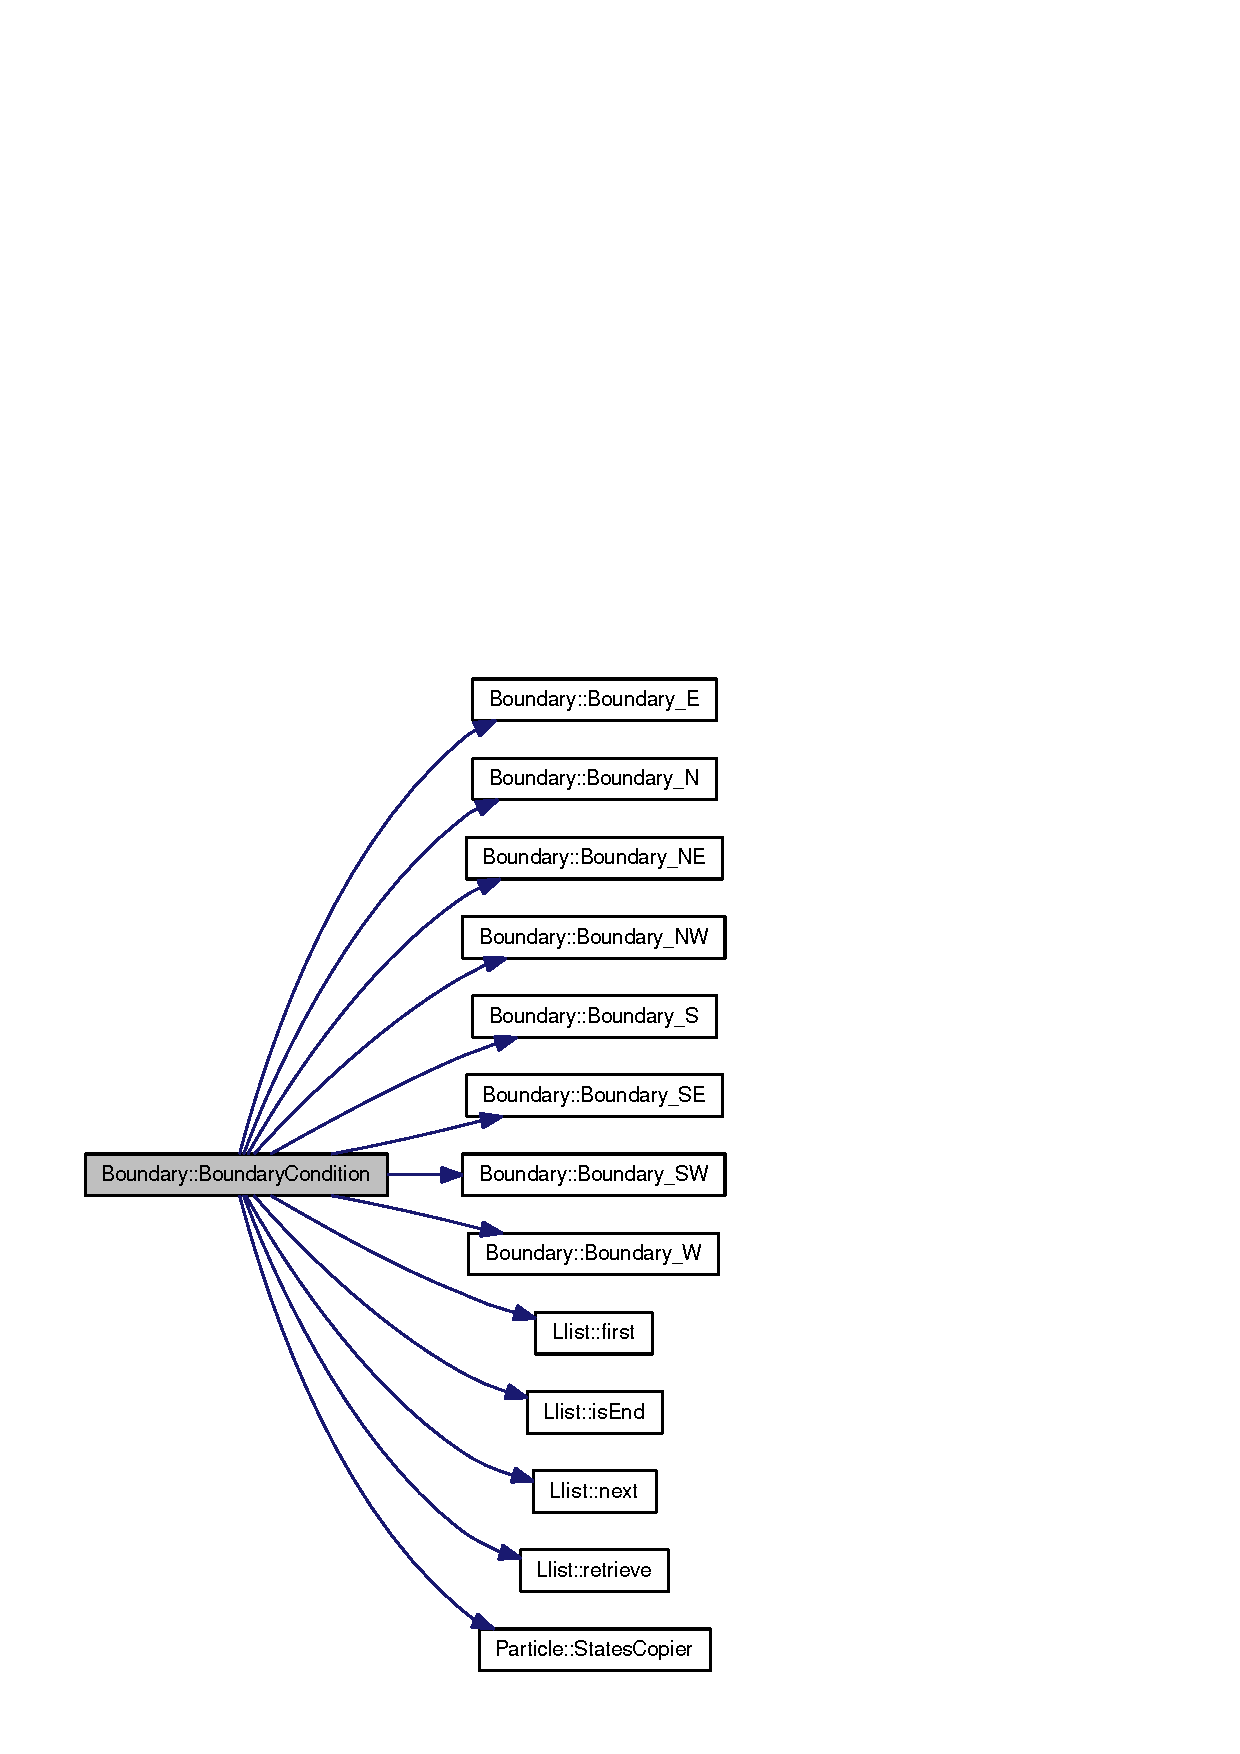
\includegraphics[width=176pt]{classBoundary_bedd190ee91482e4e59b2a613ab25d57_cgraph}
\end{center}
\end{figure}


Here is the caller graph for this function:\nopagebreak
\begin{figure}[H]
\begin{center}
\leavevmode
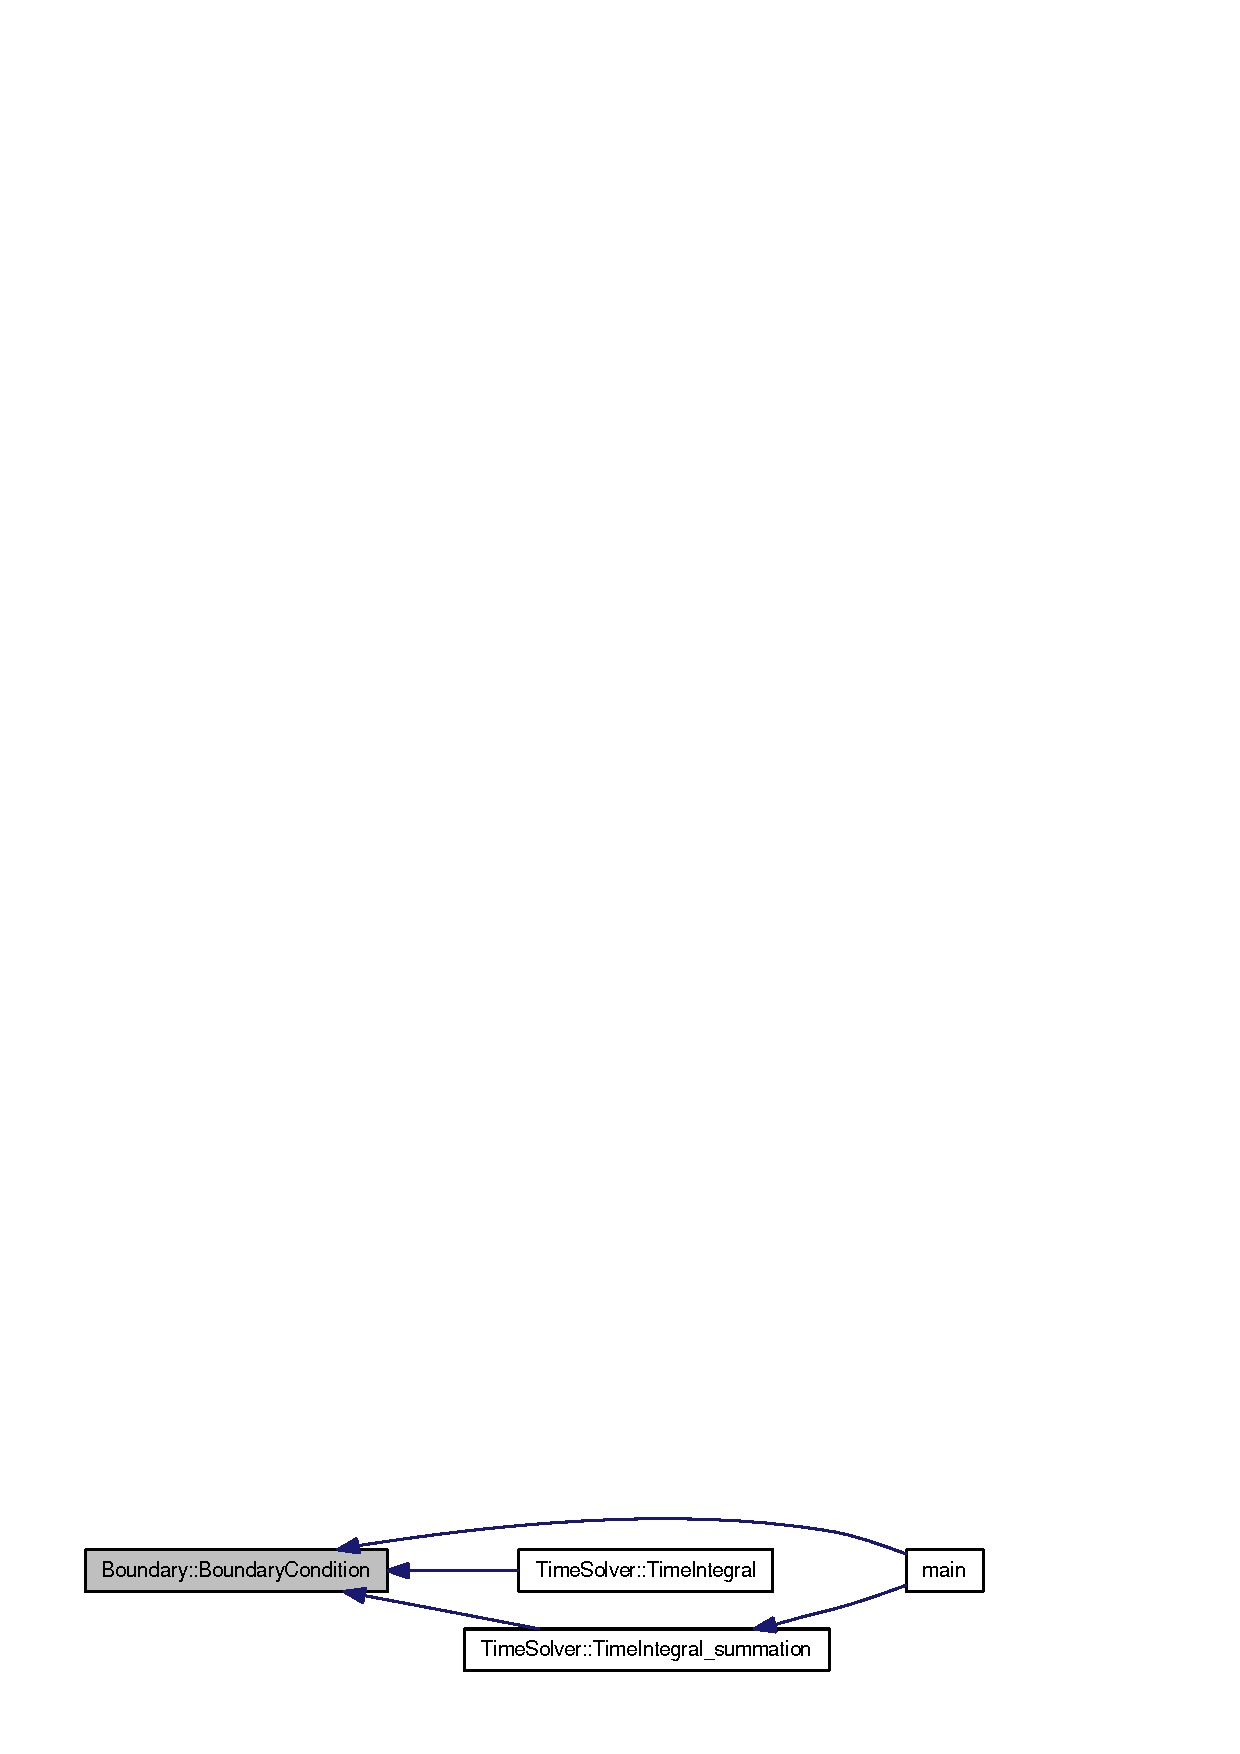
\includegraphics[width=238pt]{classBoundary_bedd190ee91482e4e59b2a613ab25d57_icgraph}
\end{center}
\end{figure}
\hypertarget{classBoundary_8a40f99b73f3622cd5f1387fcbbdb824}{
\index{Boundary@{Boundary}!BuildBoundaryParticles@{BuildBoundaryParticles}}
\index{BuildBoundaryParticles@{BuildBoundaryParticles}!Boundary@{Boundary}}
\subsubsection[{BuildBoundaryParticles}]{\setlength{\rightskip}{0pt plus 5cm}void Boundary::BuildBoundaryParticles ({\bf ParticleManager} \& {\em particles}, \/  {\bf Hydrodynamics} \& {\em hydro})}}
\label{classBoundary_8a40f99b73f3622cd5f1387fcbbdb824}


build boundary particles 



\begin{itemize}
\item clear boundary particles list

\item boundary condition for each side

\begin{itemize}
\item west side: test boundary parameter for one of the following cases and then build the appropriate boundary particles

\begin{itemize}
\item the rigid wall conditions

\item the symmetry conditions

\item the perodic conditions \end{itemize}


\item east side

\begin{itemize}
\item the rigid wall conditions

\item the symmetry conditions

\item the perodic conditions\end{itemize}


\item south side

\begin{itemize}
\item the rigid wall conditions

\item the symmetry conditions

\item the perodic conditions\end{itemize}


\item north side

\begin{itemize}
\item the rigid wall conditions

\item the symmetry conditions

\item the perodic conditions\end{itemize}
\end{itemize}


\item considering the coner cells

\begin{itemize}
\item south-west corner \begin{itemize}
\item the rigid wall conditions

\item the symmetry conditions

\item the perodic conditions \end{itemize}


\item north-west corner

\begin{itemize}
\item the rigid wall conditions

\item the symmetry conditions

\item the perodic conditions\end{itemize}


\item north-east corner

\begin{itemize}
\item the rigid wall conditions

\item the symmetry conditions

\item the perodic conditions\end{itemize}


\item south-east corner

\begin{itemize}
\item the rigid wall conditions

\item the symmetry conditions

\item the perodic conditions\end{itemize}
\end{itemize}
\end{itemize}


Here is the call graph for this function:\nopagebreak
\begin{figure}[H]
\begin{center}
\leavevmode
\includegraphics[width=186pt]{classBoundary_8a40f99b73f3622cd5f1387fcbbdb824_cgraph}
\end{center}
\end{figure}


Here is the caller graph for this function:\nopagebreak
\begin{figure}[H]
\begin{center}
\leavevmode
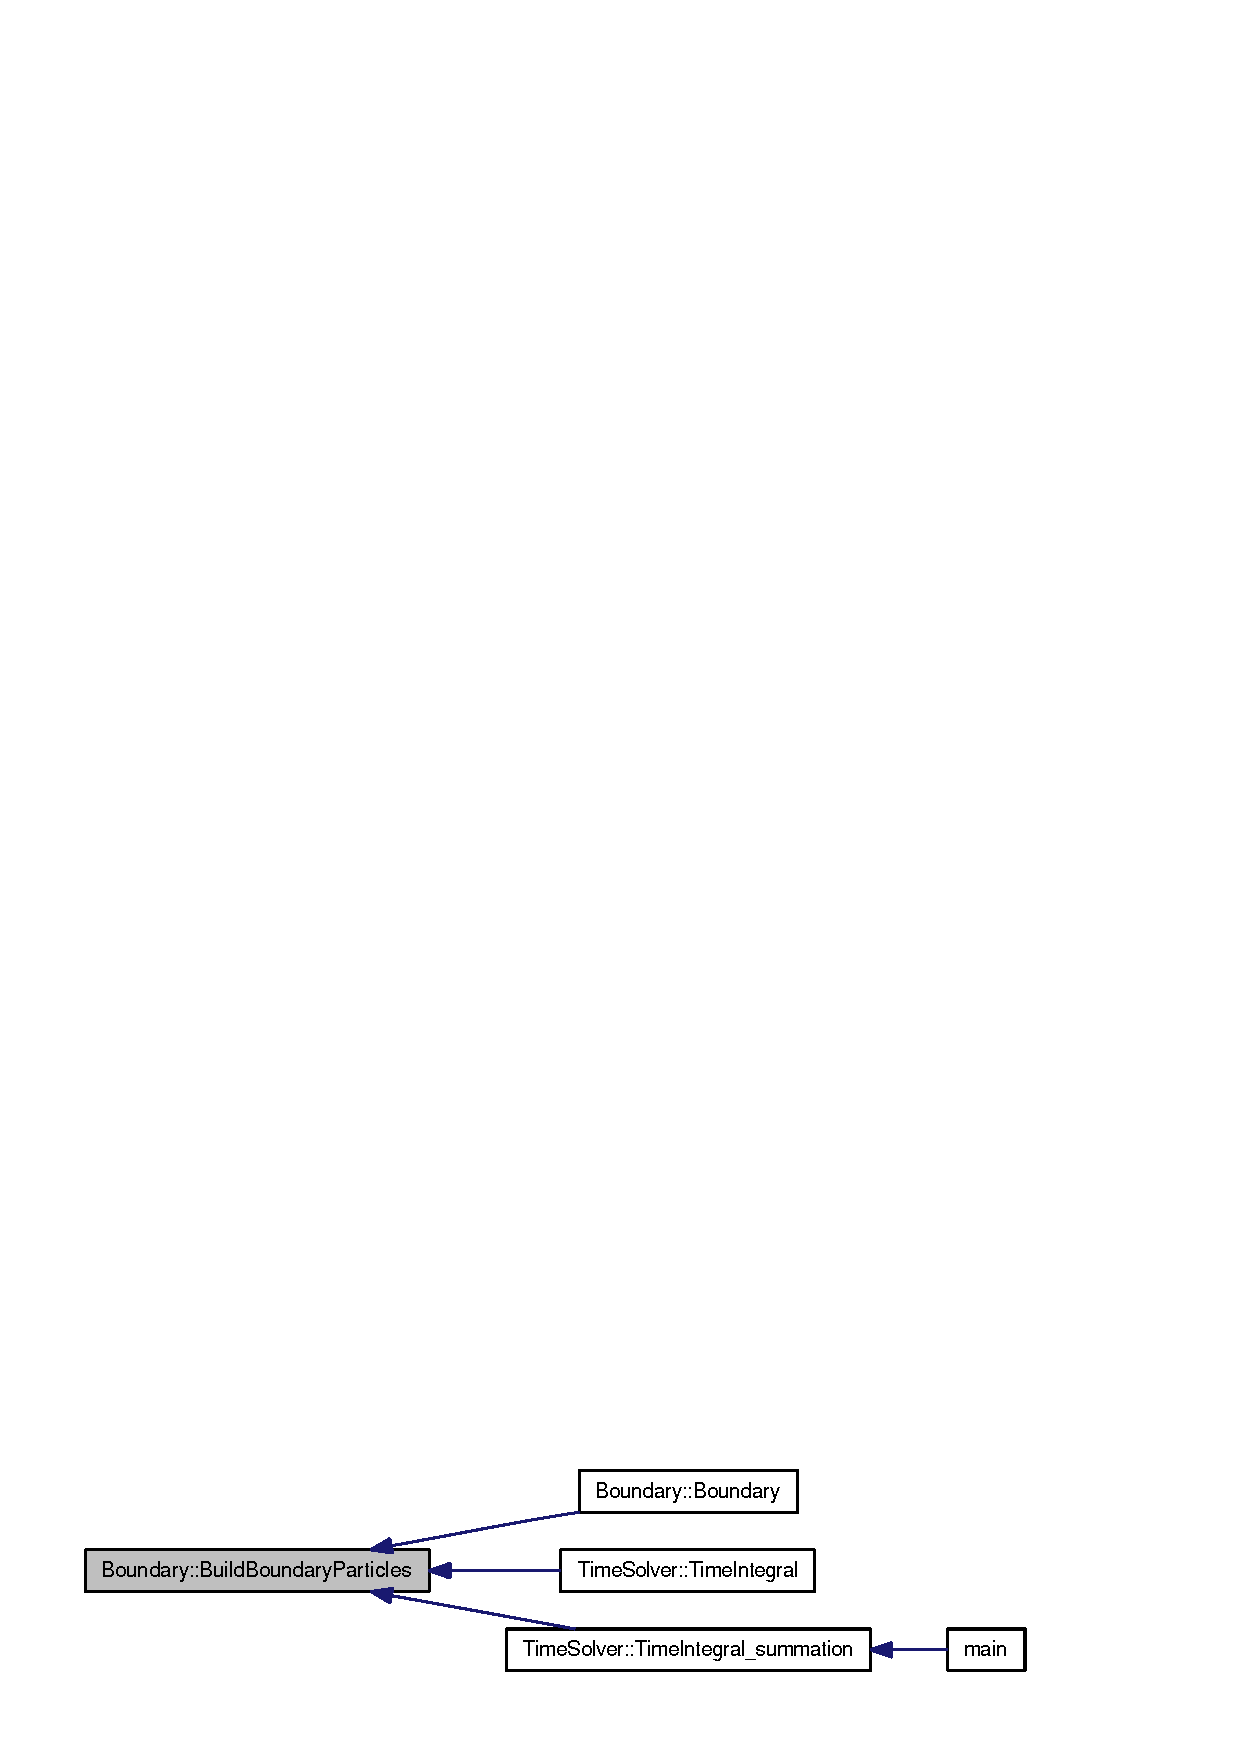
\includegraphics[width=248pt]{classBoundary_8a40f99b73f3622cd5f1387fcbbdb824_icgraph}
\end{center}
\end{figure}
\hypertarget{classBoundary_ac37e18aaf60503a66173d9428ed9e54}{
\index{Boundary@{Boundary}!RunAwayCheck@{RunAwayCheck}}
\index{RunAwayCheck@{RunAwayCheck}!Boundary@{Boundary}}
\subsubsection[{RunAwayCheck}]{\setlength{\rightskip}{0pt plus 5cm}void Boundary::RunAwayCheck ({\bf Hydrodynamics} \& {\em hydro})}}
\label{classBoundary_ac37e18aaf60503a66173d9428ed9e54}


check particle if particle run out of the computational domain 



\begin{itemize}
\item iterate the partilce list\end{itemize}


\begin{itemize}
\item only checking real particles (for all boundaries) \end{itemize}


Here is the call graph for this function:\nopagebreak
\begin{figure}[H]
\begin{center}
\leavevmode
\includegraphics[width=142pt]{classBoundary_ac37e18aaf60503a66173d9428ed9e54_cgraph}
\end{center}
\end{figure}


Here is the caller graph for this function:\nopagebreak
\begin{figure}[H]
\begin{center}
\leavevmode
\includegraphics[width=231pt]{classBoundary_ac37e18aaf60503a66173d9428ed9e54_icgraph}
\end{center}
\end{figure}
\hypertarget{classBoundary_116df4b717184d962f40bdc88de26763}{
\index{Boundary@{Boundary}!show\_\-information@{show\_\-information}}
\index{show\_\-information@{show\_\-information}!Boundary@{Boundary}}
\subsubsection[{show\_\-information}]{\setlength{\rightskip}{0pt plus 5cm}void Boundary::show\_\-information ({\bf Initiation} \& {\em ini})\hspace{0.3cm}{\tt  \mbox{[}private\mbox{]}}}}
\label{classBoundary_116df4b717184d962f40bdc88de26763}


show information on screen 



\begin{itemize}
\item output the property parameters to the screen \end{itemize}


Here is the caller graph for this function:\nopagebreak
\begin{figure}[H]
\begin{center}
\leavevmode
\includegraphics[width=162pt]{classBoundary_116df4b717184d962f40bdc88de26763_icgraph}
\end{center}
\end{figure}


\subsection{Member Data Documentation}
\hypertarget{classBoundary_10dd58ba0715412968c4902fe80b1318}{
\index{Boundary@{Boundary}!xBl@{xBl}}
\index{xBl@{xBl}!Boundary@{Boundary}}
\subsubsection[{xBl}]{\setlength{\rightskip}{0pt plus 5cm}int {\bf Boundary::xBl}}}
\label{classBoundary_10dd58ba0715412968c4902fe80b1318}


boundary condition indicator left hand side 

\begin{itemize}
\item 0: wall boundary condition\item 1: perodic boundary condition\item 2: free slip wall boundary condition\item 3: symmetry boundary condition \end{itemize}
\hypertarget{classBoundary_4a582b489cb580b8a6f3a7123f411a53}{
\index{Boundary@{Boundary}!xBr@{xBr}}
\index{xBr@{xBr}!Boundary@{Boundary}}
\subsubsection[{xBr}]{\setlength{\rightskip}{0pt plus 5cm}int {\bf Boundary::xBr}}}
\label{classBoundary_4a582b489cb580b8a6f3a7123f411a53}


boundary condition indicator right hand side 

\begin{itemize}
\item 0: wall boundary condition\item 1: perodic boundary condition\item 2: free slip wall boundary condition\item 3: symmetry boundary condition \end{itemize}
\hypertarget{classBoundary_0329bf6b954b3001418391cc16a9194e}{
\index{Boundary@{Boundary}!yBd@{yBd}}
\index{yBd@{yBd}!Boundary@{Boundary}}
\subsubsection[{yBd}]{\setlength{\rightskip}{0pt plus 5cm}int {\bf Boundary::yBd}}}
\label{classBoundary_0329bf6b954b3001418391cc16a9194e}


boundary condition indicator bottom side 

\begin{itemize}
\item 0: wall boundary condition\item 1: perodic boundary condition\item 2: free slip wall boundary condition\item 3: symmetry boundary condition \end{itemize}
\hypertarget{classBoundary_6ccff2a8c5a10104d202504034af9e84}{
\index{Boundary@{Boundary}!yBu@{yBu}}
\index{yBu@{yBu}!Boundary@{Boundary}}
\subsubsection[{yBu}]{\setlength{\rightskip}{0pt plus 5cm}int {\bf Boundary::yBu}}}
\label{classBoundary_6ccff2a8c5a10104d202504034af9e84}


boundary condition indicator upper side 

\begin{itemize}
\item 0: wall boundary condition\item 1: perodic boundary condition\item 2: free slip wall boundary condition\item 3: symmetry boundary condition \end{itemize}


The documentation for this class was generated from the following files:\begin{CompactItemize}
\item 
\hyperlink{boundary_8h}{boundary.h}\item 
\hyperlink{boundary_8cpp}{boundary.cpp}\end{CompactItemize}

\hypertarget{classDiagnose}{
\section{Diagnose Class Reference}
\label{classDiagnose}\index{Diagnose@{Diagnose}}
}
\hyperlink{classOutput}{Output} diagnosal.  


{\tt \#include $<$diagnose.h$>$}

Collaboration diagram for Diagnose:\nopagebreak
\begin{figure}[H]
\begin{center}
\leavevmode
\includegraphics[width=183pt]{classDiagnose__coll__graph}
\end{center}
\end{figure}
\subsection*{Public Member Functions}
\begin{CompactItemize}
\item 
\hyperlink{classDiagnose_915a3d571504c843748bf5e9a9ec801c}{Diagnose} (\hyperlink{classInitiation}{Initiation} \&ini, \hyperlink{classHydrodynamics}{Hydrodynamics} \&hydro)
\begin{CompactList}\small\item\em constructor \item\end{CompactList}\item 
void \hyperlink{classDiagnose_bf6d65f3716a9d637186f97c62f7218b}{SaveStates} (\hyperlink{classHydrodynamics}{Hydrodynamics} \&hydro)
\begin{CompactList}\small\item\em save the states of a particle in particle states vectors (vx\_\-list, vy\_\-list, rho\_\-list) \item\end{CompactList}\item 
void \hyperlink{classDiagnose_db2f9991031fb8c301f44518c1d851ea}{OutputProfile} (double Time, \hyperlink{classInitiation}{Initiation} \&ini)
\begin{CompactList}\small\item\em output distribution up to the time \item\end{CompactList}\item 
void \hyperlink{classDiagnose_8c14b3fa58083f64be2018bd0462604d}{Average} (\hyperlink{classParticleManager}{ParticleManager} \&particles, \hyperlink{classMLS}{MLS} \&mls, \hyperlink{classQuinticSpline}{QuinticSpline} \&weight\_\-function, \hyperlink{classInitiation}{Initiation} \&ini)
\begin{CompactList}\small\item\em calculate the average values \item\end{CompactList}\item 
void \hyperlink{classDiagnose_dc46dd26362f94e09b956b3affa247c9}{OutputAverage} (double Time, \hyperlink{classInitiation}{Initiation} \&ini)
\begin{CompactList}\small\item\em output the average values \item\end{CompactList}\item 
void \hyperlink{classDiagnose_9c73b32dc8facce488617780250c14bf}{KineticInformation} (double Time, \hyperlink{classInitiation}{Initiation} \&ini, \hyperlink{classHydrodynamics}{Hydrodynamics} \&hydro)
\begin{CompactList}\small\item\em track the globle average kinetic energy, weight center position and velocity \item\end{CompactList}\end{CompactItemize}
\subsection*{Private Member Functions}
\begin{CompactItemize}
\item 
\hypertarget{classDiagnose_ef3922caa185f5d587edad0eaaf655d3}{
void \hyperlink{classDiagnose_ef3922caa185f5d587edad0eaaf655d3}{BuildDistribution} (\hyperlink{classLlist}{Llist}$<$ double $>$ \&list, double dstrb\mbox{[}2\mbox{]}\mbox{[}101\mbox{]})}
\label{classDiagnose_ef3922caa185f5d587edad0eaaf655d3}

\begin{CompactList}\small\item\em build distribution \item\end{CompactList}\end{CompactItemize}
\subsection*{Private Attributes}
\begin{CompactItemize}
\item 
\hypertarget{classDiagnose_ff5505506d498c9a3d41a15b848f4fed}{
double \hyperlink{classDiagnose_ff5505506d498c9a3d41a15b848f4fed}{delta}}
\label{classDiagnose_ff5505506d498c9a3d41a15b848f4fed}

\begin{CompactList}\small\item\em the inital particle distance \item\end{CompactList}\item 
\hypertarget{classDiagnose_392e23f84c8d6c19a62ff729dabc4b08}{
int \hyperlink{classDiagnose_392e23f84c8d6c19a62ff729dabc4b08}{x\_\-cells}}
\label{classDiagnose_392e23f84c8d6c19a62ff729dabc4b08}

\begin{CompactList}\small\item\em cells matrix for real particles \item\end{CompactList}\item 
\hypertarget{classDiagnose_b99ebe8786c68b5ef9477c49e32227ad}{
int \textbf{y\_\-cells}}
\label{classDiagnose_b99ebe8786c68b5ef9477c49e32227ad}

\item 
\hypertarget{classDiagnose_85b126f2b079c38847e1b8a42fe39604}{
int \hyperlink{classDiagnose_85b126f2b079c38847e1b8a42fe39604}{hdelta}}
\label{classDiagnose_85b126f2b079c38847e1b8a42fe39604}

\begin{CompactList}\small\item\em the ration between smoothing length and inital particle distance \item\end{CompactList}\item 
\hypertarget{classDiagnose_ea27d34fbb662ee394b81802ddeca495}{
char \hyperlink{classDiagnose_ea27d34fbb662ee394b81802ddeca495}{Project\_\-name} \mbox{[}25\mbox{]}}
\label{classDiagnose_ea27d34fbb662ee394b81802ddeca495}

\begin{CompactList}\small\item\em the project name \item\end{CompactList}\item 
\hypertarget{classDiagnose_e91dcce776e5182100a0d813c7a490c9}{
int \textbf{number\_\-of\_\-materials}}
\label{classDiagnose_e91dcce776e5182100a0d813c7a490c9}

\item 
\hypertarget{classDiagnose_f67fdb70cb79df3d31d151630c63cef8}{
double \hyperlink{classDiagnose_f67fdb70cb79df3d31d151630c63cef8}{vx\_\-dstrb} \mbox{[}2\mbox{]}\mbox{[}101\mbox{]}}
\label{classDiagnose_f67fdb70cb79df3d31d151630c63cef8}

\begin{CompactList}\small\item\em x-velocity distribution \item\end{CompactList}\item 
\hypertarget{classDiagnose_0ec20a8f26b147df7f6dd74f054518fb}{
double \hyperlink{classDiagnose_0ec20a8f26b147df7f6dd74f054518fb}{vy\_\-dstrb} \mbox{[}2\mbox{]}\mbox{[}101\mbox{]}}
\label{classDiagnose_0ec20a8f26b147df7f6dd74f054518fb}

\begin{CompactList}\small\item\em y-velocity distribution \item\end{CompactList}\item 
\hypertarget{classDiagnose_c3b8eb576691e06bc18f30e1e23b053c}{
double \hyperlink{classDiagnose_c3b8eb576691e06bc18f30e1e23b053c}{rho\_\-dstrb} \mbox{[}2\mbox{]}\mbox{[}101\mbox{]}}
\label{classDiagnose_c3b8eb576691e06bc18f30e1e23b053c}

\begin{CompactList}\small\item\em density distribution \item\end{CompactList}\item 
\hypertarget{classDiagnose_145722f84ce6e10d9e6fc08104824996}{
\hyperlink{classLlist}{Llist}$<$ double $>$ \hyperlink{classDiagnose_145722f84ce6e10d9e6fc08104824996}{vx\_\-list}}
\label{classDiagnose_145722f84ce6e10d9e6fc08104824996}

\begin{CompactList}\small\item\em list for vx states of a given particle \item\end{CompactList}\item 
\hypertarget{classDiagnose_7b7a236d8ac6f9b7a901670a8f7703e0}{
\hyperlink{classLlist}{Llist}$<$ double $>$ \hyperlink{classDiagnose_7b7a236d8ac6f9b7a901670a8f7703e0}{vy\_\-list}}
\label{classDiagnose_7b7a236d8ac6f9b7a901670a8f7703e0}

\begin{CompactList}\small\item\em list for vy states of a given particle \item\end{CompactList}\item 
\hypertarget{classDiagnose_d10e7325edc977979a7db9fdcd34d8fd}{
\hyperlink{classLlist}{Llist}$<$ double $>$ \hyperlink{classDiagnose_d10e7325edc977979a7db9fdcd34d8fd}{rho\_\-list}}
\label{classDiagnose_d10e7325edc977979a7db9fdcd34d8fd}

\begin{CompactList}\small\item\em list for rho states of a given particle \item\end{CompactList}\item 
\hypertarget{classDiagnose_63dce0bdefd95c49730ab011321ad984}{
int \hyperlink{classDiagnose_63dce0bdefd95c49730ab011321ad984}{gridx}}
\label{classDiagnose_63dce0bdefd95c49730ab011321ad984}

\begin{CompactList}\small\item\em average profile mesh size in x-direction \item\end{CompactList}\item 
\hypertarget{classDiagnose_3cda015218278477cbbe85b6e55b4398}{
int \hyperlink{classDiagnose_3cda015218278477cbbe85b6e55b4398}{gridy}}
\label{classDiagnose_3cda015218278477cbbe85b6e55b4398}

\begin{CompactList}\small\item\em average profile mesh size in y-direction \item\end{CompactList}\item 
\hypertarget{classDiagnose_8fbc4859156ad72a70b471edd8326552}{
double $\ast$$\ast$$\ast$ \textbf{U}}
\label{classDiagnose_8fbc4859156ad72a70b471edd8326552}

\item 
\hypertarget{classDiagnose_a08ef64241663163214a68507d578e27}{
int \hyperlink{classDiagnose_a08ef64241663163214a68507d578e27}{n\_\-average}}
\label{classDiagnose_a08ef64241663163214a68507d578e27}

\begin{CompactList}\small\item\em the times of average \item\end{CompactList}\item 
double \hyperlink{classDiagnose_31e87c9b084b73a78c1e2758149800ed}{ttl\_\-m}
\begin{CompactList}\small\item\em total mass, global average kinetic energy, \item\end{CompactList}\item 
\hypertarget{classDiagnose_fb8a8b1acd170da00404455ee0e674df}{
double $\ast$ \hyperlink{classDiagnose_fb8a8b1acd170da00404455ee0e674df}{mtl\_\-m}}
\label{classDiagnose_fb8a8b1acd170da00404455ee0e674df}

\begin{CompactList}\small\item\em ??????{\bf (\hyperlink{diagnose_8h}{diagnose.h}, line 36)} \item\end{CompactList}\item 
\hypertarget{classDiagnose_1784f6a7677b271e8968147df019e8b0}{
double \hyperlink{classDiagnose_1784f6a7677b271e8968147df019e8b0}{glb\_\-ave\_\-Ek}}
\label{classDiagnose_1784f6a7677b271e8968147df019e8b0}

\begin{CompactList}\small\item\em global average kinetic energy \item\end{CompactList}\item 
\hypertarget{classDiagnose_52f9cc1859fecd569c05de78243e45bd}{
Vec2d $\ast$ \hyperlink{classDiagnose_52f9cc1859fecd569c05de78243e45bd}{wght\_\-cntr}}
\label{classDiagnose_52f9cc1859fecd569c05de78243e45bd}

\begin{CompactList}\small\item\em material weight center position \item\end{CompactList}\item 
\hypertarget{classDiagnose_8b02748469646274034f793aab57193b}{
Vec2d $\ast$ \hyperlink{classDiagnose_8b02748469646274034f793aab57193b}{wght\_\-v}}
\label{classDiagnose_8b02748469646274034f793aab57193b}

\begin{CompactList}\small\item\em material weight center velocity \item\end{CompactList}\end{CompactItemize}


\subsection{Detailed Description}
\hyperlink{classOutput}{Output} diagnosal. 

\subsection{Constructor \& Destructor Documentation}
\hypertarget{classDiagnose_915a3d571504c843748bf5e9a9ec801c}{
\index{Diagnose@{Diagnose}!Diagnose@{Diagnose}}
\index{Diagnose@{Diagnose}!Diagnose@{Diagnose}}
\subsubsection[{Diagnose}]{\setlength{\rightskip}{0pt plus 5cm}Diagnose::Diagnose ({\bf Initiation} \& {\em ini}, \/  {\bf Hydrodynamics} \& {\em hydro})}}
\label{classDiagnose_915a3d571504c843748bf5e9a9ec801c}


constructor 



\begin{itemize}
\item copy parameters from \hyperlink{classInitiation}{Initiation} class

\item copy boundary properties from initiation class

\item calculate total mass

\item produce output file name (\char`\"{}kinetic\_\-info.dat\char`\"{})and file header \end{itemize}


Here is the call graph for this function:\nopagebreak
\begin{figure}[H]
\begin{center}
\leavevmode
\includegraphics[width=128pt]{classDiagnose_915a3d571504c843748bf5e9a9ec801c_cgraph}
\end{center}
\end{figure}


\subsection{Member Function Documentation}
\hypertarget{classDiagnose_8c14b3fa58083f64be2018bd0462604d}{
\index{Diagnose@{Diagnose}!Average@{Average}}
\index{Average@{Average}!Diagnose@{Diagnose}}
\subsubsection[{Average}]{\setlength{\rightskip}{0pt plus 5cm}void Diagnose::Average ({\bf ParticleManager} \& {\em particles}, \/  {\bf MLS} \& {\em mls}, \/  {\bf QuinticSpline} \& {\em weight\_\-function}, \/  {\bf Initiation} \& {\em ini})}}
\label{classDiagnose_8c14b3fa58083f64be2018bd0462604d}


calculate the average values 



\begin{itemize}
\item loop the grid points

\begin{itemize}
\item build the NNP\_\-list

\item if the NNP list is not empty run \hyperlink{classMLS}{MLS} approximation

\item iterate this Nearest Neighbor \hyperlink{classParticle}{Particle} list

\begin{itemize}
\item get particle data \end{itemize}


\item clear the NNP\_\-list

\item calculating the averages \end{itemize}
\end{itemize}


Here is the call graph for this function:\nopagebreak
\begin{figure}[H]
\begin{center}
\leavevmode
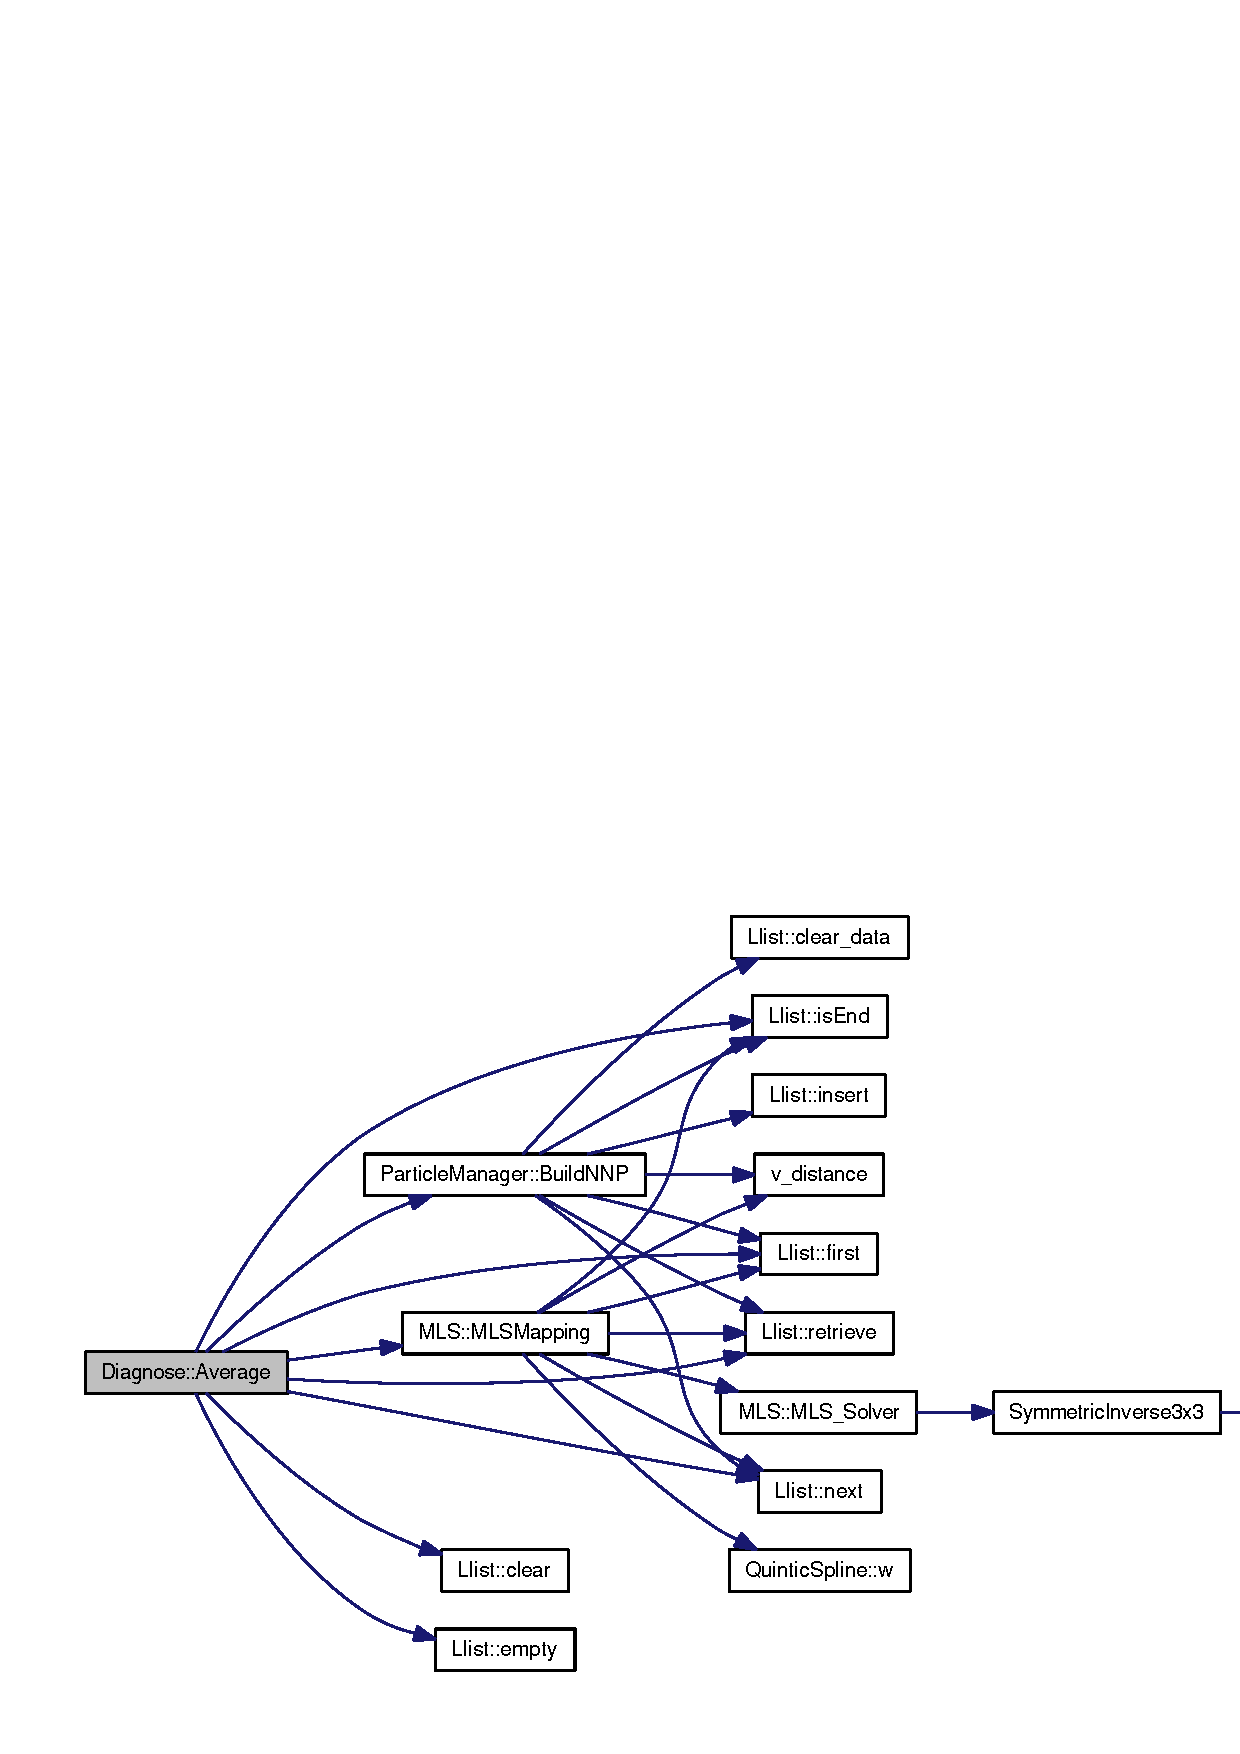
\includegraphics[width=331pt]{classDiagnose_8c14b3fa58083f64be2018bd0462604d_cgraph}
\end{center}
\end{figure}


Here is the caller graph for this function:\nopagebreak
\begin{figure}[H]
\begin{center}
\leavevmode
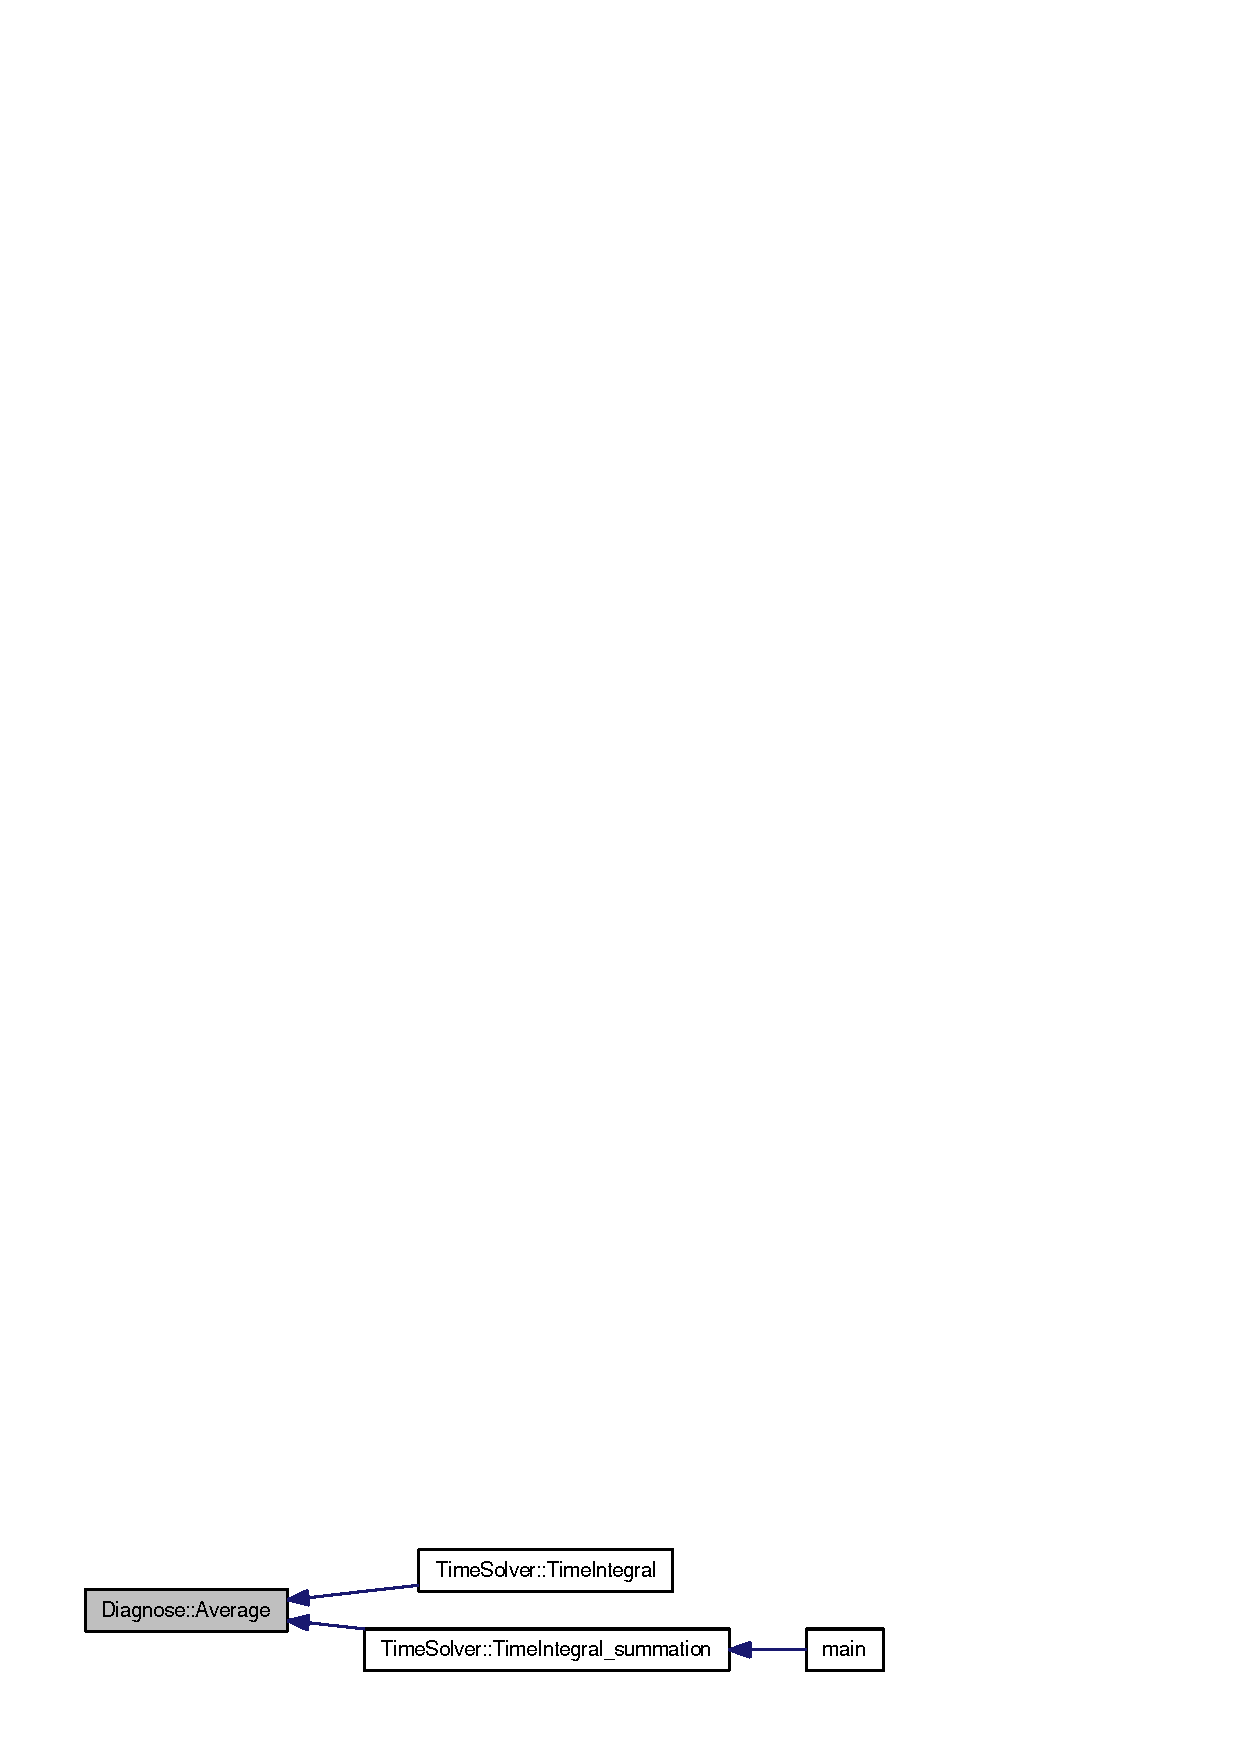
\includegraphics[width=214pt]{classDiagnose_8c14b3fa58083f64be2018bd0462604d_icgraph}
\end{center}
\end{figure}
\hypertarget{classDiagnose_9c73b32dc8facce488617780250c14bf}{
\index{Diagnose@{Diagnose}!KineticInformation@{KineticInformation}}
\index{KineticInformation@{KineticInformation}!Diagnose@{Diagnose}}
\subsubsection[{KineticInformation}]{\setlength{\rightskip}{0pt plus 5cm}void Diagnose::KineticInformation (double {\em Time}, \/  {\bf Initiation} \& {\em ini}, \/  {\bf Hydrodynamics} \& {\em hydro})}}
\label{classDiagnose_9c73b32dc8facce488617780250c14bf}


track the globle average kinetic energy, weight center position and velocity 



\begin{itemize}
\item produce output file name

\item iterate the partilce list and calculate data

\item output calculated data in \char`\"{}kinetic\_\-info.dat\char`\"{} \end{itemize}


Here is the call graph for this function:\nopagebreak
\begin{figure}[H]
\begin{center}
\leavevmode
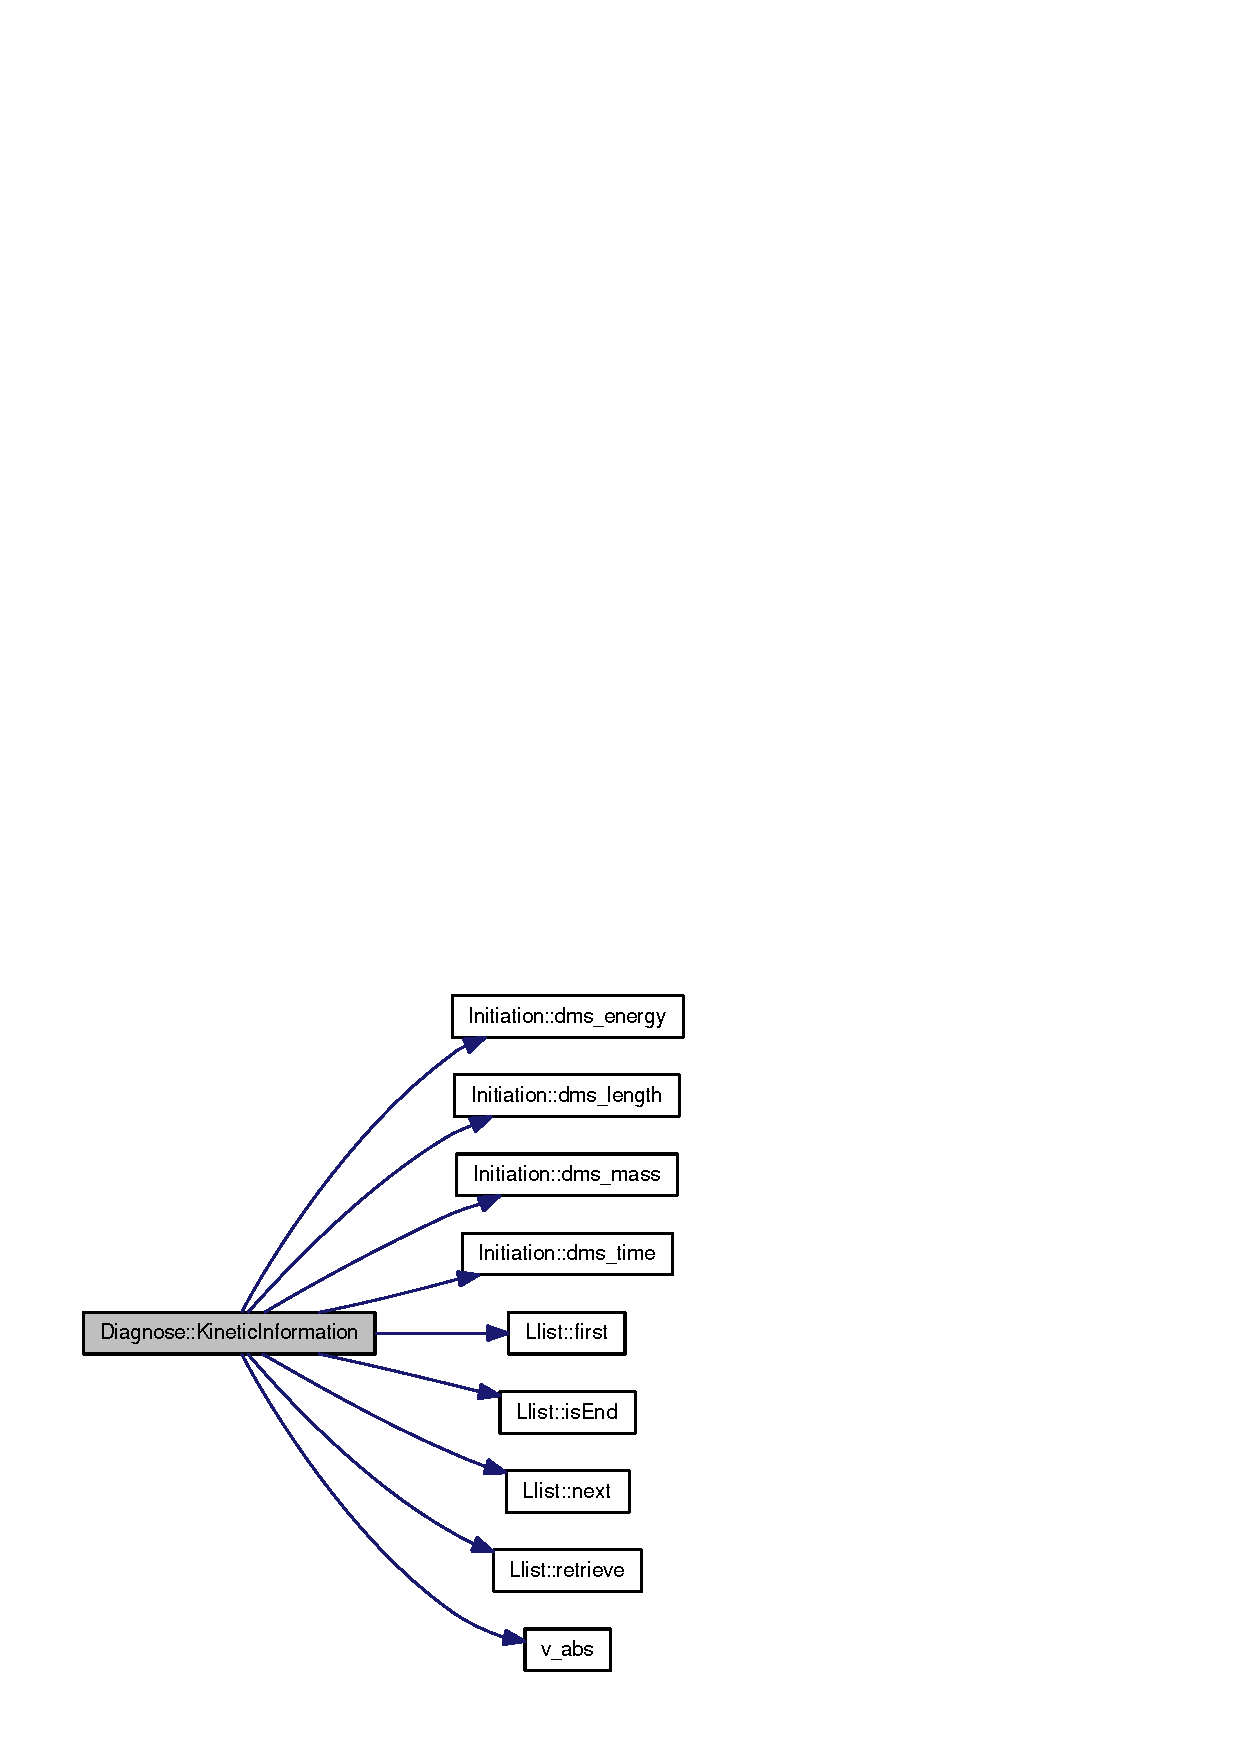
\includegraphics[width=166pt]{classDiagnose_9c73b32dc8facce488617780250c14bf_cgraph}
\end{center}
\end{figure}


Here is the caller graph for this function:\nopagebreak
\begin{figure}[H]
\begin{center}
\leavevmode
\includegraphics[width=235pt]{classDiagnose_9c73b32dc8facce488617780250c14bf_icgraph}
\end{center}
\end{figure}
\hypertarget{classDiagnose_dc46dd26362f94e09b956b3affa247c9}{
\index{Diagnose@{Diagnose}!OutputAverage@{OutputAverage}}
\index{OutputAverage@{OutputAverage}!Diagnose@{Diagnose}}
\subsubsection[{OutputAverage}]{\setlength{\rightskip}{0pt plus 5cm}void Diagnose::OutputAverage (double {\em Time}, \/  {\bf Initiation} \& {\em ini})}}
\label{classDiagnose_dc46dd26362f94e09b956b3affa247c9}


output the average values 



\begin{itemize}
\item produce output file name\end{itemize}


\begin{itemize}
\item defining header for tecplot(plot software)\end{itemize}


\begin{itemize}
\item loop the grid points and output data \end{itemize}


Here is the call graph for this function:\nopagebreak
\begin{figure}[H]
\begin{center}
\leavevmode
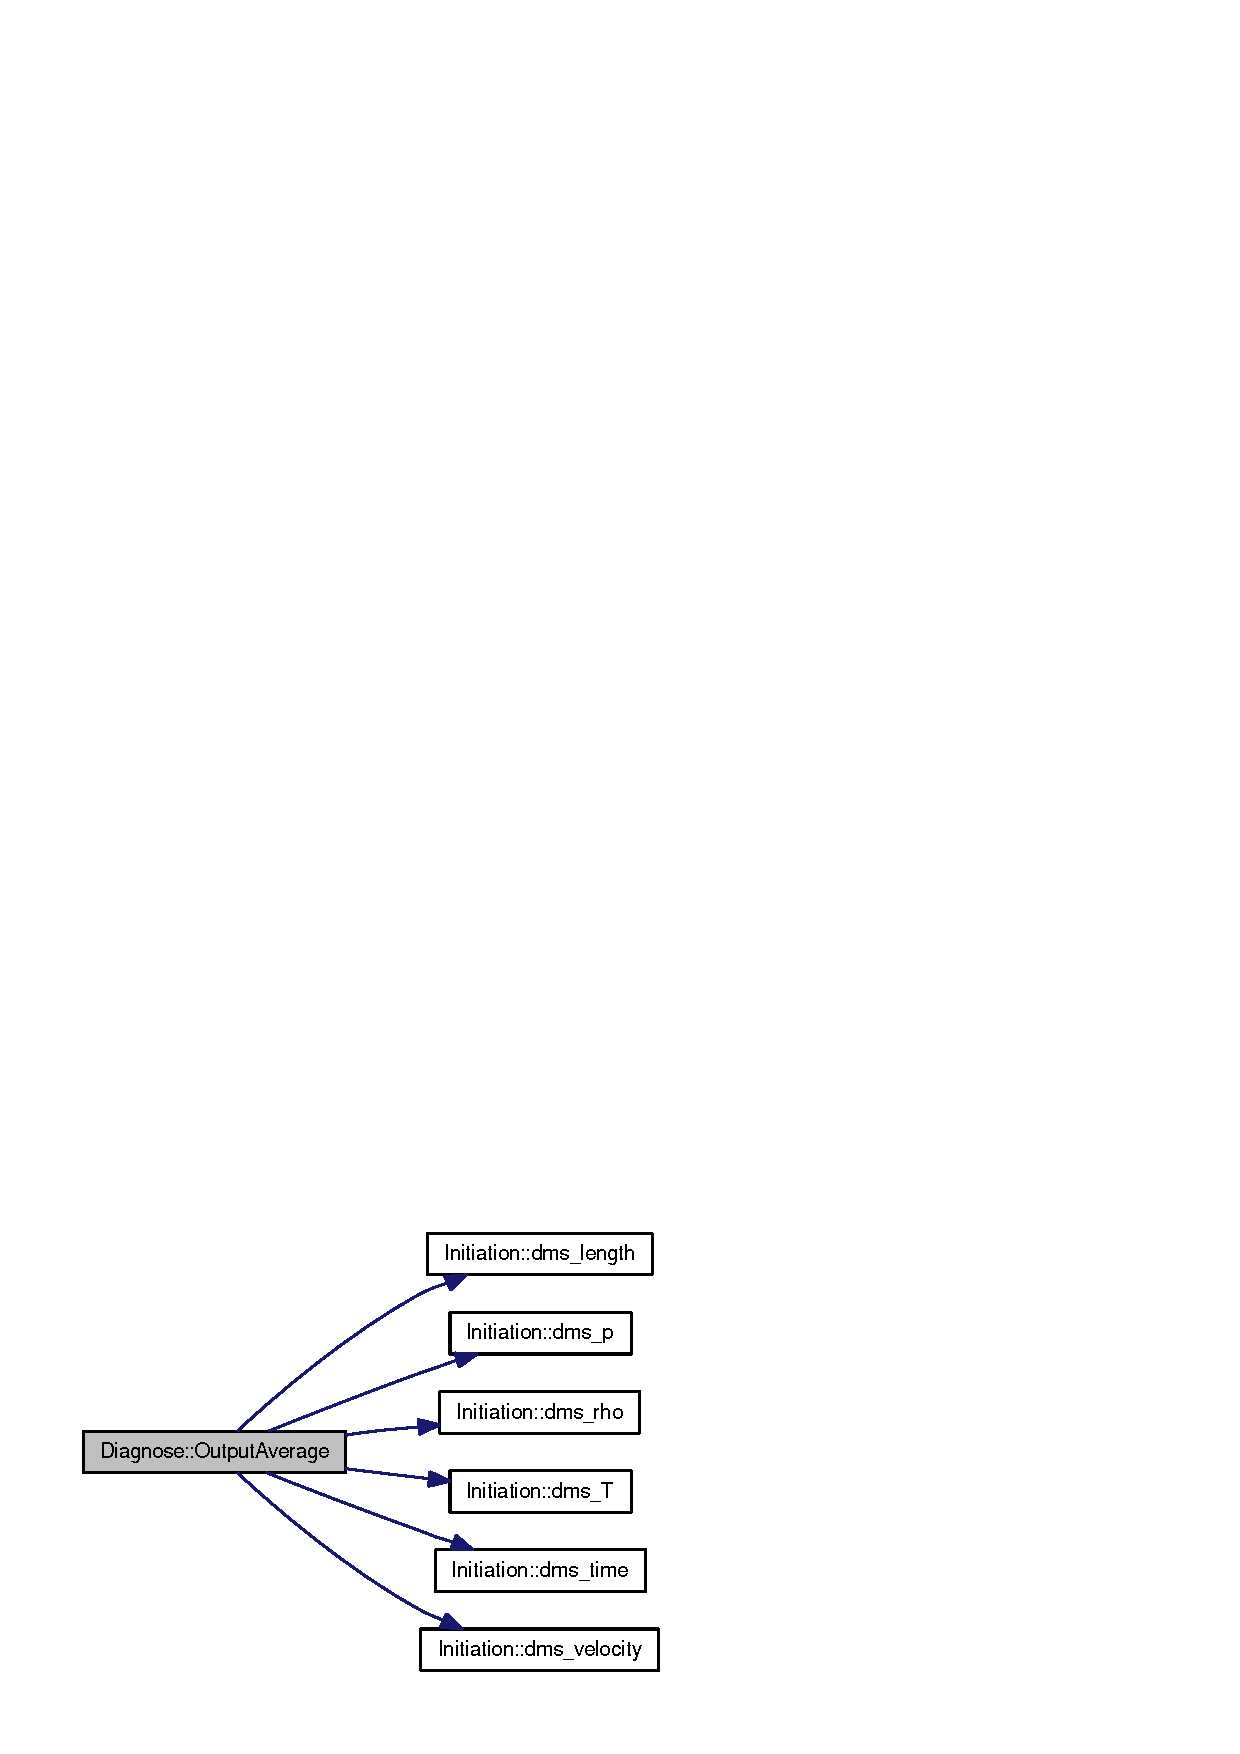
\includegraphics[width=160pt]{classDiagnose_dc46dd26362f94e09b956b3affa247c9_cgraph}
\end{center}
\end{figure}


Here is the caller graph for this function:\nopagebreak
\begin{figure}[H]
\begin{center}
\leavevmode
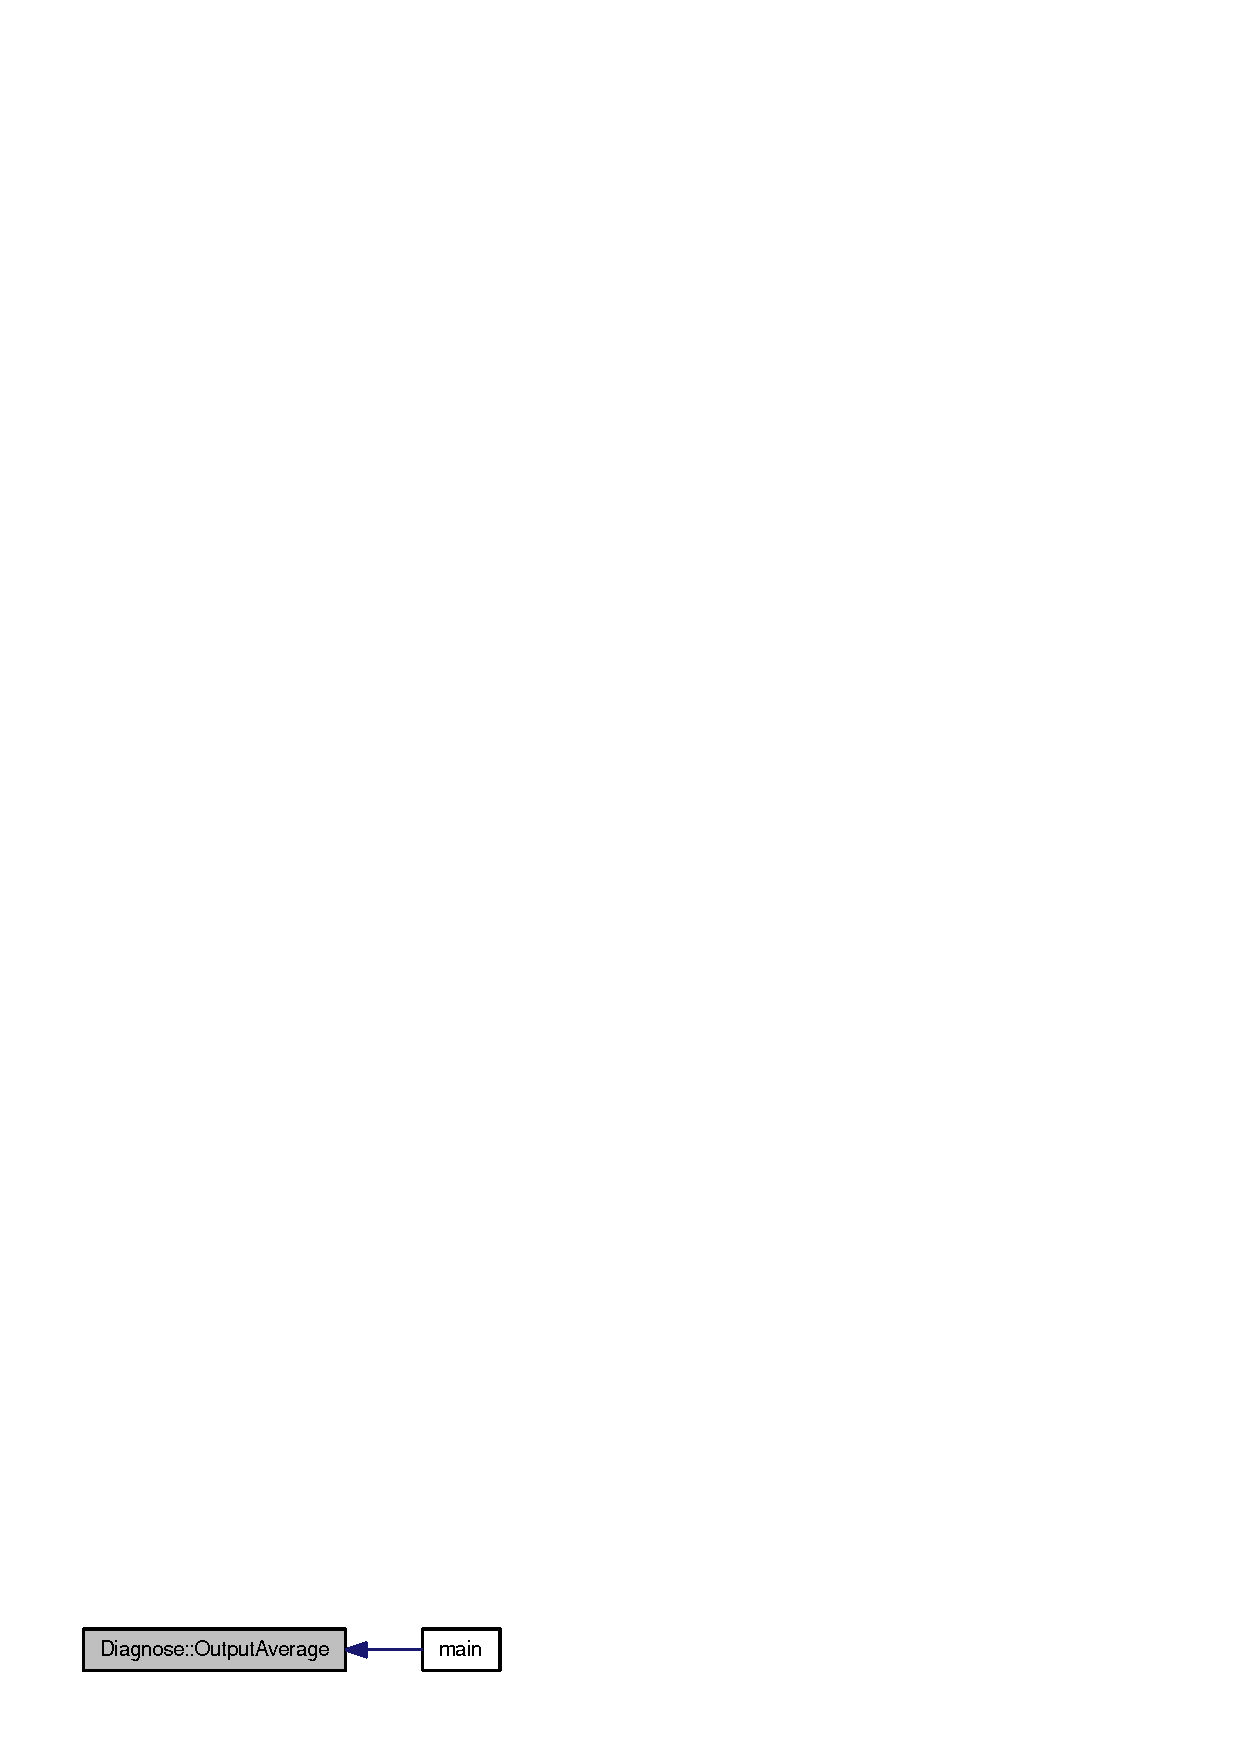
\includegraphics[width=122pt]{classDiagnose_dc46dd26362f94e09b956b3affa247c9_icgraph}
\end{center}
\end{figure}
\hypertarget{classDiagnose_db2f9991031fb8c301f44518c1d851ea}{
\index{Diagnose@{Diagnose}!OutputProfile@{OutputProfile}}
\index{OutputProfile@{OutputProfile}!Diagnose@{Diagnose}}
\subsubsection[{OutputProfile}]{\setlength{\rightskip}{0pt plus 5cm}void Diagnose::OutputProfile (double {\em Time}, \/  {\bf Initiation} \& {\em ini})}}
\label{classDiagnose_db2f9991031fb8c301f44518c1d851ea}


output distribution up to the time 



\begin{itemize}
\item produce output file name \char`\"{}dstrXXXX.dat\char`\"{}\end{itemize}


\begin{itemize}
\item defining file header for tecplot(plot software)\end{itemize}


-build the distribution

\begin{itemize}
\item normalize to unit\end{itemize}


\begin{itemize}
\item output distribution in file \end{itemize}


Here is the call graph for this function:\nopagebreak
\begin{figure}[H]
\begin{center}
\leavevmode
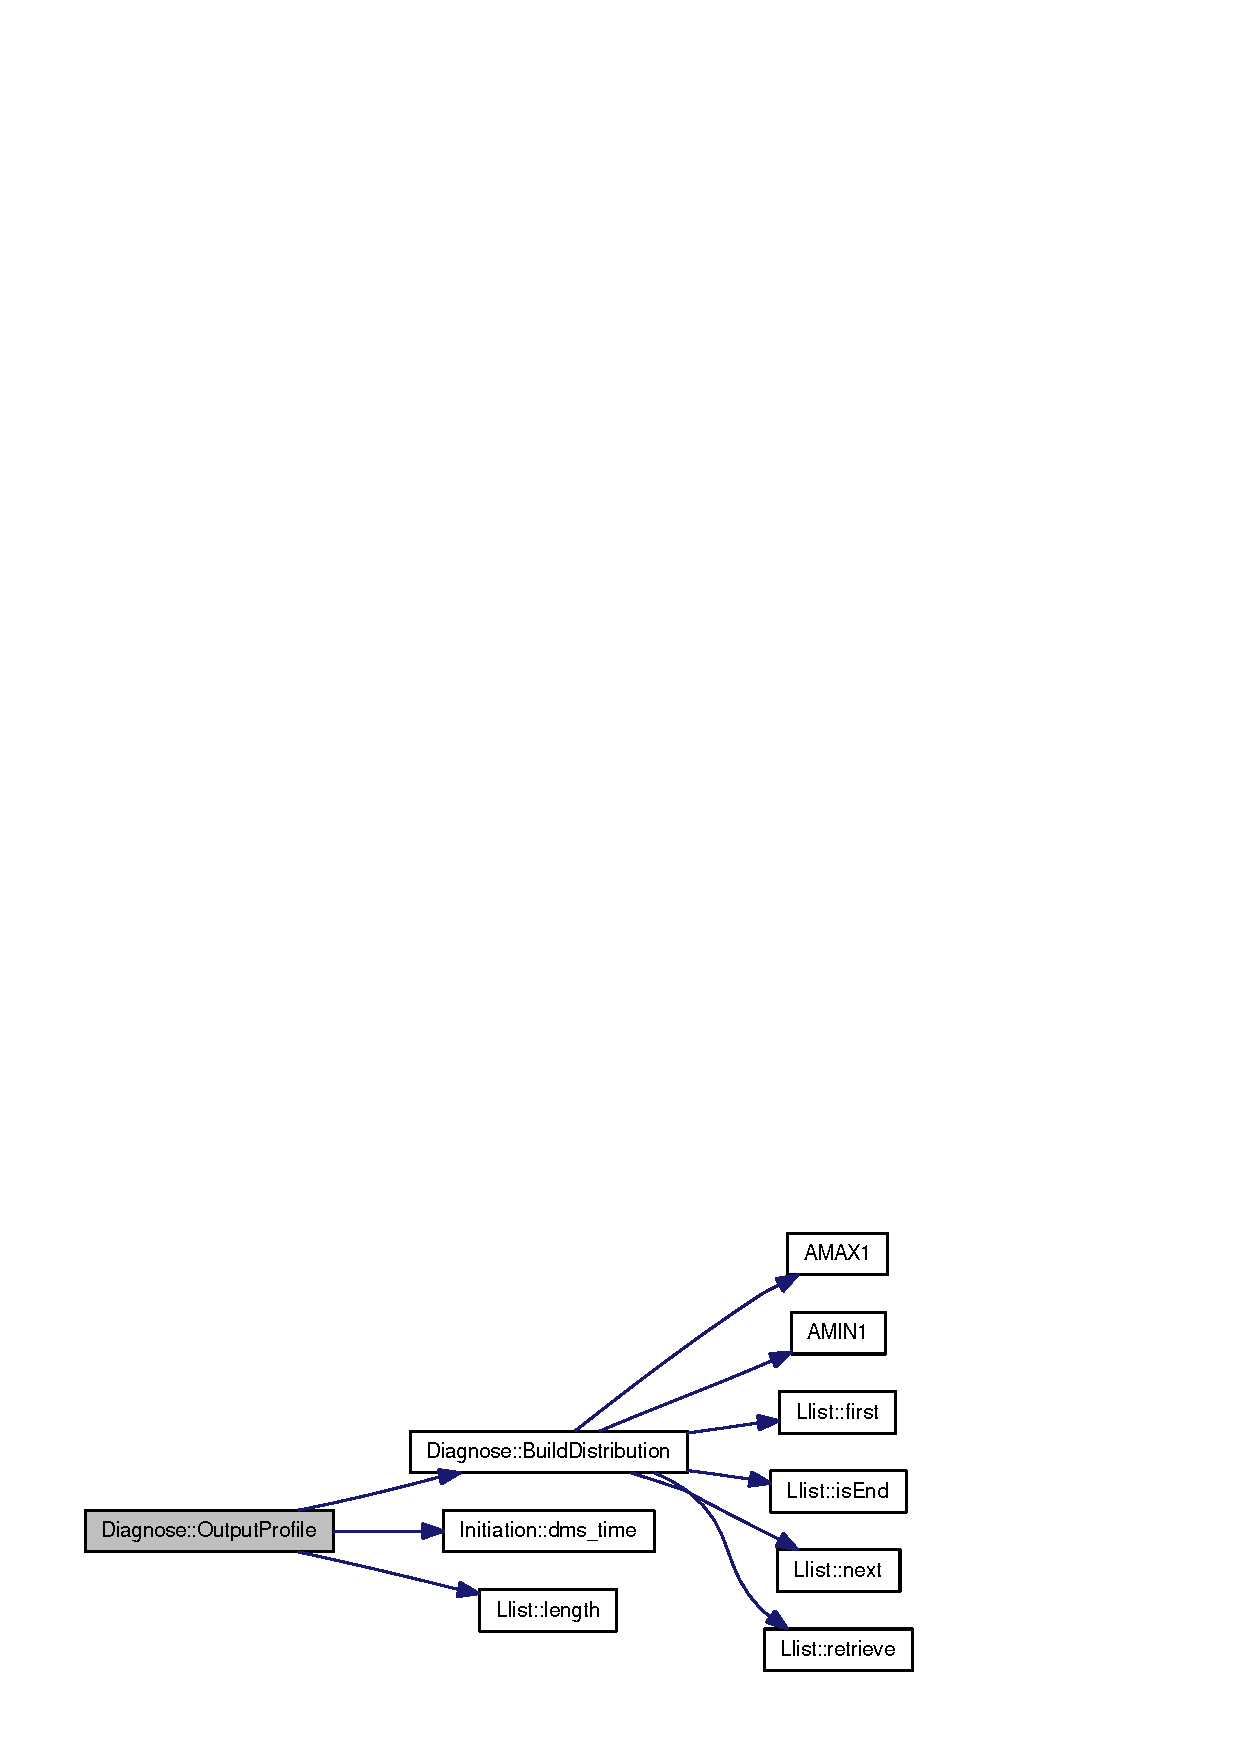
\includegraphics[width=221pt]{classDiagnose_db2f9991031fb8c301f44518c1d851ea_cgraph}
\end{center}
\end{figure}


Here is the caller graph for this function:\nopagebreak
\begin{figure}[H]
\begin{center}
\leavevmode
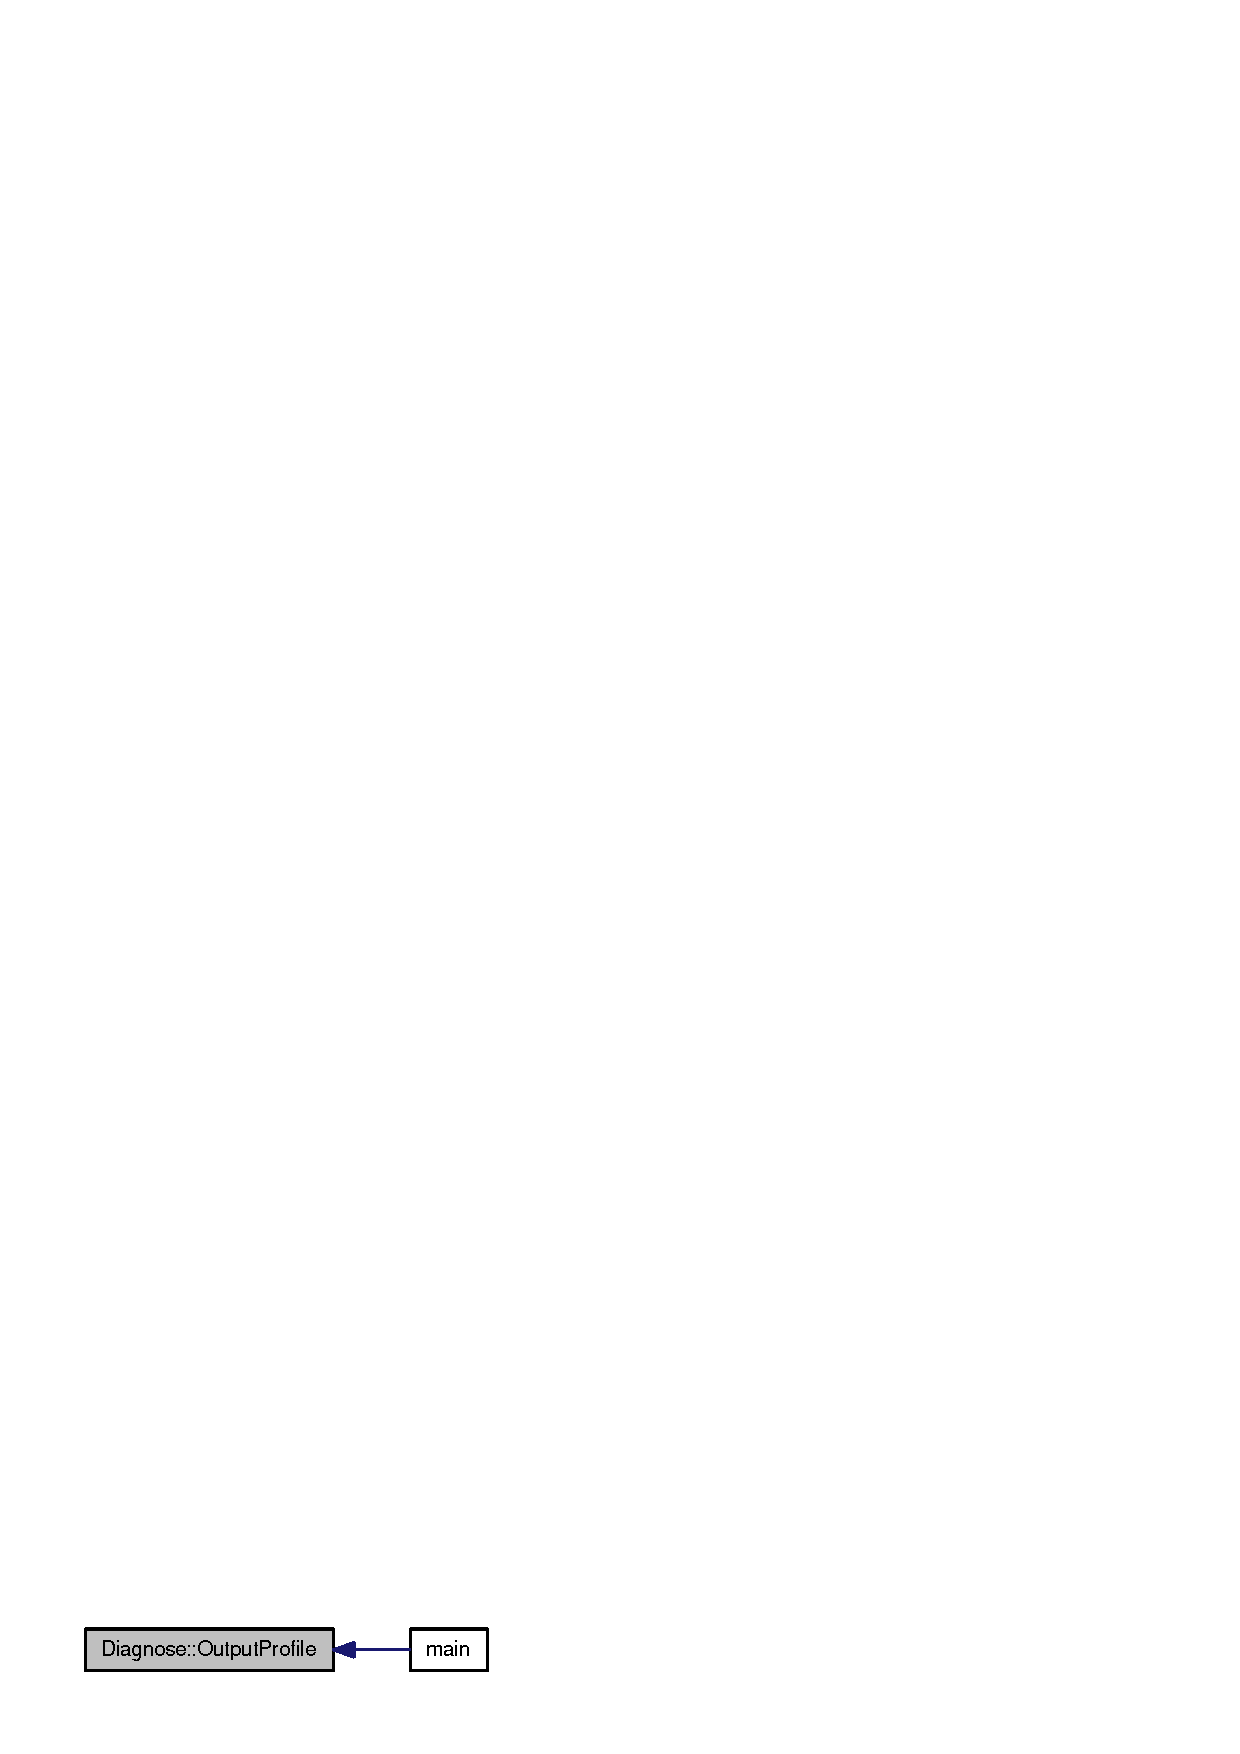
\includegraphics[width=119pt]{classDiagnose_db2f9991031fb8c301f44518c1d851ea_icgraph}
\end{center}
\end{figure}
\hypertarget{classDiagnose_bf6d65f3716a9d637186f97c62f7218b}{
\index{Diagnose@{Diagnose}!SaveStates@{SaveStates}}
\index{SaveStates@{SaveStates}!Diagnose@{Diagnose}}
\subsubsection[{SaveStates}]{\setlength{\rightskip}{0pt plus 5cm}void Diagnose::SaveStates ({\bf Hydrodynamics} \& {\em hydro})}}
\label{classDiagnose_bf6d65f3716a9d637186f97c62f7218b}


save the states of a particle in particle states vectors (vx\_\-list, vy\_\-list, rho\_\-list) 



\begin{itemize}
\item select a given node on the particle list\end{itemize}


\begin{itemize}
\item Insert the states of the particles in the states vectores (vx\_\-list, vy\_\-list, rho\_\-list) \end{itemize}


Here is the call graph for this function:\nopagebreak
\begin{figure}[H]
\begin{center}
\leavevmode
\includegraphics[width=132pt]{classDiagnose_bf6d65f3716a9d637186f97c62f7218b_cgraph}
\end{center}
\end{figure}


Here is the caller graph for this function:\nopagebreak
\begin{figure}[H]
\begin{center}
\leavevmode
\includegraphics[width=221pt]{classDiagnose_bf6d65f3716a9d637186f97c62f7218b_icgraph}
\end{center}
\end{figure}


\subsection{Member Data Documentation}
\hypertarget{classDiagnose_31e87c9b084b73a78c1e2758149800ed}{
\index{Diagnose@{Diagnose}!ttl\_\-m@{ttl\_\-m}}
\index{ttl\_\-m@{ttl\_\-m}!Diagnose@{Diagnose}}
\subsubsection[{ttl\_\-m}]{\setlength{\rightskip}{0pt plus 5cm}double {\bf Diagnose::ttl\_\-m}\hspace{0.3cm}{\tt  \mbox{[}private\mbox{]}}}}
\label{classDiagnose_31e87c9b084b73a78c1e2758149800ed}


total mass, global average kinetic energy, 

total mass 

The documentation for this class was generated from the following files:\begin{CompactItemize}
\item 
\hyperlink{diagnose_8h}{diagnose.h}\item 
\hyperlink{diagose_8cpp}{diagose.cpp}\end{CompactItemize}

\hypertarget{classForce}{
\section{Force Class Reference}
\label{classForce}\index{Force@{Force}}
}
The class defining force on or between particles.  


{\tt \#include $<$force.h$>$}

\subsection*{Public Member Functions}
\begin{CompactItemize}
\item 
\hyperlink{classForce_00983e3bbc206a00bb9253deafc4e424}{Force} ()
\begin{CompactList}\small\item\em shear and bulk slip length \item\end{CompactList}\item 
\hypertarget{classForce_6ce6bddb4bbe52af88b12827324a818d}{
\textbf{Force} (\hyperlink{classInitiation}{Initiation} \&ini)}
\label{classForce_6ce6bddb4bbe52af88b12827324a818d}

\item 
\hypertarget{classForce_75f2e675a6d57e08127d47b6bc31d3d9}{
void \hyperlink{classForce_75f2e675a6d57e08127d47b6bc31d3d9}{non\_\-dimensionalize} (\hyperlink{classInitiation}{Initiation} \&ini)}
\label{classForce_75f2e675a6d57e08127d47b6bc31d3d9}

\begin{CompactList}\small\item\em non-dimensionalize \item\end{CompactList}\end{CompactItemize}
\subsection*{Public Attributes}
\begin{CompactItemize}
\item 
\hypertarget{classForce_7142842359bf1e78499b5f59cff7a600}{
double \hyperlink{classForce_7142842359bf1e78499b5f59cff7a600}{sigma}}
\label{classForce_7142842359bf1e78499b5f59cff7a600}

\begin{CompactList}\small\item\em heat conduction slip length \item\end{CompactList}\item 
\hypertarget{classForce_5b371059110b1baee895f30c24e209f3}{
double \hyperlink{classForce_5b371059110b1baee895f30c24e209f3}{shear\_\-slip}}
\label{classForce_5b371059110b1baee895f30c24e209f3}

\begin{CompactList}\small\item\em surface tension parameters, its dimension is rho$\ast$u$^\wedge$2$\ast$L \item\end{CompactList}\item 
\hypertarget{classForce_707dd63d90d41bd1c0b345f5ba27a047}{
double \textbf{bulk\_\-slip}}
\label{classForce_707dd63d90d41bd1c0b345f5ba27a047}

\end{CompactItemize}
\subsection*{Private Attributes}
\begin{CompactItemize}
\item 
\hypertarget{classForce_ff0b02789964024867fd633fd0e5722a}{
double \hyperlink{classForce_ff0b02789964024867fd633fd0e5722a}{epsilon}}
\label{classForce_ff0b02789964024867fd633fd0e5722a}

\begin{CompactList}\small\item\em interactive force parameters \item\end{CompactList}\item 
\hypertarget{classForce_499d60a627ddd2b9a2909891cd45b78f}{
double \textbf{heat\_\-slip}}
\label{classForce_499d60a627ddd2b9a2909891cd45b78f}

\end{CompactItemize}
\subsection*{Static Private Attributes}
\begin{CompactItemize}
\item 
\hypertarget{classForce_84055a493186144b98ab363bd958095f}{
static int \hyperlink{classForce_84055a493186144b98ab363bd958095f}{number\_\-of\_\-materials} = 0}
\label{classForce_84055a493186144b98ab363bd958095f}

\begin{CompactList}\small\item\em total number of materials \item\end{CompactList}\item 
\hypertarget{classForce_bcab616ac69fe78d87567506dedd8a56}{
static double \hyperlink{classForce_bcab616ac69fe78d87567506dedd8a56}{smoothinglength} = 0.0}
\label{classForce_bcab616ac69fe78d87567506dedd8a56}

\begin{CompactList}\small\item\em smoothinglenth \item\end{CompactList}\end{CompactItemize}
\subsection*{Friends}
\begin{CompactItemize}
\item 
\hypertarget{classForce_652e6d35f07e2091db6c1d01e86e2286}{
class \hyperlink{classForce_652e6d35f07e2091db6c1d01e86e2286}{Hydrodynamics}}
\label{classForce_652e6d35f07e2091db6c1d01e86e2286}

\end{CompactItemize}


\subsection{Detailed Description}
The class defining force on or between particles. 

\subsection{Constructor \& Destructor Documentation}
\hypertarget{classForce_00983e3bbc206a00bb9253deafc4e424}{
\index{Force@{Force}!Force@{Force}}
\index{Force@{Force}!Force@{Force}}
\subsubsection[{Force}]{\setlength{\rightskip}{0pt plus 5cm}Force::Force ()}}
\label{classForce_00983e3bbc206a00bb9253deafc4e424}


shear and bulk slip length 

constructor 

The documentation for this class was generated from the following files:\begin{CompactItemize}
\item 
\hyperlink{force_8h}{force.h}\item 
force.cpp\end{CompactItemize}

\hypertarget{classHydrodynamics}{
\section{Hydrodynamics Class Reference}
\label{classHydrodynamics}\index{Hydrodynamics@{Hydrodynamics}}
}
Definition of materials and their hydrodynamical interactions.  


{\tt \#include $<$hydrodynamics.h$>$}

Collaboration diagram for Hydrodynamics:\nopagebreak
\begin{figure}[H]
\begin{center}
\leavevmode
\includegraphics[width=400pt]{classHydrodynamics__coll__graph}
\end{center}
\end{figure}
\subsection*{Public Member Functions}
\begin{CompactItemize}
\item 
\hyperlink{classHydrodynamics_837d2adb43e7d4ea4fa5a1c89bb59313}{Hydrodynamics} (\hyperlink{classParticleManager}{ParticleManager} \&particles, \hyperlink{classInitiation}{Initiation} \&ini)
\begin{CompactList}\small\item\em constructor \item\end{CompactList}\item 
\hypertarget{classHydrodynamics_281acddb6d4dd1efa9970f24a6bf57cd}{
double \hyperlink{classHydrodynamics_281acddb6d4dd1efa9970f24a6bf57cd}{GetTimestep} ()}
\label{classHydrodynamics_281acddb6d4dd1efa9970f24a6bf57cd}

\begin{CompactList}\small\item\em get the time step \item\end{CompactList}\item 
void \hyperlink{classHydrodynamics_41e1527e65d6f93d81c30467871021f5}{BuildPair} (\hyperlink{classParticleManager}{ParticleManager} \&particles, \hyperlink{classQuinticSpline}{QuinticSpline} \&weight\_\-function)
\begin{CompactList}\small\item\em build new pairs \item\end{CompactList}\item 
void \hyperlink{classHydrodynamics_cf0d749b11e8b8474dd204c6ea080235}{UpdatePair} (\hyperlink{classQuinticSpline}{QuinticSpline} \&weight\_\-function)
\begin{CompactList}\small\item\em update new parameters in pairs \item\end{CompactList}\item 
void \hyperlink{classHydrodynamics_67e2d72d69156a086d43168f5cd58bf7}{ZeroChangeRate} ()
\begin{CompactList}\small\item\em initiate particle change rate \item\end{CompactList}\item 
void \hyperlink{classHydrodynamics_abdebac769f07f2500c21689fafa2981}{AddGravity} ()
\begin{CompactList}\small\item\em add the gravity effects \item\end{CompactList}\item 
void \hyperlink{classHydrodynamics_22df8569d81c4c363029efac143ddb26}{UpdateChangeRate} (\hyperlink{classParticleManager}{ParticleManager} \&particles, \hyperlink{classQuinticSpline}{QuinticSpline} \&weight\_\-function)
\begin{CompactList}\small\item\em calculate interaction with updating interaction list \item\end{CompactList}\item 
void \hyperlink{classHydrodynamics_f744ee07f3f3b511d0db18949160c20a}{UpdateChangeRate} ()
\begin{CompactList}\small\item\em calculate interaction without updating interaction list \item\end{CompactList}\item 
void \hyperlink{classHydrodynamics_13810b3b4110a2b931bf7426af2f9bcf}{Zero\_\-density} ()
\begin{CompactList}\small\item\em initiate particle density to zero \item\end{CompactList}\item 
void \hyperlink{classHydrodynamics_049f88c2f97863edae4489618dc9e853}{Zero\_\-ShearRate} ()
\item 
void \hyperlink{classHydrodynamics_1818eb1f9044ae980e92c70146e51c5b}{UpdateDensity} (\hyperlink{classParticleManager}{ParticleManager} \&particles, \hyperlink{classQuinticSpline}{QuinticSpline} \&weight\_\-function)
\begin{CompactList}\small\item\em summation for particles density (with updating interaction list) \item\end{CompactList}\item 
void \hyperlink{classHydrodynamics_7ae4f1005699f13414ec6c487bac0ee0}{UpdateShearRate} (\hyperlink{classParticleManager}{ParticleManager} \&particles, \hyperlink{classQuinticSpline}{QuinticSpline} \&weight\_\-function)
\begin{CompactList}\small\item\em summation for shear rates (with updating interaction list) \item\end{CompactList}\item 
void \hyperlink{classHydrodynamics_b6cab35a4d7adf70657ef16b9ec4dafd}{UpdateDensity} ()
\begin{CompactList}\small\item\em currently no shear rate calculated without updating interaction list \item\end{CompactList}\item 
void \hyperlink{classHydrodynamics_49570aaeedea32d7a2baf0532880b2e8}{UpdateShearRate} ()
\begin{CompactList}\small\item\em ??? \item\end{CompactList}\item 
void \hyperlink{classHydrodynamics_939e9b2ec26b3e4a2eaf2683e5f0343d}{UpdatePhaseGradient} (\hyperlink{classBoundary}{Boundary} \&boundary)
\begin{CompactList}\small\item\em not independant with UpdateDensity \item\end{CompactList}\item 
void \hyperlink{classHydrodynamics_3c9019f19ccac5370b7b0ccda343b5d2}{Zero\_\-PhaseGradient} (\hyperlink{classBoundary}{Boundary} \&boundary)
\item 
void \hyperlink{classHydrodynamics_c87ff6437d540454ed7de2f726858f4a}{UpdatePhaseField} (\hyperlink{classBoundary}{Boundary} \&boundary)
\item 
void \hyperlink{classHydrodynamics_dedab91b9a62eb7e26931cbbe73f79cc}{Zero\_\-PhaseField} (\hyperlink{classBoundary}{Boundary} \&boundary)
\item 
void \hyperlink{classHydrodynamics_f5b2c4ad14824e4b6192faa6f60f4014}{UpdateSurfaceStress} (\hyperlink{classBoundary}{Boundary} \&boundary)
\item 
void \hyperlink{classHydrodynamics_dbbe86fd4eac49912a9ffb5e284883ee}{UpdatePhaseLaplacian} (\hyperlink{classBoundary}{Boundary} \&boundary)
\item 
void \hyperlink{classHydrodynamics_d1c5fd5b500eacb886a72f2dab13e91b}{Zero\_\-PhaseLaplacian} (\hyperlink{classBoundary}{Boundary} \&boundary)
\item 
double \hyperlink{classHydrodynamics_e6983cf4d86bf7b33b88c8f089caf3a8}{SurfaceTensionCoefficient} ()
\begin{CompactList}\small\item\em calculate surface tension coefficient \item\end{CompactList}\item 
void \hyperlink{classHydrodynamics_a755853b07cbbc5b484d78a3e787d1ef}{UpdatePahseMatrix} (\hyperlink{classBoundary}{Boundary} \&boundary)
\begin{CompactList}\small\item\em this method currently does {\bf NOTHING} \item\end{CompactList}\item 
void \hyperlink{classHydrodynamics_1698dbe8ecc0e730319de5d7eca7a891}{UpdateState} ()
\begin{CompactList}\small\item\em calculate states from conservatives \item\end{CompactList}\item 
void \hyperlink{classHydrodynamics_09a3f5a5c055e0efc822fdf80f40cd7d}{UpdateVolume} (\hyperlink{classParticleManager}{ParticleManager} \&particles, \hyperlink{classQuinticSpline}{QuinticSpline} \&weight\_\-function)
\begin{CompactList}\small\item\em calculate partilce volume \item\end{CompactList}\item 
void \hyperlink{classHydrodynamics_316a6079bf22102d9b911e2632cd2680}{Predictor} (double dt)
\begin{CompactList}\small\item\em predictor method, density evaluated directly \item\end{CompactList}\item 
void \hyperlink{classHydrodynamics_928a3fb7752d458026ed06dca1fbf137}{Corrector} (double dt)
\begin{CompactList}\small\item\em corrector method, density evaluated directly:{\bf  corrector advances p, rho, U} \item\end{CompactList}\item 
void \hyperlink{classHydrodynamics_911fe25b94fec398fad1f2def036d755}{Predictor\_\-summation} (double dt)
\begin{CompactList}\small\item\em for predictor method, density evaluated with summation (that means: no density update within this method) \item\end{CompactList}\item 
void \hyperlink{classHydrodynamics_6a62dad5b8c33b504481a8e4e5b023cb}{Corrector\_\-summation} (double dt)
\begin{CompactList}\small\item\em for corrector method, density evaluated with summation (that means: no density update within this method) \item\end{CompactList}\item 
void \hyperlink{classHydrodynamics_f67579320cbdccaf49bbdf3dfb13f23c}{Zero\_\-Random} ()
\begin{CompactList}\small\item\em initiate random force (DPD simulation) \item\end{CompactList}\item 
\hypertarget{classHydrodynamics_2ea6824bef3da552942cbf0c0653a4c0}{
void \hyperlink{classHydrodynamics_2ea6824bef3da552942cbf0c0653a4c0}{UpdateRandom} (double sqrtdt)}
\label{classHydrodynamics_2ea6824bef3da552942cbf0c0653a4c0}

\begin{CompactList}\small\item\em calculate random interaction without updating interaction list (DPD simulation) \item\end{CompactList}\item 
void \hyperlink{classHydrodynamics_8f826d2003ca7a4782b028b761a26421}{RandomEffects} ()
\begin{CompactList}\small\item\em including random effects (DPD simulation) \item\end{CompactList}\item 
\hypertarget{classHydrodynamics_a737dcae7a8b53a7829da52a6eee593d}{
void \textbf{MovingTest} (\hyperlink{classInitiation}{Initiation} \&ini)}
\label{classHydrodynamics_a737dcae7a8b53a7829da52a6eee593d}

\item 
\hypertarget{classHydrodynamics_1baf3a0ed4c17a3758b50c223b321f8a}{
double \hyperlink{classHydrodynamics_1baf3a0ed4c17a3758b50c223b321f8a}{ConservationTest} ()}
\label{classHydrodynamics_1baf3a0ed4c17a3758b50c223b321f8a}

\begin{CompactList}\small\item\em test for debug \item\end{CompactList}\item 
void \hyperlink{classHydrodynamics_4f65196eb3002238371d0e04dd76c02a}{Zero\_\-Velocity} ()
\begin{CompactList}\small\item\em special uitilities \item\end{CompactList}\end{CompactItemize}
\subsection*{Public Attributes}
\begin{CompactItemize}
\item 
\hypertarget{classHydrodynamics_fddd4c6d09a8be4c90fd914913303331}{
\hyperlink{classMaterial}{Material} $\ast$ \hyperlink{classHydrodynamics_fddd4c6d09a8be4c90fd914913303331}{materials}}
\label{classHydrodynamics_fddd4c6d09a8be4c90fd914913303331}

\begin{CompactList}\small\item\em the materials used \item\end{CompactList}\item 
\hypertarget{classHydrodynamics_7a478cfc3248a8ea35d1819f3169c46f}{
\hyperlink{classForce}{Force} $\ast$$\ast$ \hyperlink{classHydrodynamics_7a478cfc3248a8ea35d1819f3169c46f}{forces}}
\label{classHydrodynamics_7a478cfc3248a8ea35d1819f3169c46f}

\begin{CompactList}\small\item\em the interaction force used \item\end{CompactList}\item 
\hypertarget{classHydrodynamics_75c09c83c42e2af4521db7685b4bfdf6}{
\hyperlink{classLlist}{Llist}$<$ \hyperlink{classParticle}{Particle} $>$ \hyperlink{classHydrodynamics_75c09c83c42e2af4521db7685b4bfdf6}{particle\_\-list}}
\label{classHydrodynamics_75c09c83c42e2af4521db7685b4bfdf6}

\begin{CompactList}\small\item\em particle list for all particles \item\end{CompactList}\item 
\hypertarget{classHydrodynamics_01480327db244d4bd8b5ce7f109f7884}{
\hyperlink{classWiener}{Wiener} \hyperlink{classHydrodynamics_01480327db244d4bd8b5ce7f109f7884}{wiener}}
\label{classHydrodynamics_01480327db244d4bd8b5ce7f109f7884}

\begin{CompactList}\small\item\em \hyperlink{classWiener}{Wiener} process. \item\end{CompactList}\end{CompactItemize}
\subsection*{Private Attributes}
\begin{CompactItemize}
\item 
\hypertarget{classHydrodynamics_74497f44758886505ffdea8972919a6b}{
int \textbf{number\_\-of\_\-materials}}
\label{classHydrodynamics_74497f44758886505ffdea8972919a6b}

\item 
\hypertarget{classHydrodynamics_6f7660b8e3c861315c421a7baac8e81e}{
Vec2d \textbf{gravity}}
\label{classHydrodynamics_6f7660b8e3c861315c421a7baac8e81e}

\item 
\hypertarget{classHydrodynamics_5d05d80cca5039ade949fd272261ed57}{
double \textbf{smoothinglength}}
\label{classHydrodynamics_5d05d80cca5039ade949fd272261ed57}

\item 
\hypertarget{classHydrodynamics_d70d17be4ff45e1b01aaa779771a27e0}{
double \textbf{delta}}
\label{classHydrodynamics_d70d17be4ff45e1b01aaa779771a27e0}

\item 
\hypertarget{classHydrodynamics_74ed6f3fd3d1a615fceea4aa926add37}{
double \textbf{delta2}}
\label{classHydrodynamics_74ed6f3fd3d1a615fceea4aa926add37}

\item 
\hypertarget{classHydrodynamics_d39804d0ef02e7bbced89f22f6980867}{
double \textbf{delta3}}
\label{classHydrodynamics_d39804d0ef02e7bbced89f22f6980867}

\item 
\hypertarget{classHydrodynamics_50784f838fa0e34eca594e9eb99a2bb0}{
double \textbf{dt\_\-g\_\-vis}}
\label{classHydrodynamics_50784f838fa0e34eca594e9eb99a2bb0}

\item 
\hypertarget{classHydrodynamics_666c0e9c93f1b3fbc0d6b8dd0e697f3e}{
double \textbf{dt\_\-surf}}
\label{classHydrodynamics_666c0e9c93f1b3fbc0d6b8dd0e697f3e}

\item 
\hypertarget{classHydrodynamics_5b155497d0ab985266f7dcf4448c2253}{
\hyperlink{classLlist}{Llist}$<$ \hyperlink{classInteraction}{Interaction} $>$ \hyperlink{classHydrodynamics_5b155497d0ab985266f7dcf4448c2253}{interaction\_\-list}}
\label{classHydrodynamics_5b155497d0ab985266f7dcf4448c2253}

\begin{CompactList}\small\item\em the interaction (particle pair) list \item\end{CompactList}\item 
\hypertarget{classHydrodynamics_9f6ba4a1659ccd79a80b5a0291c7c5a0}{
double \hyperlink{classHydrodynamics_9f6ba4a1659ccd79a80b5a0291c7c5a0}{viscosity\_\-max}}
\label{classHydrodynamics_9f6ba4a1659ccd79a80b5a0291c7c5a0}

\begin{CompactList}\small\item\em for first time step \item\end{CompactList}\item 
\hypertarget{classHydrodynamics_a1ead264a05af3f201e712d5d17abccb}{
double \hyperlink{classHydrodynamics_a1ead264a05af3f201e712d5d17abccb}{surface\_\-max}}
\label{classHydrodynamics_a1ead264a05af3f201e712d5d17abccb}

\begin{CompactList}\small\item\em for first time step \item\end{CompactList}\end{CompactItemize}


\subsection{Detailed Description}
Definition of materials and their hydrodynamical interactions. 

\subsection{Constructor \& Destructor Documentation}
\hypertarget{classHydrodynamics_837d2adb43e7d4ea4fa5a1c89bb59313}{
\index{Hydrodynamics@{Hydrodynamics}!Hydrodynamics@{Hydrodynamics}}
\index{Hydrodynamics@{Hydrodynamics}!Hydrodynamics@{Hydrodynamics}}
\subsubsection[{Hydrodynamics}]{\setlength{\rightskip}{0pt plus 5cm}Hydrodynamics::Hydrodynamics ({\bf ParticleManager} \& {\em particles}, \/  {\bf Initiation} \& {\em ini})}}
\label{classHydrodynamics_837d2adb43e7d4ea4fa5a1c89bb59313}


constructor 



\begin{itemize}
\item copy properties from initiation class

\item create material matrix

\item create the force matrix

\item check if inputfile exists

\item reading all key words and configuration data

\item if key word material: read all materials (from .cfg file)

\begin{itemize}
\item save each one of them in materials matrix

\item output the material property parameters to the screen

\item non-dimensionalize\end{itemize}


\item if key word forces: read all forces for all materials (from .cfg file)

\begin{itemize}
\item save eahc one of them in forces matrix

\item copy smoothing length fro initiation

\item and non-dimensionalize\end{itemize}


\item initialize parameters for time step and the artificial compressiblity

\item determine the artificial compressiblity

\item biuld the real particles \end{itemize}


Here is the call graph for this function:\nopagebreak
\begin{figure}[H]
\begin{center}
\leavevmode
\includegraphics[width=310pt]{classHydrodynamics_837d2adb43e7d4ea4fa5a1c89bb59313_cgraph}
\end{center}
\end{figure}


\subsection{Member Function Documentation}
\hypertarget{classHydrodynamics_abdebac769f07f2500c21689fafa2981}{
\index{Hydrodynamics@{Hydrodynamics}!AddGravity@{AddGravity}}
\index{AddGravity@{AddGravity}!Hydrodynamics@{Hydrodynamics}}
\subsubsection[{AddGravity}]{\setlength{\rightskip}{0pt plus 5cm}void Hydrodynamics::AddGravity ()}}
\label{classHydrodynamics_abdebac769f07f2500c21689fafa2981}


add the gravity effects 



\begin{itemize}
\item iterate particles on the real particle list\end{itemize}


\begin{itemize}
\item to each particles dUdt: add the gravity effects \end{itemize}


Here is the call graph for this function:\nopagebreak
\begin{figure}[H]
\begin{center}
\leavevmode
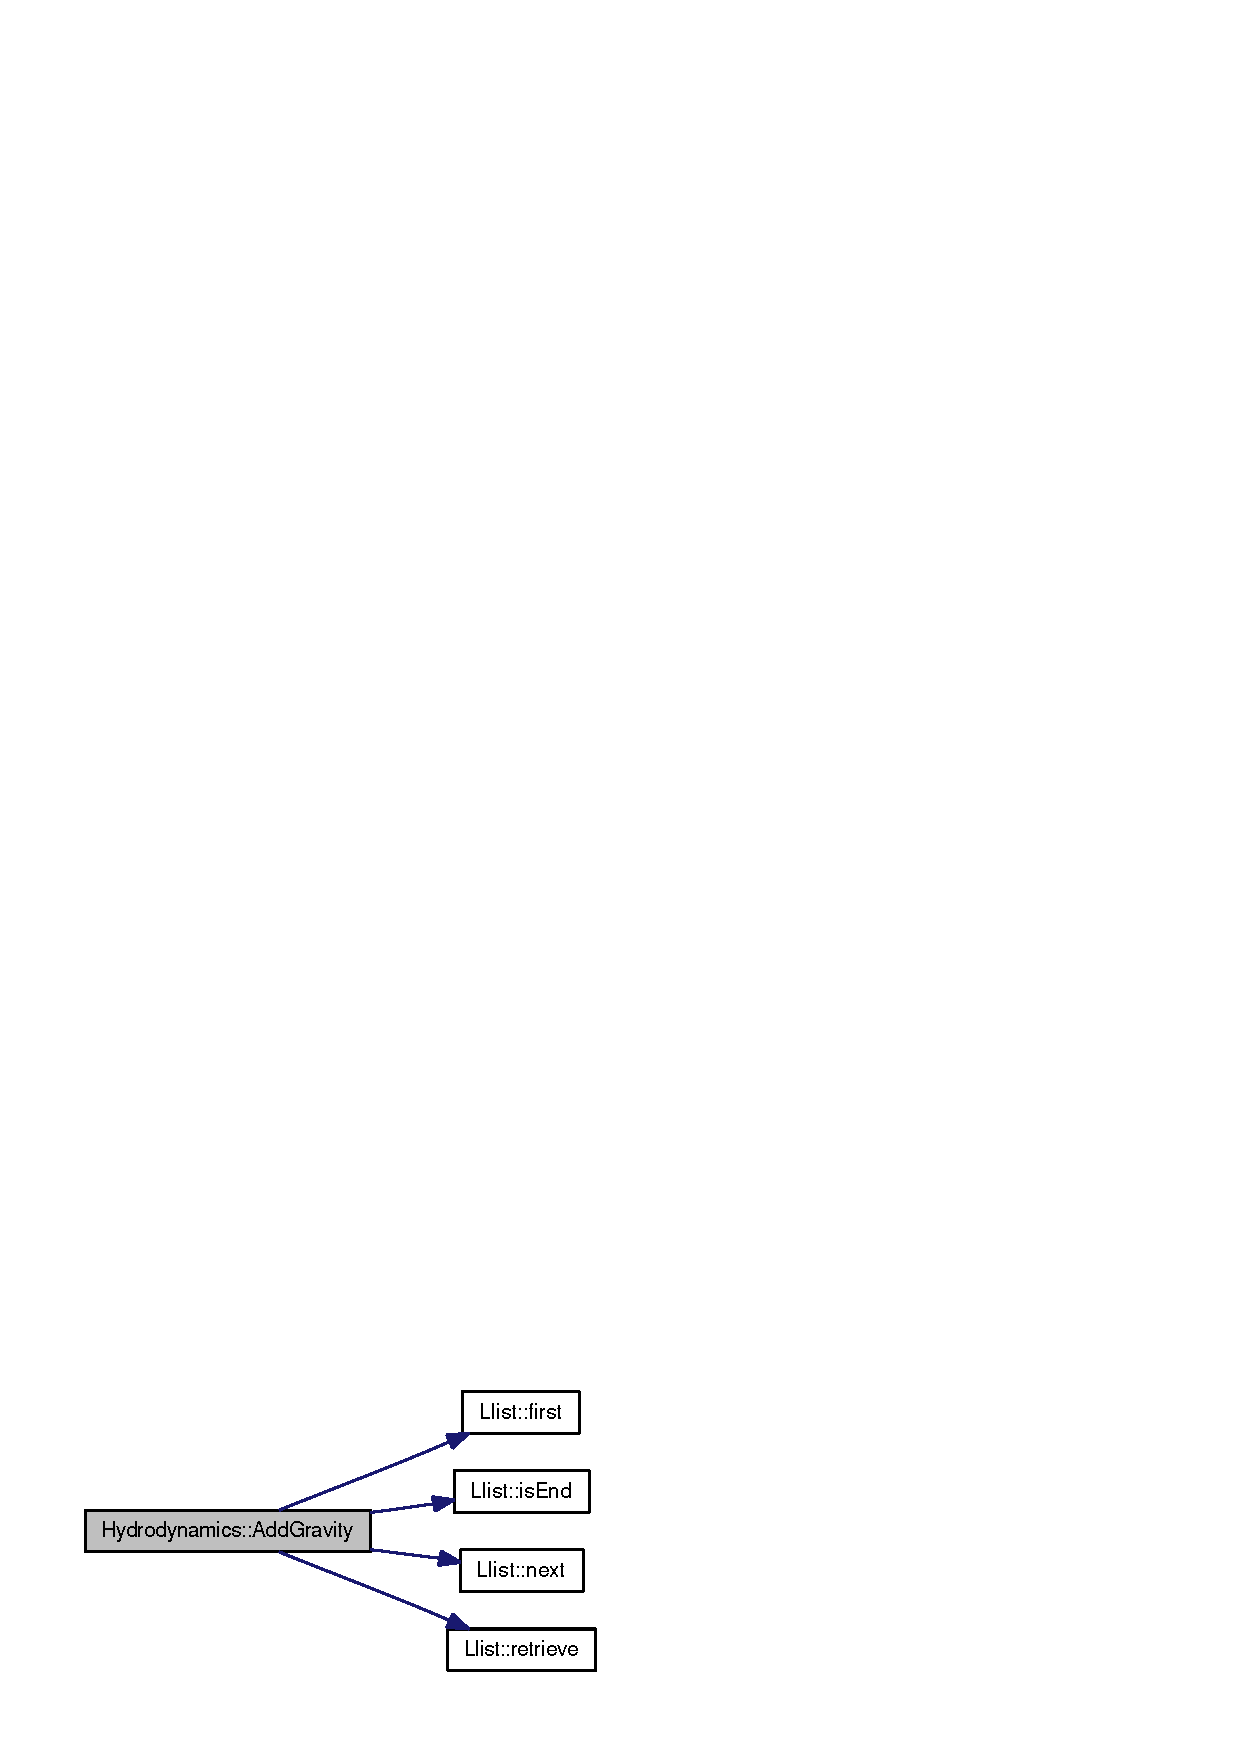
\includegraphics[width=145pt]{classHydrodynamics_abdebac769f07f2500c21689fafa2981_cgraph}
\end{center}
\end{figure}


Here is the caller graph for this function:\nopagebreak
\begin{figure}[H]
\begin{center}
\leavevmode
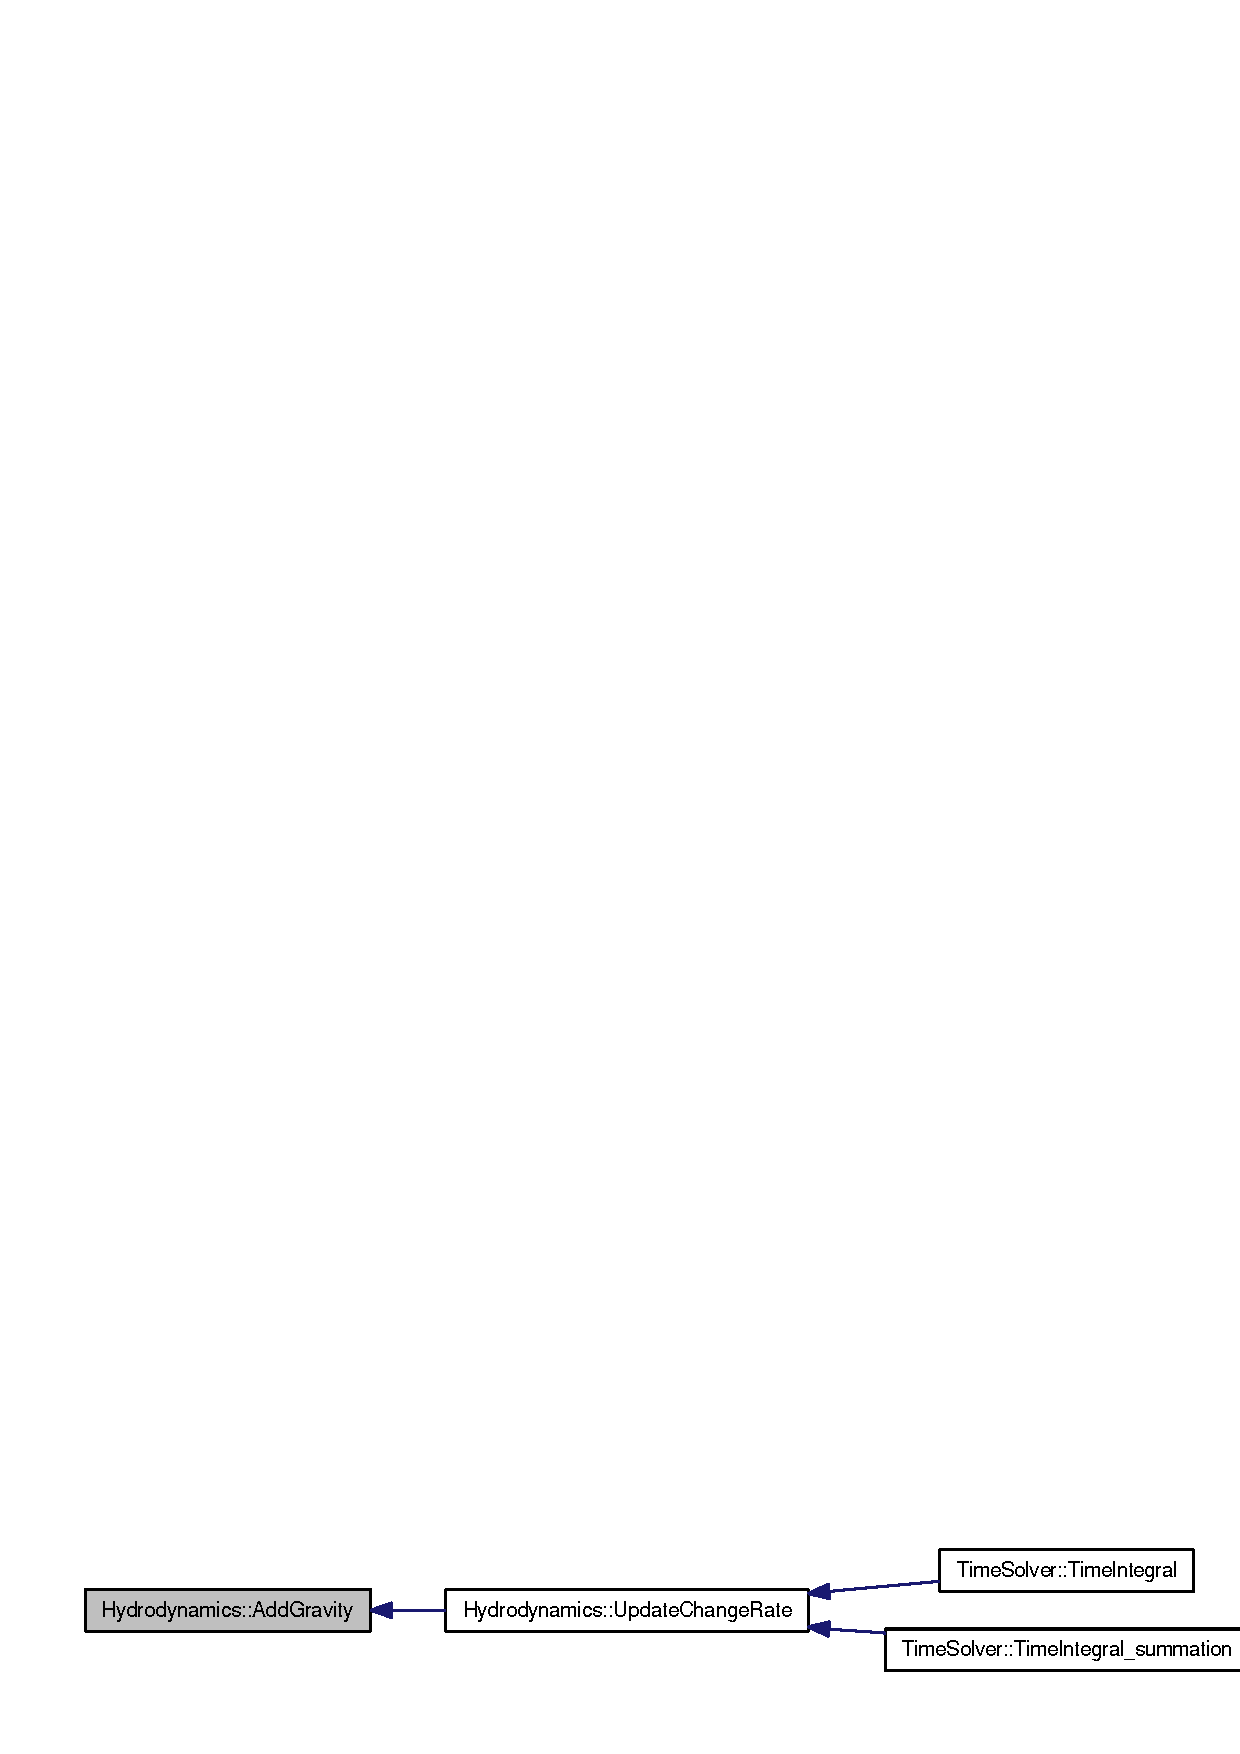
\includegraphics[width=339pt]{classHydrodynamics_abdebac769f07f2500c21689fafa2981_icgraph}
\end{center}
\end{figure}
\hypertarget{classHydrodynamics_41e1527e65d6f93d81c30467871021f5}{
\index{Hydrodynamics@{Hydrodynamics}!BuildPair@{BuildPair}}
\index{BuildPair@{BuildPair}!Hydrodynamics@{Hydrodynamics}}
\subsubsection[{BuildPair}]{\setlength{\rightskip}{0pt plus 5cm}void Hydrodynamics::BuildPair ({\bf ParticleManager} \& {\em particles}, \/  {\bf QuinticSpline} \& {\em weight\_\-function})}}
\label{classHydrodynamics_41e1527e65d6f93d81c30467871021f5}


build new pairs 



\begin{itemize}
\item obtain the interaction pairs by just calling the particles BuildInteraction method \end{itemize}


Here is the call graph for this function:\nopagebreak
\begin{figure}[H]
\begin{center}
\leavevmode
\includegraphics[width=340pt]{classHydrodynamics_41e1527e65d6f93d81c30467871021f5_cgraph}
\end{center}
\end{figure}


Here is the caller graph for this function:\nopagebreak
\begin{figure}[H]
\begin{center}
\leavevmode
\includegraphics[width=230pt]{classHydrodynamics_41e1527e65d6f93d81c30467871021f5_icgraph}
\end{center}
\end{figure}
\hypertarget{classHydrodynamics_928a3fb7752d458026ed06dca1fbf137}{
\index{Hydrodynamics@{Hydrodynamics}!Corrector@{Corrector}}
\index{Corrector@{Corrector}!Hydrodynamics@{Hydrodynamics}}
\subsubsection[{Corrector}]{\setlength{\rightskip}{0pt plus 5cm}void Hydrodynamics::Corrector (double {\em dt})}}
\label{classHydrodynamics_928a3fb7752d458026ed06dca1fbf137}


corrector method, density evaluated directly:{\bf  corrector advances p, rho, U} 



\begin{itemize}
\item iterate the real partilce list\end{itemize}


\begin{itemize}
\item for each particle: correction based on values on n step and change rate at n+1/2 \end{itemize}


Here is the call graph for this function:\nopagebreak
\begin{figure}[H]
\begin{center}
\leavevmode
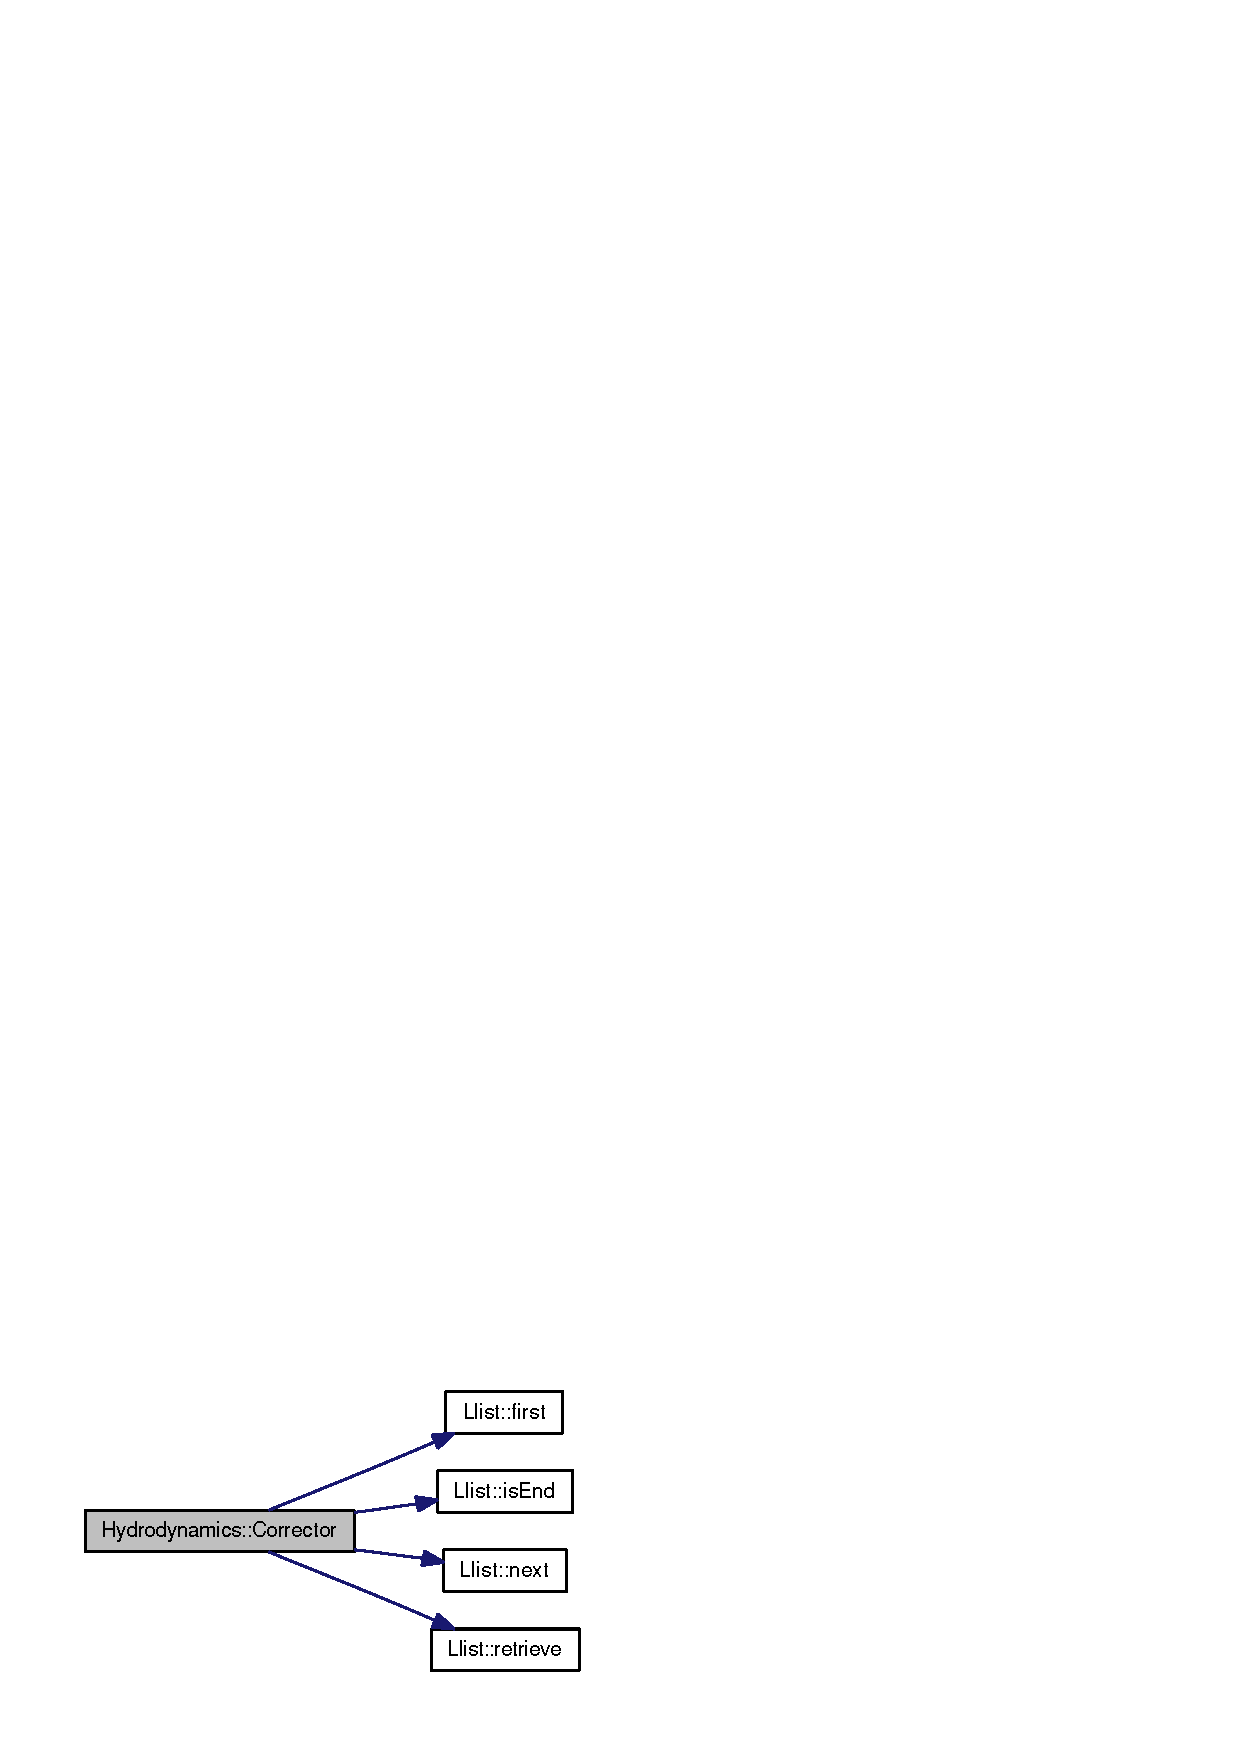
\includegraphics[width=141pt]{classHydrodynamics_928a3fb7752d458026ed06dca1fbf137_cgraph}
\end{center}
\end{figure}


Here is the caller graph for this function:\nopagebreak
\begin{figure}[H]
\begin{center}
\leavevmode
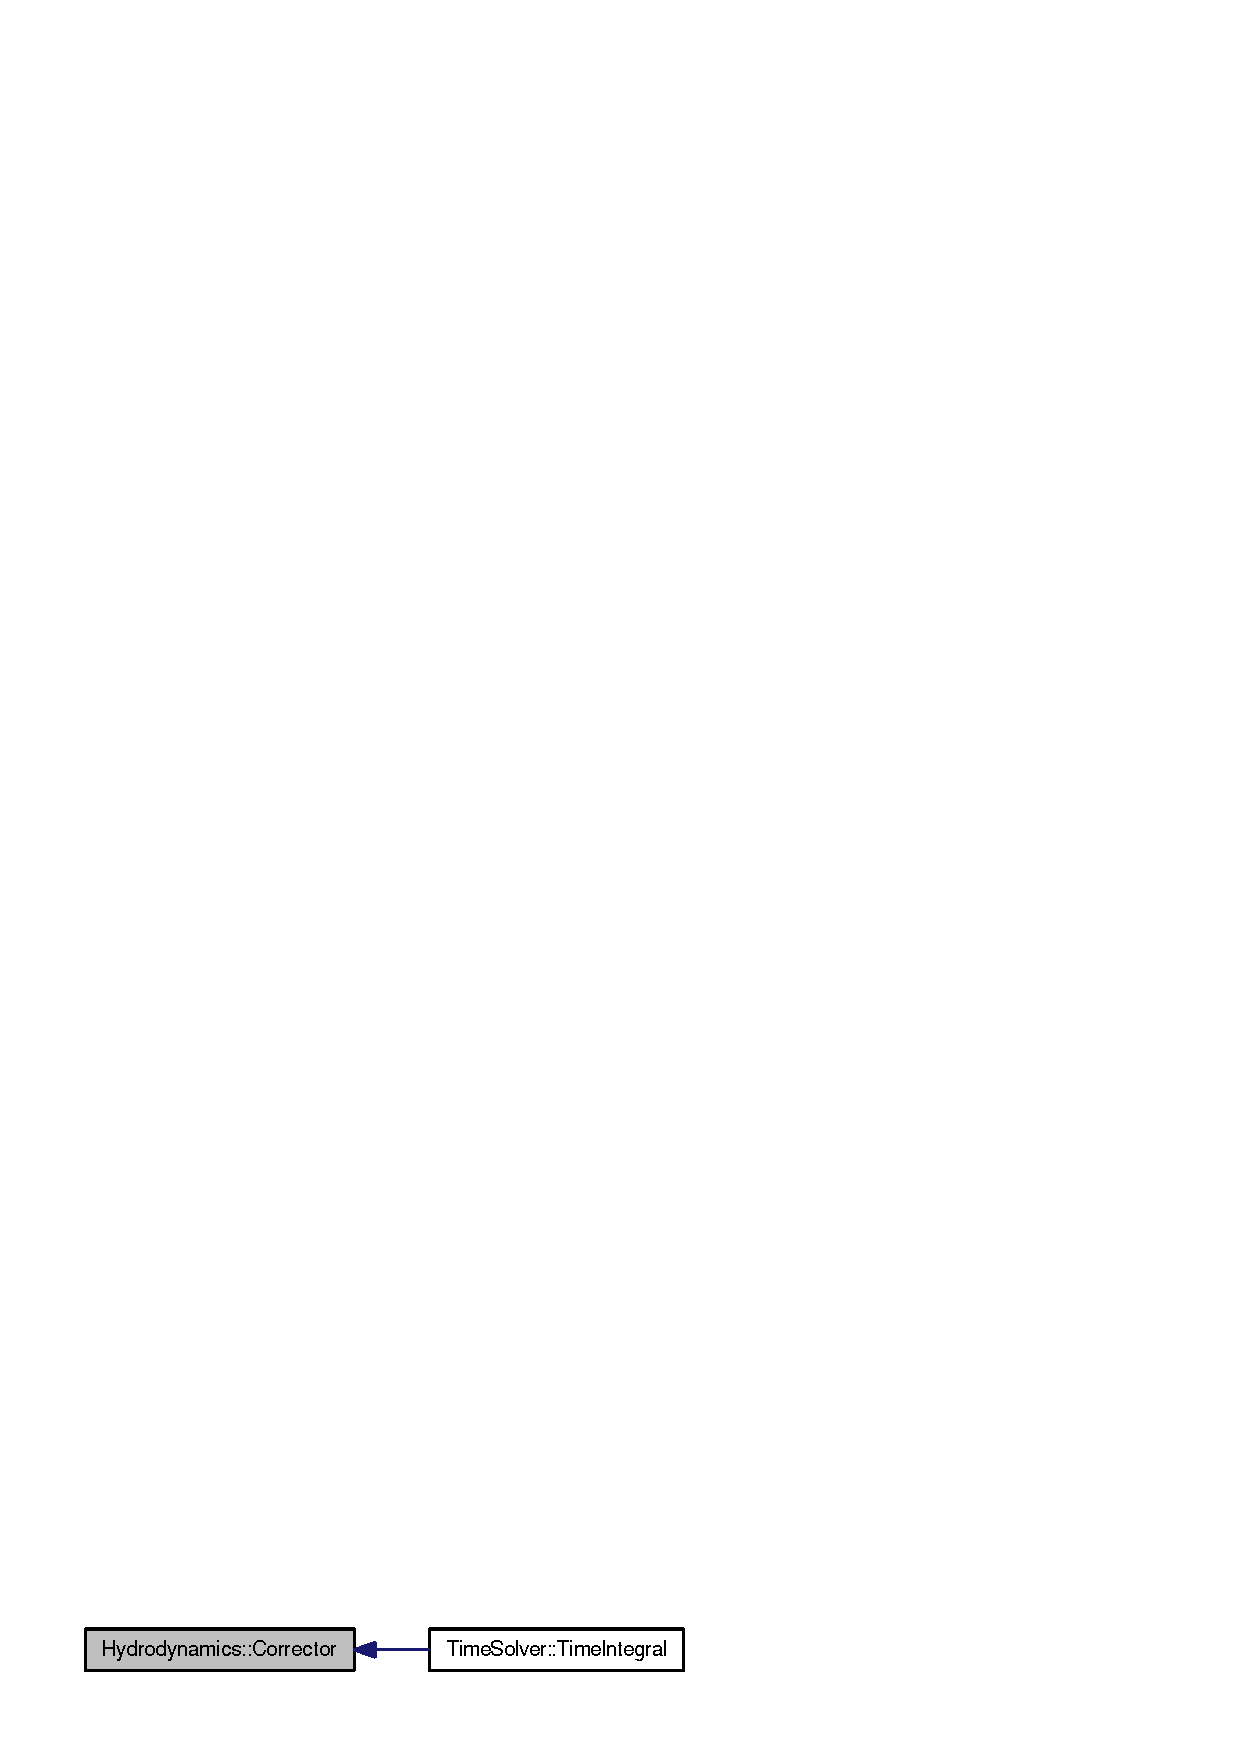
\includegraphics[width=166pt]{classHydrodynamics_928a3fb7752d458026ed06dca1fbf137_icgraph}
\end{center}
\end{figure}
\hypertarget{classHydrodynamics_6a62dad5b8c33b504481a8e4e5b023cb}{
\index{Hydrodynamics@{Hydrodynamics}!Corrector\_\-summation@{Corrector\_\-summation}}
\index{Corrector\_\-summation@{Corrector\_\-summation}!Hydrodynamics@{Hydrodynamics}}
\subsubsection[{Corrector\_\-summation}]{\setlength{\rightskip}{0pt plus 5cm}void Hydrodynamics::Corrector\_\-summation (double {\em dt})}}
\label{classHydrodynamics_6a62dad5b8c33b504481a8e4e5b023cb}


for corrector method, density evaluated with summation (that means: no density update within this method) 



\begin{itemize}
\item iterate the real partilce list\end{itemize}


\begin{itemize}
\item for each particle: correction (advances R,U) based on values on n step and change rate at n+1/2 \end{itemize}


Here is the call graph for this function:\nopagebreak
\begin{figure}[H]
\begin{center}
\leavevmode
\includegraphics[width=168pt]{classHydrodynamics_6a62dad5b8c33b504481a8e4e5b023cb_cgraph}
\end{center}
\end{figure}


Here is the caller graph for this function:\nopagebreak
\begin{figure}[H]
\begin{center}
\leavevmode
\includegraphics[width=257pt]{classHydrodynamics_6a62dad5b8c33b504481a8e4e5b023cb_icgraph}
\end{center}
\end{figure}
\hypertarget{classHydrodynamics_316a6079bf22102d9b911e2632cd2680}{
\index{Hydrodynamics@{Hydrodynamics}!Predictor@{Predictor}}
\index{Predictor@{Predictor}!Hydrodynamics@{Hydrodynamics}}
\subsubsection[{Predictor}]{\setlength{\rightskip}{0pt plus 5cm}void Hydrodynamics::Predictor (double {\em dt})}}
\label{classHydrodynamics_316a6079bf22102d9b911e2632cd2680}


predictor method, density evaluated directly 



\begin{itemize}
\item iterate the real partilce list

\begin{itemize}
\item save values at step n

\item predict values at step n+1

\item calculate the middle values at step n+1/2\end{itemize}
\end{itemize}


Here is the call graph for this function:\nopagebreak
\begin{figure}[H]
\begin{center}
\leavevmode
\includegraphics[width=141pt]{classHydrodynamics_316a6079bf22102d9b911e2632cd2680_cgraph}
\end{center}
\end{figure}


Here is the caller graph for this function:\nopagebreak
\begin{figure}[H]
\begin{center}
\leavevmode
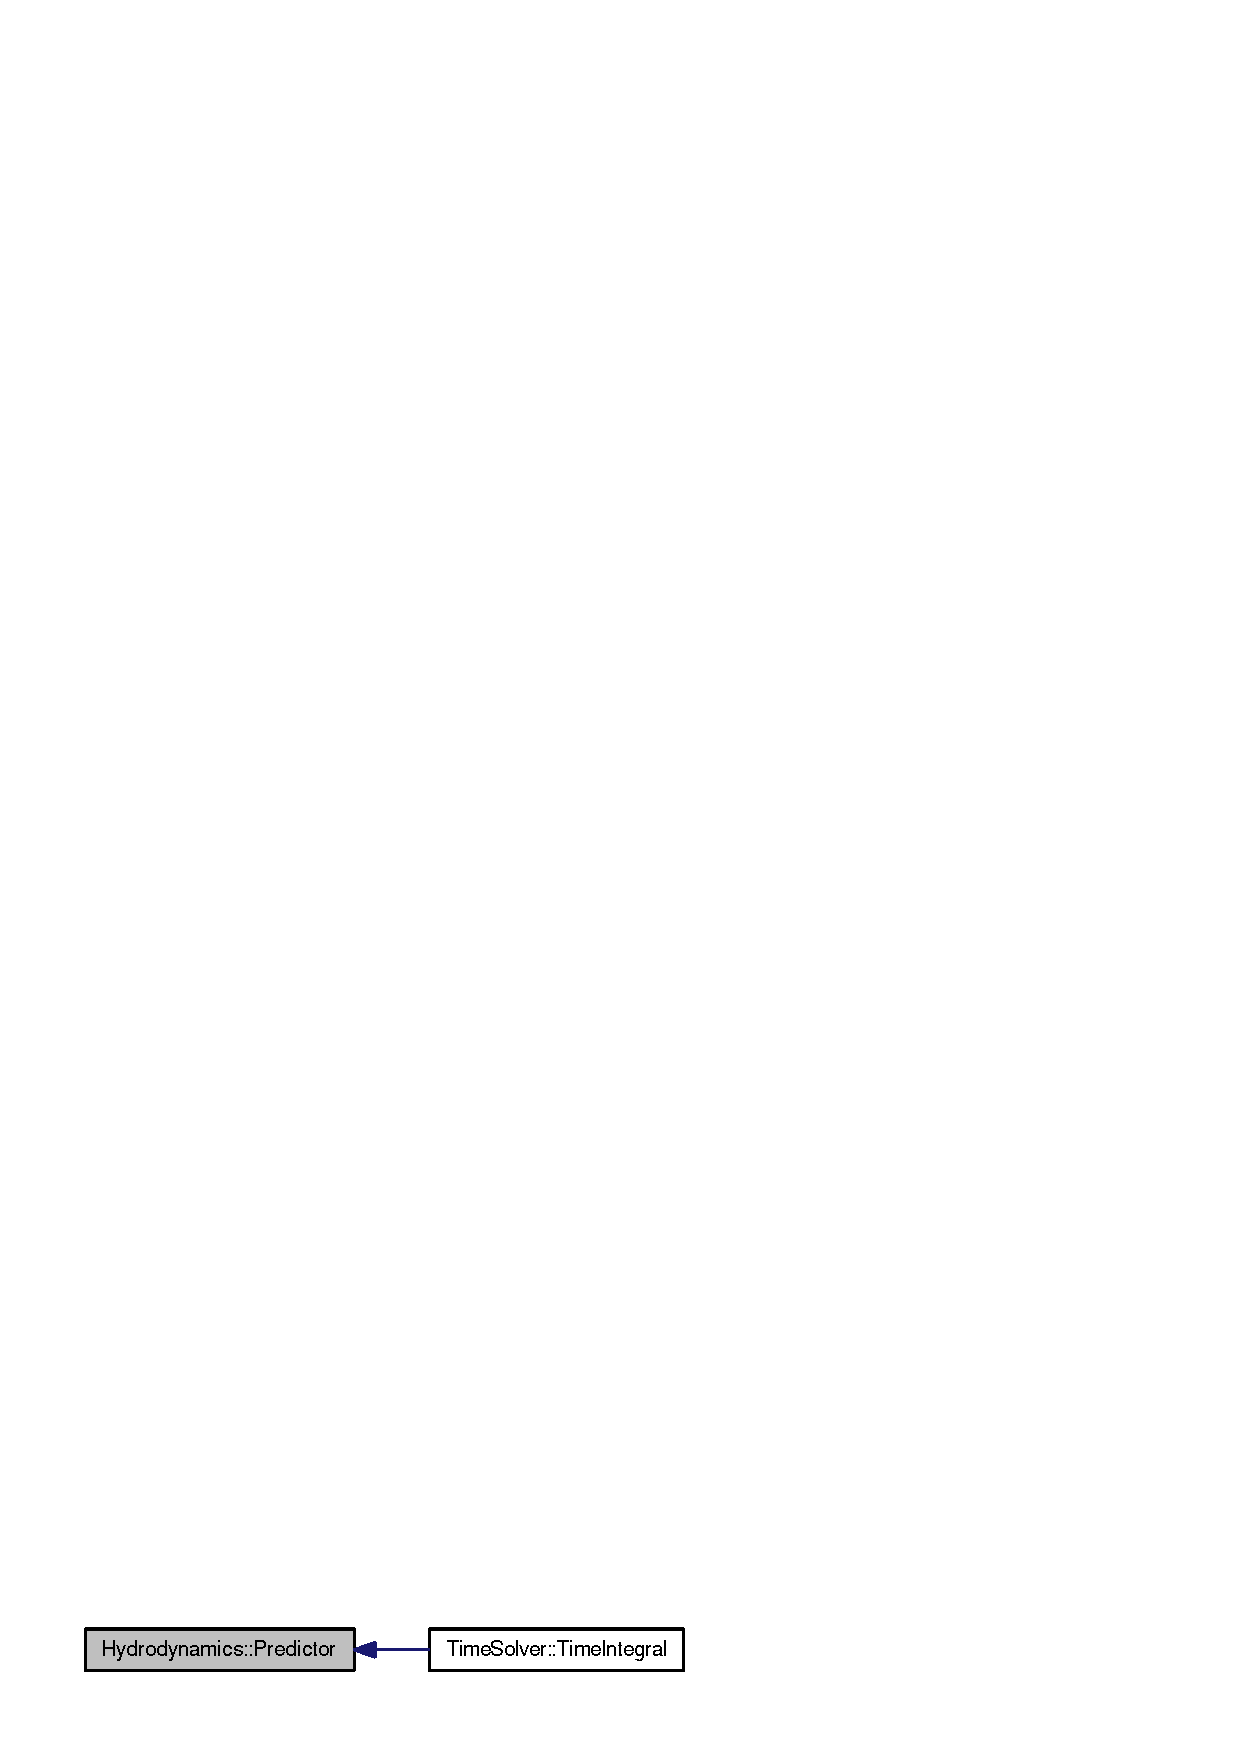
\includegraphics[width=166pt]{classHydrodynamics_316a6079bf22102d9b911e2632cd2680_icgraph}
\end{center}
\end{figure}
\hypertarget{classHydrodynamics_911fe25b94fec398fad1f2def036d755}{
\index{Hydrodynamics@{Hydrodynamics}!Predictor\_\-summation@{Predictor\_\-summation}}
\index{Predictor\_\-summation@{Predictor\_\-summation}!Hydrodynamics@{Hydrodynamics}}
\subsubsection[{Predictor\_\-summation}]{\setlength{\rightskip}{0pt plus 5cm}void Hydrodynamics::Predictor\_\-summation (double {\em dt})}}
\label{classHydrodynamics_911fe25b94fec398fad1f2def036d755}


for predictor method, density evaluated with summation (that means: no density update within this method) 



\begin{itemize}
\item iterate the real partilce list

\begin{itemize}
\item save values (R,U) at step n in intermediate variables .\_\-I

\item predict values at step n+1

\item calculate the middle values at step n+1/2 and save them in \hyperlink{classParticle}{Particle} objects prtl\end{itemize}
\end{itemize}


Here is the call graph for this function:\nopagebreak
\begin{figure}[H]
\begin{center}
\leavevmode
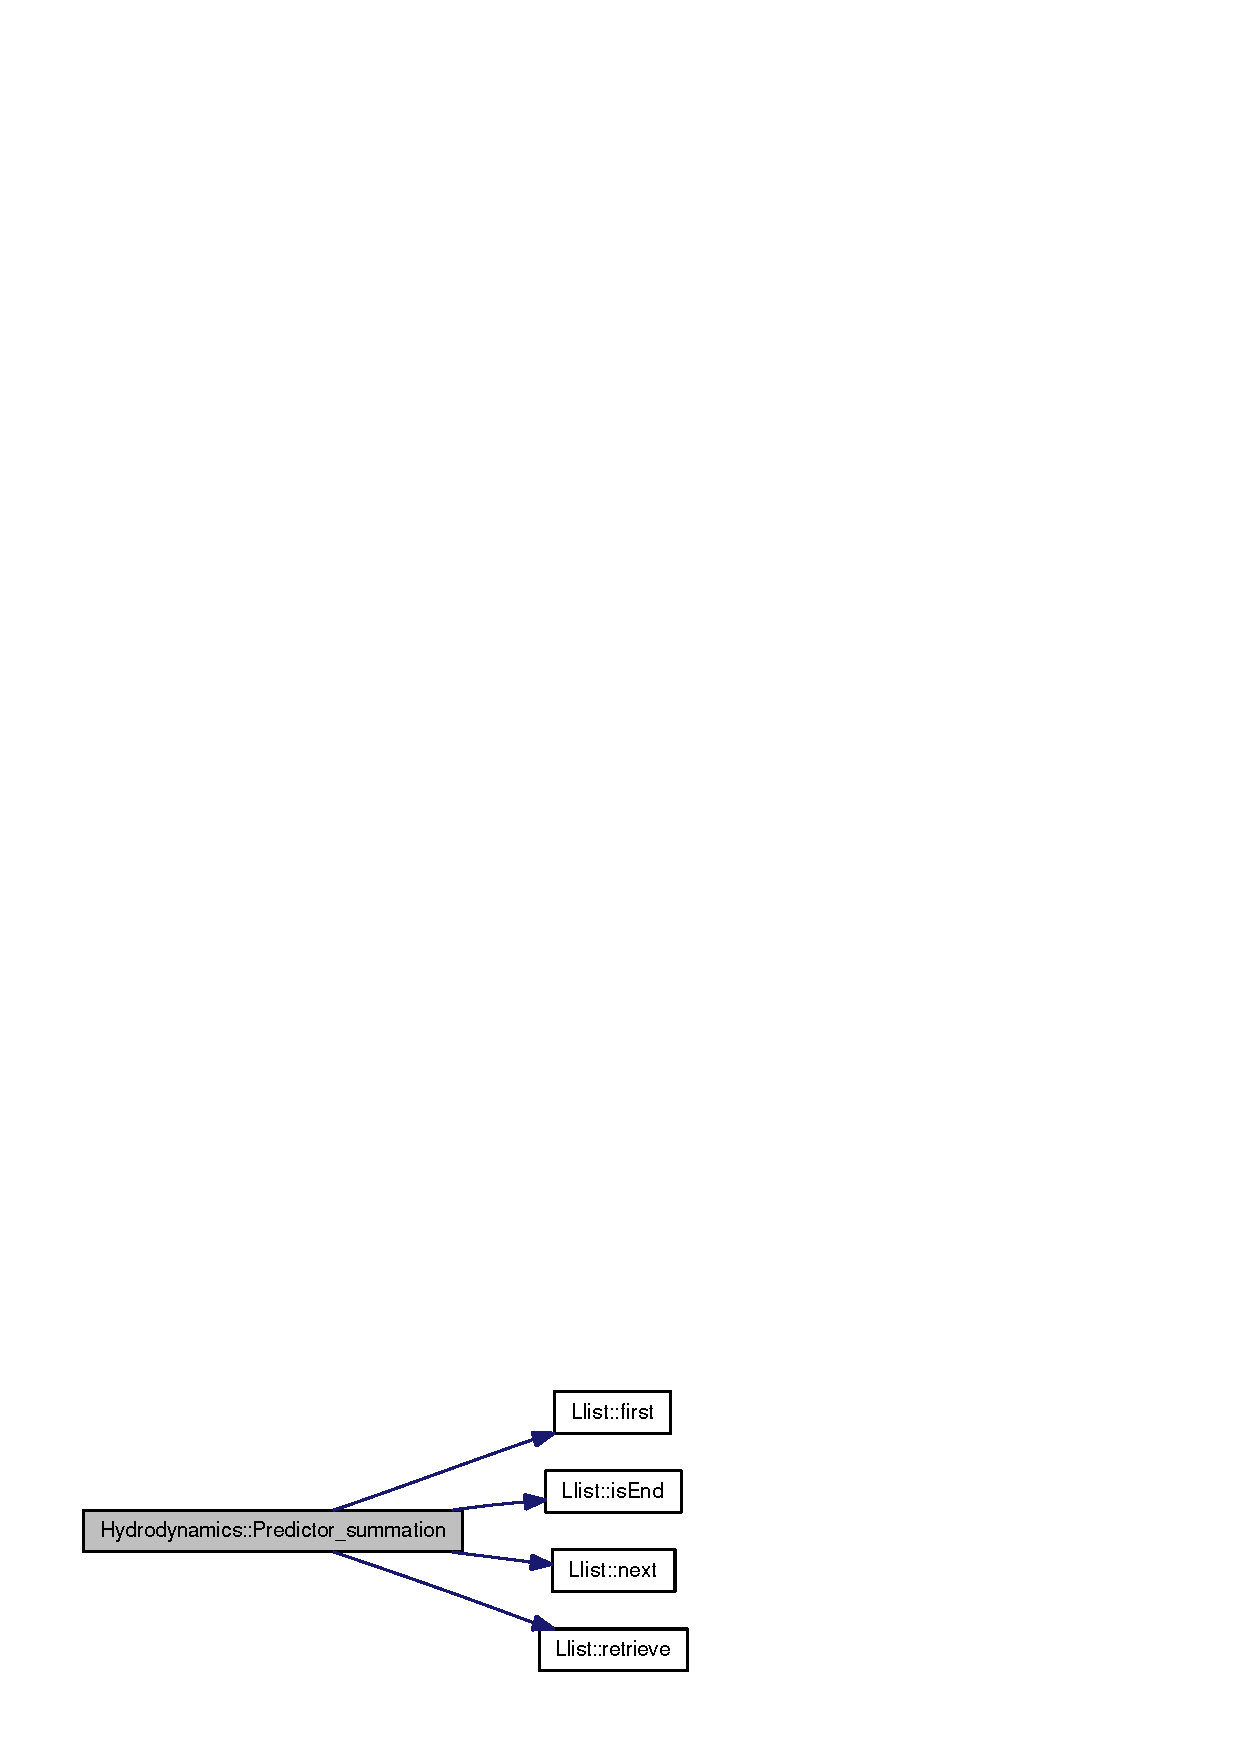
\includegraphics[width=167pt]{classHydrodynamics_911fe25b94fec398fad1f2def036d755_cgraph}
\end{center}
\end{figure}


Here is the caller graph for this function:\nopagebreak
\begin{figure}[H]
\begin{center}
\leavevmode
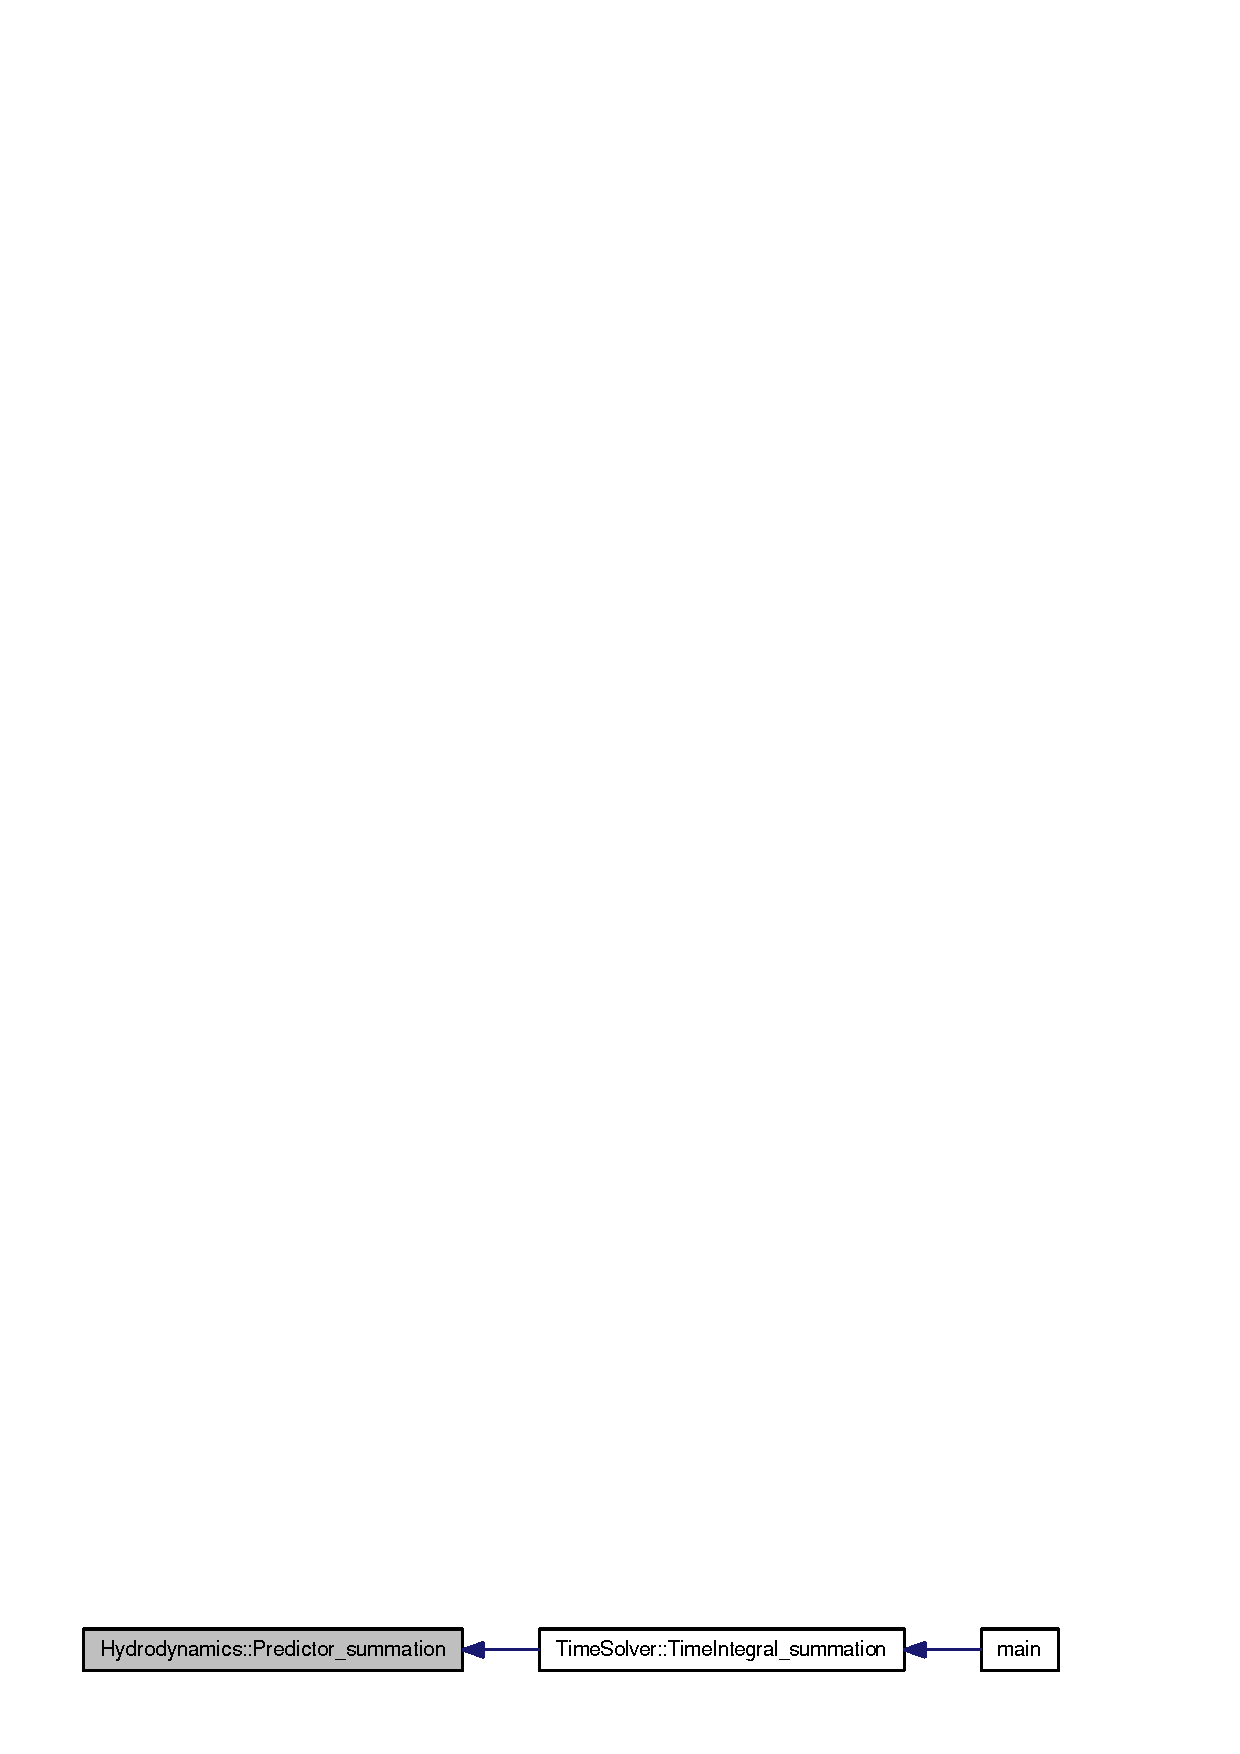
\includegraphics[width=256pt]{classHydrodynamics_911fe25b94fec398fad1f2def036d755_icgraph}
\end{center}
\end{figure}
\hypertarget{classHydrodynamics_8f826d2003ca7a4782b028b761a26421}{
\index{Hydrodynamics@{Hydrodynamics}!RandomEffects@{RandomEffects}}
\index{RandomEffects@{RandomEffects}!Hydrodynamics@{Hydrodynamics}}
\subsubsection[{RandomEffects}]{\setlength{\rightskip}{0pt plus 5cm}void Hydrodynamics::RandomEffects ()}}
\label{classHydrodynamics_8f826d2003ca7a4782b028b761a26421}


including random effects (DPD simulation) 



\begin{itemize}
\item iterate the real partilce list\end{itemize}


\begin{itemize}
\item for each particle: add random velocity \_\-dU \end{itemize}


Here is the call graph for this function:\nopagebreak
\begin{figure}[H]
\begin{center}
\leavevmode
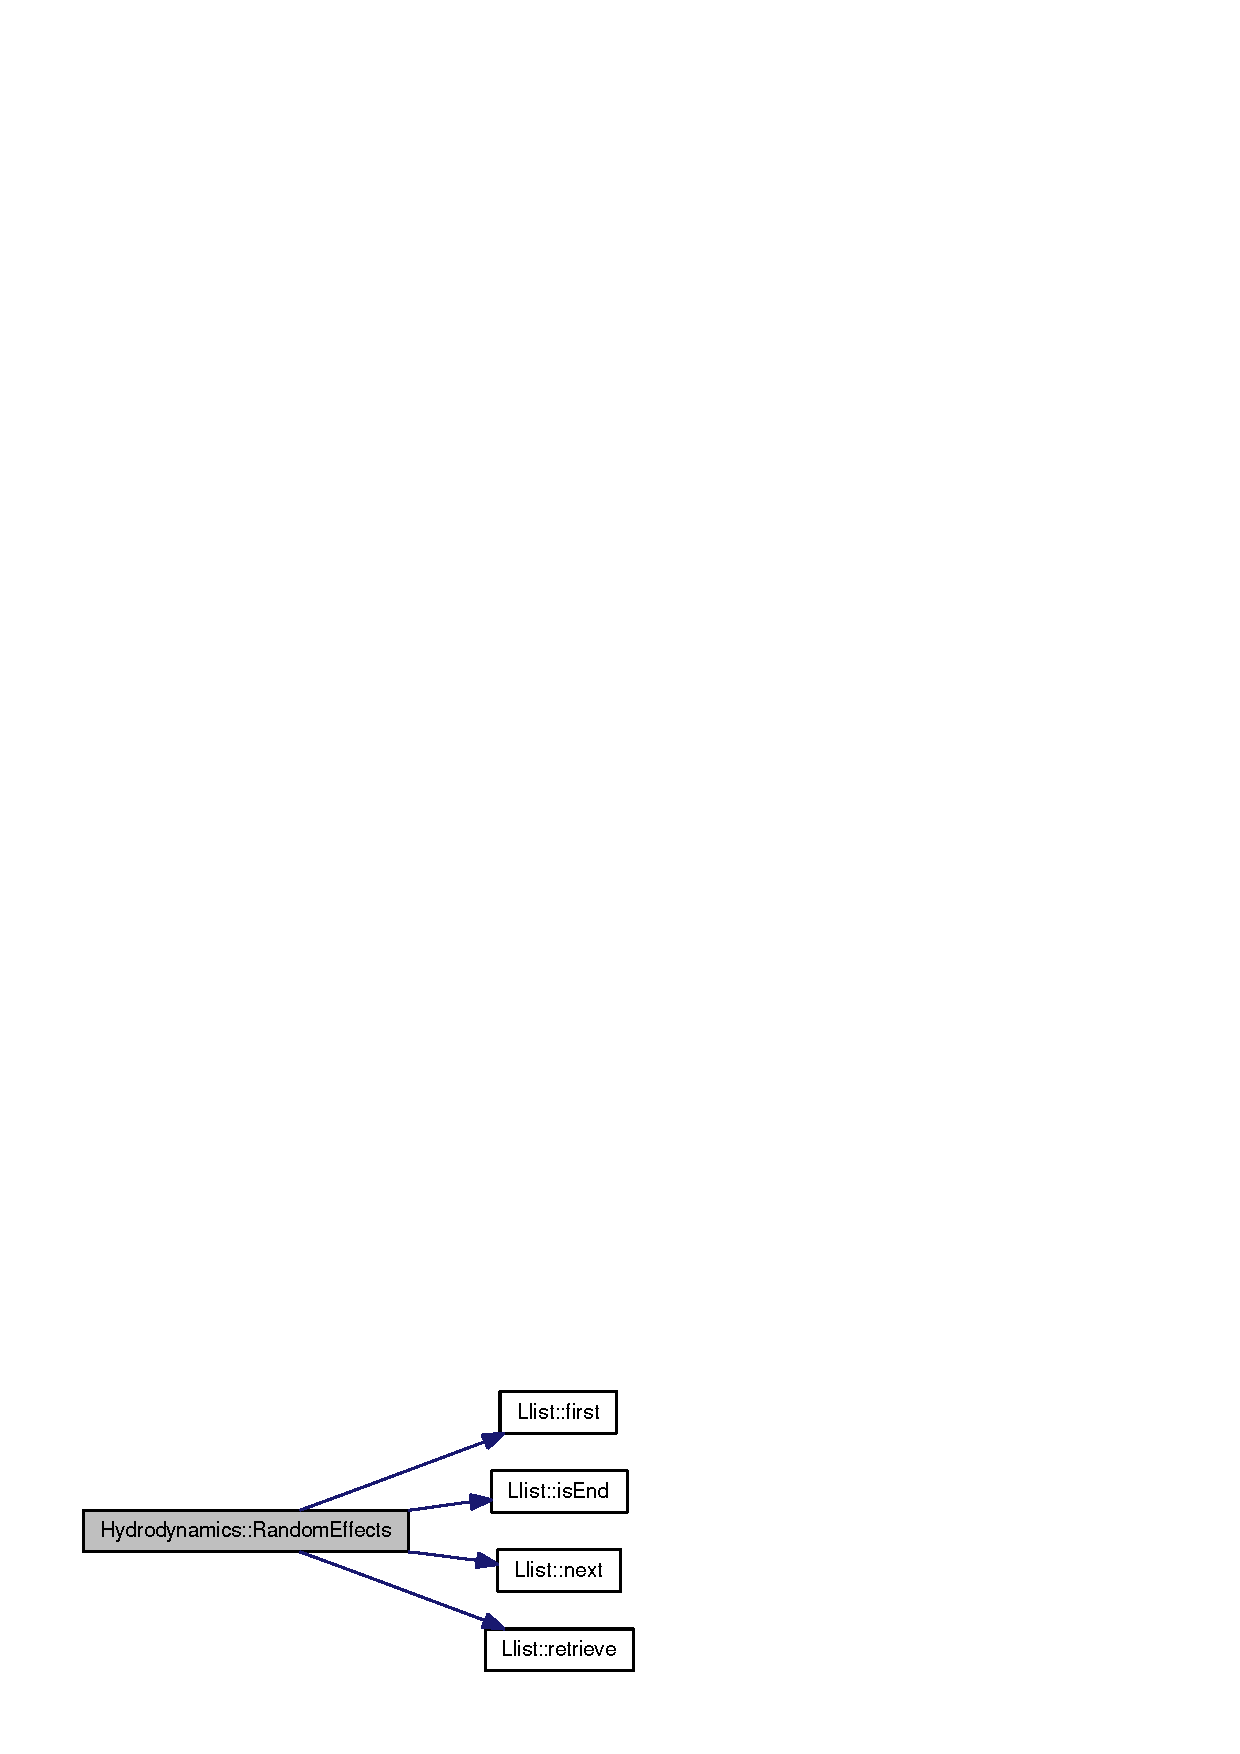
\includegraphics[width=154pt]{classHydrodynamics_8f826d2003ca7a4782b028b761a26421_cgraph}
\end{center}
\end{figure}


Here is the caller graph for this function:\nopagebreak
\begin{figure}[H]
\begin{center}
\leavevmode
\includegraphics[width=179pt]{classHydrodynamics_8f826d2003ca7a4782b028b761a26421_icgraph}
\end{center}
\end{figure}
\hypertarget{classHydrodynamics_e6983cf4d86bf7b33b88c8f089caf3a8}{
\index{Hydrodynamics@{Hydrodynamics}!SurfaceTensionCoefficient@{SurfaceTensionCoefficient}}
\index{SurfaceTensionCoefficient@{SurfaceTensionCoefficient}!Hydrodynamics@{Hydrodynamics}}
\subsubsection[{SurfaceTensionCoefficient}]{\setlength{\rightskip}{0pt plus 5cm}double Hydrodynamics::SurfaceTensionCoefficient ()}}
\label{classHydrodynamics_e6983cf4d86bf7b33b88c8f089caf3a8}


calculate surface tension coefficient 



\begin{itemize}
\item iterate particles on the real particle list\end{itemize}


\begin{itemize}
\item calculate phase surface stress for all particles \end{itemize}


Here is the call graph for this function:\nopagebreak
\begin{figure}[H]
\begin{center}
\leavevmode
\includegraphics[width=177pt]{classHydrodynamics_e6983cf4d86bf7b33b88c8f089caf3a8_cgraph}
\end{center}
\end{figure}
\hypertarget{classHydrodynamics_f744ee07f3f3b511d0db18949160c20a}{
\index{Hydrodynamics@{Hydrodynamics}!UpdateChangeRate@{UpdateChangeRate}}
\index{UpdateChangeRate@{UpdateChangeRate}!Hydrodynamics@{Hydrodynamics}}
\subsubsection[{UpdateChangeRate}]{\setlength{\rightskip}{0pt plus 5cm}void Hydrodynamics::UpdateChangeRate ()}}
\label{classHydrodynamics_f744ee07f3f3b511d0db18949160c20a}


calculate interaction without updating interaction list 



\begin{itemize}
\item initiate the change rate of each real particle by calling \hyperlink{classHydrodynamics_67e2d72d69156a086d43168f5cd58bf7}{ZeroChangeRate()}\end{itemize}


\begin{itemize}
\item iterate the interaction list\end{itemize}


\begin{itemize}
\item calculate for each pair the pair forces or change rate\end{itemize}


\begin{itemize}
\item include the gravity effects \end{itemize}


Here is the call graph for this function:\nopagebreak
\begin{figure}[H]
\begin{center}
\leavevmode
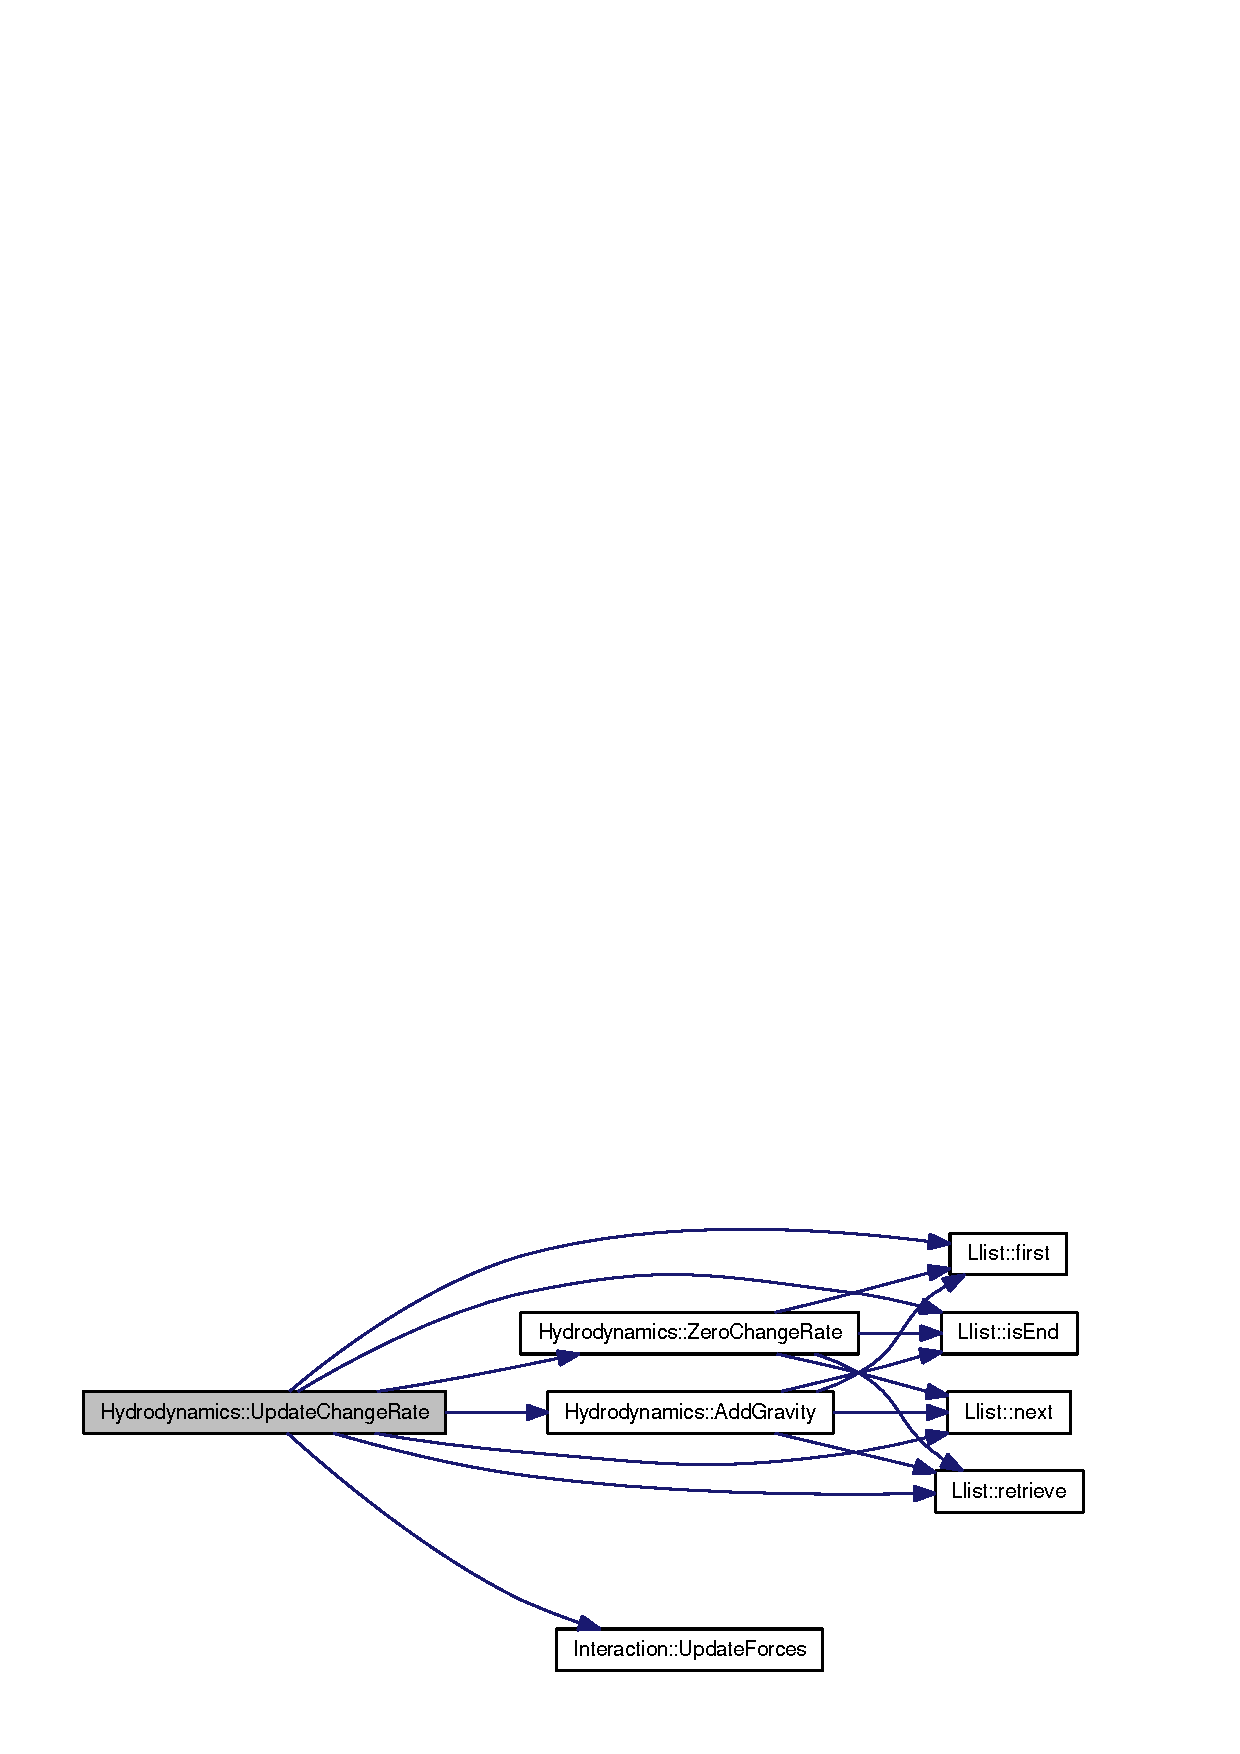
\includegraphics[width=262pt]{classHydrodynamics_f744ee07f3f3b511d0db18949160c20a_cgraph}
\end{center}
\end{figure}
\hypertarget{classHydrodynamics_22df8569d81c4c363029efac143ddb26}{
\index{Hydrodynamics@{Hydrodynamics}!UpdateChangeRate@{UpdateChangeRate}}
\index{UpdateChangeRate@{UpdateChangeRate}!Hydrodynamics@{Hydrodynamics}}
\subsubsection[{UpdateChangeRate}]{\setlength{\rightskip}{0pt plus 5cm}void Hydrodynamics::UpdateChangeRate ({\bf ParticleManager} \& {\em particles}, \/  {\bf QuinticSpline} \& {\em weight\_\-function})}}
\label{classHydrodynamics_22df8569d81c4c363029efac143ddb26}


calculate interaction with updating interaction list 



\begin{itemize}
\item initiate change rate of each real particle by calling ZerpChangeRate()\end{itemize}


\begin{itemize}
\item obtain the interaction pairs\end{itemize}


\begin{itemize}
\item iterate the interaction list\end{itemize}


\begin{itemize}
\item calculate for eahc pair the pair forces or change rate\end{itemize}


\begin{itemize}
\item include the gravity effects by calling \hyperlink{classHydrodynamics_abdebac769f07f2500c21689fafa2981}{AddGravity()} \end{itemize}


Here is the call graph for this function:\nopagebreak
\begin{figure}[H]
\begin{center}
\leavevmode
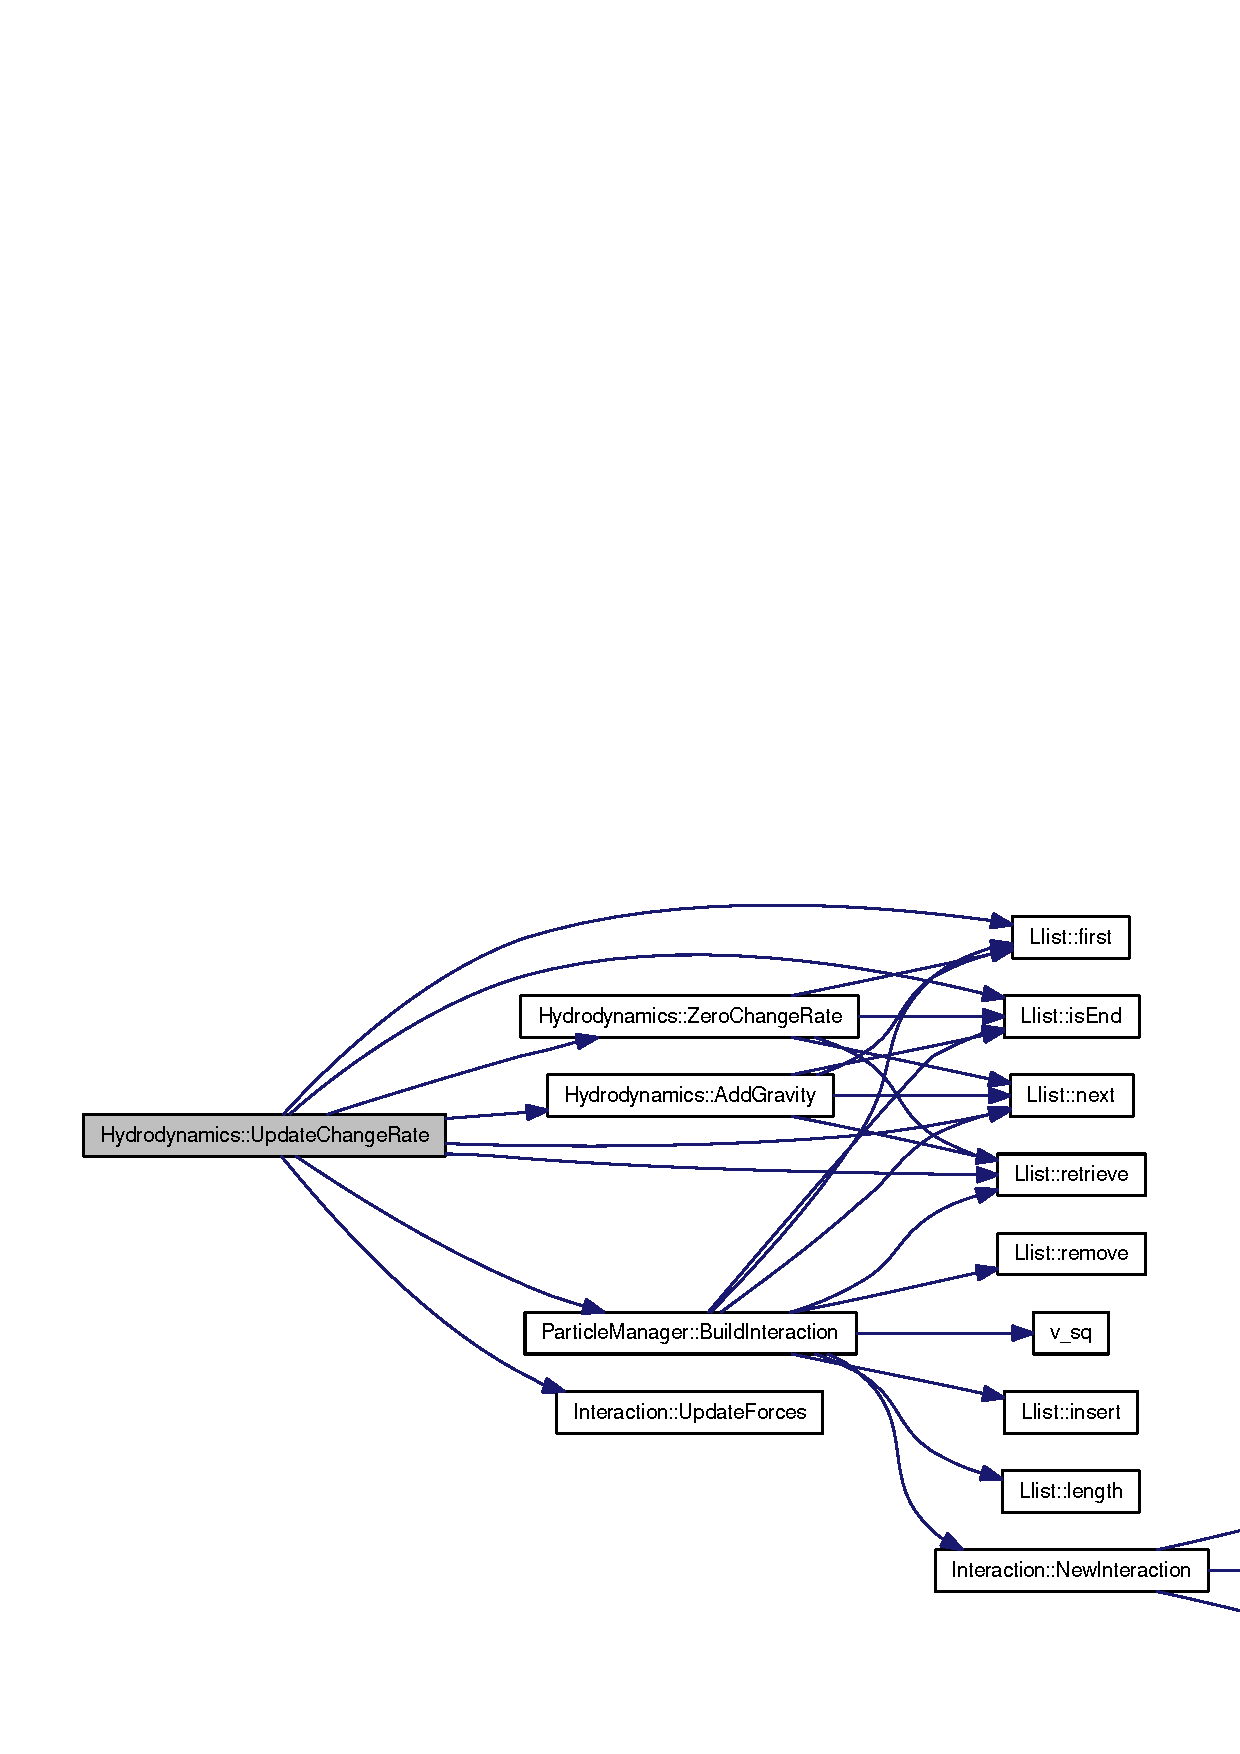
\includegraphics[width=363pt]{classHydrodynamics_22df8569d81c4c363029efac143ddb26_cgraph}
\end{center}
\end{figure}


Here is the caller graph for this function:\nopagebreak
\begin{figure}[H]
\begin{center}
\leavevmode
\includegraphics[width=252pt]{classHydrodynamics_22df8569d81c4c363029efac143ddb26_icgraph}
\end{center}
\end{figure}
\hypertarget{classHydrodynamics_b6cab35a4d7adf70657ef16b9ec4dafd}{
\index{Hydrodynamics@{Hydrodynamics}!UpdateDensity@{UpdateDensity}}
\index{UpdateDensity@{UpdateDensity}!Hydrodynamics@{Hydrodynamics}}
\subsubsection[{UpdateDensity}]{\setlength{\rightskip}{0pt plus 5cm}void Hydrodynamics::UpdateDensity ()}}
\label{classHydrodynamics_b6cab35a4d7adf70657ef16b9ec4dafd}


currently no shear rate calculated without updating interaction list 



\begin{itemize}
\item initiate zero density\end{itemize}


\begin{itemize}
\item iterate the interaction list\end{itemize}


\begin{itemize}
\item calculate for each pair the pair forces or change rate\end{itemize}


\begin{itemize}
\item calulate new pressure by calling \hyperlink{classHydrodynamics_1698dbe8ecc0e730319de5d7eca7a891}{UpdateState()} \end{itemize}


Here is the call graph for this function:\nopagebreak
\begin{figure}[H]
\begin{center}
\leavevmode
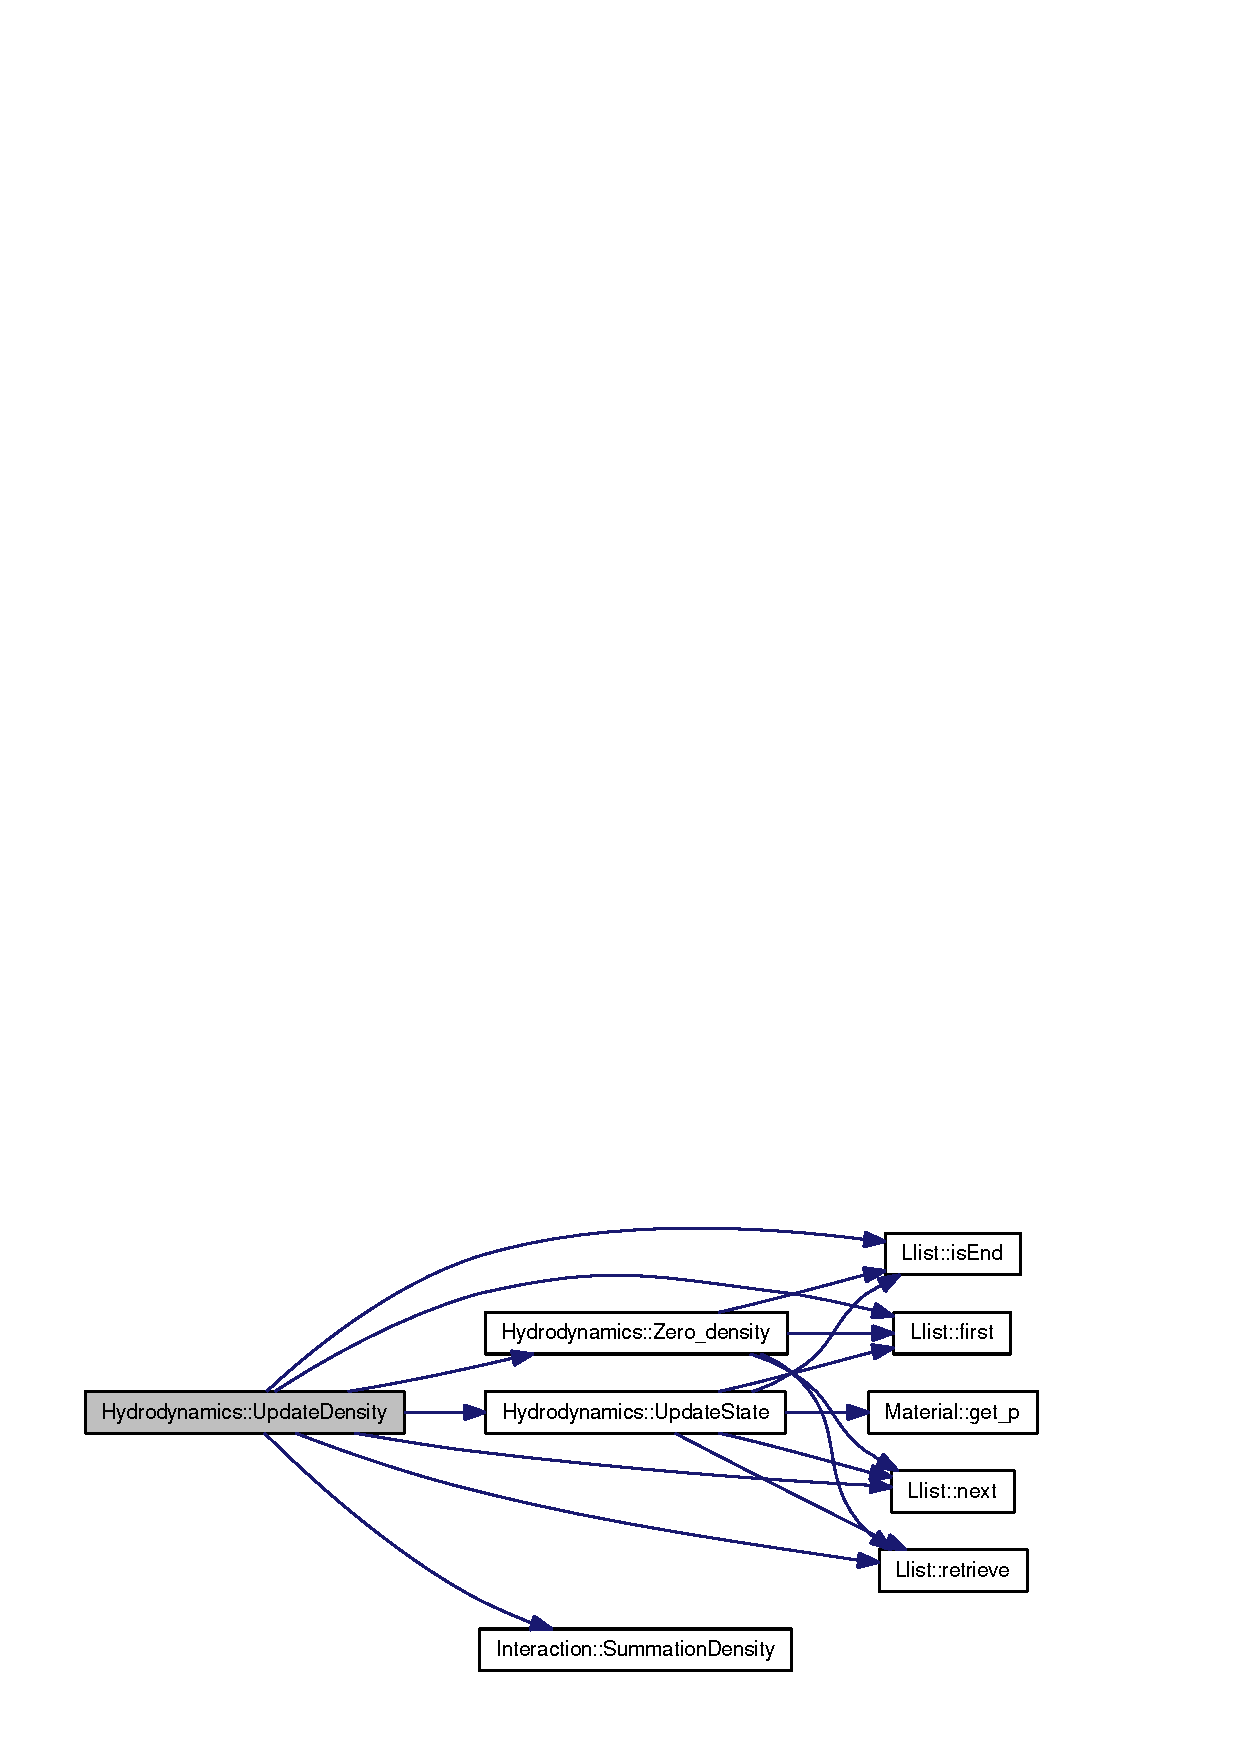
\includegraphics[width=251pt]{classHydrodynamics_b6cab35a4d7adf70657ef16b9ec4dafd_cgraph}
\end{center}
\end{figure}
\hypertarget{classHydrodynamics_1818eb1f9044ae980e92c70146e51c5b}{
\index{Hydrodynamics@{Hydrodynamics}!UpdateDensity@{UpdateDensity}}
\index{UpdateDensity@{UpdateDensity}!Hydrodynamics@{Hydrodynamics}}
\subsubsection[{UpdateDensity}]{\setlength{\rightskip}{0pt plus 5cm}void Hydrodynamics::UpdateDensity ({\bf ParticleManager} \& {\em particles}, \/  {\bf QuinticSpline} \& {\em weight\_\-function})}}
\label{classHydrodynamics_1818eb1f9044ae980e92c70146e51c5b}


summation for particles density (with updating interaction list) 



\begin{itemize}
\item obtain the interaction pairs\end{itemize}


\begin{itemize}
\item initiate by calling Zero\_\-density method\end{itemize}


\begin{itemize}
\item iterate the interaction list\end{itemize}


\begin{itemize}
\item calculate for each pair the pair forces or change rate by calling SummationDensity() method\end{itemize}


\begin{itemize}
\item calulate new pressure by calling \hyperlink{classHydrodynamics_1698dbe8ecc0e730319de5d7eca7a891}{UpdateState()} Method \end{itemize}


Here is the call graph for this function:\nopagebreak
\begin{figure}[H]
\begin{center}
\leavevmode
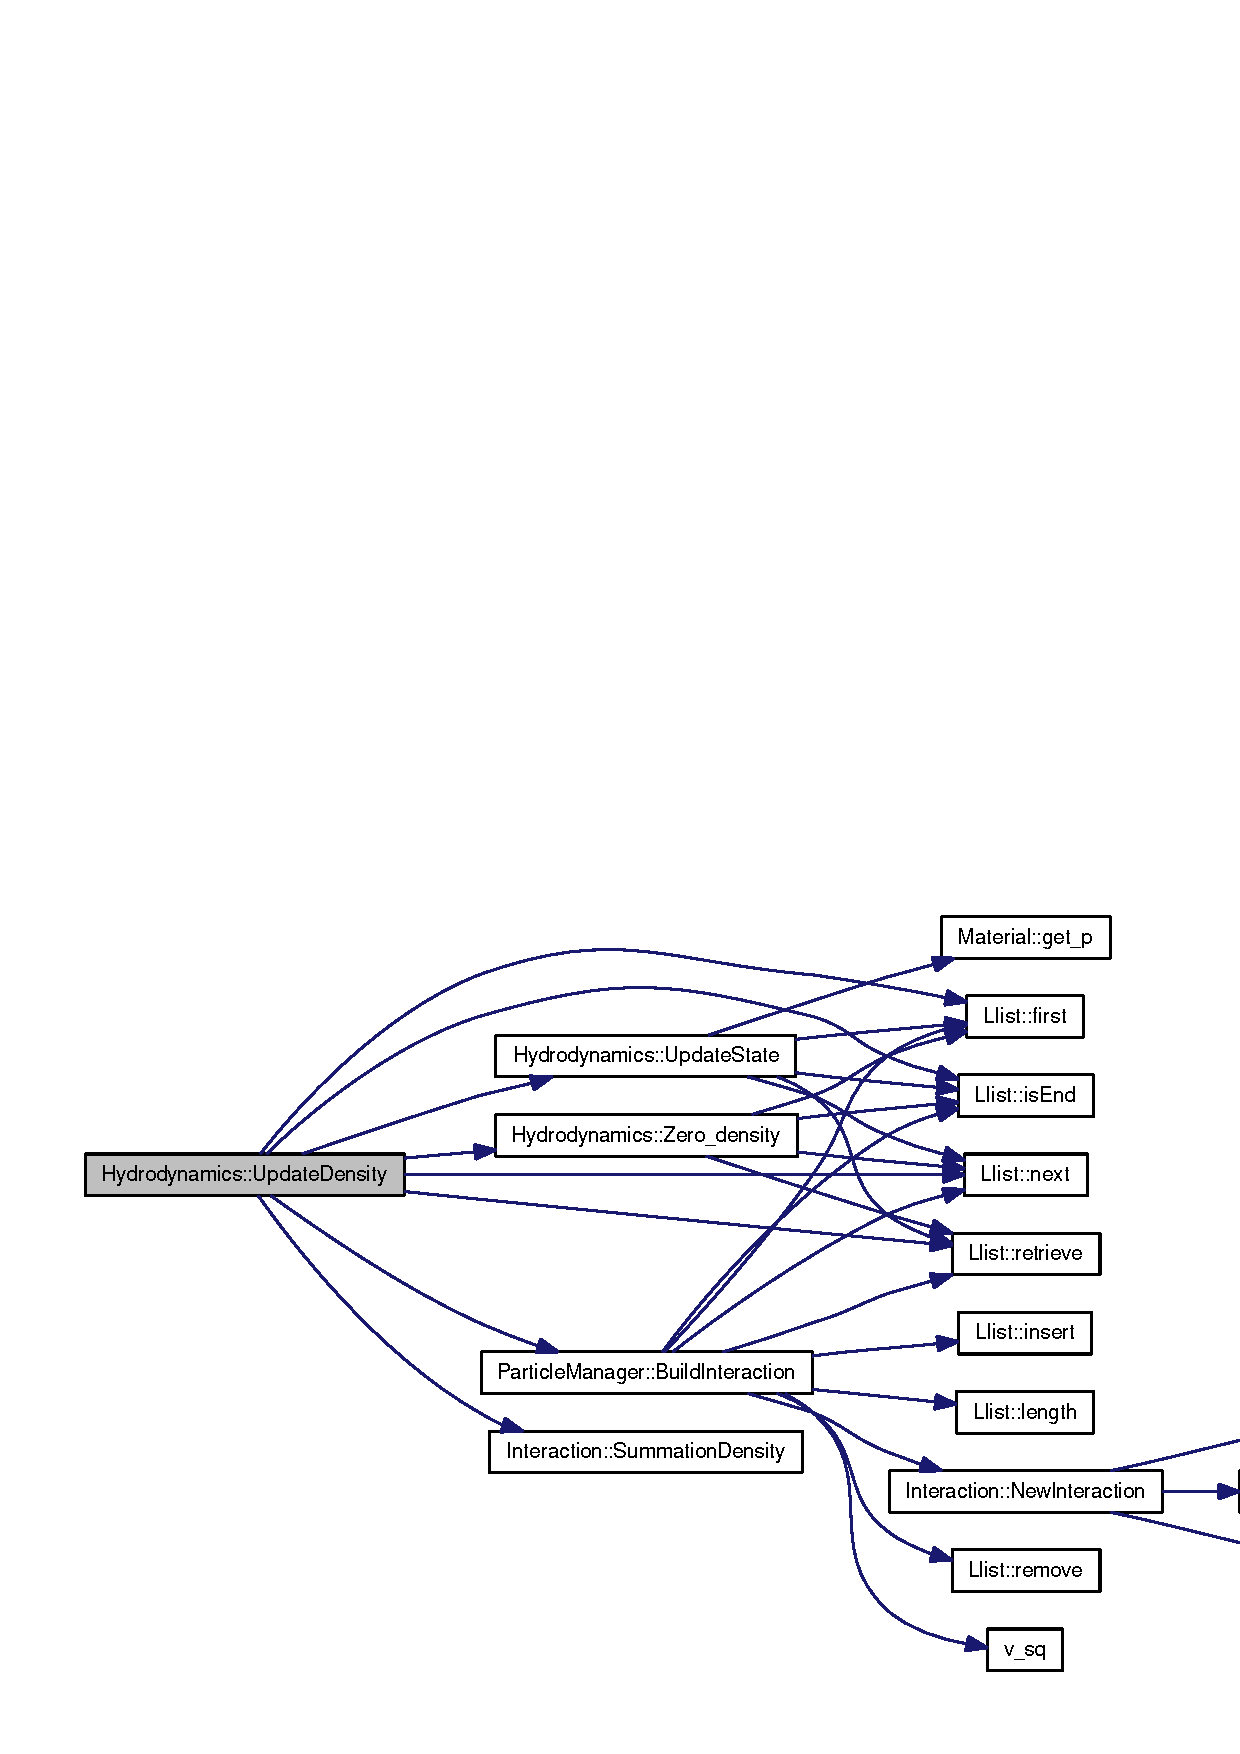
\includegraphics[width=352pt]{classHydrodynamics_1818eb1f9044ae980e92c70146e51c5b_cgraph}
\end{center}
\end{figure}


Here is the caller graph for this function:\nopagebreak
\begin{figure}[H]
\begin{center}
\leavevmode
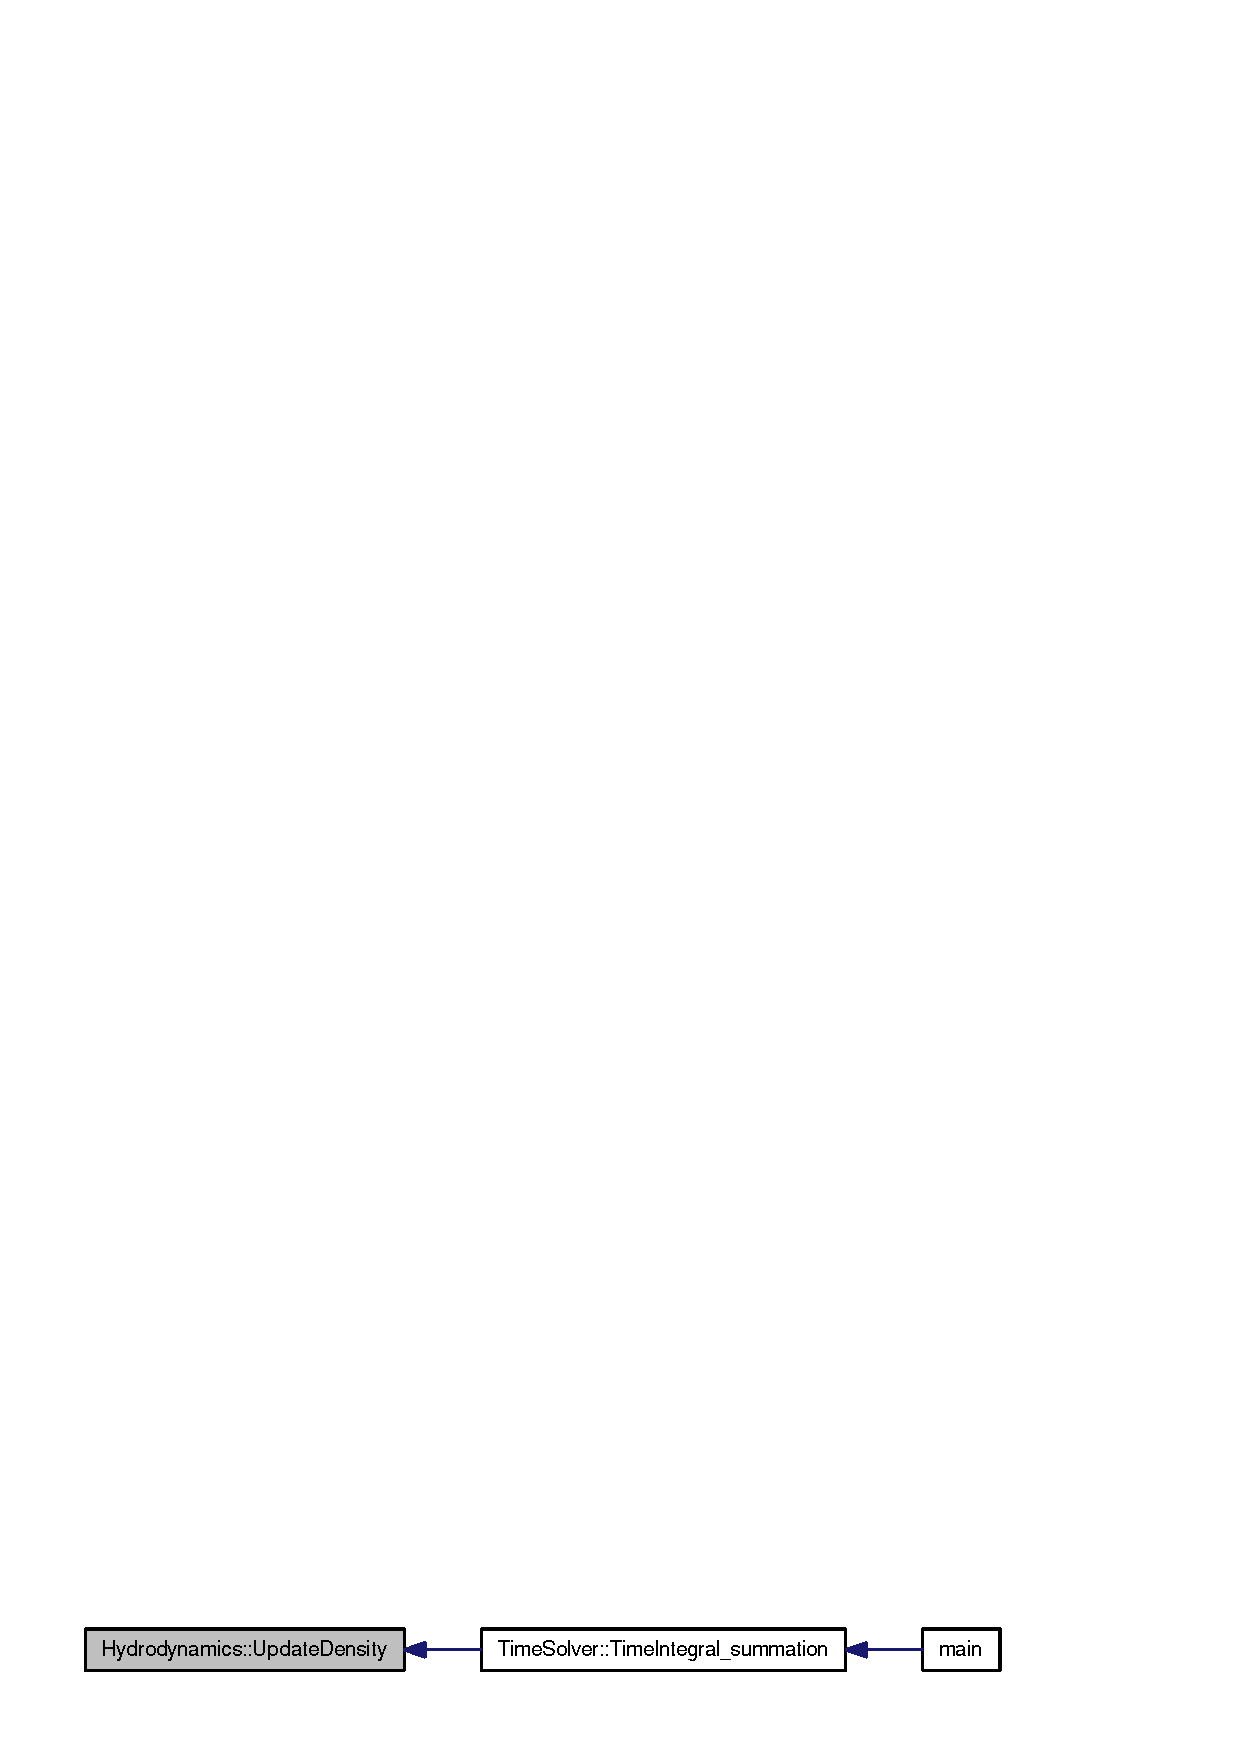
\includegraphics[width=242pt]{classHydrodynamics_1818eb1f9044ae980e92c70146e51c5b_icgraph}
\end{center}
\end{figure}
\hypertarget{classHydrodynamics_a755853b07cbbc5b484d78a3e787d1ef}{
\index{Hydrodynamics@{Hydrodynamics}!UpdatePahseMatrix@{UpdatePahseMatrix}}
\index{UpdatePahseMatrix@{UpdatePahseMatrix}!Hydrodynamics@{Hydrodynamics}}
\subsubsection[{UpdatePahseMatrix}]{\setlength{\rightskip}{0pt plus 5cm}void Hydrodynamics::UpdatePahseMatrix ({\bf Boundary} \& {\em boundary})}}
\label{classHydrodynamics_a755853b07cbbc5b484d78a3e787d1ef}


this method currently does {\bf NOTHING} 



\begin{itemize}
\item iterate particles on the real particle list\end{itemize}


\begin{itemize}
\item all phase surface stress (currently no action is performed)\end{itemize}


\begin{itemize}
\item iterate particles on the boundary particle list\end{itemize}


\begin{itemize}
\item all phase surface stress (currently no action is perforemd) \end{itemize}


Here is the call graph for this function:\nopagebreak
\begin{figure}[H]
\begin{center}
\leavevmode
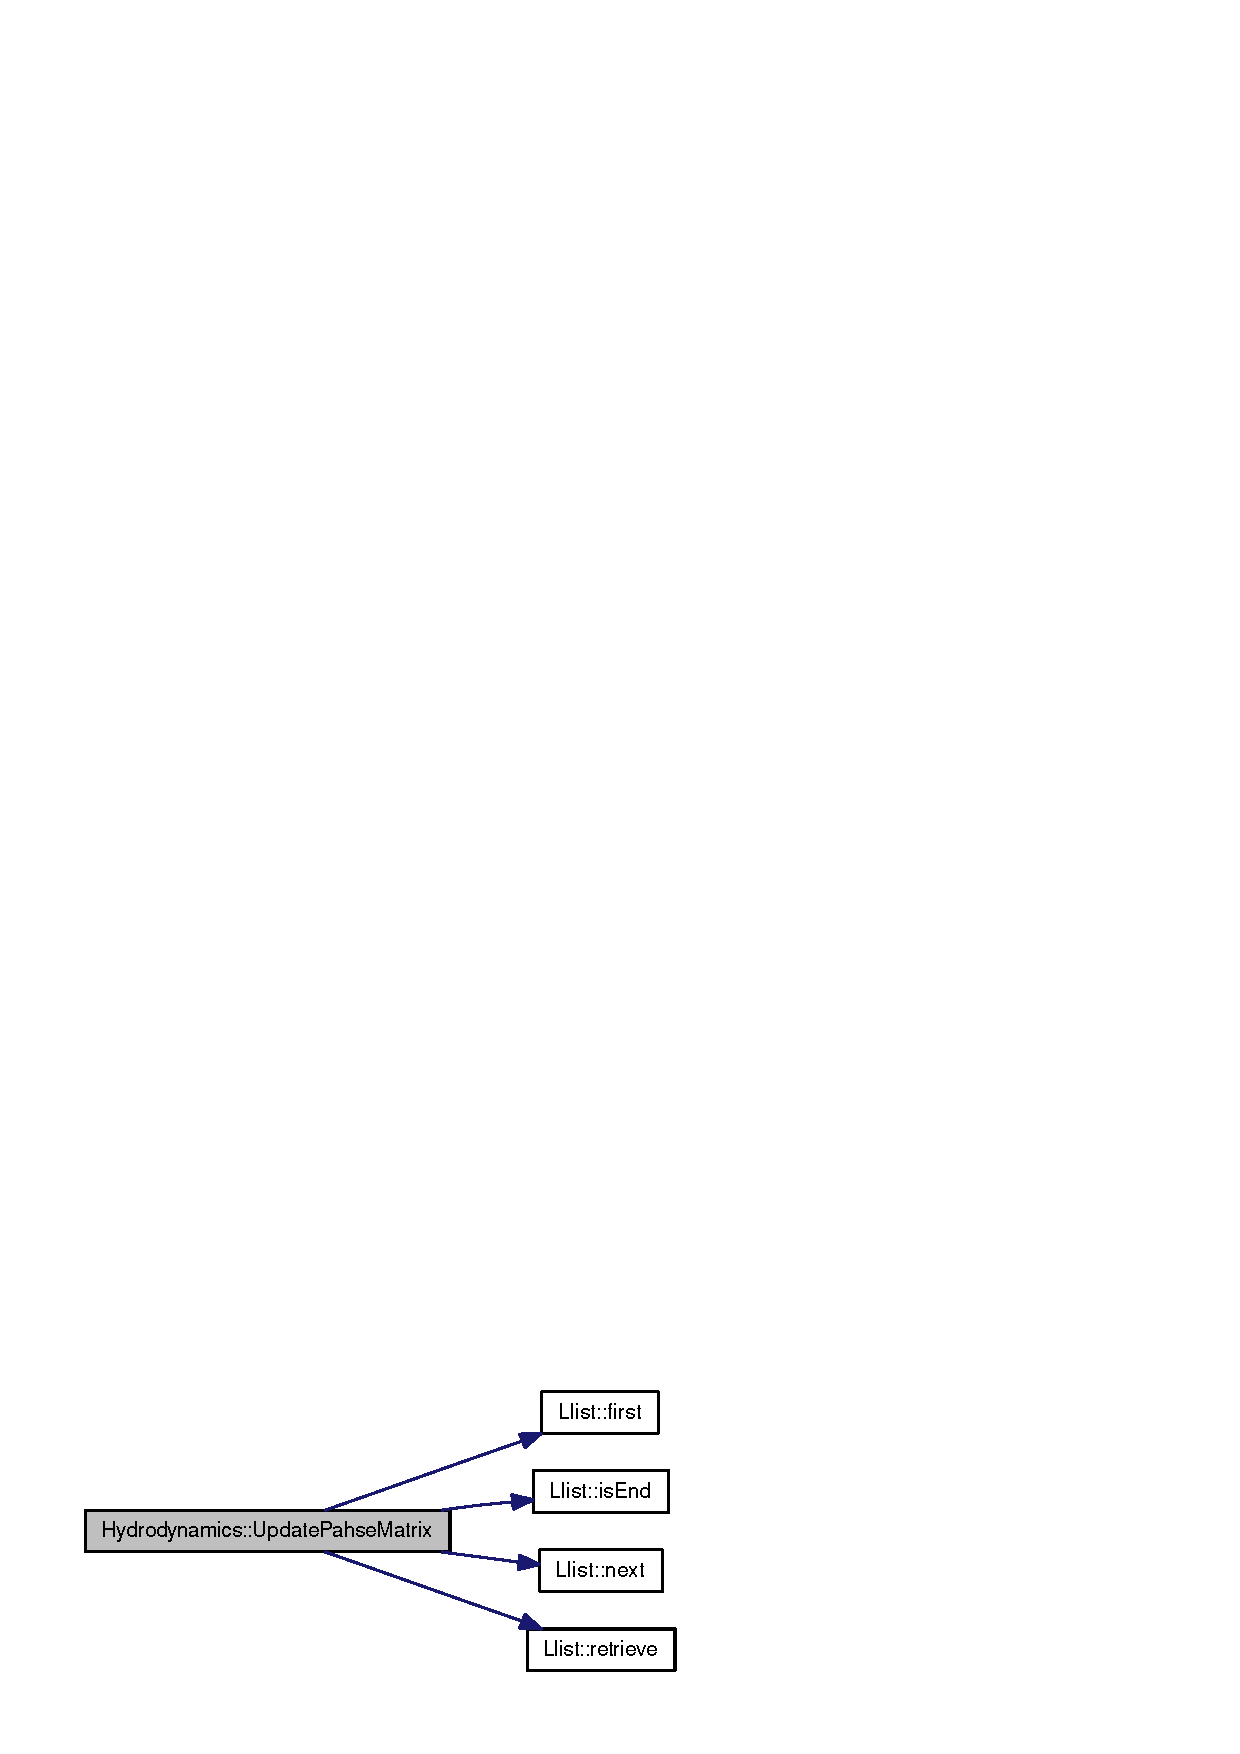
\includegraphics[width=164pt]{classHydrodynamics_a755853b07cbbc5b484d78a3e787d1ef_cgraph}
\end{center}
\end{figure}
\hypertarget{classHydrodynamics_cf0d749b11e8b8474dd204c6ea080235}{
\index{Hydrodynamics@{Hydrodynamics}!UpdatePair@{UpdatePair}}
\index{UpdatePair@{UpdatePair}!Hydrodynamics@{Hydrodynamics}}
\subsubsection[{UpdatePair}]{\setlength{\rightskip}{0pt plus 5cm}void Hydrodynamics::UpdatePair ({\bf QuinticSpline} \& {\em weight\_\-function})}}
\label{classHydrodynamics_cf0d749b11e8b8474dd204c6ea080235}


update new parameters in pairs 



\begin{itemize}
\item iterate the interaction list\end{itemize}


\begin{itemize}
\item and for each interactionpair call RenewInteraction method \end{itemize}


Here is the call graph for this function:\nopagebreak
\begin{figure}[H]
\begin{center}
\leavevmode
\includegraphics[width=251pt]{classHydrodynamics_cf0d749b11e8b8474dd204c6ea080235_cgraph}
\end{center}
\end{figure}


Here is the caller graph for this function:\nopagebreak
\begin{figure}[H]
\begin{center}
\leavevmode
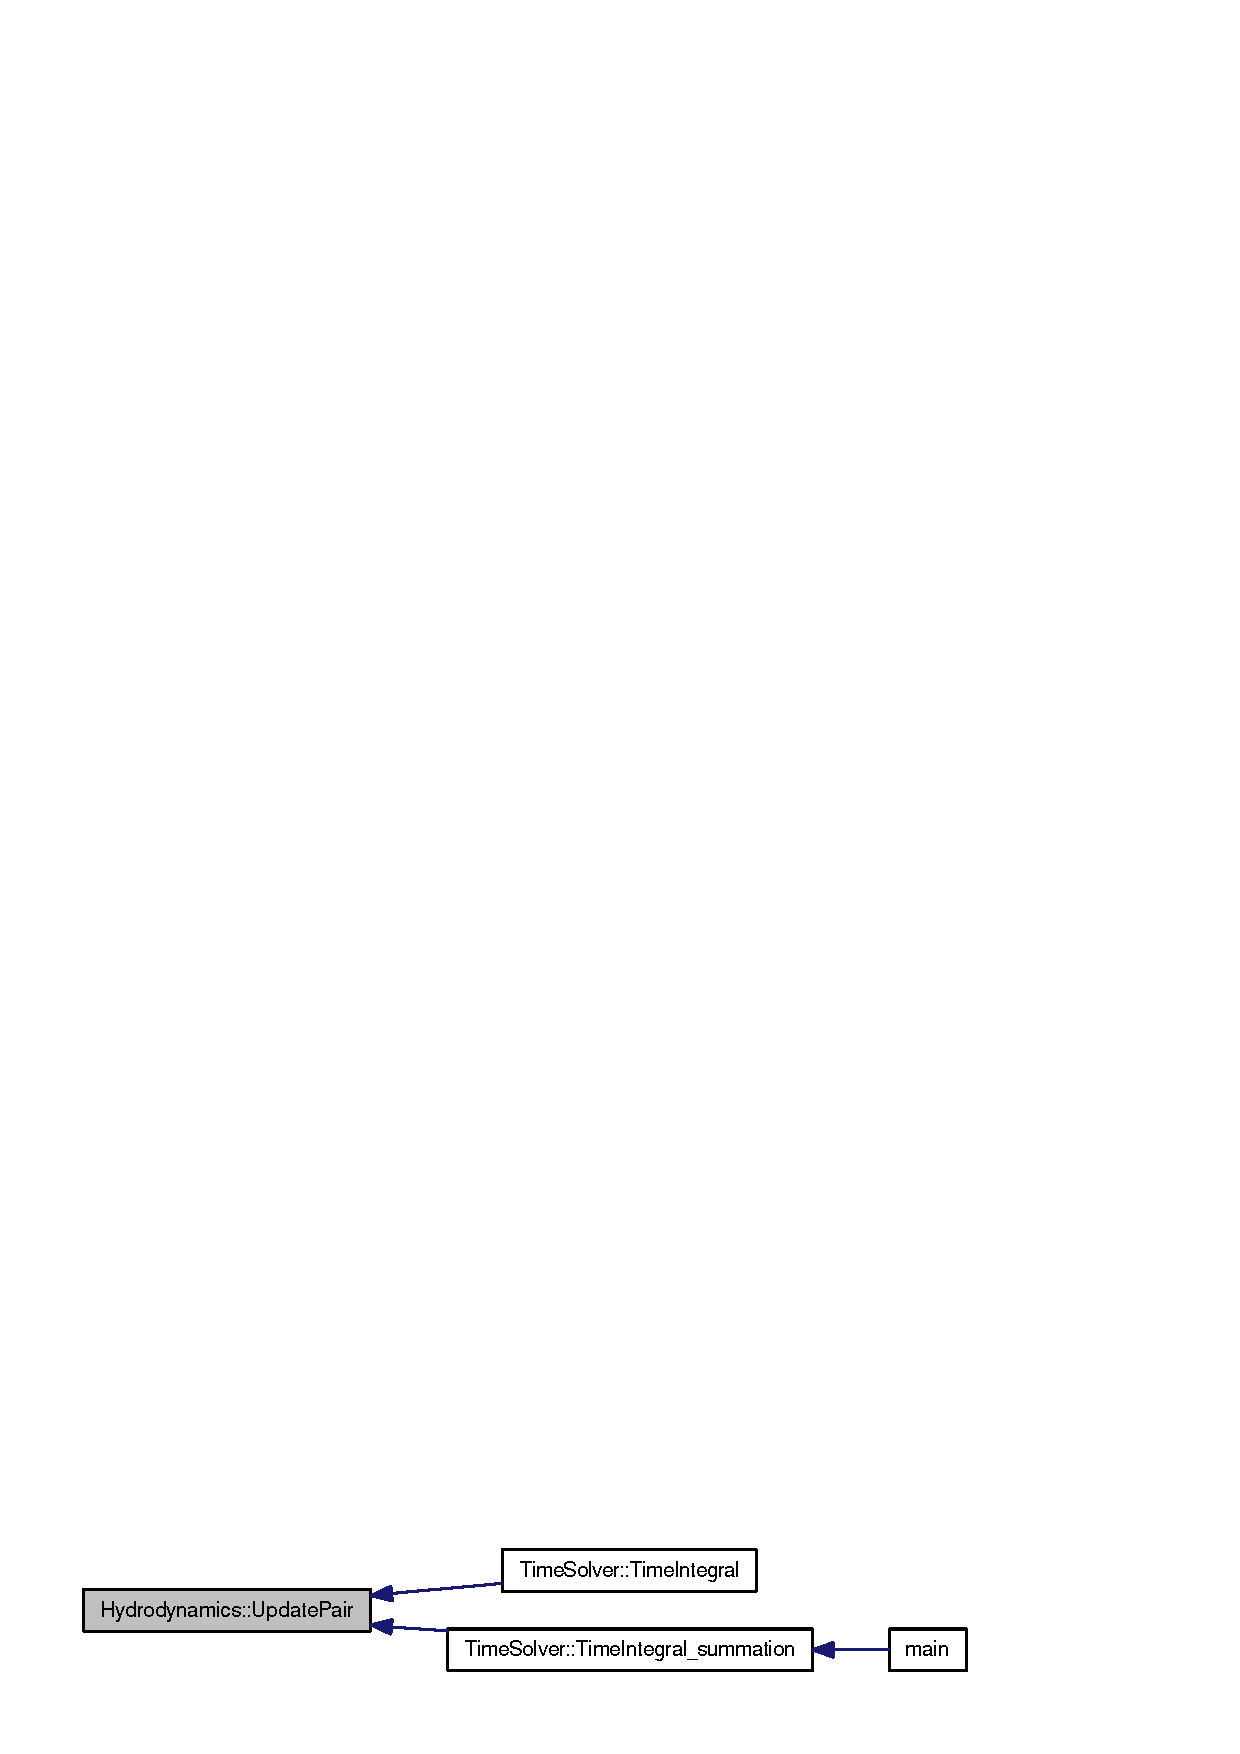
\includegraphics[width=234pt]{classHydrodynamics_cf0d749b11e8b8474dd204c6ea080235_icgraph}
\end{center}
\end{figure}
\hypertarget{classHydrodynamics_c87ff6437d540454ed7de2f726858f4a}{
\index{Hydrodynamics@{Hydrodynamics}!UpdatePhaseField@{UpdatePhaseField}}
\index{UpdatePhaseField@{UpdatePhaseField}!Hydrodynamics@{Hydrodynamics}}
\subsubsection[{UpdatePhaseField}]{\setlength{\rightskip}{0pt plus 5cm}void Hydrodynamics::UpdatePhaseField ({\bf Boundary} \& {\em boundary})}}
\label{classHydrodynamics_c87ff6437d540454ed7de2f726858f4a}




\begin{itemize}
\item initiate by calling \hyperlink{classHydrodynamics_dedab91b9a62eb7e26931cbbe73f79cc}{Zero\_\-PhaseField()}\end{itemize}


\begin{itemize}
\item iterate the interaction list\end{itemize}


\begin{itemize}
\item calculate for each pair the pair forces or change rate \end{itemize}


Here is the call graph for this function:\nopagebreak
\begin{figure}[H]
\begin{center}
\leavevmode
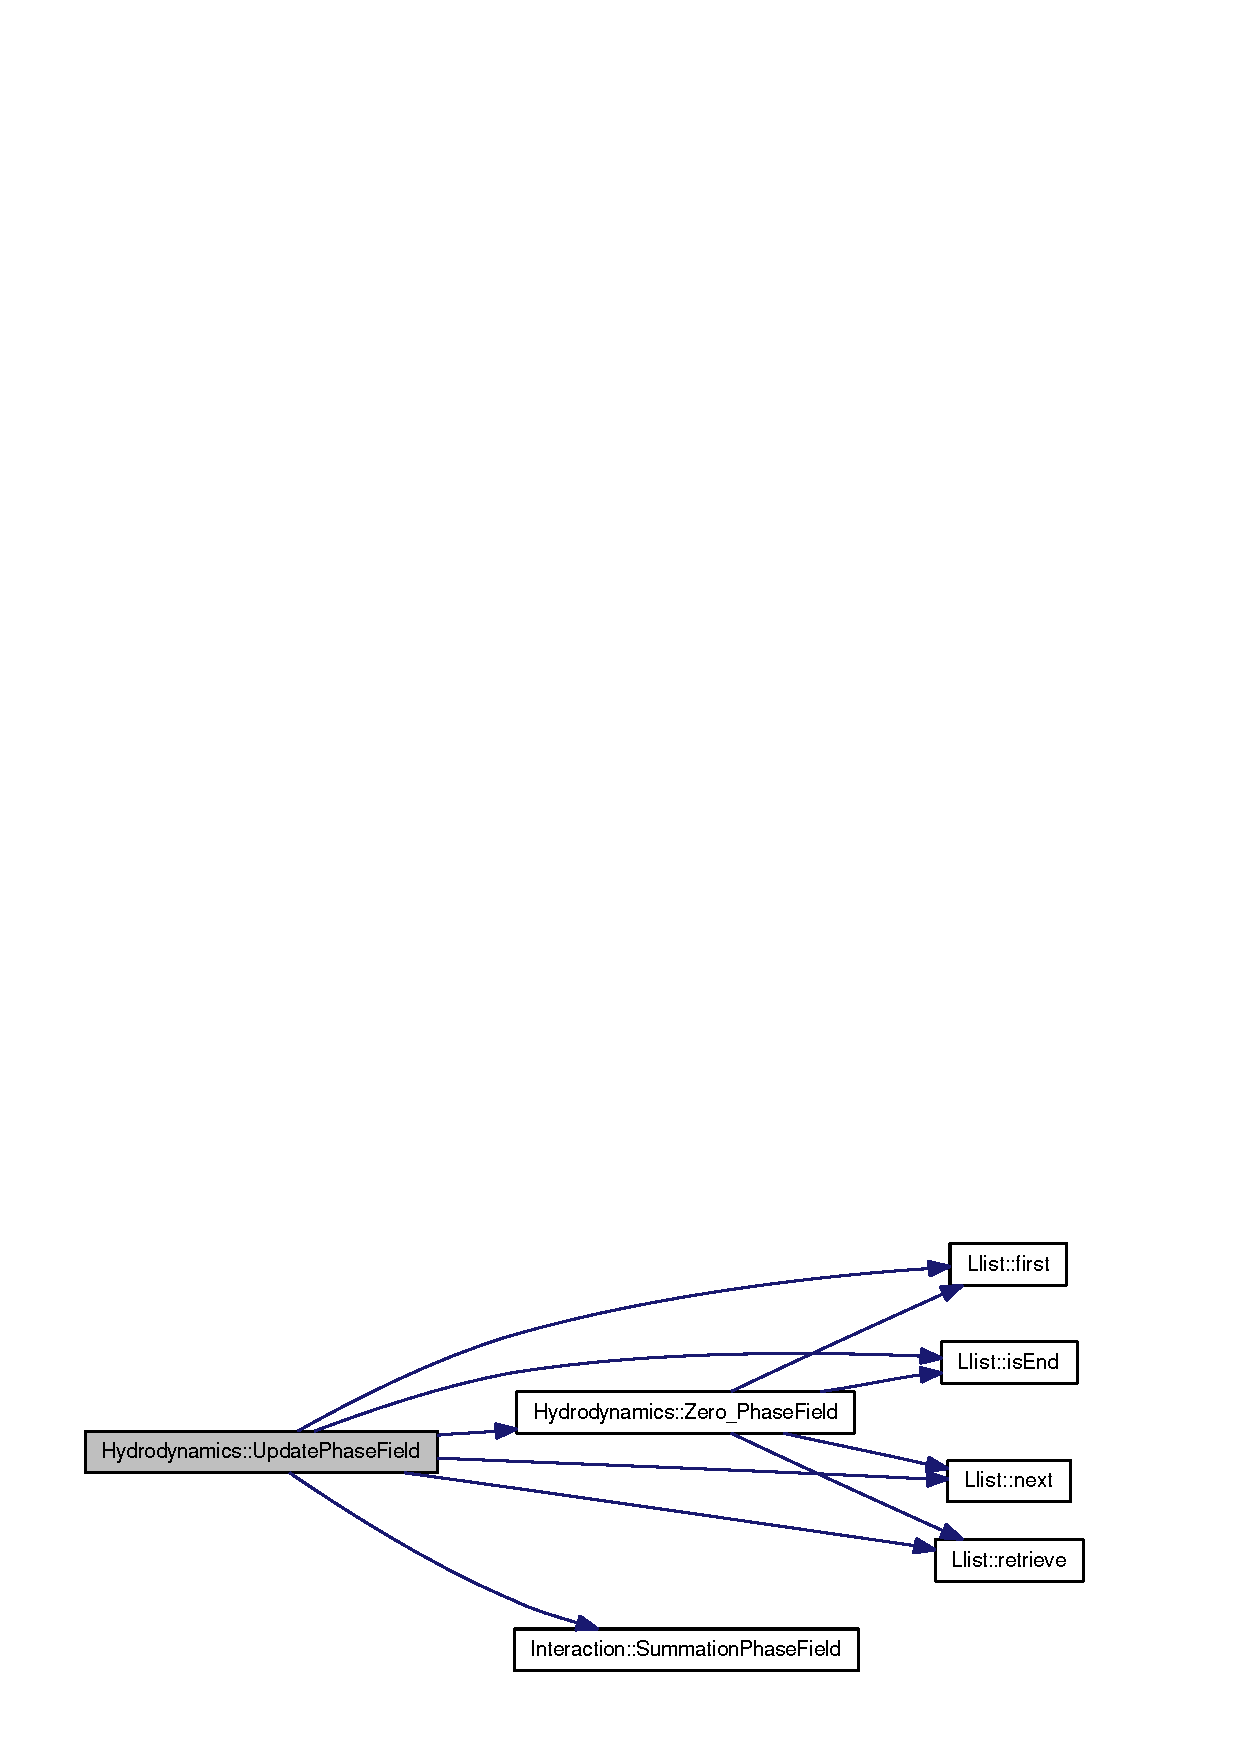
\includegraphics[width=262pt]{classHydrodynamics_c87ff6437d540454ed7de2f726858f4a_cgraph}
\end{center}
\end{figure}
\hypertarget{classHydrodynamics_939e9b2ec26b3e4a2eaf2683e5f0343d}{
\index{Hydrodynamics@{Hydrodynamics}!UpdatePhaseGradient@{UpdatePhaseGradient}}
\index{UpdatePhaseGradient@{UpdatePhaseGradient}!Hydrodynamics@{Hydrodynamics}}
\subsubsection[{UpdatePhaseGradient}]{\setlength{\rightskip}{0pt plus 5cm}void Hydrodynamics::UpdatePhaseGradient ({\bf Boundary} \& {\em boundary})}}
\label{classHydrodynamics_939e9b2ec26b3e4a2eaf2683e5f0343d}


not independant with UpdateDensity 



\begin{itemize}
\item initiate by callingZer\_\-PhaseGradient()\end{itemize}


\begin{itemize}
\item iterate the interaction list\end{itemize}


\begin{itemize}
\item calculate for each pair the pair forces or change rate \end{itemize}


Here is the call graph for this function:\nopagebreak
\begin{figure}[H]
\begin{center}
\leavevmode
\includegraphics[width=278pt]{classHydrodynamics_939e9b2ec26b3e4a2eaf2683e5f0343d_cgraph}
\end{center}
\end{figure}


Here is the caller graph for this function:\nopagebreak
\begin{figure}[H]
\begin{center}
\leavevmode
\includegraphics[width=258pt]{classHydrodynamics_939e9b2ec26b3e4a2eaf2683e5f0343d_icgraph}
\end{center}
\end{figure}
\hypertarget{classHydrodynamics_dbbe86fd4eac49912a9ffb5e284883ee}{
\index{Hydrodynamics@{Hydrodynamics}!UpdatePhaseLaplacian@{UpdatePhaseLaplacian}}
\index{UpdatePhaseLaplacian@{UpdatePhaseLaplacian}!Hydrodynamics@{Hydrodynamics}}
\subsubsection[{UpdatePhaseLaplacian}]{\setlength{\rightskip}{0pt plus 5cm}void Hydrodynamics::UpdatePhaseLaplacian ({\bf Boundary} \& {\em boundary})}}
\label{classHydrodynamics_dbbe86fd4eac49912a9ffb5e284883ee}




\begin{itemize}
\item initiate zero shear rateby calling \hyperlink{classHydrodynamics_d1c5fd5b500eacb886a72f2dab13e91b}{Zero\_\-PhaseLaplacian()}\end{itemize}


\begin{itemize}
\item iterate the interaction list\end{itemize}


\begin{itemize}
\item calculate for each pair the pair forces or change rate \end{itemize}


Here is the call graph for this function:\nopagebreak
\begin{figure}[H]
\begin{center}
\leavevmode
\includegraphics[width=281pt]{classHydrodynamics_dbbe86fd4eac49912a9ffb5e284883ee_cgraph}
\end{center}
\end{figure}
\hypertarget{classHydrodynamics_49570aaeedea32d7a2baf0532880b2e8}{
\index{Hydrodynamics@{Hydrodynamics}!UpdateShearRate@{UpdateShearRate}}
\index{UpdateShearRate@{UpdateShearRate}!Hydrodynamics@{Hydrodynamics}}
\subsubsection[{UpdateShearRate}]{\setlength{\rightskip}{0pt plus 5cm}void Hydrodynamics::UpdateShearRate ()}}
\label{classHydrodynamics_49570aaeedea32d7a2baf0532880b2e8}


??? 



\begin{itemize}
\item initiate by calling Zero\_\-ShearRate(\end{itemize}


\begin{itemize}
\item iterate the interaction list\end{itemize}


\begin{itemize}
\item calculate for each pair the pair forces or change rate \end{itemize}


Here is the call graph for this function:\nopagebreak
\begin{figure}[H]
\begin{center}
\leavevmode
\includegraphics[width=258pt]{classHydrodynamics_49570aaeedea32d7a2baf0532880b2e8_cgraph}
\end{center}
\end{figure}
\hypertarget{classHydrodynamics_7ae4f1005699f13414ec6c487bac0ee0}{
\index{Hydrodynamics@{Hydrodynamics}!UpdateShearRate@{UpdateShearRate}}
\index{UpdateShearRate@{UpdateShearRate}!Hydrodynamics@{Hydrodynamics}}
\subsubsection[{UpdateShearRate}]{\setlength{\rightskip}{0pt plus 5cm}void Hydrodynamics::UpdateShearRate ({\bf ParticleManager} \& {\em particles}, \/  {\bf QuinticSpline} \& {\em weight\_\-function})}}
\label{classHydrodynamics_7ae4f1005699f13414ec6c487bac0ee0}


summation for shear rates (with updating interaction list) 



\begin{itemize}
\item obtain the interaction pairs\end{itemize}


\begin{itemize}
\item initiate by calling Zero\_\-ShearRate Method\end{itemize}


\begin{itemize}
\item iterate the interaction list\end{itemize}


\begin{itemize}
\item calculate for each pair the pair forces or change rate \end{itemize}


Here is the call graph for this function:\nopagebreak
\begin{figure}[H]
\begin{center}
\leavevmode
\includegraphics[width=359pt]{classHydrodynamics_7ae4f1005699f13414ec6c487bac0ee0_cgraph}
\end{center}
\end{figure}
\hypertarget{classHydrodynamics_1698dbe8ecc0e730319de5d7eca7a891}{
\index{Hydrodynamics@{Hydrodynamics}!UpdateState@{UpdateState}}
\index{UpdateState@{UpdateState}!Hydrodynamics@{Hydrodynamics}}
\subsubsection[{UpdateState}]{\setlength{\rightskip}{0pt plus 5cm}void Hydrodynamics::UpdateState ()}}
\label{classHydrodynamics_1698dbe8ecc0e730319de5d7eca7a891}


calculate states from conservatives 



\begin{itemize}
\item iterate particles on the real particle list\end{itemize}


\begin{itemize}
\item calculate pressure for each particle \end{itemize}


Here is the call graph for this function:\nopagebreak
\begin{figure}[H]
\begin{center}
\leavevmode
\includegraphics[width=153pt]{classHydrodynamics_1698dbe8ecc0e730319de5d7eca7a891_cgraph}
\end{center}
\end{figure}


Here is the caller graph for this function:\nopagebreak
\begin{figure}[H]
\begin{center}
\leavevmode
\includegraphics[width=332pt]{classHydrodynamics_1698dbe8ecc0e730319de5d7eca7a891_icgraph}
\end{center}
\end{figure}
\hypertarget{classHydrodynamics_f5b2c4ad14824e4b6192faa6f60f4014}{
\index{Hydrodynamics@{Hydrodynamics}!UpdateSurfaceStress@{UpdateSurfaceStress}}
\index{UpdateSurfaceStress@{UpdateSurfaceStress}!Hydrodynamics@{Hydrodynamics}}
\subsubsection[{UpdateSurfaceStress}]{\setlength{\rightskip}{0pt plus 5cm}void Hydrodynamics::UpdateSurfaceStress ({\bf Boundary} \& {\em boundary})}}
\label{classHydrodynamics_f5b2c4ad14824e4b6192faa6f60f4014}




\begin{itemize}
\item iterate particles on the real particle list\end{itemize}


\begin{itemize}
\item update phase surface stress for all particles on this list\end{itemize}


\begin{itemize}
\item iterate particles on the boundary particle list\end{itemize}


\begin{itemize}
\item update phase surface stress for all particles on this list \end{itemize}


Here is the call graph for this function:\nopagebreak
\begin{figure}[H]
\begin{center}
\leavevmode
\includegraphics[width=167pt]{classHydrodynamics_f5b2c4ad14824e4b6192faa6f60f4014_cgraph}
\end{center}
\end{figure}


Here is the caller graph for this function:\nopagebreak
\begin{figure}[H]
\begin{center}
\leavevmode
\includegraphics[width=256pt]{classHydrodynamics_f5b2c4ad14824e4b6192faa6f60f4014_icgraph}
\end{center}
\end{figure}
\hypertarget{classHydrodynamics_09a3f5a5c055e0efc822fdf80f40cd7d}{
\index{Hydrodynamics@{Hydrodynamics}!UpdateVolume@{UpdateVolume}}
\index{UpdateVolume@{UpdateVolume}!Hydrodynamics@{Hydrodynamics}}
\subsubsection[{UpdateVolume}]{\setlength{\rightskip}{0pt plus 5cm}void Hydrodynamics::UpdateVolume ({\bf ParticleManager} \& {\em particles}, \/  {\bf QuinticSpline} \& {\em weight\_\-function})}}
\label{classHydrodynamics_09a3f5a5c055e0efc822fdf80f40cd7d}


calculate partilce volume 



\begin{itemize}
\item iterate particles on the particle list

\begin{itemize}
\item take origin particle

\begin{itemize}
\item sum the weights for all of these particles (because they are the inverse of a volume!?!)\end{itemize}


\item clear the NNP\_\-list\end{itemize}
\end{itemize}


Here is the call graph for this function:\nopagebreak
\begin{figure}[H]
\begin{center}
\leavevmode
\includegraphics[width=246pt]{classHydrodynamics_09a3f5a5c055e0efc822fdf80f40cd7d_cgraph}
\end{center}
\end{figure}
\hypertarget{classHydrodynamics_13810b3b4110a2b931bf7426af2f9bcf}{
\index{Hydrodynamics@{Hydrodynamics}!Zero\_\-density@{Zero\_\-density}}
\index{Zero\_\-density@{Zero\_\-density}!Hydrodynamics@{Hydrodynamics}}
\subsubsection[{Zero\_\-density}]{\setlength{\rightskip}{0pt plus 5cm}void Hydrodynamics::Zero\_\-density ()}}
\label{classHydrodynamics_13810b3b4110a2b931bf7426af2f9bcf}


initiate particle density to zero 



\begin{itemize}
\item iterate particles on the real particle list\end{itemize}


\begin{itemize}
\item set for each particle density to zero \end{itemize}


Here is the call graph for this function:\nopagebreak
\begin{figure}[H]
\begin{center}
\leavevmode
\includegraphics[width=149pt]{classHydrodynamics_13810b3b4110a2b931bf7426af2f9bcf_cgraph}
\end{center}
\end{figure}


Here is the caller graph for this function:\nopagebreak
\begin{figure}[H]
\begin{center}
\leavevmode
\includegraphics[width=333pt]{classHydrodynamics_13810b3b4110a2b931bf7426af2f9bcf_icgraph}
\end{center}
\end{figure}
\hypertarget{classHydrodynamics_dedab91b9a62eb7e26931cbbe73f79cc}{
\index{Hydrodynamics@{Hydrodynamics}!Zero\_\-PhaseField@{Zero\_\-PhaseField}}
\index{Zero\_\-PhaseField@{Zero\_\-PhaseField}!Hydrodynamics@{Hydrodynamics}}
\subsubsection[{Zero\_\-PhaseField}]{\setlength{\rightskip}{0pt plus 5cm}void Hydrodynamics::Zero\_\-PhaseField ({\bf Boundary} \& {\em boundary})}}
\label{classHydrodynamics_dedab91b9a62eb7e26931cbbe73f79cc}




\begin{itemize}
\item iterate particles on the real particle list\end{itemize}


\begin{itemize}
\item set all phases for all of these particles to zero\end{itemize}


\begin{itemize}
\item iterate particles on the boundary particle list\end{itemize}


\begin{itemize}
\item set all phases for all of these particles to zero \end{itemize}


Here is the call graph for this function:\nopagebreak
\begin{figure}[H]
\begin{center}
\leavevmode
\includegraphics[width=157pt]{classHydrodynamics_dedab91b9a62eb7e26931cbbe73f79cc_cgraph}
\end{center}
\end{figure}


Here is the caller graph for this function:\nopagebreak
\begin{figure}[H]
\begin{center}
\leavevmode
\includegraphics[width=206pt]{classHydrodynamics_dedab91b9a62eb7e26931cbbe73f79cc_icgraph}
\end{center}
\end{figure}
\hypertarget{classHydrodynamics_3c9019f19ccac5370b7b0ccda343b5d2}{
\index{Hydrodynamics@{Hydrodynamics}!Zero\_\-PhaseGradient@{Zero\_\-PhaseGradient}}
\index{Zero\_\-PhaseGradient@{Zero\_\-PhaseGradient}!Hydrodynamics@{Hydrodynamics}}
\subsubsection[{Zero\_\-PhaseGradient}]{\setlength{\rightskip}{0pt plus 5cm}void Hydrodynamics::Zero\_\-PhaseGradient ({\bf Boundary} \& {\em boundary})}}
\label{classHydrodynamics_3c9019f19ccac5370b7b0ccda343b5d2}




\begin{itemize}
\item iterate particles on the real particle list\end{itemize}


\begin{itemize}
\item set phase gradient to zeo for each of these particles\end{itemize}


\begin{itemize}
\item iterate particles on the boundary particle list\end{itemize}


\begin{itemize}
\item set phase gradient to zeo for each of these particle \end{itemize}


Here is the call graph for this function:\nopagebreak
\begin{figure}[H]
\begin{center}
\leavevmode
\includegraphics[width=165pt]{classHydrodynamics_3c9019f19ccac5370b7b0ccda343b5d2_cgraph}
\end{center}
\end{figure}


Here is the caller graph for this function:\nopagebreak
\begin{figure}[H]
\begin{center}
\leavevmode
\includegraphics[width=365pt]{classHydrodynamics_3c9019f19ccac5370b7b0ccda343b5d2_icgraph}
\end{center}
\end{figure}
\hypertarget{classHydrodynamics_d1c5fd5b500eacb886a72f2dab13e91b}{
\index{Hydrodynamics@{Hydrodynamics}!Zero\_\-PhaseLaplacian@{Zero\_\-PhaseLaplacian}}
\index{Zero\_\-PhaseLaplacian@{Zero\_\-PhaseLaplacian}!Hydrodynamics@{Hydrodynamics}}
\subsubsection[{Zero\_\-PhaseLaplacian}]{\setlength{\rightskip}{0pt plus 5cm}void Hydrodynamics::Zero\_\-PhaseLaplacian ({\bf Boundary} \& {\em boundary})}}
\label{classHydrodynamics_d1c5fd5b500eacb886a72f2dab13e91b}




\begin{itemize}
\item iterate particles on the real particle list\end{itemize}


\begin{itemize}
\item set to zero all phase Laplacians for these particles\end{itemize}


\begin{itemize}
\item iterate particles on the boundary particle list\end{itemize}


\begin{itemize}
\item set to zero all phase Laplacians for these particles \end{itemize}


Here is the call graph for this function:\nopagebreak
\begin{figure}[H]
\begin{center}
\leavevmode
\includegraphics[width=168pt]{classHydrodynamics_d1c5fd5b500eacb886a72f2dab13e91b_cgraph}
\end{center}
\end{figure}


Here is the caller graph for this function:\nopagebreak
\begin{figure}[H]
\begin{center}
\leavevmode
\includegraphics[width=227pt]{classHydrodynamics_d1c5fd5b500eacb886a72f2dab13e91b_icgraph}
\end{center}
\end{figure}
\hypertarget{classHydrodynamics_f67579320cbdccaf49bbdf3dfb13f23c}{
\index{Hydrodynamics@{Hydrodynamics}!Zero\_\-Random@{Zero\_\-Random}}
\index{Zero\_\-Random@{Zero\_\-Random}!Hydrodynamics@{Hydrodynamics}}
\subsubsection[{Zero\_\-Random}]{\setlength{\rightskip}{0pt plus 5cm}void Hydrodynamics::Zero\_\-Random ()}}
\label{classHydrodynamics_f67579320cbdccaf49bbdf3dfb13f23c}


initiate random force (DPD simulation) 



\begin{itemize}
\item iterate particles on the real particle list\end{itemize}


\begin{itemize}
\item all random values to zero (so, \_\-dU is random value???) \end{itemize}


Here is the call graph for this function:\nopagebreak
\begin{figure}[H]
\begin{center}
\leavevmode
\includegraphics[width=151pt]{classHydrodynamics_f67579320cbdccaf49bbdf3dfb13f23c_cgraph}
\end{center}
\end{figure}


Here is the caller graph for this function:\nopagebreak
\begin{figure}[H]
\begin{center}
\leavevmode
\includegraphics[width=272pt]{classHydrodynamics_f67579320cbdccaf49bbdf3dfb13f23c_icgraph}
\end{center}
\end{figure}
\hypertarget{classHydrodynamics_049f88c2f97863edae4489618dc9e853}{
\index{Hydrodynamics@{Hydrodynamics}!Zero\_\-ShearRate@{Zero\_\-ShearRate}}
\index{Zero\_\-ShearRate@{Zero\_\-ShearRate}!Hydrodynamics@{Hydrodynamics}}
\subsubsection[{Zero\_\-ShearRate}]{\setlength{\rightskip}{0pt plus 5cm}void Hydrodynamics::Zero\_\-ShearRate ()}}
\label{classHydrodynamics_049f88c2f97863edae4489618dc9e853}




\begin{itemize}
\item iterate particles on the real particle list\end{itemize}


\begin{itemize}
\item set ShearRate to zero for each particle \end{itemize}


Here is the call graph for this function:\nopagebreak
\begin{figure}[H]
\begin{center}
\leavevmode
\includegraphics[width=156pt]{classHydrodynamics_049f88c2f97863edae4489618dc9e853_cgraph}
\end{center}
\end{figure}


Here is the caller graph for this function:\nopagebreak
\begin{figure}[H]
\begin{center}
\leavevmode
\includegraphics[width=203pt]{classHydrodynamics_049f88c2f97863edae4489618dc9e853_icgraph}
\end{center}
\end{figure}
\hypertarget{classHydrodynamics_4f65196eb3002238371d0e04dd76c02a}{
\index{Hydrodynamics@{Hydrodynamics}!Zero\_\-Velocity@{Zero\_\-Velocity}}
\index{Zero\_\-Velocity@{Zero\_\-Velocity}!Hydrodynamics@{Hydrodynamics}}
\subsubsection[{Zero\_\-Velocity}]{\setlength{\rightskip}{0pt plus 5cm}void Hydrodynamics::Zero\_\-Velocity ()}}
\label{classHydrodynamics_4f65196eb3002238371d0e04dd76c02a}


special uitilities 



\begin{itemize}
\item iterate particles on the real particle list\end{itemize}


\begin{itemize}
\item all velocities to zero \end{itemize}


Here is the call graph for this function:\nopagebreak
\begin{figure}[H]
\begin{center}
\leavevmode
\includegraphics[width=151pt]{classHydrodynamics_4f65196eb3002238371d0e04dd76c02a_cgraph}
\end{center}
\end{figure}
\hypertarget{classHydrodynamics_67e2d72d69156a086d43168f5cd58bf7}{
\index{Hydrodynamics@{Hydrodynamics}!ZeroChangeRate@{ZeroChangeRate}}
\index{ZeroChangeRate@{ZeroChangeRate}!Hydrodynamics@{Hydrodynamics}}
\subsubsection[{ZeroChangeRate}]{\setlength{\rightskip}{0pt plus 5cm}void Hydrodynamics::ZeroChangeRate ()}}
\label{classHydrodynamics_67e2d72d69156a086d43168f5cd58bf7}


initiate particle change rate 



\begin{itemize}
\item iterate particles on the real particle list\end{itemize}


\begin{itemize}
\item set for each particle change rates to zero \end{itemize}


Here is the call graph for this function:\nopagebreak
\begin{figure}[H]
\begin{center}
\leavevmode
\includegraphics[width=157pt]{classHydrodynamics_67e2d72d69156a086d43168f5cd58bf7_cgraph}
\end{center}
\end{figure}


Here is the caller graph for this function:\nopagebreak
\begin{figure}[H]
\begin{center}
\leavevmode
\includegraphics[width=351pt]{classHydrodynamics_67e2d72d69156a086d43168f5cd58bf7_icgraph}
\end{center}
\end{figure}


The documentation for this class was generated from the following files:\begin{CompactItemize}
\item 
\hyperlink{hydrodynamics_8h}{hydrodynamics.h}\item 
\hyperlink{hydrodynamics_8cpp}{hydrodynamics.cpp}\end{CompactItemize}

\hypertarget{classInitiation}{
\section{Initiation Class Reference}
\label{classInitiation}\index{Initiation@{Initiation}}
}
Initiates the simulation.  


{\tt \#include $<$initiation.h$>$}

\subsection*{Public Member Functions}
\begin{CompactItemize}
\item 
\hyperlink{classInitiation_4db3b8c45d38cf4e188de6aa672e8c0d}{Initiation} (const char $\ast$project\_\-name)
\item 
void \hyperlink{classInitiation_916e5b3e316dad1f524a1327b9e4aeb4}{non\_\-dimensionalize} ()
\begin{CompactList}\small\item\em non-dimensionalize initial condition and parameters \item\end{CompactList}\item 
void \hyperlink{classInitiation_cdbf1374b9b0f0b50a0bb1d9abf76293}{show\_\-information} ()
\begin{CompactList}\small\item\em show information on screen \item\end{CompactList}\item 
void \hyperlink{classInitiation_e80adc7d2105ad67b766fd1127966df3}{VolumeMass} (\hyperlink{classHydrodynamics}{Hydrodynamics} \&hydro, \hyperlink{classParticleManager}{ParticleManager} \&particles, \hyperlink{classQuinticSpline}{QuinticSpline} \&weight\_\-function)
\begin{CompactList}\small\item\em predict the particle volume and mass \item\end{CompactList}\item 
\hypertarget{classInitiation_689c73dd7149dc11207eca5c3109a7cd}{
double \hyperlink{classInitiation_689c73dd7149dc11207eca5c3109a7cd}{non\_\-dms\_\-p} (double p)}
\label{classInitiation_689c73dd7149dc11207eca5c3109a7cd}

\begin{CompactList}\small\item\em a non dimensionalize method \item\end{CompactList}\item 
\hypertarget{classInitiation_deddac317c4755623e4fcef187b3f07a}{
double \hyperlink{classInitiation_deddac317c4755623e4fcef187b3f07a}{non\_\-dms\_\-T} (double T)}
\label{classInitiation_deddac317c4755623e4fcef187b3f07a}

\begin{CompactList}\small\item\em a non dimensionalize method \item\end{CompactList}\item 
\hypertarget{classInitiation_29245385c400c4f0de40707cb07dc0dd}{
double \hyperlink{classInitiation_29245385c400c4f0de40707cb07dc0dd}{non\_\-dms\_\-rho} (double rho)}
\label{classInitiation_29245385c400c4f0de40707cb07dc0dd}

\begin{CompactList}\small\item\em a non dimensionalize method \item\end{CompactList}\item 
\hypertarget{classInitiation_e39448af30a53dd8f4354492be9883fc}{
double \hyperlink{classInitiation_e39448af30a53dd8f4354492be9883fc}{non\_\-dms\_\-mass} (double mass)}
\label{classInitiation_e39448af30a53dd8f4354492be9883fc}

\begin{CompactList}\small\item\em a non dimensionalize method \item\end{CompactList}\item 
\hypertarget{classInitiation_2ec28f27a197bfaeb3937733dbb47b03}{
double \hyperlink{classInitiation_2ec28f27a197bfaeb3937733dbb47b03}{non\_\-dms\_\-time} (double time)}
\label{classInitiation_2ec28f27a197bfaeb3937733dbb47b03}

\begin{CompactList}\small\item\em a non dimensionalize method \item\end{CompactList}\item 
\hypertarget{classInitiation_921fe74dff7653520c5e72cc5c11b353}{
double \hyperlink{classInitiation_921fe74dff7653520c5e72cc5c11b353}{non\_\-dms\_\-length} (double length)}
\label{classInitiation_921fe74dff7653520c5e72cc5c11b353}

\begin{CompactList}\small\item\em a non dimensionalize method \item\end{CompactList}\item 
\hypertarget{classInitiation_1b13c381a36c5d841bf9b4dc108a03f6}{
Vec2d \hyperlink{classInitiation_1b13c381a36c5d841bf9b4dc108a03f6}{non\_\-dms\_\-box\_\-size} (Vec2d \hyperlink{classInitiation_c4ab38f327f64513f4c21cd5781f508a}{box\_\-size})}
\label{classInitiation_1b13c381a36c5d841bf9b4dc108a03f6}

\begin{CompactList}\small\item\em a non dimensionalize method \item\end{CompactList}\item 
\hypertarget{classInitiation_7e4fbcccd66df50f14970074038c2988}{
double \hyperlink{classInitiation_7e4fbcccd66df50f14970074038c2988}{non\_\-dms\_\-velocity} (double velocity)}
\label{classInitiation_7e4fbcccd66df50f14970074038c2988}

\begin{CompactList}\small\item\em a non dimensionalize method \item\end{CompactList}\item 
\hypertarget{classInitiation_f48f16aceb256dd582f8697f21408322}{
double \hyperlink{classInitiation_f48f16aceb256dd582f8697f21408322}{non\_\-dms\_\-kinetic\_\-viscosity} (double nu)}
\label{classInitiation_f48f16aceb256dd582f8697f21408322}

\begin{CompactList}\small\item\em a non dimensionalize method \item\end{CompactList}\item 
\hypertarget{classInitiation_32f485a6951b34ce75bac6422419ebce}{
Vec2d \hyperlink{classInitiation_32f485a6951b34ce75bac6422419ebce}{non\_\-dms\_\-velocity} (Vec2d velocity)}
\label{classInitiation_32f485a6951b34ce75bac6422419ebce}

\begin{CompactList}\small\item\em a non dimensionalize method \item\end{CompactList}\item 
\hypertarget{classInitiation_cc810254f426d6f2ed61ef6edee27d89}{
double \hyperlink{classInitiation_cc810254f426d6f2ed61ef6edee27d89}{non\_\-dms\_\-acceleration} (double acceleration)}
\label{classInitiation_cc810254f426d6f2ed61ef6edee27d89}

\begin{CompactList}\small\item\em a non dimensionalize method \item\end{CompactList}\item 
\hypertarget{classInitiation_68c764e4253f4cc5b66c8e978ef37fc8}{
Vec2d \hyperlink{classInitiation_68c764e4253f4cc5b66c8e978ef37fc8}{non\_\-dms\_\-acceleration} (Vec2d acceleration)}
\label{classInitiation_68c764e4253f4cc5b66c8e978ef37fc8}

\begin{CompactList}\small\item\em a non dimensionalize method \item\end{CompactList}\item 
\hypertarget{classInitiation_0d433208c495509df2e2270804b9c2ef}{
double \hyperlink{classInitiation_0d433208c495509df2e2270804b9c2ef}{non\_\-dms\_\-viscosity} (double mu)}
\label{classInitiation_0d433208c495509df2e2270804b9c2ef}

\begin{CompactList}\small\item\em a non dimensionalize method \item\end{CompactList}\item 
\hypertarget{classInitiation_98ded96b747a9ee7512fcc95702b2580}{
double \hyperlink{classInitiation_98ded96b747a9ee7512fcc95702b2580}{non\_\-dms\_\-heat\_\-ratio} (double cv)}
\label{classInitiation_98ded96b747a9ee7512fcc95702b2580}

\begin{CompactList}\small\item\em a non dimensionalize method \item\end{CompactList}\item 
\hypertarget{classInitiation_7d54bcdd903f0d9a0b602008bf9cd10d}{
double \hyperlink{classInitiation_7d54bcdd903f0d9a0b602008bf9cd10d}{non\_\-dms\_\-heat\_\-conduction} (double kappa)}
\label{classInitiation_7d54bcdd903f0d9a0b602008bf9cd10d}

\begin{CompactList}\small\item\em a non dimensionalize method \item\end{CompactList}\item 
\hypertarget{classInitiation_5e09a2250d66d54ef63def3cb9419eae}{
double \hyperlink{classInitiation_5e09a2250d66d54ef63def3cb9419eae}{non\_\-dms\_\-Boltzmann} (double \hyperlink{sph_8cpp_a50583a118c0a3e801d3e48a45b6a259}{k\_\-bltz})}
\label{classInitiation_5e09a2250d66d54ef63def3cb9419eae}

\begin{CompactList}\small\item\em a non dimensionalize method \item\end{CompactList}\item 
\hypertarget{classInitiation_190a357cdd44440885bd5081cc4236a5}{
double \hyperlink{classInitiation_190a357cdd44440885bd5081cc4236a5}{non\_\-dms\_\-surface} (double sigma)}
\label{classInitiation_190a357cdd44440885bd5081cc4236a5}

\begin{CompactList}\small\item\em a non dimensionalize method \item\end{CompactList}\item 
\hypertarget{classInitiation_282fa06b6cb9769ceb01a2b22976126f}{
double \hyperlink{classInitiation_282fa06b6cb9769ceb01a2b22976126f}{dms\_\-p} (double p\_\-non)}
\label{classInitiation_282fa06b6cb9769ceb01a2b22976126f}

\begin{CompactList}\small\item\em a re-dimensionalize method \item\end{CompactList}\item 
\hypertarget{classInitiation_f769934489a9293b6059072bf0e26ae7}{
double \hyperlink{classInitiation_f769934489a9293b6059072bf0e26ae7}{dms\_\-T} (double T\_\-non)}
\label{classInitiation_f769934489a9293b6059072bf0e26ae7}

\begin{CompactList}\small\item\em a re-dimensionalize method \item\end{CompactList}\item 
\hypertarget{classInitiation_4d77129052a63bf33ad36638aaa47972}{
double \hyperlink{classInitiation_4d77129052a63bf33ad36638aaa47972}{dms\_\-rho} (double rho\_\-non)}
\label{classInitiation_4d77129052a63bf33ad36638aaa47972}

\begin{CompactList}\small\item\em a re-dimensionalize method \item\end{CompactList}\item 
\hypertarget{classInitiation_e28be0f6a53920bdab379301eb414990}{
double \hyperlink{classInitiation_e28be0f6a53920bdab379301eb414990}{dms\_\-mass} (double mass\_\-non)}
\label{classInitiation_e28be0f6a53920bdab379301eb414990}

\begin{CompactList}\small\item\em a re-dimensionalize method \item\end{CompactList}\item 
\hypertarget{classInitiation_0e76e3a9e585398854689d151b4af2d8}{
double \hyperlink{classInitiation_0e76e3a9e585398854689d151b4af2d8}{dms\_\-time} (double time\_\-non)}
\label{classInitiation_0e76e3a9e585398854689d151b4af2d8}

\begin{CompactList}\small\item\em a re-dimensionalize method \item\end{CompactList}\item 
\hypertarget{classInitiation_d6747d9cbd12e6327249606b021a87f1}{
double \hyperlink{classInitiation_d6747d9cbd12e6327249606b021a87f1}{dms\_\-length} (double length\_\-non)}
\label{classInitiation_d6747d9cbd12e6327249606b021a87f1}

\begin{CompactList}\small\item\em a re-dimensionalize method \item\end{CompactList}\item 
\hypertarget{classInitiation_8b5815911256da330c686c9e84e3ccbc}{
Vec2d \hyperlink{classInitiation_8b5815911256da330c686c9e84e3ccbc}{dms\_\-box\_\-size} (Vec2d box\_\-size\_\-non)}
\label{classInitiation_8b5815911256da330c686c9e84e3ccbc}

\begin{CompactList}\small\item\em a re-dimensionalize method \item\end{CompactList}\item 
\hypertarget{classInitiation_1bbabaf118b739c082d9db6e5a0d1021}{
double \hyperlink{classInitiation_1bbabaf118b739c082d9db6e5a0d1021}{dms\_\-velocity} (double velocity\_\-non)}
\label{classInitiation_1bbabaf118b739c082d9db6e5a0d1021}

\begin{CompactList}\small\item\em a re-dimensionalize method \item\end{CompactList}\item 
\hypertarget{classInitiation_ff3a9cd4918e5d823b4a1413b805c056}{
Vec2d \hyperlink{classInitiation_ff3a9cd4918e5d823b4a1413b805c056}{dms\_\-velocity} (Vec2d velocity\_\-non)}
\label{classInitiation_ff3a9cd4918e5d823b4a1413b805c056}

\begin{CompactList}\small\item\em a re-dimensionalize method \item\end{CompactList}\item 
\hypertarget{classInitiation_d08c20a915f7c4878a8e382d54874fb1}{
double \hyperlink{classInitiation_d08c20a915f7c4878a8e382d54874fb1}{dms\_\-energy} (double energy\_\-non)}
\label{classInitiation_d08c20a915f7c4878a8e382d54874fb1}

\begin{CompactList}\small\item\em a re-dimensionalize method \item\end{CompactList}\item 
\hypertarget{classInitiation_7746aa0e130fbfdd4ef72d662eaf4fe5}{
double \hyperlink{classInitiation_7746aa0e130fbfdd4ef72d662eaf4fe5}{dms\_\-acceleration} (double acceleration\_\-non)}
\label{classInitiation_7746aa0e130fbfdd4ef72d662eaf4fe5}

\begin{CompactList}\small\item\em a re-dimensionalize method \item\end{CompactList}\item 
\hypertarget{classInitiation_c82bd7ac7f359587868b80b4498c4220}{
Vec2d \hyperlink{classInitiation_c82bd7ac7f359587868b80b4498c4220}{dms\_\-acceleration} (Vec2d acceleration\_\-non)}
\label{classInitiation_c82bd7ac7f359587868b80b4498c4220}

\begin{CompactList}\small\item\em a re-dimensionalize method \item\end{CompactList}\item 
\hypertarget{classInitiation_f867793b42e943a473d1132d0bbb721a}{
double \hyperlink{classInitiation_f867793b42e943a473d1132d0bbb721a}{dms\_\-viscosity} (double mu\_\-non)}
\label{classInitiation_f867793b42e943a473d1132d0bbb721a}

\begin{CompactList}\small\item\em a re-dimensionalize method \item\end{CompactList}\item 
\hypertarget{classInitiation_cbd8852ba19297b3278e96f6fb9ecb60}{
double \hyperlink{classInitiation_cbd8852ba19297b3278e96f6fb9ecb60}{dms\_\-surface} (double sigma\_\-non)}
\label{classInitiation_cbd8852ba19297b3278e96f6fb9ecb60}

\begin{CompactList}\small\item\em a re-dimensionalize method \item\end{CompactList}\end{CompactItemize}
\subsection*{Public Attributes}
\begin{CompactItemize}
\item 
\hypertarget{classInitiation_d011ce1385a1cd46fb500d9a62de6883}{
char \hyperlink{classInitiation_d011ce1385a1cd46fb500d9a62de6883}{Project\_\-name} \mbox{[}25\mbox{]}}
\label{classInitiation_d011ce1385a1cd46fb500d9a62de6883}

\begin{CompactList}\small\item\em the project name \item\end{CompactList}\item 
int \hyperlink{classInitiation_ac12d75613f51d4a10a3f28887be0821}{number\_\-of\_\-materials}
\begin{CompactList}\small\item\em number of materials \item\end{CompactList}\item 
\hypertarget{classInitiation_3f9f020a489c9179885c02c867e77ef0}{
char \hyperlink{classInitiation_3f9f020a489c9179885c02c867e77ef0}{inputfile} \mbox{[}25\mbox{]}}
\label{classInitiation_3f9f020a489c9179885c02c867e77ef0}

\begin{CompactList}\small\item\em the global inputfile name: a $\ast$.cfg file \item\end{CompactList}\item 
int \hyperlink{classInitiation_1bbced7f2136569c065e0f5c874c6cff}{initial\_\-condition}
\begin{CompactList}\small\item\em initial condition marker: \item\end{CompactList}\item 
\hypertarget{classInitiation_b9979da1d25141fa58f79393232b0a9c}{
int \hyperlink{classInitiation_b9979da1d25141fa58f79393232b0a9c}{diagnose}}
\label{classInitiation_b9979da1d25141fa58f79393232b0a9c}

\begin{CompactList}\small\item\em diagnose information maker: 1 output diagnose information \item\end{CompactList}\item 
\hypertarget{classInitiation_115596cc83b34b6f75031c5e5b0c3fe7}{
double \hyperlink{classInitiation_115596cc83b34b6f75031c5e5b0c3fe7}{art\_\-vis}}
\label{classInitiation_115596cc83b34b6f75031c5e5b0c3fe7}

\begin{CompactList}\small\item\em artificial viscosity \item\end{CompactList}\item 
\hypertarget{classInitiation_db9ebb73d2d6e17bb8e0179d29abaf7b}{
int \hyperlink{classInitiation_db9ebb73d2d6e17bb8e0179d29abaf7b}{simu\_\-mode}}
\label{classInitiation_db9ebb73d2d6e17bb8e0179d29abaf7b}

\begin{CompactList}\small\item\em simulation mode (1:liquids, 2: gas dynamics) \item\end{CompactList}\item 
\hypertarget{classInitiation_7053a11a810568d6beb69ed19bc7fa59}{
double \hyperlink{classInitiation_7053a11a810568d6beb69ed19bc7fa59}{smoothinglength}}
\label{classInitiation_7053a11a810568d6beb69ed19bc7fa59}

\begin{CompactList}\small\item\em smoothinglength \item\end{CompactList}\item 
\hypertarget{classInitiation_c4ab38f327f64513f4c21cd5781f508a}{
Vec2d \hyperlink{classInitiation_c4ab38f327f64513f4c21cd5781f508a}{box\_\-size}}
\label{classInitiation_c4ab38f327f64513f4c21cd5781f508a}

\begin{CompactList}\small\item\em the compuational domain size \item\end{CompactList}\item 
\hypertarget{classInitiation_ed9ecf2c5296af4ac243b1a089966c86}{
double \hyperlink{classInitiation_ed9ecf2c5296af4ac243b1a089966c86}{cell\_\-size}}
\label{classInitiation_ed9ecf2c5296af4ac243b1a089966c86}

\begin{CompactList}\small\item\em cell size \item\end{CompactList}\item 
\hypertarget{classInitiation_300dc1f911e95df0ecf34179bf1931fa}{
double \hyperlink{classInitiation_300dc1f911e95df0ecf34179bf1931fa}{delta}}
\label{classInitiation_300dc1f911e95df0ecf34179bf1931fa}

\begin{CompactList}\small\item\em the inital particle distance \item\end{CompactList}\item 
\hypertarget{classInitiation_c0d2d3c34bb4831258ce646b05a35981}{
int \hyperlink{classInitiation_c0d2d3c34bb4831258ce646b05a35981}{hdelta}}
\label{classInitiation_c0d2d3c34bb4831258ce646b05a35981}

\begin{CompactList}\small\item\em the ration between smoothing length and inital particle distance \item\end{CompactList}\item 
\hypertarget{classInitiation_8bc245d0b81987fc9fb8443713ebe6df}{
int \hyperlink{classInitiation_8bc245d0b81987fc9fb8443713ebe6df}{x\_\-cells}}
\label{classInitiation_8bc245d0b81987fc9fb8443713ebe6df}

\begin{CompactList}\small\item\em cells matrix for real particles \item\end{CompactList}\item 
\hypertarget{classInitiation_4741b9c5dfa95aadd6b103f091456f72}{
int \textbf{y\_\-cells}}
\label{classInitiation_4741b9c5dfa95aadd6b103f091456f72}

\item 
\hypertarget{classInitiation_cf2bd144db5215805966ccd40a5abaed}{
Vec2d \hyperlink{classInitiation_cf2bd144db5215805966ccd40a5abaed}{g\_\-force}}
\label{classInitiation_cf2bd144db5215805966ccd40a5abaed}

\begin{CompactList}\small\item\em g force on particles \item\end{CompactList}\item 
\hypertarget{classInitiation_802c22e6b71f5d2cfe68309685bf423b}{
double \hyperlink{classInitiation_802c22e6b71f5d2cfe68309685bf423b}{Start\_\-time}}
\label{classInitiation_802c22e6b71f5d2cfe68309685bf423b}

\begin{CompactList}\small\item\em Simulation start time. \item\end{CompactList}\item 
\hypertarget{classInitiation_0d3e0f13a25c1bbbc7b319ef59838012}{
double \hyperlink{classInitiation_0d3e0f13a25c1bbbc7b319ef59838012}{End\_\-time}}
\label{classInitiation_0d3e0f13a25c1bbbc7b319ef59838012}

\begin{CompactList}\small\item\em Simulation end time. \item\end{CompactList}\item 
\hypertarget{classInitiation_e6599efb2ef3de1c552d39ba6ce5fe5e}{
double \hyperlink{classInitiation_e6599efb2ef3de1c552d39ba6ce5fe5e}{D\_\-time}}
\label{classInitiation_e6599efb2ef3de1c552d39ba6ce5fe5e}

\begin{CompactList}\small\item\em time interval for output (every D\_\-time: output) \item\end{CompactList}\item 
\hypertarget{classInitiation_8f3749288efc593efb8c6b2e5da2dce2}{
Vec2d \hyperlink{classInitiation_8f3749288efc593efb8c6b2e5da2dce2}{U0}}
\label{classInitiation_8f3749288efc593efb8c6b2e5da2dce2}

\begin{CompactList}\small\item\em inital flow speed (if initial condition is defined here)w \item\end{CompactList}\item 
\hypertarget{classInitiation_a426f5569c652979800af92d6d4dd033}{
double \hyperlink{classInitiation_a426f5569c652979800af92d6d4dd033}{rho0}}
\label{classInitiation_a426f5569c652979800af92d6d4dd033}

\begin{CompactList}\small\item\em initial particle density(if initial condition is defined here) \item\end{CompactList}\item 
\hypertarget{classInitiation_d108934b865ac8267f61d1e04339fea0}{
double \hyperlink{classInitiation_d108934b865ac8267f61d1e04339fea0}{p0}}
\label{classInitiation_d108934b865ac8267f61d1e04339fea0}

\begin{CompactList}\small\item\em initial pressure(if initial condition is defined here) \item\end{CompactList}\item 
\hypertarget{classInitiation_b8db429b0356e54c88d8769191e6f550}{
double \hyperlink{classInitiation_b8db429b0356e54c88d8769191e6f550}{T0}}
\label{classInitiation_b8db429b0356e54c88d8769191e6f550}

\begin{CompactList}\small\item\em initial temperature(if initial condition is defined here) \item\end{CompactList}\item 
\hypertarget{classInitiation_4a7f19654a3c5fc2c703796150ab7de5}{
int \hyperlink{classInitiation_4a7f19654a3c5fc2c703796150ab7de5}{MLS\_\-MAX}}
\label{classInitiation_4a7f19654a3c5fc2c703796150ab7de5}

\begin{CompactList}\small\item\em Moving Least Squarr. \item\end{CompactList}\end{CompactItemize}
\subsection*{Private Attributes}
\begin{CompactItemize}
\item 
\hypertarget{classInitiation_18480401f4b40c2830a764cc56085167}{
double \hyperlink{classInitiation_18480401f4b40c2830a764cc56085167}{\_\-length}}
\label{classInitiation_18480401f4b40c2830a764cc56085167}

\begin{CompactList}\small\item\em reference length for non dimensional value \item\end{CompactList}\item 
\hypertarget{classInitiation_0e7baf9e9f15d03c957db7bc1df9e5f0}{
double \hyperlink{classInitiation_0e7baf9e9f15d03c957db7bc1df9e5f0}{\_\-v}}
\label{classInitiation_0e7baf9e9f15d03c957db7bc1df9e5f0}

\begin{CompactList}\small\item\em reference speed for non dimensional value \item\end{CompactList}\item 
\hypertarget{classInitiation_a20ec3ff1ccfd3aaf9505a86c2d629a1}{
double \hyperlink{classInitiation_a20ec3ff1ccfd3aaf9505a86c2d629a1}{\_\-rho}}
\label{classInitiation_a20ec3ff1ccfd3aaf9505a86c2d629a1}

\begin{CompactList}\small\item\em reference density for non dimensional value \item\end{CompactList}\item 
\hypertarget{classInitiation_8dc68dc47e54d0e3bf9ab4a222513c51}{
double \hyperlink{classInitiation_8dc68dc47e54d0e3bf9ab4a222513c51}{\_\-T}}
\label{classInitiation_8dc68dc47e54d0e3bf9ab4a222513c51}

\begin{CompactList}\small\item\em reference temperature for non dimensional value \item\end{CompactList}\end{CompactItemize}
\subsection*{Friends}
\begin{CompactItemize}
\item 
\hypertarget{classInitiation_a1212b6e372a0f45d2c01f3cd203af77}{
class \hyperlink{classInitiation_a1212b6e372a0f45d2c01f3cd203af77}{Material}}
\label{classInitiation_a1212b6e372a0f45d2c01f3cd203af77}

\item 
\hypertarget{classInitiation_652e6d35f07e2091db6c1d01e86e2286}{
class \hyperlink{classInitiation_652e6d35f07e2091db6c1d01e86e2286}{Hydrodynamics}}
\label{classInitiation_652e6d35f07e2091db6c1d01e86e2286}

\end{CompactItemize}


\subsection{Detailed Description}
Initiates the simulation. 

\subsection{Constructor \& Destructor Documentation}
\hypertarget{classInitiation_4db3b8c45d38cf4e188de6aa672e8c0d}{
\index{Initiation@{Initiation}!Initiation@{Initiation}}
\index{Initiation@{Initiation}!Initiation@{Initiation}}
\subsubsection[{Initiation}]{\setlength{\rightskip}{0pt plus 5cm}Initiation::Initiation (const char $\ast$ {\em project\_\-name})\hspace{0.3cm}{\tt  \mbox{[}explicit\mbox{]}}}}
\label{classInitiation_4db3b8c45d38cf4e188de6aa672e8c0d}


constructor \begin{Desc}
\item[Parameters:]
\begin{description}
\item[{\em $\ast$project\_\-name,:}]a pointer to the project name array (the project name is defined as a main-function argument and therefore given as an additional command line element when running the progam) \end{description}
\end{Desc}


\begin{itemize}
\item check if inputfile exists (if not exit the program)

\item reading key words and configuration data from configuration file and assign them to the appropriate variable

\item create outdata directory

\item process the data {\bf !!!Question!!!}

(line 104) this is only true if h=cell\_\-size (which is not necessarily given, as h, cell\_\-size can be initiated independently in configuration file)

\item output information to screen

\item non-dimensionalize \par
\par
 \end{itemize}


Here is the call graph for this function:\nopagebreak
\begin{figure}[H]
\begin{center}
\leavevmode
\includegraphics[width=255pt]{classInitiation_4db3b8c45d38cf4e188de6aa672e8c0d_cgraph}
\end{center}
\end{figure}


\subsection{Member Function Documentation}
\hypertarget{classInitiation_916e5b3e316dad1f524a1327b9e4aeb4}{
\index{Initiation@{Initiation}!non\_\-dimensionalize@{non\_\-dimensionalize}}
\index{non\_\-dimensionalize@{non\_\-dimensionalize}!Initiation@{Initiation}}
\subsubsection[{non\_\-dimensionalize}]{\setlength{\rightskip}{0pt plus 5cm}void Initiation::non\_\-dimensionalize ()}}
\label{classInitiation_916e5b3e316dad1f524a1327b9e4aeb4}


non-dimensionalize initial condition and parameters 



method calls the individual non\_\-dms\_\-methods vor each variable\par
 remark:to avoid confusion: the non dimensional variables have the same identifiers like the dimensional ones!!!\par
\par
 

Here is the call graph for this function:\nopagebreak
\begin{figure}[H]
\begin{center}
\leavevmode
\includegraphics[width=190pt]{classInitiation_916e5b3e316dad1f524a1327b9e4aeb4_cgraph}
\end{center}
\end{figure}


Here is the caller graph for this function:\nopagebreak
\begin{figure}[H]
\begin{center}
\leavevmode
\includegraphics[width=159pt]{classInitiation_916e5b3e316dad1f524a1327b9e4aeb4_icgraph}
\end{center}
\end{figure}
\hypertarget{classInitiation_cdbf1374b9b0f0b50a0bb1d9abf76293}{
\index{Initiation@{Initiation}!show\_\-information@{show\_\-information}}
\index{show\_\-information@{show\_\-information}!Initiation@{Initiation}}
\subsubsection[{show\_\-information}]{\setlength{\rightskip}{0pt plus 5cm}void Initiation::show\_\-information ()}}
\label{classInitiation_cdbf1374b9b0f0b50a0bb1d9abf76293}


show information on screen 



\begin{itemize}
\item output general information on screen\end{itemize}


\begin{itemize}
\item output the timing information on screen\end{itemize}


\begin{itemize}
\item output iniformation on initialization mode (.cfg file or .rst file) \end{itemize}


Here is the caller graph for this function:\nopagebreak
\begin{figure}[H]
\begin{center}
\leavevmode
\includegraphics[width=154pt]{classInitiation_cdbf1374b9b0f0b50a0bb1d9abf76293_icgraph}
\end{center}
\end{figure}
\hypertarget{classInitiation_e80adc7d2105ad67b766fd1127966df3}{
\index{Initiation@{Initiation}!VolumeMass@{VolumeMass}}
\index{VolumeMass@{VolumeMass}!Initiation@{Initiation}}
\subsubsection[{VolumeMass}]{\setlength{\rightskip}{0pt plus 5cm}void Initiation::VolumeMass ({\bf Hydrodynamics} \& {\em hydro}, \/  {\bf ParticleManager} \& {\em particles}, \/  {\bf QuinticSpline} \& {\em weight\_\-function})}}
\label{classInitiation_e80adc7d2105ad67b766fd1127966df3}


predict the particle volume and mass 



\begin{itemize}
\item iterate particles on the particle list

\begin{itemize}
\item pick an origin particle

\item build the nearest neighbor particle list for chosen origin particle

\item iterate this Nearest Neighbor \hyperlink{classParticle}{Particle} list

\begin{itemize}
\item get a particle

\item calculate distance (origin$<$-$>$ neighbor)

\item calculate weight function for given distance (w=0, if dist$>$supportlengtg) an summ it up \end{itemize}


\item calculate volume as reciprocal value of weight function

\item save volume and mass in the respective particle list node (whih is each a \hyperlink{classParticle}{Particle} object with all the particle properties)

\item clear the NNP\_\-list\end{itemize}
\end{itemize}


Here is the call graph for this function:\nopagebreak
\begin{figure}[H]
\begin{center}
\leavevmode
\includegraphics[width=227pt]{classInitiation_e80adc7d2105ad67b766fd1127966df3_cgraph}
\end{center}
\end{figure}


Here is the caller graph for this function:\nopagebreak
\begin{figure}[H]
\begin{center}
\leavevmode
\includegraphics[width=117pt]{classInitiation_e80adc7d2105ad67b766fd1127966df3_icgraph}
\end{center}
\end{figure}


\subsection{Member Data Documentation}
\hypertarget{classInitiation_1bbced7f2136569c065e0f5c874c6cff}{
\index{Initiation@{Initiation}!initial\_\-condition@{initial\_\-condition}}
\index{initial\_\-condition@{initial\_\-condition}!Initiation@{Initiation}}
\subsubsection[{initial\_\-condition}]{\setlength{\rightskip}{0pt plus 5cm}int {\bf Initiation::initial\_\-condition}}}
\label{classInitiation_1bbced7f2136569c065e0f5c874c6cff}


initial condition marker: 

\begin{itemize}
\item 0 initialize from the .cfg file;\item 1 read from the .rst file particle by particle with non-dimensional data \end{itemize}
\hypertarget{classInitiation_ac12d75613f51d4a10a3f28887be0821}{
\index{Initiation@{Initiation}!number\_\-of\_\-materials@{number\_\-of\_\-materials}}
\index{number\_\-of\_\-materials@{number\_\-of\_\-materials}!Initiation@{Initiation}}
\subsubsection[{number\_\-of\_\-materials}]{\setlength{\rightskip}{0pt plus 5cm}int {\bf Initiation::number\_\-of\_\-materials}}}
\label{classInitiation_ac12d75613f51d4a10a3f28887be0821}


number of materials 

\begin{itemize}
\item the no. zero material is always the wall\item therefore at least 2 materials should be included \end{itemize}


The documentation for this class was generated from the following files:\begin{CompactItemize}
\item 
\hyperlink{initiation_8h}{initiation.h}\item 
\hyperlink{initiation_8cpp}{initiation.cpp}\end{CompactItemize}

\hypertarget{classInteraction}{
\section{Interaction Class Reference}
\label{classInteraction}\index{Interaction@{Interaction}}
}
Defines interaction between particles.  


{\tt \#include $<$interaction.h$>$}

Collaboration diagram for Interaction:\nopagebreak
\begin{figure}[H]
\begin{center}
\leavevmode
\includegraphics[width=192pt]{classInteraction__coll__graph}
\end{center}
\end{figure}
\subsection*{Public Member Functions}
\begin{CompactItemize}
\item 
\hyperlink{classInteraction_76755da7b86df4bd62c2761d0bed095a}{Interaction} (\hyperlink{classInitiation}{Initiation} \&ini)
\begin{CompactList}\small\item\em constructor \item\end{CompactList}\item 
\hyperlink{classInteraction_9c72b648e00a7bafabc6c96a10492801}{Interaction} (\hyperlink{classParticle}{Particle} $\ast$prtl\_\-org, \hyperlink{classParticle}{Particle} $\ast$prtl\_\-dest, \hyperlink{classForce}{Force} $\ast$$\ast$forces, \hyperlink{classQuinticSpline}{QuinticSpline} \&weight\_\-function, double dstc)
\begin{CompactList}\small\item\em constructor \item\end{CompactList}\item 
void \hyperlink{classInteraction_cba2f76f1316695e948c07d31dfadea9}{NewInteraction} (\hyperlink{classParticle}{Particle} $\ast$prtl\_\-org, \hyperlink{classParticle}{Particle} $\ast$prtl\_\-dest, \hyperlink{classForce}{Force} $\ast$$\ast$forces, \hyperlink{classQuinticSpline}{QuinticSpline} \&weight\_\-function, double dstc)
\begin{CompactList}\small\item\em use old interaction object for new interaction \item\end{CompactList}\item 
void \hyperlink{classInteraction_1adb37756172d95124e56556c9008120}{RenewInteraction} (\hyperlink{classQuinticSpline}{QuinticSpline} \&weight\_\-function)
\begin{CompactList}\small\item\em renew pair parameters and changing pair values \item\end{CompactList}\item 
void \hyperlink{classInteraction_8151e605eb5d7695e0203e2f126c7b4c}{SummationDensity} ()
\begin{CompactList}\small\item\em summation of the density \item\end{CompactList}\item 
void \hyperlink{classInteraction_98a1dd36fd34e7646aec02e21426562d}{SummationShearRate} ()
\begin{CompactList}\small\item\em summation of the shear rates \item\end{CompactList}\item 
void \hyperlink{classInteraction_6c0000b8eaede20c1d3576013195d71f}{SummationPhaseField} ()
\begin{CompactList}\small\item\em sum phase field contribution of interaction pair \item\end{CompactList}\item 
\hypertarget{classInteraction_e12db5ebc1b5b49de8024073062c7d2d}{
void \textbf{SummationCurvature} ()}
\label{classInteraction_e12db5ebc1b5b49de8024073062c7d2d}

\item 
void \hyperlink{classInteraction_28d4a91b7bbf8a430474ff0659d61d2d}{SummationPhaseGradient} ()
\begin{CompactList}\small\item\em sum phase gradient contribution of interaction pair \item\end{CompactList}\item 
\hypertarget{classInteraction_30a4bcf8e6ba5372a5ccfa2eb5f0c599}{
void \textbf{SummationPhaseGradient\_\-old} ()}
\label{classInteraction_30a4bcf8e6ba5372a5ccfa2eb5f0c599}

\item 
\hypertarget{classInteraction_f0fbe6eae076e7416deebbfce35e2652}{
void \textbf{SummationPhaseLaplacian} ()}
\label{classInteraction_f0fbe6eae076e7416deebbfce35e2652}

\item 
void \hyperlink{classInteraction_7d1b68aea03829678cfbe8c5ec3acc2a}{UpdateForces} ()
\begin{CompactList}\small\item\em update forces \item\end{CompactList}\item 
void \hyperlink{classInteraction_4cfd21ed44349e4295fd70e98bdae381}{UpdateForces\_\-vis} ()
\begin{CompactList}\small\item\em update forces with summation of viscosity \item\end{CompactList}\item 
\hypertarget{classInteraction_25763a827f24b2b073c564f274b0ae47}{
void \hyperlink{classInteraction_25763a827f24b2b073c564f274b0ae47}{RandomForces} (\hyperlink{classWiener}{Wiener} \&wiener, double sqrtdt)}
\label{classInteraction_25763a827f24b2b073c564f274b0ae47}

\begin{CompactList}\small\item\em update random forces \item\end{CompactList}\item 
\hypertarget{classInteraction_90f82e85aeec6d1d2ee4229f18049bd8}{
void \hyperlink{classInteraction_90f82e85aeec6d1d2ee4229f18049bd8}{RandomForces\_\-Espanol} (\hyperlink{classWiener}{Wiener} \&wiener, double sqrtdt)}
\label{classInteraction_90f82e85aeec6d1d2ee4229f18049bd8}

\begin{CompactList}\small\item\em update random forces with Espanol's method \item\end{CompactList}\end{CompactItemize}
\subsection*{Private Attributes}
\begin{CompactItemize}
\item 
\hypertarget{classInteraction_b68efe982297a5b6e71ec85e37a60bfb}{
\hyperlink{classParticle}{Particle} $\ast$ \hyperlink{classInteraction_b68efe982297a5b6e71ec85e37a60bfb}{Org}}
\label{classInteraction_b68efe982297a5b6e71ec85e37a60bfb}

\begin{CompactList}\small\item\em pointer to particle with larger ID (of particle pair) \item\end{CompactList}\item 
\hypertarget{classInteraction_61023db08855158f1d188044251a412d}{
\hyperlink{classParticle}{Particle} $\ast$ \hyperlink{classInteraction_61023db08855158f1d188044251a412d}{Dest}}
\label{classInteraction_61023db08855158f1d188044251a412d}

\begin{CompactList}\small\item\em pointer to particle with smaller ID (of particle pair) \item\end{CompactList}\item 
\hypertarget{classInteraction_d9eed70414bdb5e371b096a7671c7a20}{
\hyperlink{classForce}{Force} $\ast$$\ast$ \hyperlink{classInteraction_d9eed70414bdb5e371b096a7671c7a20}{frc\_\-ij}}
\label{classInteraction_d9eed70414bdb5e371b096a7671c7a20}

\begin{CompactList}\small\item\em force from particle i to particle j \item\end{CompactList}\item 
\hypertarget{classInteraction_3e9360ca4d40c2e68bdf383fdd24ccce}{
int \hyperlink{classInteraction_3e9360ca4d40c2e68bdf383fdd24ccce}{noi}}
\label{classInteraction_3e9360ca4d40c2e68bdf383fdd24ccce}

\begin{CompactList}\small\item\em material NO. of the partilce i \item\end{CompactList}\item 
\hypertarget{classInteraction_0bad561d2bd56d468e48e1c2436978fc}{
int \hyperlink{classInteraction_0bad561d2bd56d468e48e1c2436978fc}{noj}}
\label{classInteraction_0bad561d2bd56d468e48e1c2436978fc}

\begin{CompactList}\small\item\em material NO. of the partilce j \item\end{CompactList}\item 
\hypertarget{classInteraction_784e1559dae549bcfd16d610e0f0afc1}{
double \hyperlink{classInteraction_784e1559dae549bcfd16d610e0f0afc1}{mi}}
\label{classInteraction_784e1559dae549bcfd16d610e0f0afc1}

\begin{CompactList}\small\item\em mass particle i \item\end{CompactList}\item 
\hypertarget{classInteraction_4210c5eab19bbba749d449c62cd32dbf}{
double \hyperlink{classInteraction_4210c5eab19bbba749d449c62cd32dbf}{rmi}}
\label{classInteraction_4210c5eab19bbba749d449c62cd32dbf}

\begin{CompactList}\small\item\em reciprocal value of mass particle i \item\end{CompactList}\item 
\hypertarget{classInteraction_9d05f9f756cc060e83df36e6f4a91916}{
double \hyperlink{classInteraction_9d05f9f756cc060e83df36e6f4a91916}{etai}}
\label{classInteraction_9d05f9f756cc060e83df36e6f4a91916}

\begin{CompactList}\small\item\em viscosity for particle i \item\end{CompactList}\item 
\hypertarget{classInteraction_5894b29fda10089be87da2c66e600843}{
double \hyperlink{classInteraction_5894b29fda10089be87da2c66e600843}{zetai}}
\label{classInteraction_5894b29fda10089be87da2c66e600843}

\begin{CompactList}\small\item\em {\bf !!!question!!!{\bf other viscosity for particle??? }}\item\end{CompactList}\item 
\hypertarget{classInteraction_0c96b05bcc1f55aa3c095dd483478159}{
double \hyperlink{classInteraction_0c96b05bcc1f55aa3c095dd483478159}{mj}}
\label{classInteraction_0c96b05bcc1f55aa3c095dd483478159}

\begin{CompactList}\small\item\em mass particle j \item\end{CompactList}\item 
\hypertarget{classInteraction_fbdcead1ee80174b4d98952a12763e31}{
double \hyperlink{classInteraction_fbdcead1ee80174b4d98952a12763e31}{rmj}}
\label{classInteraction_fbdcead1ee80174b4d98952a12763e31}

\begin{CompactList}\small\item\em reciprocal value of mass particle j \item\end{CompactList}\item 
\hypertarget{classInteraction_af810b6d29f848738dc472d0bf1dd5f5}{
double \hyperlink{classInteraction_af810b6d29f848738dc472d0bf1dd5f5}{etaj}}
\label{classInteraction_af810b6d29f848738dc472d0bf1dd5f5}

\begin{CompactList}\small\item\em viscosity for particle j \item\end{CompactList}\item 
\hypertarget{classInteraction_fec2d2babd85fff5f6e54e41aa65a862}{
double \hyperlink{classInteraction_fec2d2babd85fff5f6e54e41aa65a862}{zetaj}}
\label{classInteraction_fec2d2babd85fff5f6e54e41aa65a862}

\begin{CompactList}\small\item\em {\bf !!!question!!!{\bf other viscosity for particle??? }}\item\end{CompactList}\item 
\hypertarget{classInteraction_d2a06f46206fe80c305c39320ec693f3}{
double \hyperlink{classInteraction_d2a06f46206fe80c305c39320ec693f3}{rij}}
\label{classInteraction_d2a06f46206fe80c305c39320ec693f3}

\begin{CompactList}\small\item\em distance between 2 particles \item\end{CompactList}\item 
\hypertarget{classInteraction_85655b8499e012ca1abfbe441b9cd877}{
double \hyperlink{classInteraction_85655b8499e012ca1abfbe441b9cd877}{rrij}}
\label{classInteraction_85655b8499e012ca1abfbe441b9cd877}

\begin{CompactList}\small\item\em reciprocal value of distance between 2 particles \item\end{CompactList}\item 
\hypertarget{classInteraction_eba240d2ffdb54061f81731aa71899c5}{
double \hyperlink{classInteraction_eba240d2ffdb54061f81731aa71899c5}{Wij}}
\label{classInteraction_eba240d2ffdb54061f81731aa71899c5}

\begin{CompactList}\small\item\em {\bf !!!question!!!{\bf  }}\item\end{CompactList}\item 
\hypertarget{classInteraction_852d78e817e68e1b993728fbd82be282}{
double \hyperlink{classInteraction_852d78e817e68e1b993728fbd82be282}{Fij}}
\label{classInteraction_852d78e817e68e1b993728fbd82be282}

\begin{CompactList}\small\item\em {\bf !!!question!!!{\bf  }}\item\end{CompactList}\item 
\hypertarget{classInteraction_7c35fdb7203d62ee603c98cd85bae892}{
double \hyperlink{classInteraction_7c35fdb7203d62ee603c98cd85bae892}{LapWij}}
\label{classInteraction_7c35fdb7203d62ee603c98cd85bae892}

\begin{CompactList}\small\item\em {\bf !!!question!!!{\bf  }}\item\end{CompactList}\item 
\hypertarget{classInteraction_ab5f36ffa814690f70e996687babc39e}{
double \hyperlink{classInteraction_ab5f36ffa814690f70e996687babc39e}{Wij2}}
\label{classInteraction_ab5f36ffa814690f70e996687babc39e}

\begin{CompactList}\small\item\em {\bf !!!question!!!{\bf  }}\item\end{CompactList}\item 
\hypertarget{classInteraction_7c283bad9c22a17c44d3566eacd02705}{
Vec2d \hyperlink{classInteraction_7c283bad9c22a17c44d3566eacd02705}{eij}}
\label{classInteraction_7c283bad9c22a17c44d3566eacd02705}

\begin{CompactList}\small\item\em pair direction from orginal particle to destination particle \item\end{CompactList}\item 
\hypertarget{classInteraction_cb951c6ab7ba28c54b6c03f9dcda6d2b}{
double \hyperlink{classInteraction_cb951c6ab7ba28c54b6c03f9dcda6d2b}{shear\_\-rij}}
\label{classInteraction_cb951c6ab7ba28c54b6c03f9dcda6d2b}

\begin{CompactList}\small\item\em particle length to implement slip boundary$<${\bf !!!question!!!{\bf  }}\item\end{CompactList}\item 
\hypertarget{classInteraction_6e7625bfb7180e7ca9e9d113b16ac64e}{
double \hyperlink{classInteraction_6e7625bfb7180e7ca9e9d113b16ac64e}{bulk\_\-rij}}
\label{classInteraction_6e7625bfb7180e7ca9e9d113b16ac64e}

\begin{CompactList}\small\item\em particle length to implement slip boundary$<${\bf !!!question!!!{\bf  }}\item\end{CompactList}\end{CompactItemize}
\subsection*{Static Private Attributes}
\begin{CompactItemize}
\item 
\hypertarget{classInteraction_aeeeca2f8dcc8cd22803b2ef6633319f}{
static int \hyperlink{classInteraction_aeeeca2f8dcc8cd22803b2ef6633319f}{number\_\-of\_\-materials} = 0}
\label{classInteraction_aeeeca2f8dcc8cd22803b2ef6633319f}

\begin{CompactList}\small\item\em total number of materials \item\end{CompactList}\item 
\hypertarget{classInteraction_7d9addfe3a9f9c69357d900cd9495c94}{
static double \textbf{smoothinglength} = 0.0}
\label{classInteraction_7d9addfe3a9f9c69357d900cd9495c94}

\item 
\hypertarget{classInteraction_4480c9589b1406bed453fcb0f72bc215}{
static double \hyperlink{classInteraction_4480c9589b1406bed453fcb0f72bc215}{delta} = 0.0}
\label{classInteraction_4480c9589b1406bed453fcb0f72bc215}

\begin{CompactList}\small\item\em particle distance \item\end{CompactList}\item 
\hypertarget{classInteraction_e39ad193f42e2a0d3579e6b59fca3d72}{
static double \hyperlink{classInteraction_e39ad193f42e2a0d3579e6b59fca3d72}{art\_\-vis} = 0.0}
\label{classInteraction_e39ad193f42e2a0d3579e6b59fca3d72}

\begin{CompactList}\small\item\em artificial viscosity \item\end{CompactList}\end{CompactItemize}


\subsection{Detailed Description}
Defines interaction between particles. 

\subsection{Constructor \& Destructor Documentation}
\hypertarget{classInteraction_76755da7b86df4bd62c2761d0bed095a}{
\index{Interaction@{Interaction}!Interaction@{Interaction}}
\index{Interaction@{Interaction}!Interaction@{Interaction}}
\subsubsection[{Interaction}]{\setlength{\rightskip}{0pt plus 5cm}Interaction::Interaction ({\bf Initiation} \& {\em ini})}}
\label{classInteraction_76755da7b86df4bd62c2761d0bed095a}


constructor 



\begin{itemize}
\item copy properties from initiation \end{itemize}
\hypertarget{classInteraction_9c72b648e00a7bafabc6c96a10492801}{
\index{Interaction@{Interaction}!Interaction@{Interaction}}
\index{Interaction@{Interaction}!Interaction@{Interaction}}
\subsubsection[{Interaction}]{\setlength{\rightskip}{0pt plus 5cm}Interaction::Interaction ({\bf Particle} $\ast$ {\em prtl\_\-org}, \/  {\bf Particle} $\ast$ {\em prtl\_\-dest}, \/  {\bf Force} $\ast$$\ast$ {\em forces}, \/  {\bf QuinticSpline} \& {\em weight\_\-function}, \/  double {\em dstc})}}
\label{classInteraction_9c72b648e00a7bafabc6c96a10492801}


constructor 



\begin{itemize}
\item assign the original and the destinate particle in the reaction pair\end{itemize}


\begin{itemize}
\item determine interaction parameters\end{itemize}


\begin{itemize}
\item define pair values (mass, viscosity), do not change in sub time steps\end{itemize}


\begin{itemize}
\item calculate pair parameters (weight functions, shear- and bulk-) \end{itemize}


Here is the call graph for this function:\nopagebreak
\begin{figure}[H]
\begin{center}
\leavevmode
\includegraphics[width=149pt]{classInteraction_9c72b648e00a7bafabc6c96a10492801_cgraph}
\end{center}
\end{figure}


\subsection{Member Function Documentation}
\hypertarget{classInteraction_cba2f76f1316695e948c07d31dfadea9}{
\index{Interaction@{Interaction}!NewInteraction@{NewInteraction}}
\index{NewInteraction@{NewInteraction}!Interaction@{Interaction}}
\subsubsection[{NewInteraction}]{\setlength{\rightskip}{0pt plus 5cm}void Interaction::NewInteraction ({\bf Particle} $\ast$ {\em prtl\_\-org}, \/  {\bf Particle} $\ast$ {\em prtl\_\-dest}, \/  {\bf Force} $\ast$$\ast$ {\em forces}, \/  {\bf QuinticSpline} \& {\em weight\_\-function}, \/  double {\em dstc})}}
\label{classInteraction_cba2f76f1316695e948c07d31dfadea9}


use old interaction object for new interaction 



\begin{itemize}
\item assign the original and the destinate particle in the reaction pair\end{itemize}


\begin{itemize}
\item determine interaction parameters\end{itemize}


\begin{itemize}
\item define pair values(mass, viscosity), do not change in sub time steps\end{itemize}


\begin{itemize}
\item calculate pair parameters (weight functions, shear- and bulk-) \end{itemize}


Here is the call graph for this function:\nopagebreak
\begin{figure}[H]
\begin{center}
\leavevmode
\includegraphics[width=159pt]{classInteraction_cba2f76f1316695e948c07d31dfadea9_cgraph}
\end{center}
\end{figure}


Here is the caller graph for this function:\nopagebreak
\begin{figure}[H]
\begin{center}
\leavevmode
\includegraphics[width=420pt]{classInteraction_cba2f76f1316695e948c07d31dfadea9_icgraph}
\end{center}
\end{figure}
\hypertarget{classInteraction_1adb37756172d95124e56556c9008120}{
\index{Interaction@{Interaction}!RenewInteraction@{RenewInteraction}}
\index{RenewInteraction@{RenewInteraction}!Interaction@{Interaction}}
\subsubsection[{RenewInteraction}]{\setlength{\rightskip}{0pt plus 5cm}void Interaction::RenewInteraction ({\bf QuinticSpline} \& {\em weight\_\-function})}}
\label{classInteraction_1adb37756172d95124e56556c9008120}


renew pair parameters and changing pair values 

Changes: \hyperlink{classInteraction}{Interaction} object\par
 Depends on: \hyperlink{classInteraction}{Interaction} Object, Org, Dest 

\begin{itemize}
\item calculate pair parameters (weight functions, shear- and bulk-) \end{itemize}


Here is the call graph for this function:\nopagebreak
\begin{figure}[H]
\begin{center}
\leavevmode
\includegraphics[width=164pt]{classInteraction_1adb37756172d95124e56556c9008120_cgraph}
\end{center}
\end{figure}


Here is the caller graph for this function:\nopagebreak
\begin{figure}[H]
\begin{center}
\leavevmode
\includegraphics[width=323pt]{classInteraction_1adb37756172d95124e56556c9008120_icgraph}
\end{center}
\end{figure}
\hypertarget{classInteraction_8151e605eb5d7695e0203e2f126c7b4c}{
\index{Interaction@{Interaction}!SummationDensity@{SummationDensity}}
\index{SummationDensity@{SummationDensity}!Interaction@{Interaction}}
\subsubsection[{SummationDensity}]{\setlength{\rightskip}{0pt plus 5cm}void Interaction::SummationDensity ()}}
\label{classInteraction_8151e605eb5d7695e0203e2f126c7b4c}


summation of the density 

Changes: Org(rho:summation), Dest(rho:summation)\par
 Depends on: \hyperlink{classInteraction}{Interaction} Object, Org(rho), Dest(rho) Remark: the idea is different from the original sph method 

Here is the caller graph for this function:\nopagebreak
\begin{figure}[H]
\begin{center}
\leavevmode
\includegraphics[width=335pt]{classInteraction_8151e605eb5d7695e0203e2f126c7b4c_icgraph}
\end{center}
\end{figure}
\hypertarget{classInteraction_6c0000b8eaede20c1d3576013195d71f}{
\index{Interaction@{Interaction}!SummationPhaseField@{SummationPhaseField}}
\index{SummationPhaseField@{SummationPhaseField}!Interaction@{Interaction}}
\subsubsection[{SummationPhaseField}]{\setlength{\rightskip}{0pt plus 5cm}void Interaction::SummationPhaseField ()}}
\label{classInteraction_6c0000b8eaede20c1d3576013195d71f}


sum phase field contribution of interaction pair 

Changes: Org(phi:summation), Dest(phi:summation)\par
 Depends on: \hyperlink{classInteraction}{Interaction} Object, Org(phi, rho), Dest(phi, rho) 

Here is the caller graph for this function:\nopagebreak
\begin{figure}[H]
\begin{center}
\leavevmode
\includegraphics[width=208pt]{classInteraction_6c0000b8eaede20c1d3576013195d71f_icgraph}
\end{center}
\end{figure}
\hypertarget{classInteraction_28d4a91b7bbf8a430474ff0659d61d2d}{
\index{Interaction@{Interaction}!SummationPhaseGradient@{SummationPhaseGradient}}
\index{SummationPhaseGradient@{SummationPhaseGradient}!Interaction@{Interaction}}
\subsubsection[{SummationPhaseGradient}]{\setlength{\rightskip}{0pt plus 5cm}void Interaction::SummationPhaseGradient ()}}
\label{classInteraction_28d4a91b7bbf8a430474ff0659d61d2d}


sum phase gradient contribution of interaction pair 

Changes: Org(del\_\-phi:summation), Dest(del\_\-phi:summation)\par
 Depends on: \hyperlink{classInteraction}{Interaction} Object, Org(del\_\-phi,rho), Dest(del\_\-phi,rho) 

Here is the caller graph for this function:\nopagebreak
\begin{figure}[H]
\begin{center}
\leavevmode
\includegraphics[width=367pt]{classInteraction_28d4a91b7bbf8a430474ff0659d61d2d_icgraph}
\end{center}
\end{figure}
\hypertarget{classInteraction_98a1dd36fd34e7646aec02e21426562d}{
\index{Interaction@{Interaction}!SummationShearRate@{SummationShearRate}}
\index{SummationShearRate@{SummationShearRate}!Interaction@{Interaction}}
\subsubsection[{SummationShearRate}]{\setlength{\rightskip}{0pt plus 5cm}void Interaction::SummationShearRate ()}}
\label{classInteraction_98a1dd36fd34e7646aec02e21426562d}


summation of the shear rates 

Changes: Org(ShearRate\_\-x, ShearRate\_\-y:summation), Dest(ShearRate\_\-x, ShearRate\_\-y:summation)\par
 Depends on: \hyperlink{classInteraction}{Interaction} Object, Org(ShearRate\_\-x, ShearRate\_\-y, U, rho), Dest(ShearRate\_\-x, ShearRate\_\-y, U, rho) 

\begin{itemize}
\item define particle state values\end{itemize}


\begin{itemize}
\item summation of shear rates \end{itemize}


Here is the caller graph for this function:\nopagebreak
\begin{figure}[H]
\begin{center}
\leavevmode
\includegraphics[width=204pt]{classInteraction_98a1dd36fd34e7646aec02e21426562d_icgraph}
\end{center}
\end{figure}
\hypertarget{classInteraction_7d1b68aea03829678cfbe8c5ec3acc2a}{
\index{Interaction@{Interaction}!UpdateForces@{UpdateForces}}
\index{UpdateForces@{UpdateForces}!Interaction@{Interaction}}
\subsubsection[{UpdateForces}]{\setlength{\rightskip}{0pt plus 5cm}void Interaction::UpdateForces ()}}
\label{classInteraction_7d1b68aea03829678cfbe8c5ec3acc2a}


update forces 



\begin{itemize}
\item calculate artificial viscosity or Neumann\_\-Richtmyer viscosity\end{itemize}


\begin{itemize}
\item calculate density change rate\end{itemize}


\begin{itemize}
\item calculate momentum change rate\end{itemize}


\begin{itemize}
\item calculate additional momentum change rate contribution due to surface tension (with simplified model) \end{itemize}


Here is the caller graph for this function:\nopagebreak
\begin{figure}[H]
\begin{center}
\leavevmode
\includegraphics[width=334pt]{classInteraction_7d1b68aea03829678cfbe8c5ec3acc2a_icgraph}
\end{center}
\end{figure}
\hypertarget{classInteraction_4cfd21ed44349e4295fd70e98bdae381}{
\index{Interaction@{Interaction}!UpdateForces\_\-vis@{UpdateForces\_\-vis}}
\index{UpdateForces\_\-vis@{UpdateForces\_\-vis}!Interaction@{Interaction}}
\subsubsection[{UpdateForces\_\-vis}]{\setlength{\rightskip}{0pt plus 5cm}void Interaction::UpdateForces\_\-vis ()}}
\label{classInteraction_4cfd21ed44349e4295fd70e98bdae381}


update forces with summation of viscosity 



\begin{itemize}
\item calculate shear force\end{itemize}


\begin{itemize}
\item define pair force or momentum change rate\end{itemize}


summation (acceleration (=velovity change rate)=force (=momentum change rate)$\ast$ mass 

The documentation for this class was generated from the following files:\begin{CompactItemize}
\item 
\hyperlink{interaction_8h}{interaction.h}\item 
\hyperlink{interaction_8cpp}{interaction.cpp}\end{CompactItemize}

\hypertarget{classKernel}{
\section{Kernel Class Reference}
\label{classKernel}\index{Kernel@{Kernel}}
}
\hyperlink{classKernel}{Kernel} abstract base.  


{\tt \#include $<$kernel.h$>$}

Inheritance diagram for Kernel:\nopagebreak
\begin{figure}[H]
\begin{center}
\leavevmode
\includegraphics[width=198pt]{classKernel__inherit__graph}
\end{center}
\end{figure}
\subsection*{Public Member Functions}
\begin{CompactItemize}
\item 
\hypertarget{classKernel_7ff93426a5df552fdb40f0600dbfe314}{
\hyperlink{classKernel_7ff93426a5df552fdb40f0600dbfe314}{Kernel} (double \hyperlink{classKernel_f088821dba4a00d1d320b27ebcb71258}{smoothingLength})}
\label{classKernel_7ff93426a5df552fdb40f0600dbfe314}

\begin{CompactList}\small\item\em Constructor to initialize data members. \item\end{CompactList}\item 
virtual \hyperlink{classKernel_9c7407e3a0b1cb9b2f96e9a030187064}{$\sim$Kernel} ()
\begin{CompactList}\small\item\em Base classes with virtual member functions should have a virtual destructor. \item\end{CompactList}\item 
\hypertarget{classKernel_6b4d26ba99457a4acbbbca1454dbdc8a}{
virtual double \hyperlink{classKernel_6b4d26ba99457a4acbbbca1454dbdc8a}{w} (double distance) const =0}
\label{classKernel_6b4d26ba99457a4acbbbca1454dbdc8a}

\begin{CompactList}\small\item\em Calculates the kernel value for the given distance of two particles. \item\end{CompactList}\item 
\hypertarget{classKernel_545e61b98db05db6dd02b88e2ad3da23}{
virtual Vec2d \hyperlink{classKernel_545e61b98db05db6dd02b88e2ad3da23}{gradW} (double distance, const Vec2d \&distanceVector) const =0}
\label{classKernel_545e61b98db05db6dd02b88e2ad3da23}

\begin{CompactList}\small\item\em Calculates the kernel derivation for the given distance of two particles. \item\end{CompactList}\end{CompactItemize}
\subsection*{Protected Attributes}
\begin{CompactItemize}
\item 
\hypertarget{classKernel_f088821dba4a00d1d320b27ebcb71258}{
const double \hyperlink{classKernel_f088821dba4a00d1d320b27ebcb71258}{smoothingLength}}
\label{classKernel_f088821dba4a00d1d320b27ebcb71258}

\begin{CompactList}\small\item\em A local copy of the smoothing length. \item\end{CompactList}\end{CompactItemize}


\subsection{Detailed Description}
\hyperlink{classKernel}{Kernel} abstract base. 

\subsection{Constructor \& Destructor Documentation}
\hypertarget{classKernel_9c7407e3a0b1cb9b2f96e9a030187064}{
\index{Kernel@{Kernel}!$\sim$Kernel@{$\sim$Kernel}}
\index{$\sim$Kernel@{$\sim$Kernel}!Kernel@{Kernel}}
\subsubsection[{$\sim$Kernel}]{\setlength{\rightskip}{0pt plus 5cm}Kernel::$\sim$Kernel ()\hspace{0.3cm}{\tt  \mbox{[}virtual\mbox{]}}}}
\label{classKernel_9c7407e3a0b1cb9b2f96e9a030187064}


Base classes with virtual member functions should have a virtual destructor. 

deconstructor 

The documentation for this class was generated from the following files:\begin{CompactItemize}
\item 
\hyperlink{kernel_8h}{kernel.h}\item 
\hyperlink{kernel_8cpp}{kernel.cpp}\end{CompactItemize}

\hypertarget{classLlist}{
\section{Llist$<$ Ldata $>$ Class Template Reference}
\label{classLlist}\index{Llist@{Llist}}
}
Double linked list implementation.  


{\tt \#include $<$dllist.h$>$}

\subsection*{Public Member Functions}
\begin{CompactItemize}
\item 
\hypertarget{classLlist_80be9511479463e949f442a22e48c064}{
\hyperlink{classLlist_80be9511479463e949f442a22e48c064}{Llist} ()}
\label{classLlist_80be9511479463e949f442a22e48c064}

\begin{CompactList}\small\item\em creates a list with an empty head node (no data in the head, but the node exists) \item\end{CompactList}\item 
\hypertarget{classLlist_6a139c360a8687527ebd74a27ff77ec2}{
bool \hyperlink{classLlist_6a139c360a8687527ebd74a27ff77ec2}{empty} () const }
\label{classLlist_6a139c360a8687527ebd74a27ff77ec2}

\begin{CompactList}\small\item\em Check if the list is empty (the first node is the last). \item\end{CompactList}\item 
\hypertarget{classLlist_a02016d71082697d45b3d0dcd5ce1343}{
bool \hyperlink{classLlist_a02016d71082697d45b3d0dcd5ce1343}{isEnd} (\hyperlink{classLlistNode}{LlistNode}$<$ Ldata $>$ $\ast$p) const }
\label{classLlist_a02016d71082697d45b3d0dcd5ce1343}

\begin{CompactList}\small\item\em Check if the node is the last node. \item\end{CompactList}\item 
\hypertarget{classLlist_91f735ef2924ff78864157c2434c81e3}{
\hyperlink{classLlistNode}{LlistNode}$<$ Ldata $>$ $\ast$ \hyperlink{classLlist_91f735ef2924ff78864157c2434c81e3}{first} () const }
\label{classLlist_91f735ef2924ff78864157c2434c81e3}

\begin{CompactList}\small\item\em Get the first node. \item\end{CompactList}\item 
\hypertarget{classLlist_db32667fa0f00bd82d0c1c08c5998fc9}{
\hyperlink{classLlistNode}{LlistNode}$<$ Ldata $>$ $\ast$ \hyperlink{classLlist_db32667fa0f00bd82d0c1c08c5998fc9}{next} (\hyperlink{classLlistNode}{LlistNode}$<$ Ldata $>$ $\ast$p) const }
\label{classLlist_db32667fa0f00bd82d0c1c08c5998fc9}

\begin{CompactList}\small\item\em Get the next node. \item\end{CompactList}\item 
\hypertarget{classLlist_367d32016c163108d10064afafd52029}{
\hyperlink{classLlistNode}{LlistNode}$<$ Ldata $>$ $\ast$ \hyperlink{classLlist_367d32016c163108d10064afafd52029}{prev} (\hyperlink{classLlistNode}{LlistNode}$<$ Ldata $>$ $\ast$p) const }
\label{classLlist_367d32016c163108d10064afafd52029}

\begin{CompactList}\small\item\em Get the previous node. \item\end{CompactList}\item 
\hypertarget{classLlist_67608f0f66a3def622134d074294585d}{
Ldata $\ast$ \hyperlink{classLlist_67608f0f66a3def622134d074294585d}{retrieve} (\hyperlink{classLlistNode}{LlistNode}$<$ Ldata $>$ $\ast$p) const }
\label{classLlist_67608f0f66a3def622134d074294585d}

\begin{CompactList}\small\item\em Get the node data. \item\end{CompactList}\item 
\hypertarget{classLlist_99cb4c4f9cbf48a6b1c2cdae4f366097}{
void \hyperlink{classLlist_99cb4c4f9cbf48a6b1c2cdae4f366097}{store} (\hyperlink{classLlistNode}{LlistNode}$<$ Ldata $>$ $\ast$p, Ldata $\ast$d)}
\label{classLlist_99cb4c4f9cbf48a6b1c2cdae4f366097}

\begin{CompactList}\small\item\em set the particle \item\end{CompactList}\item 
\hypertarget{classLlist_52e0c9e8af720fc20a70fcd159bae5c6}{
int \hyperlink{classLlist_52e0c9e8af720fc20a70fcd159bae5c6}{length} () const }
\label{classLlist_52e0c9e8af720fc20a70fcd159bae5c6}

\begin{CompactList}\small\item\em get the list length \item\end{CompactList}\item 
\hypertarget{classLlist_62d2c41eb7e240d74de37f15fb31717a}{
void \hyperlink{classLlist_62d2c41eb7e240d74de37f15fb31717a}{insert} (\hyperlink{classLlistNode}{LlistNode}$<$ Ldata $>$ $\ast$p, Ldata $\ast$d)}
\label{classLlist_62d2c41eb7e240d74de37f15fb31717a}

\begin{CompactList}\small\item\em insert a node with node data \item\end{CompactList}\item 
\hypertarget{classLlist_978a0ea9a47f2b809d8626a6261eb5f6}{
void \hyperlink{classLlist_978a0ea9a47f2b809d8626a6261eb5f6}{remove} (\hyperlink{classLlistNode}{LlistNode}$<$ Ldata $>$ $\ast$p)}
\label{classLlist_978a0ea9a47f2b809d8626a6261eb5f6}

\begin{CompactList}\small\item\em delete a node \item\end{CompactList}\item 
\hypertarget{classLlist_27c7c4149e117b782289c2d5bc965635}{
void \hyperlink{classLlist_27c7c4149e117b782289c2d5bc965635}{clear} ()}
\label{classLlist_27c7c4149e117b782289c2d5bc965635}

\begin{CompactList}\small\item\em re-initialize to empty list \item\end{CompactList}\item 
\hypertarget{classLlist_09061ffe39434195d24e86dc1c53a047}{
void \hyperlink{classLlist_09061ffe39434195d24e86dc1c53a047}{clear\_\-data} ()}
\label{classLlist_09061ffe39434195d24e86dc1c53a047}

\begin{CompactList}\small\item\em re-initialize to empty list \item\end{CompactList}\item 
\hypertarget{classLlist_f9d773bb9b844be5ff4a4bfb449cd0c9}{
\hyperlink{classLlist_f9d773bb9b844be5ff4a4bfb449cd0c9}{$\sim$Llist} ()}
\label{classLlist_f9d773bb9b844be5ff4a4bfb449cd0c9}

\begin{CompactList}\small\item\em deconstructor \item\end{CompactList}\end{CompactItemize}
\subsection*{Private Attributes}
\begin{CompactItemize}
\item 
\hypertarget{classLlist_15efb1e209596ba50b865a7809f72783}{
int \hyperlink{classLlist_15efb1e209596ba50b865a7809f72783}{len}}
\label{classLlist_15efb1e209596ba50b865a7809f72783}

\begin{CompactList}\small\item\em list length \item\end{CompactList}\item 
\hypertarget{classLlist_3c383a2a2ed152eb6cbf451c6ca24198}{
\hyperlink{classLlistNode}{LlistNode}$<$ Ldata $>$ $\ast$ \hyperlink{classLlist_3c383a2a2ed152eb6cbf451c6ca24198}{node}}
\label{classLlist_3c383a2a2ed152eb6cbf451c6ca24198}

\begin{CompactList}\small\item\em the list head \item\end{CompactList}\end{CompactItemize}


\subsection{Detailed Description}
\subsubsection*{template$<$class Ldata$>$ class Llist$<$ Ldata $>$}

Double linked list implementation. 

----------------------------------------------------------------------- the template linked list ----------------------------------------------------------------------- This class implements a double linked list with generic data. The next pointer of the last node points to the first node and the prev pointer of the first node point to the node itself 

The documentation for this class was generated from the following file:\begin{CompactItemize}
\item 
\hyperlink{dllist_8h}{dllist.h}\end{CompactItemize}

\hypertarget{classLlistNode}{
\section{LlistNode$<$ Ldata $>$ Class Template Reference}
\label{classLlistNode}\index{LlistNode@{LlistNode}}
}
A template node in the linked list.  


{\tt \#include $<$dllist.h$>$}

Collaboration diagram for LlistNode$<$ Ldata $>$:\nopagebreak
\begin{figure}[H]
\begin{center}
\leavevmode
\includegraphics[width=142pt]{classLlistNode__coll__graph}
\end{center}
\end{figure}
\subsection*{Private Member Functions}
\begin{CompactItemize}
\item 
\hyperlink{classLlistNode_9e537419faf945c1be64fb8a994773f3}{LlistNode} ()
\begin{CompactList}\small\item\em constructors \item\end{CompactList}\item 
\hyperlink{classLlistNode_0257863d0b35acbdac9e297cadf90a04}{LlistNode} (Ldata $\ast$d, \hyperlink{classLlistNode}{LlistNode}$<$ Ldata $>$ $\ast$n)
\begin{CompactList}\small\item\em Creates a new node and inserts it before n. \item\end{CompactList}\end{CompactItemize}
\subsection*{Private Attributes}
\begin{CompactItemize}
\item 
\hypertarget{classLlistNode_f6147c63bdee0e7d19323ee2c8390755}{
Ldata $\ast$ \hyperlink{classLlistNode_f6147c63bdee0e7d19323ee2c8390755}{data}}
\label{classLlistNode_f6147c63bdee0e7d19323ee2c8390755}

\begin{CompactList}\small\item\em The data of this node. \item\end{CompactList}\item 
\hypertarget{classLlistNode_06cabe26723b810e801708ef9660f556}{
\hyperlink{classLlistNode}{LlistNode}$<$ Ldata $>$ $\ast$ \hyperlink{classLlistNode_06cabe26723b810e801708ef9660f556}{next}}
\label{classLlistNode_06cabe26723b810e801708ef9660f556}

\begin{CompactList}\small\item\em The next and the previous nodes. \item\end{CompactList}\item 
\hypertarget{classLlistNode_445540ddfb7fe610b13ebe59312b8545}{
\hyperlink{classLlistNode}{LlistNode}$<$ Ldata $>$ $\ast$ \textbf{prev}}
\label{classLlistNode_445540ddfb7fe610b13ebe59312b8545}

\end{CompactItemize}
\subsection*{Friends}
\begin{CompactItemize}
\item 
\hypertarget{classLlistNode_59c8480ff68562e8cfa2bc1285d79b77}{
class \hyperlink{classLlistNode_59c8480ff68562e8cfa2bc1285d79b77}{Llist$<$ Ldata $>$}}
\label{classLlistNode_59c8480ff68562e8cfa2bc1285d79b77}

\begin{CompactList}\small\item\em the list class which manipulates the nodes \item\end{CompactList}\end{CompactItemize}


\subsection{Detailed Description}
\subsubsection*{template$<$class Ldata$>$ class LlistNode$<$ Ldata $>$}

A template node in the linked list. 

----------------------------------------------------------------------- a template node on the list ----------------------------------------------------------------------- This class represents a node of the generic double linked list \hyperlink{classLlist}{Llist} 

\subsection{Constructor \& Destructor Documentation}
\hypertarget{classLlistNode_9e537419faf945c1be64fb8a994773f3}{
\index{LlistNode@{LlistNode}!LlistNode@{LlistNode}}
\index{LlistNode@{LlistNode}!LlistNode@{LlistNode}}
\subsubsection[{LlistNode}]{\setlength{\rightskip}{0pt plus 5cm}template$<$class Ldata$>$ {\bf LlistNode}$<$ Ldata $>$::{\bf LlistNode} ()\hspace{0.3cm}{\tt  \mbox{[}inline, private\mbox{]}}}}
\label{classLlistNode_9e537419faf945c1be64fb8a994773f3}


constructors 

An empty node, used for the head node \hypertarget{classLlistNode_0257863d0b35acbdac9e297cadf90a04}{
\index{LlistNode@{LlistNode}!LlistNode@{LlistNode}}
\index{LlistNode@{LlistNode}!LlistNode@{LlistNode}}
\subsubsection[{LlistNode}]{\setlength{\rightskip}{0pt plus 5cm}template$<$class Ldata$>$ {\bf LlistNode}$<$ Ldata $>$::{\bf LlistNode} (Ldata $\ast$ {\em d}, \/  {\bf LlistNode}$<$ Ldata $>$ $\ast$ {\em n})\hspace{0.3cm}{\tt  \mbox{[}inline, private\mbox{]}}}}
\label{classLlistNode_0257863d0b35acbdac9e297cadf90a04}


Creates a new node and inserts it before n. 

\begin{Desc}
\item[Parameters:]
\begin{description}
\item[{\em d}]The data for the new node \item[{\em n}]The node before which the new node is to be inserted \end{description}
\end{Desc}


The documentation for this class was generated from the following file:\begin{CompactItemize}
\item 
\hyperlink{dllist_8h}{dllist.h}\end{CompactItemize}

\hypertarget{classMaterial}{
\section{Material Class Reference}
\label{classMaterial}\index{Material@{Material}}
}
\hyperlink{classMaterial}{Material}.  


{\tt \#include $<$material.h$>$}

\subsection*{Public Member Functions}
\begin{CompactItemize}
\item 
\hypertarget{classMaterial_137e987401b63eb7c6c27c3e38bc74b5}{
\hyperlink{classMaterial_137e987401b63eb7c6c27c3e38bc74b5}{Material} ()}
\label{classMaterial_137e987401b63eb7c6c27c3e38bc74b5}

\begin{CompactList}\small\item\em constructor \item\end{CompactList}\item 
\hypertarget{classMaterial_8232db4572229d207a6438cf37b0c548}{
\hyperlink{classMaterial_8232db4572229d207a6438cf37b0c548}{Material} (\hyperlink{classInitiation}{Initiation} \&ini)}
\label{classMaterial_8232db4572229d207a6438cf37b0c548}

\begin{CompactList}\small\item\em constructor \item\end{CompactList}\item 
\hyperlink{classMaterial_16e68aae88c0ecd98a88654e4648aa75}{Material} (char $\ast$\hyperlink{classMaterial_d7d10964971b23171efeac3c801371cf}{material\_\-name}, \hyperlink{classInitiation}{Initiation} \&ini)
\begin{CompactList}\small\item\em constructor \item\end{CompactList}\item 
\hypertarget{classMaterial_7319953e9448604807d6e9301eea6986}{
void \hyperlink{classMaterial_7319953e9448604807d6e9301eea6986}{non\_\-dimensionalize} (\hyperlink{classInitiation}{Initiation} \&ini)}
\label{classMaterial_7319953e9448604807d6e9301eea6986}

\begin{CompactList}\small\item\em non-dimensionalize \item\end{CompactList}\item 
\hypertarget{classMaterial_1c79d7b457fd73587612d34c687f4286}{
void \hyperlink{classMaterial_1c79d7b457fd73587612d34c687f4286}{show\_\-properties} ()}
\label{classMaterial_1c79d7b457fd73587612d34c687f4286}

\begin{CompactList}\small\item\em show properties \item\end{CompactList}\item 
\hypertarget{classMaterial_fb5f537d2e8476debf2228ce8db4e8cf}{
void \hyperlink{classMaterial_fb5f537d2e8476debf2228ce8db4e8cf}{Get\_\-b0} (double sound)}
\label{classMaterial_fb5f537d2e8476debf2228ce8db4e8cf}

\begin{CompactList}\small\item\em obtain parameter b0 \item\end{CompactList}\item 
\hypertarget{classMaterial_be327be4e21bff9a227d0152c0db3f97}{
double \hyperlink{classMaterial_be327be4e21bff9a227d0152c0db3f97}{get\_\-p} (double rho)}
\label{classMaterial_be327be4e21bff9a227d0152c0db3f97}

\begin{CompactList}\small\item\em get pressure \item\end{CompactList}\item 
\hypertarget{classMaterial_6d61301ba97502c9acb2987afc0a8f5e}{
double \hyperlink{classMaterial_6d61301ba97502c9acb2987afc0a8f5e}{get\_\-rho} (double p)}
\label{classMaterial_6d61301ba97502c9acb2987afc0a8f5e}

\begin{CompactList}\small\item\em get rho from pressure \item\end{CompactList}\item 
\hypertarget{classMaterial_e3c05673e9e43b1d16340b95ebaf64b0}{
double \hyperlink{classMaterial_e3c05673e9e43b1d16340b95ebaf64b0}{get\_\-e} (double T)}
\label{classMaterial_e3c05673e9e43b1d16340b95ebaf64b0}

\begin{CompactList}\small\item\em get interal energy \item\end{CompactList}\item 
\hypertarget{classMaterial_8f02587e88f4e307bd7952f0d47a6737}{
double \hyperlink{classMaterial_8f02587e88f4e307bd7952f0d47a6737}{get\_\-T} (double e)}
\label{classMaterial_8f02587e88f4e307bd7952f0d47a6737}

\begin{CompactList}\small\item\em get temperature (function is defined nowhere) \item\end{CompactList}\item 
\hypertarget{classMaterial_ad32f778be3001bd9d359beb8c071106}{
double \hyperlink{classMaterial_ad32f778be3001bd9d359beb8c071106}{get\_\-Cs} (double p, double rho)}
\label{classMaterial_ad32f778be3001bd9d359beb8c071106}

\begin{CompactList}\small\item\em get sound speed \item\end{CompactList}\end{CompactItemize}
\subsection*{Public Attributes}
\begin{CompactItemize}
\item 
\hypertarget{classMaterial_d7d10964971b23171efeac3c801371cf}{
char \hyperlink{classMaterial_d7d10964971b23171efeac3c801371cf}{material\_\-name} \mbox{[}25\mbox{]}}
\label{classMaterial_d7d10964971b23171efeac3c801371cf}

\begin{CompactList}\small\item\em material name string \item\end{CompactList}\item 
\hypertarget{classMaterial_e773333eded6b2af56382fb5c405310f}{
int \hyperlink{classMaterial_e773333eded6b2af56382fb5c405310f}{number}}
\label{classMaterial_e773333eded6b2af56382fb5c405310f}

\begin{CompactList}\small\item\em the material NO. \item\end{CompactList}\item 
int \hyperlink{classMaterial_4eaab2babdbe6e6338cf094bfefb6b2e}{material\_\-type}
\begin{CompactList}\small\item\em material type \item\end{CompactList}\item 
\hypertarget{classMaterial_994575fad2f67950eb32dad7fbd63e5e}{
double \hyperlink{classMaterial_994575fad2f67950eb32dad7fbd63e5e}{cv}}
\label{classMaterial_994575fad2f67950eb32dad7fbd63e5e}

\begin{CompactList}\small\item\em heat capacity \item\end{CompactList}\item 
\hypertarget{classMaterial_62e8368c76c975790315b16d97558c26}{
double \hyperlink{classMaterial_62e8368c76c975790315b16d97558c26}{eta}}
\label{classMaterial_62e8368c76c975790315b16d97558c26}

\begin{CompactList}\small\item\em viscosity \item\end{CompactList}\item 
\hypertarget{classMaterial_a9a05f29e651c0ca772a50f5dbbfda2a}{
double \hyperlink{classMaterial_a9a05f29e651c0ca772a50f5dbbfda2a}{zeta}}
\label{classMaterial_a9a05f29e651c0ca772a50f5dbbfda2a}

\begin{CompactList}\small\item\em heat conduction rate \item\end{CompactList}\item 
\hypertarget{classMaterial_2444df069ed1e68eea1aead044e47847}{
double \hyperlink{classMaterial_2444df069ed1e68eea1aead044e47847}{kappa}}
\label{classMaterial_2444df069ed1e68eea1aead044e47847}

\begin{CompactList}\small\item\em ??? \item\end{CompactList}\item 
\hypertarget{classMaterial_fcbe6b9bc1cffe3105bdfbf593834e37}{
double \hyperlink{classMaterial_fcbe6b9bc1cffe3105bdfbf593834e37}{gamma}}
\label{classMaterial_fcbe6b9bc1cffe3105bdfbf593834e37}

\begin{CompactList}\small\item\em ??? \item\end{CompactList}\item 
\hypertarget{classMaterial_3da7d0218fcd6369d0bdbb7f91280664}{
double \hyperlink{classMaterial_3da7d0218fcd6369d0bdbb7f91280664}{nu}}
\label{classMaterial_3da7d0218fcd6369d0bdbb7f91280664}

\begin{CompactList}\small\item\em kinetice viscosity \item\end{CompactList}\item 
\hypertarget{classMaterial_9ead67ba9a2882dabf61b6a5e501c8a9}{
double \hyperlink{classMaterial_9ead67ba9a2882dabf61b6a5e501c8a9}{b0}}
\label{classMaterial_9ead67ba9a2882dabf61b6a5e501c8a9}

\begin{CompactList}\small\item\em reference pressure \item\end{CompactList}\item 
\hypertarget{classMaterial_80c74d0a402e1150466fb3d350c81e61}{
double \hyperlink{classMaterial_80c74d0a402e1150466fb3d350c81e61}{rho0}}
\label{classMaterial_80c74d0a402e1150466fb3d350c81e61}

\begin{CompactList}\small\item\em reference density \item\end{CompactList}\item 
\hypertarget{classMaterial_c6109a2fded5aa9c518b2d5271fc7d76}{
double \hyperlink{classMaterial_c6109a2fded5aa9c518b2d5271fc7d76}{a0}}
\label{classMaterial_c6109a2fded5aa9c518b2d5271fc7d76}

\begin{CompactList}\small\item\em reference {\bf sound speed??? was not commented} \item\end{CompactList}\end{CompactItemize}
\subsection*{Static Private Attributes}
\begin{CompactItemize}
\item 
\hypertarget{classMaterial_d8ce370248325165c1c2505895cc9658}{
static int \hyperlink{classMaterial_d8ce370248325165c1c2505895cc9658}{number\_\-of\_\-materials} = 0}
\label{classMaterial_d8ce370248325165c1c2505895cc9658}

\begin{CompactList}\small\item\em total number of materials \item\end{CompactList}\item 
\hypertarget{classMaterial_623d1eecd8b673ffbfb5934df209c5a7}{
static double \hyperlink{classMaterial_623d1eecd8b673ffbfb5934df209c5a7}{smoothinglength} = 0.0}
\label{classMaterial_623d1eecd8b673ffbfb5934df209c5a7}

\begin{CompactList}\small\item\em smoothinglenth \item\end{CompactList}\item 
\hypertarget{classMaterial_31f7c32c96eae2d91b5988d1945e9c18}{
static double \textbf{delta} = 0.0}
\label{classMaterial_31f7c32c96eae2d91b5988d1945e9c18}

\end{CompactItemize}


\subsection{Detailed Description}
\hyperlink{classMaterial}{Material}. 

\subsection{Constructor \& Destructor Documentation}
\hypertarget{classMaterial_16e68aae88c0ecd98a88654e4648aa75}{
\index{Material@{Material}!Material@{Material}}
\index{Material@{Material}!Material@{Material}}
\subsubsection[{Material}]{\setlength{\rightskip}{0pt plus 5cm}Material::Material (char $\ast$ {\em material\_\-name}, \/  {\bf Initiation} \& {\em ini})}}
\label{classMaterial_16e68aae88c0ecd98a88654e4648aa75}


constructor 



-check if inputfile exist

-read material properties from .cfg file

\begin{itemize}
\item output the property parameters to the screen \end{itemize}


Here is the call graph for this function:\nopagebreak
\begin{figure}[H]
\begin{center}
\leavevmode
\includegraphics[width=262pt]{classMaterial_16e68aae88c0ecd98a88654e4648aa75_cgraph}
\end{center}
\end{figure}


\subsection{Member Data Documentation}
\hypertarget{classMaterial_4eaab2babdbe6e6338cf094bfefb6b2e}{
\index{Material@{Material}!material\_\-type@{material\_\-type}}
\index{material\_\-type@{material\_\-type}!Material@{Material}}
\subsubsection[{material\_\-type}]{\setlength{\rightskip}{0pt plus 5cm}int {\bf Material::material\_\-type}}}
\label{classMaterial_4eaab2babdbe6e6338cf094bfefb6b2e}


material type 

\begin{itemize}
\item 0: solid;\item 1: liquid;\item 2: gas \end{itemize}


The documentation for this class was generated from the following files:\begin{CompactItemize}
\item 
\hyperlink{material_8h}{material.h}\item 
\hyperlink{material_8cpp}{material.cpp}\end{CompactItemize}

\hypertarget{classMLS}{
\section{MLS Class Reference}
\label{classMLS}\index{MLS@{MLS}}
}
Moving Least Squares (\hyperlink{classMLS}{MLS}) class.  


{\tt \#include $<$mls.h$>$}

\subsection*{Public Member Functions}
\begin{CompactItemize}
\item 
\hyperlink{classMLS_69c81b7b81631bb306259deaf925cac3}{MLS} (\hyperlink{classInitiation}{Initiation} \&ini)
\begin{CompactList}\small\item\em constructor \item\end{CompactList}\item 
void \hyperlink{classMLS_70f00e273459e8fe02baa5a0c06d6f24}{MLSMapping} (Vec2d \&point, \hyperlink{classLlist}{Llist}$<$ \hyperlink{classParticle}{Particle} $>$ \&NNP\_\-list, \hyperlink{classQuinticSpline}{QuinticSpline} \&weight\_\-function, int order)
\begin{CompactList}\small\item\em \hyperlink{classMLS}{MLS} Mapping to grid points. \item\end{CompactList}\end{CompactItemize}
\subsection*{Public Attributes}
\begin{CompactItemize}
\item 
\hypertarget{classMLS_8e02a81746ff6002015a7325b871282c}{
double $\ast$ \hyperlink{classMLS_8e02a81746ff6002015a7325b871282c}{phi}}
\label{classMLS_8e02a81746ff6002015a7325b871282c}

\begin{CompactList}\small\item\em shape function (pointer to) \item\end{CompactList}\item 
\hypertarget{classMLS_328f8049ce8b237bdc42f89a8b5dde07}{
Vec2d $\ast$ \hyperlink{classMLS_328f8049ce8b237bdc42f89a8b5dde07}{dphi}}
\label{classMLS_328f8049ce8b237bdc42f89a8b5dde07}

\begin{CompactList}\small\item\em derivatives (pointer to): have not been implemented! \item\end{CompactList}\end{CompactItemize}
\subsection*{Private Member Functions}
\begin{CompactItemize}
\item 
\hypertarget{classMLS_7c7baa105805cd17714d35e351283bf7}{
void \hyperlink{classMLS_7c7baa105805cd17714d35e351283bf7}{MLS\_\-Solver} (int order)}
\label{classMLS_7c7baa105805cd17714d35e351283bf7}

\begin{CompactList}\small\item\em calculate the shape function and its derivative \item\end{CompactList}\end{CompactItemize}
\subsection*{Private Attributes}
\begin{CompactItemize}
\item 
\hypertarget{classMLS_2a4087a4494f44c3876144093a355b5f}{
int \hyperlink{classMLS_2a4087a4494f44c3876144093a355b5f}{N}}
\label{classMLS_2a4087a4494f44c3876144093a355b5f}

\begin{CompactList}\small\item\em numbers of points \item\end{CompactList}\item 
\hypertarget{classMLS_b610a9eb7b7df89432454f08ad98c9b0}{
int \hyperlink{classMLS_b610a9eb7b7df89432454f08ad98c9b0}{MLS\_\-MAX}}
\label{classMLS_b610a9eb7b7df89432454f08ad98c9b0}

\begin{CompactList}\small\item\em maximum number of reference points \item\end{CompactList}\item 
\hypertarget{classMLS_9499afde579c88688a27973bde8b4183}{
double \textbf{A} \mbox{[}3\mbox{]}\mbox{[}3\mbox{]}}
\label{classMLS_9499afde579c88688a27973bde8b4183}

\item 
\hypertarget{classMLS_ecdcd478c6683a0a865ef4db7385d77a}{
double $\ast$$\ast$ \hyperlink{classMLS_ecdcd478c6683a0a865ef4db7385d77a}{B}}
\label{classMLS_ecdcd478c6683a0a865ef4db7385d77a}

\begin{CompactList}\small\item\em weighted moment matrix (pointer to pointer) \item\end{CompactList}\item 
\hypertarget{classMLS_871ec34ef81919130fa552b982324a40}{
double \textbf{p} \mbox{[}3\mbox{]}}
\label{classMLS_871ec34ef81919130fa552b982324a40}

\item 
\hypertarget{classMLS_71607b0dededb152f2c75a767b84ffb8}{
double $\ast$$\ast$ \hyperlink{classMLS_71607b0dededb152f2c75a767b84ffb8}{pi}}
\label{classMLS_71607b0dededb152f2c75a767b84ffb8}

\begin{CompactList}\small\item\em ploynomial basis matrix (pointer to pointer) \item\end{CompactList}\item 
\hypertarget{classMLS_78d2e05f618cac0c7a8ca0ddef8c21c8}{
double $\ast$ \hyperlink{classMLS_78d2e05f618cac0c7a8ca0ddef8c21c8}{Wi}}
\label{classMLS_78d2e05f618cac0c7a8ca0ddef8c21c8}

\begin{CompactList}\small\item\em weights (pointer to) \item\end{CompactList}\end{CompactItemize}


\subsection{Detailed Description}
Moving Least Squares (\hyperlink{classMLS}{MLS}) class. 

Using Moving Least Squares Approximation 2D and linear aproximation based on (Liu GR, Mesh Free Methods-$>$Moving beyond the finite element method, CRC press, London, 2003, p79-87) 

\subsection{Constructor \& Destructor Documentation}
\hypertarget{classMLS_69c81b7b81631bb306259deaf925cac3}{
\index{MLS@{MLS}!MLS@{MLS}}
\index{MLS@{MLS}!MLS@{MLS}}
\subsubsection[{MLS}]{\setlength{\rightskip}{0pt plus 5cm}MLS::MLS ({\bf Initiation} \& {\em ini})}}
\label{classMLS_69c81b7b81631bb306259deaf925cac3}


constructor 



\begin{itemize}
\item declares the weighted moment matrix and assigns it to corresponding pointer\end{itemize}


\begin{itemize}
\item declares the ploynomial basis matrix and assigns it to corresponding pointer\end{itemize}


\begin{itemize}
\item declares the weights and assigns it to corresponding pointer\end{itemize}


\begin{itemize}
\item declares shape function matrix and assigns it to corresponding pointer\end{itemize}


\begin{itemize}
\item declares derivatives matrix (HAS NOT BEEN IMPLEMENTED!!!) and assigns it to corresponding pointer \end{itemize}


\subsection{Member Function Documentation}
\hypertarget{classMLS_70f00e273459e8fe02baa5a0c06d6f24}{
\index{MLS@{MLS}!MLSMapping@{MLSMapping}}
\index{MLSMapping@{MLSMapping}!MLS@{MLS}}
\subsubsection[{MLSMapping}]{\setlength{\rightskip}{0pt plus 5cm}void MLS::MLSMapping (Vec2d \& {\em point}, \/  {\bf Llist}$<$ {\bf Particle} $>$ \& {\em NNP\_\-list}, \/  {\bf QuinticSpline} \& {\em weight\_\-function}, \/  int {\em order})}}
\label{classMLS_70f00e273459e8fe02baa5a0c06d6f24}


\hyperlink{classMLS}{MLS} Mapping to grid points. 

set up the enviroment for \hyperlink{classMLS}{MLS} calculation and run \hyperlink{classMLS}{MLS} solver 

Here is the call graph for this function:\nopagebreak
\begin{figure}[H]
\begin{center}
\leavevmode
\includegraphics[width=246pt]{classMLS_70f00e273459e8fe02baa5a0c06d6f24_cgraph}
\end{center}
\end{figure}


Here is the caller graph for this function:\nopagebreak
\begin{figure}[H]
\begin{center}
\leavevmode
\includegraphics[width=284pt]{classMLS_70f00e273459e8fe02baa5a0c06d6f24_icgraph}
\end{center}
\end{figure}


The documentation for this class was generated from the following files:\begin{CompactItemize}
\item 
\hyperlink{mls_8h}{mls.h}\item 
\hyperlink{mls_8cpp}{mls.cpp}\end{CompactItemize}

\hypertarget{classOutput}{
\section{Output Class Reference}
\label{classOutput}\index{Output@{Output}}
}
\hyperlink{classOutput}{Output} class.  


{\tt \#include $<$output.h$>$}

\subsection*{Public Member Functions}
\begin{CompactItemize}
\item 
\hyperlink{classOutput_2bd84635e13bedd1b8417fd39062a767}{Output} (\hyperlink{classInitiation}{Initiation} \&ini)
\begin{CompactList}\small\item\em constructor \item\end{CompactList}\item 
void \hyperlink{classOutput_f9e8b1a0aa456c01c69f7b3c7ee2649a}{OutputParticles} (\hyperlink{classHydrodynamics}{Hydrodynamics} \&hydro, \hyperlink{classBoundary}{Boundary} \&boundary, double Time, \hyperlink{classInitiation}{Initiation} \&ini)
\begin{CompactList}\small\item\em output particle positions respected different materials \item\end{CompactList}\item 
void \hyperlink{classOutput_2b41cacb61eecf10cbaca6bebb3e6316}{OutputStates} (\hyperlink{classParticleManager}{ParticleManager} \&particles, \hyperlink{classMLS}{MLS} \&mls, \hyperlink{classQuinticSpline}{QuinticSpline} \&weight\_\-function, double Time, \hyperlink{classInitiation}{Initiation} \&ini)
\begin{CompactList}\small\item\em output material states on uniform grid \item\end{CompactList}\item 
void \hyperlink{classOutput_a96aad43762590fc7779d24050c0a151}{OutRestart} (\hyperlink{classHydrodynamics}{Hydrodynamics} \&hydro, double Time, \hyperlink{classInitiation}{Initiation} \&ini)
\begin{CompactList}\small\item\em \hyperlink{classOutput}{Output} real particle data for restart the computation. \item\end{CompactList}\item 
\hypertarget{classOutput_16c4f8bae53fec90a812e5d479ae822d}{
void \hyperlink{classOutput_16c4f8bae53fec90a812e5d479ae822d}{CreatParticleMovie} ()}
\label{classOutput_16c4f8bae53fec90a812e5d479ae822d}

\begin{CompactList}\small\item\em create a head file for a movie of particle motion \item\end{CompactList}\item 
void \hyperlink{classOutput_3ff4c5c04d9f7e89eb3f36b299256f10}{WriteParticleMovie} (\hyperlink{classHydrodynamics}{Hydrodynamics} \&hydro, double Time, \hyperlink{classInitiation}{Initiation} \&ini)
\begin{CompactList}\small\item\em write the data for a movie of particle motion (output real and wall particles) \item\end{CompactList}\item 
void \hyperlink{classOutput_13b9be49d851806b4ab40d60624095ad}{OutAverage} (\hyperlink{classParticleManager}{ParticleManager} \&particles, \hyperlink{classMLS}{MLS} \&mls, \hyperlink{classQuinticSpline}{QuinticSpline} \&weight\_\-function, double Time, \hyperlink{classInitiation}{Initiation} \&ini)
\begin{CompactList}\small\item\em avergaed values for Poiseuille and Couette flows (average is taken in horizontal direction) \item\end{CompactList}\end{CompactItemize}
\subsection*{Private Attributes}
\begin{CompactItemize}
\item 
\hypertarget{classOutput_b52dd1cb165a9270cc45610b0bc8cc43}{
char \hyperlink{classOutput_b52dd1cb165a9270cc45610b0bc8cc43}{Project\_\-name} \mbox{[}25\mbox{]}}
\label{classOutput_b52dd1cb165a9270cc45610b0bc8cc43}

\begin{CompactList}\small\item\em the project name \item\end{CompactList}\item 
\hypertarget{classOutput_c2696f9c30e4840eab5b7ab3901bbf6b}{
int \textbf{number\_\-of\_\-materials}}
\label{classOutput_c2696f9c30e4840eab5b7ab3901bbf6b}

\item 
\hypertarget{classOutput_b3283271fd00c93268f9af19879a2fc6}{
double \hyperlink{classOutput_b3283271fd00c93268f9af19879a2fc6}{delta}}
\label{classOutput_b3283271fd00c93268f9af19879a2fc6}

\begin{CompactList}\small\item\em the inital particle distance \item\end{CompactList}\item 
\hypertarget{classOutput_8222be56a91be9ffd805ae2f87d68ec5}{
int \hyperlink{classOutput_8222be56a91be9ffd805ae2f87d68ec5}{x\_\-cells}}
\label{classOutput_8222be56a91be9ffd805ae2f87d68ec5}

\begin{CompactList}\small\item\em cells matrix for real particles \item\end{CompactList}\item 
\hypertarget{classOutput_d9bb2a18d020f12343b75eb5844fa79b}{
int \textbf{y\_\-cells}}
\label{classOutput_d9bb2a18d020f12343b75eb5844fa79b}

\item 
\hypertarget{classOutput_b2ba6673b6ca7b7ad7d952015c6dbfb7}{
int \hyperlink{classOutput_b2ba6673b6ca7b7ad7d952015c6dbfb7}{hdelta}}
\label{classOutput_b2ba6673b6ca7b7ad7d952015c6dbfb7}

\begin{CompactList}\small\item\em the ratio between smoothing length and inital particle distance \item\end{CompactList}\end{CompactItemize}


\subsection{Detailed Description}
\hyperlink{classOutput}{Output} class. 

\subsection{Constructor \& Destructor Documentation}
\hypertarget{classOutput_2bd84635e13bedd1b8417fd39062a767}{
\index{Output@{Output}!Output@{Output}}
\index{Output@{Output}!Output@{Output}}
\subsubsection[{Output}]{\setlength{\rightskip}{0pt plus 5cm}Output::Output ({\bf Initiation} \& {\em ini})}}
\label{classOutput_2bd84635e13bedd1b8417fd39062a767}


constructor 



copy boundary properties from initiation class 

\subsection{Member Function Documentation}
\hypertarget{classOutput_13b9be49d851806b4ab40d60624095ad}{
\index{Output@{Output}!OutAverage@{OutAverage}}
\index{OutAverage@{OutAverage}!Output@{Output}}
\subsubsection[{OutAverage}]{\setlength{\rightskip}{0pt plus 5cm}void Output::OutAverage ({\bf ParticleManager} \& {\em particles}, \/  {\bf MLS} \& {\em mls}, \/  {\bf QuinticSpline} \& {\em weight\_\-function}, \/  double {\em Time}, \/  {\bf Initiation} \& {\em ini})}}
\label{classOutput_13b9be49d851806b4ab40d60624095ad}


avergaed values for Poiseuille and Couette flows (average is taken in horizontal direction) 



\begin{itemize}
\item produce output file name\end{itemize}


\begin{itemize}
\item defining header for tecplot(plot software)\end{itemize}


\begin{itemize}
\item loop the grid points \end{itemize}


Here is the call graph for this function:\nopagebreak
\begin{figure}[H]
\begin{center}
\leavevmode
\includegraphics[width=333pt]{classOutput_13b9be49d851806b4ab40d60624095ad_cgraph}
\end{center}
\end{figure}
\hypertarget{classOutput_f9e8b1a0aa456c01c69f7b3c7ee2649a}{
\index{Output@{Output}!OutputParticles@{OutputParticles}}
\index{OutputParticles@{OutputParticles}!Output@{Output}}
\subsubsection[{OutputParticles}]{\setlength{\rightskip}{0pt plus 5cm}void Output::OutputParticles ({\bf Hydrodynamics} \& {\em hydro}, \/  {\bf Boundary} \& {\em boundary}, \/  double {\em Time}, \/  {\bf Initiation} \& {\em ini})}}
\label{classOutput_f9e8b1a0aa456c01c69f7b3c7ee2649a}


output particle positions respected different materials 



\begin{itemize}
\item produce output file name

\item defining header for tecplot(plot software)

\item output real and soild particles

\begin{itemize}
\item iterate the real partilce list

\item iterate the boundary partilce list \end{itemize}
\end{itemize}


Here is the call graph for this function:\nopagebreak
\begin{figure}[H]
\begin{center}
\leavevmode
\includegraphics[width=157pt]{classOutput_f9e8b1a0aa456c01c69f7b3c7ee2649a_cgraph}
\end{center}
\end{figure}


Here is the caller graph for this function:\nopagebreak
\begin{figure}[H]
\begin{center}
\leavevmode
\includegraphics[width=119pt]{classOutput_f9e8b1a0aa456c01c69f7b3c7ee2649a_icgraph}
\end{center}
\end{figure}
\hypertarget{classOutput_2b41cacb61eecf10cbaca6bebb3e6316}{
\index{Output@{Output}!OutputStates@{OutputStates}}
\index{OutputStates@{OutputStates}!Output@{Output}}
\subsubsection[{OutputStates}]{\setlength{\rightskip}{0pt plus 5cm}void Output::OutputStates ({\bf ParticleManager} \& {\em particles}, \/  {\bf MLS} \& {\em mls}, \/  {\bf QuinticSpline} \& {\em weight\_\-function}, \/  double {\em Time}, \/  {\bf Initiation} \& {\em ini})}}
\label{classOutput_2b41cacb61eecf10cbaca6bebb3e6316}


output material states on uniform grid 



\begin{itemize}
\item produce output file name\end{itemize}


\begin{itemize}
\item defining header for tecplot(plot software)\end{itemize}


\begin{itemize}
\item loop the grid points \end{itemize}


Here is the call graph for this function:\nopagebreak
\begin{figure}[H]
\begin{center}
\leavevmode
\includegraphics[width=337pt]{classOutput_2b41cacb61eecf10cbaca6bebb3e6316_cgraph}
\end{center}
\end{figure}


Here is the caller graph for this function:\nopagebreak
\begin{figure}[H]
\begin{center}
\leavevmode
\includegraphics[width=114pt]{classOutput_2b41cacb61eecf10cbaca6bebb3e6316_icgraph}
\end{center}
\end{figure}
\hypertarget{classOutput_a96aad43762590fc7779d24050c0a151}{
\index{Output@{Output}!OutRestart@{OutRestart}}
\index{OutRestart@{OutRestart}!Output@{Output}}
\subsubsection[{OutRestart}]{\setlength{\rightskip}{0pt plus 5cm}void Output::OutRestart ({\bf Hydrodynamics} \& {\em hydro}, \/  double {\em Time}, \/  {\bf Initiation} \& {\em ini})}}
\label{classOutput_a96aad43762590fc7779d24050c0a151}


\hyperlink{classOutput}{Output} real particle data for restart the computation. 



\begin{itemize}
\item output non-dimensional data\end{itemize}


\begin{itemize}
\item out reinitiation Time\end{itemize}


\begin{itemize}
\item output real particles (by iterating the particle list) \end{itemize}


Here is the call graph for this function:\nopagebreak
\begin{figure}[H]
\begin{center}
\leavevmode
\includegraphics[width=126pt]{classOutput_a96aad43762590fc7779d24050c0a151_cgraph}
\end{center}
\end{figure}


Here is the caller graph for this function:\nopagebreak
\begin{figure}[H]
\begin{center}
\leavevmode
\includegraphics[width=109pt]{classOutput_a96aad43762590fc7779d24050c0a151_icgraph}
\end{center}
\end{figure}
\hypertarget{classOutput_3ff4c5c04d9f7e89eb3f36b299256f10}{
\index{Output@{Output}!WriteParticleMovie@{WriteParticleMovie}}
\index{WriteParticleMovie@{WriteParticleMovie}!Output@{Output}}
\subsubsection[{WriteParticleMovie}]{\setlength{\rightskip}{0pt plus 5cm}void Output::WriteParticleMovie ({\bf Hydrodynamics} \& {\em hydro}, \/  double {\em Time}, \/  {\bf Initiation} \& {\em ini})}}
\label{classOutput_3ff4c5c04d9f7e89eb3f36b299256f10}


write the data for a movie of particle motion (output real and wall particles) 



\begin{itemize}
\item produce output file name\end{itemize}


\begin{itemize}
\item iterate the partilce list \end{itemize}


Here is the call graph for this function:\nopagebreak
\begin{figure}[H]
\begin{center}
\leavevmode
\includegraphics[width=160pt]{classOutput_3ff4c5c04d9f7e89eb3f36b299256f10_cgraph}
\end{center}
\end{figure}


Here is the caller graph for this function:\nopagebreak
\begin{figure}[H]
\begin{center}
\leavevmode
\includegraphics[width=125pt]{classOutput_3ff4c5c04d9f7e89eb3f36b299256f10_icgraph}
\end{center}
\end{figure}


The documentation for this class was generated from the following files:\begin{CompactItemize}
\item 
\hyperlink{output_8h}{output.h}\item 
\hyperlink{output_8cpp}{output.cpp}\end{CompactItemize}

\hypertarget{classParticle}{
\section{Particle Class Reference}
\label{classParticle}\index{Particle@{Particle}}
}
\hyperlink{classParticle}{Particle} class.  


{\tt \#include $<$particle.h$>$}

Collaboration diagram for Particle:\nopagebreak
\begin{figure}[H]
\begin{center}
\leavevmode
\includegraphics[width=135pt]{classParticle__coll__graph}
\end{center}
\end{figure}
\subsection*{Public Member Functions}
\begin{CompactItemize}
\item 
\hyperlink{classParticle_91ea71cca6b4c538391fc881bc8da59a}{Particle} (\hyperlink{classInitiation}{Initiation} \&ini)
\begin{CompactList}\small\item\em a particle constructur for empty particles \item\end{CompactList}\item 
\hyperlink{classParticle_5cf658952a598524638d789db59b4249}{Particle} (Vec2d position, Vec2d velocity, double density, double pressure, double temperature, \hyperlink{classMaterial}{Material} \&material)
\begin{CompactList}\small\item\em construct a real particle NOTE the particle mass and volume will be specified in initiation::VolumeMass(w) \item\end{CompactList}\item 
\hyperlink{classParticle_141d53920868e51381f83b6a5d5973d2}{Particle} (double x, double y, double u, double v, double distance, double normal\_\-x, double normal\_\-y, \hyperlink{classMaterial}{Material} \&material)
\begin{CompactList}\small\item\em construct a wall particle \item\end{CompactList}\item 
\hyperlink{classParticle_0c88a1f547bae9946678288ff371acb2}{Particle} (\hyperlink{classParticle}{Particle} \&RealParticle)
\begin{CompactList}\small\item\em ghost particle creator \item\end{CompactList}\item 
\hyperlink{classParticle_4f3ed6cdbd582d85e39622038205f0e1}{Particle} (\hyperlink{classParticle}{Particle} \&RealParticle, \hyperlink{classMaterial}{Material} \&material)
\begin{CompactList}\small\item\em Mirror image particle creator. \item\end{CompactList}\item 
\hyperlink{classParticle_d030d0fe7b88cf81744b127c99244ff4}{$\sim$Particle} ()
\begin{CompactList}\small\item\em deconstructor particle \item\end{CompactList}\item 
void \hyperlink{classParticle_d202d28edab1253eb51be75ea0cbdbfd}{StatesCopier} (\hyperlink{classParticle}{Particle} \&RealParticle, int type)
\begin{CompactList}\small\item\em particle states copier for boundary particles \item\end{CompactList}\end{CompactItemize}
\subsection*{Public Attributes}
\begin{CompactItemize}
\item 
\hypertarget{classParticle_5dd341dff09126775ee3f94b9386345f}{
int \hyperlink{classParticle_5dd341dff09126775ee3f94b9386345f}{cell\_\-i}}
\label{classParticle_5dd341dff09126775ee3f94b9386345f}

\begin{CompactList}\small\item\em i-position in cells \item\end{CompactList}\item 
\hypertarget{classParticle_eea0c9b28b244318e2f0b8d4bb2a47b3}{
int \hyperlink{classParticle_eea0c9b28b244318e2f0b8d4bb2a47b3}{cell\_\-j}}
\label{classParticle_eea0c9b28b244318e2f0b8d4bb2a47b3}

\begin{CompactList}\small\item\em j-position in cells \item\end{CompactList}\item 
\hypertarget{classParticle_26fec1228a429d36a7e7fbbd5da13cc5}{
\hyperlink{classMaterial}{Material} $\ast$ \hyperlink{classParticle_26fec1228a429d36a7e7fbbd5da13cc5}{mtl}}
\label{classParticle_26fec1228a429d36a7e7fbbd5da13cc5}

\begin{CompactList}\small\item\em pointer to the material \item\end{CompactList}\item 
\hypertarget{classParticle_6baadd44a1051798d0e248757c450234}{
\hyperlink{classParticle}{Particle} $\ast$ \hyperlink{classParticle_6baadd44a1051798d0e248757c450234}{rl\_\-prtl}}
\label{classParticle_6baadd44a1051798d0e248757c450234}

\begin{CompactList}\small\item\em pointer to a real particle \item\end{CompactList}\item 
\hypertarget{classParticle_eef75ee5a8289086612542c3c1619e0e}{
Vec2d \hyperlink{classParticle_eef75ee5a8289086612542c3c1619e0e}{R}}
\label{classParticle_eef75ee5a8289086612542c3c1619e0e}

\begin{CompactList}\small\item\em position \item\end{CompactList}\item 
\hypertarget{classParticle_3fbc48c56ba3d5d7c9c1fd848f9f8dfa}{
Vec2d \hyperlink{classParticle_3fbc48c56ba3d5d7c9c1fd848f9f8dfa}{P}}
\label{classParticle_3fbc48c56ba3d5d7c9c1fd848f9f8dfa}

\begin{CompactList}\small\item\em momentum \item\end{CompactList}\item 
\hypertarget{classParticle_f931f3625b557b51cca6b199dc1f3e95}{
Vec2d \hyperlink{classParticle_f931f3625b557b51cca6b199dc1f3e95}{U}}
\label{classParticle_f931f3625b557b51cca6b199dc1f3e95}

\begin{CompactList}\small\item\em velocityy \item\end{CompactList}\item 
\hypertarget{classParticle_4a4fc6e753e74eac9d7725c431e94205}{
double \hyperlink{classParticle_4a4fc6e753e74eac9d7725c431e94205}{rho}}
\label{classParticle_4a4fc6e753e74eac9d7725c431e94205}

\begin{CompactList}\small\item\em density \item\end{CompactList}\item 
\hypertarget{classParticle_9ef797ea4feb5eed21755d5d8e99508e}{
double \hyperlink{classParticle_9ef797ea4feb5eed21755d5d8e99508e}{p}}
\label{classParticle_9ef797ea4feb5eed21755d5d8e99508e}

\begin{CompactList}\small\item\em pressure \item\end{CompactList}\item 
\hypertarget{classParticle_b07ac93118d84bc548e0dc837a5c31f5}{
double \hyperlink{classParticle_b07ac93118d84bc548e0dc837a5c31f5}{T}}
\label{classParticle_b07ac93118d84bc548e0dc837a5c31f5}

\begin{CompactList}\small\item\em Temperature. \item\end{CompactList}\item 
\hypertarget{classParticle_04aaaa78c93a52103d092923287d79ae}{
double \hyperlink{classParticle_04aaaa78c93a52103d092923287d79ae}{Cs}}
\label{classParticle_04aaaa78c93a52103d092923287d79ae}

\begin{CompactList}\small\item\em do not know what this is {\bf !!!Question!!!} \item\end{CompactList}\item 
\hypertarget{classParticle_c9af22c35c1bf1c33ae8145b0ec3a631}{
double \hyperlink{classParticle_c9af22c35c1bf1c33ae8145b0ec3a631}{rho\_\-I}}
\label{classParticle_c9af22c35c1bf1c33ae8145b0ec3a631}

\begin{CompactList}\small\item\em intermediate value for density (needed for integration) \item\end{CompactList}\item 
\hypertarget{classParticle_4a7dfc727da093aeb484b9e3a699f3b0}{
double \textbf{rho\_\-n}}
\label{classParticle_4a7dfc727da093aeb484b9e3a699f3b0}

\item 
\hypertarget{classParticle_edcc7e1bc53b0e2b1a4a07c9a1b47563}{
double \hyperlink{classParticle_edcc7e1bc53b0e2b1a4a07c9a1b47563}{m}}
\label{classParticle_edcc7e1bc53b0e2b1a4a07c9a1b47563}

\begin{CompactList}\small\item\em mass \item\end{CompactList}\item 
\hypertarget{classParticle_941e43f9d9b080269a58bc98847ea7ab}{
double \hyperlink{classParticle_941e43f9d9b080269a58bc98847ea7ab}{V}}
\label{classParticle_941e43f9d9b080269a58bc98847ea7ab}

\begin{CompactList}\small\item\em volume \item\end{CompactList}\item 
\hypertarget{classParticle_00a04c82ccc76272a9b4ae779c7583e1}{
double \hyperlink{classParticle_00a04c82ccc76272a9b4ae779c7583e1}{e}}
\label{classParticle_00a04c82ccc76272a9b4ae779c7583e1}

\begin{CompactList}\small\item\em internal energy \item\end{CompactList}\item 
\hypertarget{classParticle_ad1dfedaf6bb2f6ccd639d0a38322cca}{
Vec2d \hyperlink{classParticle_ad1dfedaf6bb2f6ccd639d0a38322cca}{R\_\-I}}
\label{classParticle_ad1dfedaf6bb2f6ccd639d0a38322cca}

\begin{CompactList}\small\item\em intermediate position \item\end{CompactList}\item 
\hypertarget{classParticle_4b83fe9f80ff112a9ef19ca0fe22d07d}{
Vec2d \hyperlink{classParticle_4b83fe9f80ff112a9ef19ca0fe22d07d}{P\_\-I}}
\label{classParticle_4b83fe9f80ff112a9ef19ca0fe22d07d}

\begin{CompactList}\small\item\em intermediate momentim \item\end{CompactList}\item 
\hypertarget{classParticle_346aeb99054a013436d225c9df535002}{
Vec2d \hyperlink{classParticle_346aeb99054a013436d225c9df535002}{U\_\-I}}
\label{classParticle_346aeb99054a013436d225c9df535002}

\begin{CompactList}\small\item\em intermediate velocity \item\end{CompactList}\item 
\hypertarget{classParticle_d5c24e7c813bcd558aa40acb8fd84de7}{
Vec2d \hyperlink{classParticle_d5c24e7c813bcd558aa40acb8fd84de7}{P\_\-n}}
\label{classParticle_d5c24e7c813bcd558aa40acb8fd84de7}

\begin{CompactList}\small\item\em do not knwo what this is n=?conservative???{\bf !!!Question!!!} \item\end{CompactList}\item 
\hypertarget{classParticle_9a4a7631b4f39ea1dbfdf9b426ad2e1a}{
Vec2d \hyperlink{classParticle_9a4a7631b4f39ea1dbfdf9b426ad2e1a}{U\_\-n}}
\label{classParticle_9a4a7631b4f39ea1dbfdf9b426ad2e1a}

\begin{CompactList}\small\item\em do not knwo what this is n=?conservative???{\bf !!!Question!!!} \item\end{CompactList}\item 
\hypertarget{classParticle_2a993ea8900f2f84595599fb18224bde}{
double \hyperlink{classParticle_2a993ea8900f2f84595599fb18224bde}{e\_\-I}}
\label{classParticle_2a993ea8900f2f84595599fb18224bde}

\begin{CompactList}\small\item\em intermediate value of internal enegry (used in the integrator) \item\end{CompactList}\item 
\hypertarget{classParticle_79b451e92d70e0b029820c528a346499}{
double \textbf{e\_\-n}}
\label{classParticle_79b451e92d70e0b029820c528a346499}

\item 
\hypertarget{classParticle_7a60f30c44da2e6cfb2c17d3199d65f2}{
Vec2d \hyperlink{classParticle_7a60f30c44da2e6cfb2c17d3199d65f2}{ShearRate\_\-x}}
\label{classParticle_7a60f30c44da2e6cfb2c17d3199d65f2}

\begin{CompactList}\small\item\em intermediate volume, internal energy used in integrator \item\end{CompactList}\item 
\hypertarget{classParticle_02f0b4442dc26c724d3bca383f542683}{
Vec2d \textbf{ShearRate\_\-y}}
\label{classParticle_02f0b4442dc26c724d3bca383f542683}

\item 
\hypertarget{classParticle_2d0c5ad7aa3ed6f2a18822020cfc5fa4}{
double \textbf{eta}}
\label{classParticle_2d0c5ad7aa3ed6f2a18822020cfc5fa4}

\item 
\hypertarget{classParticle_5d070e879a5fd02b62f822c5a21c1747}{
double \textbf{zeta}}
\label{classParticle_5d070e879a5fd02b62f822c5a21c1747}

\item 
\hypertarget{classParticle_acc4d2cb20aafcb510b648e8f0ccadac}{
double $\ast$$\ast$ \hyperlink{classParticle_acc4d2cb20aafcb510b648e8f0ccadac}{phi}}
\label{classParticle_acc4d2cb20aafcb510b648e8f0ccadac}

\begin{CompactList}\small\item\em \hyperlink{particle_8h_source}{particle.h}(line 69-74) viscosity of each particle{\bf !!!Question!!!} \item\end{CompactList}\item 
Vec2d \hyperlink{classParticle_0461d98d796ba0e2dc72edb5b2fb093a}{del\_\-phi}
\item 
\hypertarget{classParticle_5b6d8725dbd06dfeb73692f6a91776db}{
double $\ast$$\ast$ \textbf{lap\_\-phi}}
\label{classParticle_5b6d8725dbd06dfeb73692f6a91776db}

\item 
\hypertarget{classParticle_b8ed5fa9fede49e38ef74e955e1179ee}{
double \hyperlink{classParticle_b8ed5fa9fede49e38ef74e955e1179ee}{drhodt}}
\label{classParticle_b8ed5fa9fede49e38ef74e955e1179ee}

\begin{CompactList}\small\item\em density change rate for real particles \item\end{CompactList}\item 
\hypertarget{classParticle_114e4e1b158cff18b44a881981cba71a}{
double \hyperlink{classParticle_114e4e1b158cff18b44a881981cba71a}{dedt}}
\label{classParticle_114e4e1b158cff18b44a881981cba71a}

\begin{CompactList}\small\item\em internal energy change rate for real particles \item\end{CompactList}\item 
\hypertarget{classParticle_b3039ea91cdab042862b80f8ecd97c3e}{
Vec2d \hyperlink{classParticle_b3039ea91cdab042862b80f8ecd97c3e}{dUdt}}
\label{classParticle_b3039ea91cdab042862b80f8ecd97c3e}

\begin{CompactList}\small\item\em acceleration change for real particles {\bf or is it the other wa round} \item\end{CompactList}\item 
\hypertarget{classParticle_da30e275fe7bb7855bf968ed7bd3adbf}{
Vec2d \hyperlink{classParticle_da30e275fe7bb7855bf968ed7bd3adbf}{\_\-dU}}
\label{classParticle_da30e275fe7bb7855bf968ed7bd3adbf}

\begin{CompactList}\small\item\em random velocity change for real particles {\bf or is it the other wa round} \item\end{CompactList}\item 
int \hyperlink{classParticle_873301ecb921ab815ef7b693033e8c88}{bd}
\begin{CompactList}\small\item\em boundary particle or not \item\end{CompactList}\item 
int \hyperlink{classParticle_73728c6443f6ade479e960ef9d070221}{bd\_\-type}
\item 
long \hyperlink{classParticle_1072ca8f2323417f321cc333d37ff1a3}{ID}
\begin{CompactList}\small\item\em ID number. \item\end{CompactList}\item 
\hypertarget{classParticle_1ef8cc0c391f174490a54ba1bb4d712f}{
double \hyperlink{classParticle_1ef8cc0c391f174490a54ba1bb4d712f}{bd\_\-dst}}
\label{classParticle_1ef8cc0c391f174490a54ba1bb4d712f}

\begin{CompactList}\small\item\em for wall boundary particles \item\end{CompactList}\item 
\hypertarget{classParticle_8397ab51179bf583b6eded2f3d2004a9}{
Vec2d \hyperlink{classParticle_8397ab51179bf583b6eded2f3d2004a9}{nrml}}
\label{classParticle_8397ab51179bf583b6eded2f3d2004a9}

\begin{CompactList}\small\item\em for wall boundary particles \item\end{CompactList}\end{CompactItemize}
\subsection*{Static Public Attributes}
\begin{CompactItemize}
\item 
\hypertarget{classParticle_c8d46625d0bcafc38564f213b9668580}{
static long \hyperlink{classParticle_c8d46625d0bcafc38564f213b9668580}{ID\_\-max} = 0}
\label{classParticle_c8d46625d0bcafc38564f213b9668580}

\begin{CompactList}\small\item\em maximum ID number for non-ghost particles (real or wall particles) in the simulation \item\end{CompactList}\end{CompactItemize}
\subsection*{Static Private Attributes}
\begin{CompactItemize}
\item 
\hypertarget{classParticle_cbf60684ef8e09fb20fcd2e9aacf723f}{
static int \textbf{number\_\-of\_\-materials} = 0}
\label{classParticle_cbf60684ef8e09fb20fcd2e9aacf723f}

\end{CompactItemize}


\subsection{Detailed Description}
\hyperlink{classParticle}{Particle} class. 

note: reference a particle by pointer or adress never reference a particle directly! 

\subsection{Constructor \& Destructor Documentation}
\hypertarget{classParticle_91ea71cca6b4c538391fc881bc8da59a}{
\index{Particle@{Particle}!Particle@{Particle}}
\index{Particle@{Particle}!Particle@{Particle}}
\subsubsection[{Particle}]{\setlength{\rightskip}{0pt plus 5cm}Particle::Particle ({\bf Initiation} \& {\em ini})}}
\label{classParticle_91ea71cca6b4c538391fc881bc8da59a}


a particle constructur for empty particles 



\begin{itemize}
\item copy properties from initiation\end{itemize}


\begin{itemize}
\item set up phase field \end{itemize}
\hypertarget{classParticle_5cf658952a598524638d789db59b4249}{
\index{Particle@{Particle}!Particle@{Particle}}
\index{Particle@{Particle}!Particle@{Particle}}
\subsubsection[{Particle}]{\setlength{\rightskip}{0pt plus 5cm}Particle::Particle (Vec2d {\em position}, \/  Vec2d {\em velocity}, \/  double {\em density}, \/  double {\em pressure}, \/  double {\em temperature}, \/  {\bf Material} \& {\em material})}}
\label{classParticle_5cf658952a598524638d789db59b4249}


construct a real particle NOTE the particle mass and volume will be specified in initiation::VolumeMass(w) 



\begin{itemize}
\item increase the total particle number\end{itemize}


\begin{itemize}
\item give a new ID number\end{itemize}


\begin{itemize}
\item point to the material properties\end{itemize}


\begin{itemize}
\item set viscosity\end{itemize}


\begin{itemize}
\item set particle position\end{itemize}


\begin{itemize}
\item set states\end{itemize}


\begin{itemize}
\item set conservative values and their intermediate values\end{itemize}


\begin{itemize}
\item set up phase field \end{itemize}


Here is the call graph for this function:\nopagebreak
\begin{figure}[H]
\begin{center}
\leavevmode
\includegraphics[width=128pt]{classParticle_5cf658952a598524638d789db59b4249_cgraph}
\end{center}
\end{figure}
\hypertarget{classParticle_141d53920868e51381f83b6a5d5973d2}{
\index{Particle@{Particle}!Particle@{Particle}}
\index{Particle@{Particle}!Particle@{Particle}}
\subsubsection[{Particle}]{\setlength{\rightskip}{0pt plus 5cm}Particle::Particle (double {\em x}, \/  double {\em y}, \/  double {\em u}, \/  double {\em v}, \/  double {\em distance}, \/  double {\em normal\_\-x}, \/  double {\em normal\_\-y}, \/  {\bf Material} \& {\em material})}}
\label{classParticle_141d53920868e51381f83b6a5d5973d2}


construct a wall particle 



\begin{itemize}
\item give a new ID number\end{itemize}


\begin{itemize}
\item point to the material properties\end{itemize}


\begin{itemize}
\item set particle position\end{itemize}


\begin{itemize}
\item set states\end{itemize}


\begin{itemize}
\item set distance and normal directions to boundary\end{itemize}


\begin{itemize}
\item set states value to avoid error \end{itemize}
\hypertarget{classParticle_0c88a1f547bae9946678288ff371acb2}{
\index{Particle@{Particle}!Particle@{Particle}}
\index{Particle@{Particle}!Particle@{Particle}}
\subsubsection[{Particle}]{\setlength{\rightskip}{0pt plus 5cm}Particle::Particle ({\bf Particle} \& {\em RealParticle})}}
\label{classParticle_0c88a1f547bae9946678288ff371acb2}


ghost particle creator 



\begin{itemize}
\item give a new ID number\end{itemize}


\begin{itemize}
\item point to its real particle\end{itemize}


\begin{itemize}
\item point to the material properties\end{itemize}


\begin{itemize}
\item set viscosity\end{itemize}


\begin{itemize}
\item set states\end{itemize}


\begin{itemize}
\item set conservative values and their intermediate values\end{itemize}


\begin{itemize}
\item set up phase field \end{itemize}
\hypertarget{classParticle_4f3ed6cdbd582d85e39622038205f0e1}{
\index{Particle@{Particle}!Particle@{Particle}}
\index{Particle@{Particle}!Particle@{Particle}}
\subsubsection[{Particle}]{\setlength{\rightskip}{0pt plus 5cm}Particle::Particle ({\bf Particle} \& {\em RealParticle}, \/  {\bf Material} \& {\em material})}}
\label{classParticle_4f3ed6cdbd582d85e39622038205f0e1}


Mirror image particle creator. 



\begin{itemize}
\item give a new ID number\end{itemize}


\begin{itemize}
\item point to its real particle\end{itemize}


\begin{itemize}
\item point to the material properties\end{itemize}


\begin{itemize}
\item set viscosity\end{itemize}


\begin{itemize}
\item set states\end{itemize}


\begin{itemize}
\item set conservative values and their intermediate values\end{itemize}


\begin{itemize}
\item set up phase field \end{itemize}
\hypertarget{classParticle_d030d0fe7b88cf81744b127c99244ff4}{
\index{Particle@{Particle}!$\sim$Particle@{$\sim$Particle}}
\index{$\sim$Particle@{$\sim$Particle}!Particle@{Particle}}
\subsubsection[{$\sim$Particle}]{\setlength{\rightskip}{0pt plus 5cm}Particle::$\sim$Particle ()}}
\label{classParticle_d030d0fe7b88cf81744b127c99244ff4}


deconstructor particle 



\begin{itemize}
\item delete phase field\end{itemize}


\begin{itemize}
\item delete pahse field gradient matrix \end{itemize}


\subsection{Member Function Documentation}
\hypertarget{classParticle_d202d28edab1253eb51be75ea0cbdbfd}{
\index{Particle@{Particle}!StatesCopier@{StatesCopier}}
\index{StatesCopier@{StatesCopier}!Particle@{Particle}}
\subsubsection[{StatesCopier}]{\setlength{\rightskip}{0pt plus 5cm}void Particle::StatesCopier ({\bf Particle} \& {\em RealParticle}, \/  int {\em type})}}
\label{classParticle_d202d28edab1253eb51be75ea0cbdbfd}


particle states copier for boundary particles 



\begin{itemize}
\item copy states\end{itemize}


\begin{itemize}
\item set phase field (depending on boundary type: periodic/wall) \end{itemize}


Here is the caller graph for this function:\nopagebreak
\begin{figure}[H]
\begin{center}
\leavevmode
\includegraphics[width=312pt]{classParticle_d202d28edab1253eb51be75ea0cbdbfd_icgraph}
\end{center}
\end{figure}


\subsection{Member Data Documentation}
\hypertarget{classParticle_873301ecb921ab815ef7b693033e8c88}{
\index{Particle@{Particle}!bd@{bd}}
\index{bd@{bd}!Particle@{Particle}}
\subsubsection[{bd}]{\setlength{\rightskip}{0pt plus 5cm}int {\bf Particle::bd}}}
\label{classParticle_873301ecb921ab815ef7b693033e8c88}


boundary particle or not 

\begin{itemize}
\item 0: inside the boundary\item 1: on the boundary \end{itemize}
\hypertarget{classParticle_73728c6443f6ade479e960ef9d070221}{
\index{Particle@{Particle}!bd\_\-type@{bd\_\-type}}
\index{bd\_\-type@{bd\_\-type}!Particle@{Particle}}
\subsubsection[{bd\_\-type}]{\setlength{\rightskip}{0pt plus 5cm}int {\bf Particle::bd\_\-type}}}
\label{classParticle_73728c6443f6ade479e960ef9d070221}


boundary type if bd = 1\begin{itemize}
\item 0 wall particle with zero or constant velocity but never move its position\item 1 ghost particle for perodic boundary \end{itemize}
\hypertarget{classParticle_0461d98d796ba0e2dc72edb5b2fb093a}{
\index{Particle@{Particle}!del\_\-phi@{del\_\-phi}}
\index{del\_\-phi@{del\_\-phi}!Particle@{Particle}}
\subsubsection[{del\_\-phi}]{\setlength{\rightskip}{0pt plus 5cm}Vec2d {\bf Particle::del\_\-phi}}}
\label{classParticle_0461d98d796ba0e2dc72edb5b2fb093a}


phase field matrix{\bf !!!Question!!!} first as phase field gradient matrix {\bf !!!Question!!!} then the independent values (\mbox{[}0\mbox{]}\mbox{[}0\mbox{]} and \mbox{[}0\mbox{]}\mbox{[}1\mbox{]}) of suface stress matrix {\bf !!!Question!!!} \hypertarget{classParticle_1072ca8f2323417f321cc333d37ff1a3}{
\index{Particle@{Particle}!ID@{ID}}
\index{ID@{ID}!Particle@{Particle}}
\subsubsection[{ID}]{\setlength{\rightskip}{0pt plus 5cm}long {\bf Particle::ID}}}
\label{classParticle_1072ca8f2323417f321cc333d37ff1a3}


ID number. 

\begin{itemize}
\item a real particle has a unique positive ID\item a wall particle has zero ID\item an ghost particle (for perodic boundary condition) has a negtive ID of its corresponding real particle \end{itemize}


The documentation for this class was generated from the following files:\begin{CompactItemize}
\item 
particle.h\item 
\hyperlink{particle_8cpp}{particle.cpp}\end{CompactItemize}

\hypertarget{classParticleManager}{
\section{ParticleManager Class Reference}
\label{classParticleManager}\index{ParticleManager@{ParticleManager}}
}
\hyperlink{classParticle}{Particle} manager class.  


{\tt \#include $<$particlemanager.h$>$}

Collaboration diagram for ParticleManager:\nopagebreak
\begin{figure}[H]
\begin{center}
\leavevmode
\includegraphics[width=189pt]{classParticleManager__coll__graph}
\end{center}
\end{figure}
\subsection*{Public Member Functions}
\begin{CompactItemize}
\item 
\hypertarget{classParticleManager_36f2371b06ef7bd96fc1e0cb1fcebd66}{
\hyperlink{classParticleManager_36f2371b06ef7bd96fc1e0cb1fcebd66}{ParticleManager} ()}
\label{classParticleManager_36f2371b06ef7bd96fc1e0cb1fcebd66}

\begin{CompactList}\small\item\em \char`\"{}empty\char`\"{} constructor \item\end{CompactList}\item 
\hyperlink{classParticleManager_11a8f14c20f087713172d230de468166}{ParticleManager} (\hyperlink{classInitiation}{Initiation} \&ini)
\begin{CompactList}\small\item\em constructor \item\end{CompactList}\item 
\hypertarget{classParticleManager_7e835509b041635805a127cbedc194bd}{
\textbf{ParticleManager} (double cell\_\-size, int x\_\-cells, int y\_\-cells)}
\label{classParticleManager_7e835509b041635805a127cbedc194bd}

\item 
void \hyperlink{classParticleManager_6ee12c3925f371782800a50b17ac0941}{BiuldRealParticles} (\hyperlink{classHydrodynamics}{Hydrodynamics} \&hydro, \hyperlink{classInitiation}{Initiation} \&ini)
\begin{CompactList}\small\item\em buid the initial particles and the linked lists \item\end{CompactList}\item 
\hypertarget{classParticleManager_04ed35d52cf918b98006a0def713dc89}{
void \textbf{BiuldRealParticles} (\hyperlink{classHydrodynamics}{Hydrodynamics} \&hydro)}
\label{classParticleManager_04ed35d52cf918b98006a0def713dc89}

\item 
void \hyperlink{classParticleManager_740244439672f753735abc5a6a7cc3bc}{UpdateCellLinkedLists} ()
\begin{CompactList}\small\item\em update the cell linked lists for real particles \item\end{CompactList}\item 
void \hyperlink{classParticleManager_4e0f9e5cb222739a83f0f80ee4ba265b}{BuildNNP} (Vec2d \&point)
\begin{CompactList}\small\item\em do NNP search around a point and build the NNP list \item\end{CompactList}\item 
void \hyperlink{classParticleManager_b68ab55a9429ac8d32368b531487dcec}{BuildNNP\_\-MLSMapping} (Vec2d \&point)
\begin{CompactList}\small\item\em do NNP search around a point and build the NNP list for \hyperlink{classMLS}{MLS} approximation \item\end{CompactList}\item 
void \hyperlink{classParticleManager_8cc6658324694ad28d3c50bfc0cbd0f7}{BuildInteraction} (\hyperlink{classLlist}{Llist}$<$ \hyperlink{classInteraction}{Interaction} $>$ \&interactions, \hyperlink{classLlist}{Llist}$<$ \hyperlink{classParticle}{Particle} $>$ \&particle\_\-list, \hyperlink{classForce}{Force} $\ast$$\ast$forces, \hyperlink{classQuinticSpline}{QuinticSpline} \&weight\_\-function)
\begin{CompactList}\small\item\em build the interaction (particle pair) list \item\end{CompactList}\end{CompactItemize}
\subsection*{Public Attributes}
\begin{CompactItemize}
\item 
\hypertarget{classParticleManager_26e6109376eb2a1dc37f7fe623aaf528}{
int \hyperlink{classParticleManager_26e6109376eb2a1dc37f7fe623aaf528}{x\_\-clls}}
\label{classParticleManager_26e6109376eb2a1dc37f7fe623aaf528}

\begin{CompactList}\small\item\em linked cell matrix size x-direction \item\end{CompactList}\item 
\hypertarget{classParticleManager_09eae89d0d9e56d988e40cdebf13825b}{
int \hyperlink{classParticleManager_09eae89d0d9e56d988e40cdebf13825b}{y\_\-clls}}
\label{classParticleManager_09eae89d0d9e56d988e40cdebf13825b}

\begin{CompactList}\small\item\em linked cell matrix size y-direction \item\end{CompactList}\item 
\hypertarget{classParticleManager_0b7d522a4ecc14073c1adbb42c23fc84}{
\hyperlink{classLlist}{Llist}$<$ \hyperlink{classParticle}{Particle} $>$ $\ast$$\ast$ \hyperlink{classParticleManager_0b7d522a4ecc14073c1adbb42c23fc84}{cell\_\-lists}}
\label{classParticleManager_0b7d522a4ecc14073c1adbb42c23fc84}

\begin{CompactList}\small\item\em cell linked list in 2-d array \item\end{CompactList}\item 
\hypertarget{classParticleManager_8f47c372d7ea5ff68657defd7a492e85}{
\hyperlink{classLlist}{Llist}$<$ \hyperlink{classParticle}{Particle} $>$ \hyperlink{classParticleManager_8f47c372d7ea5ff68657defd7a492e85}{NNP\_\-list}}
\label{classParticleManager_8f47c372d7ea5ff68657defd7a492e85}

\begin{CompactList}\small\item\em list for the nearest neighbor particles \item\end{CompactList}\end{CompactItemize}
\subsection*{Private Member Functions}
\begin{CompactItemize}
\item 
void \hyperlink{classParticleManager_edebb3e37b06426f6509b35c0926bd59}{BiuldWallParticles} (\hyperlink{classHydrodynamics}{Hydrodynamics} \&hydro, \hyperlink{classInitiation}{Initiation} \&ini, \hyperlink{classBoundary}{Boundary} \&boundary)
\begin{CompactList}\small\item\em buid the initial wall particles and the linked lists \item\end{CompactList}\end{CompactItemize}
\subsection*{Private Attributes}
\begin{CompactItemize}
\item 
\hypertarget{classParticleManager_85dd6a84aa88a5e873ea6c23f65f9358}{
char \hyperlink{classParticleManager_85dd6a84aa88a5e873ea6c23f65f9358}{Project\_\-name} \mbox{[}25\mbox{]}}
\label{classParticleManager_85dd6a84aa88a5e873ea6c23f65f9358}

\begin{CompactList}\small\item\em the project name \item\end{CompactList}\item 
\hypertarget{classParticleManager_4585baa6023df69c39f277ee05cd21c8}{
int \textbf{number\_\-of\_\-materials}}
\label{classParticleManager_4585baa6023df69c39f277ee05cd21c8}

\item 
\hypertarget{classParticleManager_ed08b546912db6b921a172fe93dec0ab}{
double \hyperlink{classParticleManager_ed08b546912db6b921a172fe93dec0ab}{smoothinglength}}
\label{classParticleManager_ed08b546912db6b921a172fe93dec0ab}

\begin{CompactList}\small\item\em smoothinglenth \item\end{CompactList}\item 
\hypertarget{classParticleManager_43a0ada795094f76ae26db96c10e7955}{
double \hyperlink{classParticleManager_43a0ada795094f76ae26db96c10e7955}{smoothinglengthsquare}}
\label{classParticleManager_43a0ada795094f76ae26db96c10e7955}

\begin{CompactList}\small\item\em smoothinglenth \item\end{CompactList}\item 
\hypertarget{classParticleManager_585655101c829ec78e9abe6d849210fe}{
double \hyperlink{classParticleManager_585655101c829ec78e9abe6d849210fe}{cll\_\-sz}}
\label{classParticleManager_585655101c829ec78e9abe6d849210fe}

\begin{CompactList}\small\item\em cell size \item\end{CompactList}\item 
\hypertarget{classParticleManager_5e9cc4e55e0af75b59849f83a63bbec6}{
Vec2d \hyperlink{classParticleManager_5e9cc4e55e0af75b59849f83a63bbec6}{box\_\-size}}
\label{classParticleManager_5e9cc4e55e0af75b59849f83a63bbec6}

\begin{CompactList}\small\item\em computational domain size \item\end{CompactList}\item 
\hypertarget{classParticleManager_f91681a876131de64a0e2f6209d9bd89}{
int \hyperlink{classParticleManager_f91681a876131de64a0e2f6209d9bd89}{initial\_\-condition}}
\label{classParticleManager_f91681a876131de64a0e2f6209d9bd89}

\begin{CompactList}\small\item\em initial condition marker \item\end{CompactList}\item 
\hypertarget{classParticleManager_186eaba52a3b1a3ed7f098d1f2a56d9c}{
double \hyperlink{classParticleManager_186eaba52a3b1a3ed7f098d1f2a56d9c}{delta}}
\label{classParticleManager_186eaba52a3b1a3ed7f098d1f2a56d9c}

\begin{CompactList}\small\item\em the inital particle distance \item\end{CompactList}\item 
\hypertarget{classParticleManager_d77df8bc47beefcd049c4277c53d095a}{
int \hyperlink{classParticleManager_d77df8bc47beefcd049c4277c53d095a}{hdelta}}
\label{classParticleManager_d77df8bc47beefcd049c4277c53d095a}

\begin{CompactList}\small\item\em the ration between smoothing length and inital particle distance \item\end{CompactList}\item 
\hypertarget{classParticleManager_cb03c536574d333e0d733158aae652a1}{
Vec2d \hyperlink{classParticleManager_cb03c536574d333e0d733158aae652a1}{U0}}
\label{classParticleManager_cb03c536574d333e0d733158aae652a1}

\begin{CompactList}\small\item\em inital flow speed \item\end{CompactList}\item 
\hypertarget{classParticleManager_f19707700ab5014b13c1f623438d6b2f}{
double \textbf{rho0}}
\label{classParticleManager_f19707700ab5014b13c1f623438d6b2f}

\item 
\hypertarget{classParticleManager_729e474fe73f5d59f5448023798aee66}{
double \textbf{p0}}
\label{classParticleManager_729e474fe73f5d59f5448023798aee66}

\item 
\hypertarget{classParticleManager_edabda5cb1b485cd2ddaf10dad18f896}{
double \hyperlink{classParticleManager_edabda5cb1b485cd2ddaf10dad18f896}{T0}}
\label{classParticleManager_edabda5cb1b485cd2ddaf10dad18f896}

\begin{CompactList}\small\item\em initial particle mass and density, pressure and temperature \item\end{CompactList}\end{CompactItemize}


\subsection{Detailed Description}
\hyperlink{classParticle}{Particle} manager class. 

\subsection{Constructor \& Destructor Documentation}
\hypertarget{classParticleManager_11a8f14c20f087713172d230de468166}{
\index{ParticleManager@{ParticleManager}!ParticleManager@{ParticleManager}}
\index{ParticleManager@{ParticleManager}!ParticleManager@{ParticleManager}}
\subsubsection[{ParticleManager}]{\setlength{\rightskip}{0pt plus 5cm}ParticleManager::ParticleManager ({\bf Initiation} \& {\em ini})}}
\label{classParticleManager_11a8f14c20f087713172d230de468166}


constructor 



\begin{itemize}
\item copy properties from class \hyperlink{classInitiation}{Initiation}\end{itemize}


\begin{itemize}
\item strore the cell linked lists in a 2-d array \end{itemize}


\subsection{Member Function Documentation}
\hypertarget{classParticleManager_6ee12c3925f371782800a50b17ac0941}{
\index{ParticleManager@{ParticleManager}!BiuldRealParticles@{BiuldRealParticles}}
\index{BiuldRealParticles@{BiuldRealParticles}!ParticleManager@{ParticleManager}}
\subsubsection[{BiuldRealParticles}]{\setlength{\rightskip}{0pt plus 5cm}void ParticleManager::BiuldRealParticles ({\bf Hydrodynamics} \& {\em hydro}, \/  {\bf Initiation} \& {\em ini})}}
\label{classParticleManager_6ee12c3925f371782800a50b17ac0941}


buid the initial particles and the linked lists 



initial particles either from .cfg file or from .rst file 

Here is the call graph for this function:\nopagebreak
\begin{figure}[H]
\begin{center}
\leavevmode
\includegraphics[width=171pt]{classParticleManager_6ee12c3925f371782800a50b17ac0941_cgraph}
\end{center}
\end{figure}


Here is the caller graph for this function:\nopagebreak
\begin{figure}[H]
\begin{center}
\leavevmode
\includegraphics[width=205pt]{classParticleManager_6ee12c3925f371782800a50b17ac0941_icgraph}
\end{center}
\end{figure}
\hypertarget{classParticleManager_edebb3e37b06426f6509b35c0926bd59}{
\index{ParticleManager@{ParticleManager}!BiuldWallParticles@{BiuldWallParticles}}
\index{BiuldWallParticles@{BiuldWallParticles}!ParticleManager@{ParticleManager}}
\subsubsection[{BiuldWallParticles}]{\setlength{\rightskip}{0pt plus 5cm}void ParticleManager::BiuldWallParticles ({\bf Hydrodynamics} \& {\em hydro}, \/  {\bf Initiation} \& {\em ini}, \/  {\bf Boundary} \& {\em boundary})\hspace{0.3cm}{\tt  \mbox{[}private\mbox{]}}}}
\label{classParticleManager_edebb3e37b06426f6509b35c0926bd59}


buid the initial wall particles and the linked lists 



left hand border (corresponds to the first column)

\begin{itemize}
\item iterate over the first colums of all cells that constitute this boundary

\begin{itemize}
\item create a new wall particle

\item insert its position on the particle list

\item insert the position into corresponding cell list\end{itemize}
\end{itemize}


right hand border(corresponds to the last column)

\begin{itemize}
\item iterate over the last colums of all cells that constitute this boundary

\begin{itemize}
\item create a new wall particle

\item insert its poistion on the particle list

\item insert the position into corresponding cell list\end{itemize}
\end{itemize}


lower border(corresponds to the lowest row)

\begin{itemize}
\item iterate over the lowest row of all cells that constitute this boundary

\begin{itemize}
\item creat a new wall particle

\item insert its poistion on the particle list

\item insert the position into corresponding cell list\end{itemize}
\end{itemize}


upper border (corresponds to the last row)

\begin{itemize}
\item iterate over the last rows of all cells that constitute this boundary

\begin{itemize}
\item create a new wall particle

\item insert its poistion on the particle list

\item insert the position into corresponding cell list\end{itemize}
\end{itemize}


Here is the call graph for this function:\nopagebreak
\begin{figure}[H]
\begin{center}
\leavevmode
\includegraphics[width=158pt]{classParticleManager_edebb3e37b06426f6509b35c0926bd59_cgraph}
\end{center}
\end{figure}
\hypertarget{classParticleManager_8cc6658324694ad28d3c50bfc0cbd0f7}{
\index{ParticleManager@{ParticleManager}!BuildInteraction@{BuildInteraction}}
\index{BuildInteraction@{BuildInteraction}!ParticleManager@{ParticleManager}}
\subsubsection[{BuildInteraction}]{\setlength{\rightskip}{0pt plus 5cm}void ParticleManager::BuildInteraction ({\bf Llist}$<$ {\bf Interaction} $>$ \& {\em interactions}, \/  {\bf Llist}$<$ {\bf Particle} $>$ \& {\em particle\_\-list}, \/  {\bf Force} $\ast$$\ast$ {\em forces}, \/  {\bf QuinticSpline} \& {\em weight\_\-function})}}
\label{classParticleManager_8cc6658324694ad28d3c50bfc0cbd0f7}


build the interaction (particle pair) list 



\begin{itemize}
\item iterate particles on the particle list

\begin{itemize}
\item choose origin particle

\item find out where(in which cell) the particle is

\item loop on this and all surrounding cells

\begin{itemize}
\item iterate this cell list

\begin{itemize}
\item calculate distance between particle in question and destination particle (which is iterated)and if interaction takes place: add pair to inetraction list ({\bf question: why is dst compared to h$^\wedge$2 and not support length to determine if there is interaction or not??} \end{itemize}
\end{itemize}
\end{itemize}
\end{itemize}


Here is the call graph for this function:\nopagebreak
\begin{figure}[H]
\begin{center}
\leavevmode
\includegraphics[width=257pt]{classParticleManager_8cc6658324694ad28d3c50bfc0cbd0f7_cgraph}
\end{center}
\end{figure}


Here is the caller graph for this function:\nopagebreak
\begin{figure}[H]
\begin{center}
\leavevmode
\includegraphics[width=350pt]{classParticleManager_8cc6658324694ad28d3c50bfc0cbd0f7_icgraph}
\end{center}
\end{figure}
\hypertarget{classParticleManager_4e0f9e5cb222739a83f0f80ee4ba265b}{
\index{ParticleManager@{ParticleManager}!BuildNNP@{BuildNNP}}
\index{BuildNNP@{BuildNNP}!ParticleManager@{ParticleManager}}
\subsubsection[{BuildNNP}]{\setlength{\rightskip}{0pt plus 5cm}void ParticleManager::BuildNNP (Vec2d \& {\em point})}}
\label{classParticleManager_4e0f9e5cb222739a83f0f80ee4ba265b}


do NNP search around a point and build the NNP list 



\begin{itemize}
\item clear the list first

\item loop on this and all surrounding cells

\begin{itemize}
\item iterate this cell list

\begin{itemize}
\item check the position of the particle and (if particle is NNP) insert the nearest particle to the list

\item (line 137){\bf Question: WHY SMOOTHINGLENGTH AND NOT SUPPORT LENGT???} \end{itemize}
\end{itemize}
\end{itemize}


Here is the call graph for this function:\nopagebreak
\begin{figure}[H]
\begin{center}
\leavevmode
\includegraphics[width=151pt]{classParticleManager_4e0f9e5cb222739a83f0f80ee4ba265b_cgraph}
\end{center}
\end{figure}


Here is the caller graph for this function:\nopagebreak
\begin{figure}[H]
\begin{center}
\leavevmode
\includegraphics[width=328pt]{classParticleManager_4e0f9e5cb222739a83f0f80ee4ba265b_icgraph}
\end{center}
\end{figure}
\hypertarget{classParticleManager_b68ab55a9429ac8d32368b531487dcec}{
\index{ParticleManager@{ParticleManager}!BuildNNP\_\-MLSMapping@{BuildNNP\_\-MLSMapping}}
\index{BuildNNP\_\-MLSMapping@{BuildNNP\_\-MLSMapping}!ParticleManager@{ParticleManager}}
\subsubsection[{BuildNNP\_\-MLSMapping}]{\setlength{\rightskip}{0pt plus 5cm}void ParticleManager::BuildNNP\_\-MLSMapping (Vec2d \& {\em point})}}
\label{classParticleManager_b68ab55a9429ac8d32368b531487dcec}


do NNP search around a point and build the NNP list for \hyperlink{classMLS}{MLS} approximation 



\begin{itemize}
\item loop on this and all surrounding cells

\begin{itemize}
\item iterate this cell list

\begin{itemize}
\item check the position of the real particle and (if particle is NNP) insert it to the list \end{itemize}
\end{itemize}
\end{itemize}


Here is the call graph for this function:\nopagebreak
\begin{figure}[H]
\begin{center}
\leavevmode
\includegraphics[width=175pt]{classParticleManager_b68ab55a9429ac8d32368b531487dcec_cgraph}
\end{center}
\end{figure}
\hypertarget{classParticleManager_740244439672f753735abc5a6a7cc3bc}{
\index{ParticleManager@{ParticleManager}!UpdateCellLinkedLists@{UpdateCellLinkedLists}}
\index{UpdateCellLinkedLists@{UpdateCellLinkedLists}!ParticleManager@{ParticleManager}}
\subsubsection[{UpdateCellLinkedLists}]{\setlength{\rightskip}{0pt plus 5cm}void ParticleManager::UpdateCellLinkedLists ()}}
\label{classParticleManager_740244439672f753735abc5a6a7cc3bc}


update the cell linked lists for real particles 



\begin{itemize}
\item (double) loop (as indices i, j) on all cells

\begin{itemize}
\item iterate this cell list

\item if the list is empty or the node position is at the end {\bf !!!Question!!! is this comment right? would it not rather be...if list NOT empty and NOT at the end }

\begin{itemize}
\item check the position of the real particle

\begin{itemize}
\item if the partilce runs out of the current cell

\begin{itemize}
\item delete the current node

\item insert it to the new cell linked list\end{itemize}
\end{itemize}
\end{itemize}
\end{itemize}
\end{itemize}


Here is the call graph for this function:\nopagebreak
\begin{figure}[H]
\begin{center}
\leavevmode
\includegraphics[width=171pt]{classParticleManager_740244439672f753735abc5a6a7cc3bc_cgraph}
\end{center}
\end{figure}


Here is the caller graph for this function:\nopagebreak
\begin{figure}[H]
\begin{center}
\leavevmode
\includegraphics[width=260pt]{classParticleManager_740244439672f753735abc5a6a7cc3bc_icgraph}
\end{center}
\end{figure}


The documentation for this class was generated from the following files:\begin{CompactItemize}
\item 
\hyperlink{particlemanager_8h}{particlemanager.h}\item 
particlemanager.cpp\end{CompactItemize}

\hypertarget{classQuinticSpline}{
\section{QuinticSpline Class Reference}
\label{classQuinticSpline}\index{QuinticSpline@{QuinticSpline}}
}
Quintic spline class.  


{\tt \#include $<$quinticspline.h$>$}

Inheritance diagram for QuinticSpline:\nopagebreak
\begin{figure}[H]
\begin{center}
\leavevmode
\includegraphics[width=118pt]{classQuinticSpline__inherit__graph}
\end{center}
\end{figure}
Collaboration diagram for QuinticSpline:\nopagebreak
\begin{figure}[H]
\begin{center}
\leavevmode
\includegraphics[width=118pt]{classQuinticSpline__coll__graph}
\end{center}
\end{figure}
\subsection*{Public Member Functions}
\begin{CompactItemize}
\item 
\hypertarget{classQuinticSpline_e2d0a39985327a020d2794516f895f27}{
\hyperlink{classQuinticSpline_e2d0a39985327a020d2794516f895f27}{QuinticSpline} (const double \hyperlink{classKernel_f088821dba4a00d1d320b27ebcb71258}{smoothingLength})}
\label{classQuinticSpline_e2d0a39985327a020d2794516f895f27}

\begin{CompactList}\small\item\em constructor to initialize the data members (auxiliary factors for kernel calculation) \item\end{CompactList}\item 
virtual double \hyperlink{classQuinticSpline_021acaeb55230bf10cf3a2c634381088}{w} (const double distance) const 
\begin{CompactList}\small\item\em Calculates the kernel value for the given distance of two particles. \item\end{CompactList}\item 
virtual Vec2d \hyperlink{classQuinticSpline_00a31074e58e60a4721144e4935c56b2}{gradW} (const double distance, const Vec2d \&distanceVector) const 
\begin{CompactList}\small\item\em Calculates the kernel derivation for the given distance of two particles. \item\end{CompactList}\item 
\hypertarget{classQuinticSpline_67fa50759531bbbbef728d28282788e7}{
double \hyperlink{classQuinticSpline_67fa50759531bbbbef728d28282788e7}{F} (const double distance) const }
\label{classQuinticSpline_67fa50759531bbbbef728d28282788e7}

\begin{CompactList}\small\item\em Calculates the kernel derivation (a double, not a vector) to distance. \item\end{CompactList}\item 
\hypertarget{classQuinticSpline_adc23e95cd346c434b423b3276156e8c}{
double \hyperlink{classQuinticSpline_adc23e95cd346c434b423b3276156e8c}{LapW} (const double distance) const }
\label{classQuinticSpline_adc23e95cd346c434b423b3276156e8c}

\begin{CompactList}\small\item\em Calculates the kernel Laplacian. \item\end{CompactList}\end{CompactItemize}
\subsection*{Private Attributes}
\begin{CompactItemize}
\item 
\hypertarget{classQuinticSpline_bd65ef2de82ce850ec80393582726532}{
const double \hyperlink{classQuinticSpline_bd65ef2de82ce850ec80393582726532}{norm}}
\label{classQuinticSpline_bd65ef2de82ce850ec80393582726532}

\begin{CompactList}\small\item\em Normalization factor. \item\end{CompactList}\item 
\hypertarget{classQuinticSpline_743bd6fe1beb6049f5bdcf76beba04e2}{
double \hyperlink{classQuinticSpline_743bd6fe1beb6049f5bdcf76beba04e2}{reciprocH}}
\label{classQuinticSpline_743bd6fe1beb6049f5bdcf76beba04e2}

\begin{CompactList}\small\item\em Auxiliary factors for intermediate results: The inverse smoothing length. \item\end{CompactList}\item 
\hypertarget{classQuinticSpline_e260195cb042866d86a822f469a1277f}{
double \hyperlink{classQuinticSpline_e260195cb042866d86a822f469a1277f}{factorW}}
\label{classQuinticSpline_e260195cb042866d86a822f469a1277f}

\begin{CompactList}\small\item\em Auxiliary factors for intermediate results: A pre-factor for w. \item\end{CompactList}\item 
\hypertarget{classQuinticSpline_fda98a6d7b9feda4e30871111ece88b3}{
double \hyperlink{classQuinticSpline_fda98a6d7b9feda4e30871111ece88b3}{factorGradW}}
\label{classQuinticSpline_fda98a6d7b9feda4e30871111ece88b3}

\begin{CompactList}\small\item\em Auxiliary factors for intermediate results: A pre-factor for grad w. \item\end{CompactList}\item 
\hypertarget{classQuinticSpline_5cf5d05e9069c965ffc315770a1206ec}{
double \hyperlink{classQuinticSpline_5cf5d05e9069c965ffc315770a1206ec}{factorLapW}}
\label{classQuinticSpline_5cf5d05e9069c965ffc315770a1206ec}

\begin{CompactList}\small\item\em Auxiliary factors for Laplacian. \item\end{CompactList}\end{CompactItemize}


\subsection{Detailed Description}
Quintic spline class. 

\subsection{Member Function Documentation}
\hypertarget{classQuinticSpline_00a31074e58e60a4721144e4935c56b2}{
\index{QuinticSpline@{QuinticSpline}!gradW@{gradW}}
\index{gradW@{gradW}!QuinticSpline@{QuinticSpline}}
\subsubsection[{gradW}]{\setlength{\rightskip}{0pt plus 5cm}Vec2d QuinticSpline::gradW (const double {\em distance}, \/  const Vec2d \& {\em distanceVector}) const\hspace{0.3cm}{\tt  \mbox{[}virtual\mbox{]}}}}
\label{classQuinticSpline_00a31074e58e60a4721144e4935c56b2}


Calculates the kernel derivation for the given distance of two particles. 

We take this from Morris, Fox and Zhu (1997) but used a tripled smoothing length for the definition of the interaction radius. 

Implements \hyperlink{classKernel_545e61b98db05db6dd02b88e2ad3da23}{Kernel}.\hypertarget{classQuinticSpline_021acaeb55230bf10cf3a2c634381088}{
\index{QuinticSpline@{QuinticSpline}!w@{w}}
\index{w@{w}!QuinticSpline@{QuinticSpline}}
\subsubsection[{w}]{\setlength{\rightskip}{0pt plus 5cm}double QuinticSpline::w (const double {\em distance}) const\hspace{0.3cm}{\tt  \mbox{[}virtual\mbox{]}}}}
\label{classQuinticSpline_021acaeb55230bf10cf3a2c634381088}


Calculates the kernel value for the given distance of two particles. 

We take this from Morris, Fox and Zhu (1997) but used a tripled smoothing length for the definition of the interaction radius. 

Implements \hyperlink{classKernel_6b4d26ba99457a4acbbbca1454dbdc8a}{Kernel}.

Here is the caller graph for this function:\nopagebreak
\begin{figure}[H]
\begin{center}
\leavevmode
\includegraphics[width=420pt]{classQuinticSpline_021acaeb55230bf10cf3a2c634381088_icgraph}
\end{center}
\end{figure}


The documentation for this class was generated from the following files:\begin{CompactItemize}
\item 
\hyperlink{quinticspline_8h}{quinticspline.h}\item 
\hyperlink{quinticspline_8cpp}{quinticspline.cpp}\end{CompactItemize}

\hypertarget{classTimeSolver}{
\section{TimeSolver Class Reference}
\label{classTimeSolver}\index{TimeSolver@{TimeSolver}}
}
Time solver class.  


{\tt \#include $<$timesolver.h$>$}

\subsection*{Public Member Functions}
\begin{CompactItemize}
\item 
\hyperlink{classTimeSolver_c5ed4d99be532dd9c3e77424b3e7a60a}{TimeSolver} (\hyperlink{classInitiation}{Initiation} \&ini)
\begin{CompactList}\small\item\em constructor \item\end{CompactList}\item 
void \hyperlink{classTimeSolver_edd74b3f1e292277b972b938787f4a3c}{TimeIntegral} (\hyperlink{classHydrodynamics}{Hydrodynamics} \&hydro, \hyperlink{classParticleManager}{ParticleManager} \&particles, \hyperlink{classBoundary}{Boundary} \&boundary, double \&Time, double D\_\-time, \hyperlink{classDiagnose}{Diagnose} \&diagnose, \hyperlink{classInitiation}{Initiation} \&ini, \hyperlink{classQuinticSpline}{QuinticSpline} \&weight\_\-function, \hyperlink{classMLS}{MLS} \&mls)
\begin{CompactList}\small\item\em advance time interval D\_\-time (=output time interval) \item\end{CompactList}\item 
void \hyperlink{classTimeSolver_2cbbdd8eecbd3aae12c153f8b9da1402}{TimeIntegral\_\-summation} (\hyperlink{classHydrodynamics}{Hydrodynamics} \&hydro, \hyperlink{classParticleManager}{ParticleManager} \&particles, \hyperlink{classBoundary}{Boundary} \&boundary, double \&Time, double D\_\-time, \hyperlink{classDiagnose}{Diagnose} \&diagnose, \hyperlink{classInitiation}{Initiation} \&ini, \hyperlink{classQuinticSpline}{QuinticSpline} \&weight\_\-function, \hyperlink{classMLS}{MLS} \&mls)
\begin{CompactList}\small\item\em advance time interval D\_\-time with summation for density \item\end{CompactList}\end{CompactItemize}
\subsection*{Private Attributes}
\begin{CompactItemize}
\item 
\hypertarget{classTimeSolver_6650fefd2ce17fe4b84c21d2cf84b3c0}{
double \hyperlink{classTimeSolver_6650fefd2ce17fe4b84c21d2cf84b3c0}{cell\_\-size}}
\label{classTimeSolver_6650fefd2ce17fe4b84c21d2cf84b3c0}

\begin{CompactList}\small\item\em will be copied from initiation \item\end{CompactList}\item 
\hypertarget{classTimeSolver_091ff25ed4144106f86ec1b0043a2b00}{
Vec2d \hyperlink{classTimeSolver_091ff25ed4144106f86ec1b0043a2b00}{box\_\-size}}
\label{classTimeSolver_091ff25ed4144106f86ec1b0043a2b00}

\begin{CompactList}\small\item\em will be copied from initiation \item\end{CompactList}\item 
\hypertarget{classTimeSolver_8a435c6de2503a8cd74868e19a9ed099}{
double \hyperlink{classTimeSolver_8a435c6de2503a8cd74868e19a9ed099}{smoothinglength}}
\label{classTimeSolver_8a435c6de2503a8cd74868e19a9ed099}

\begin{CompactList}\small\item\em will be copied from initiation \item\end{CompactList}\item 
\hypertarget{classTimeSolver_059eae3a0771b4d3201aea0aef1aaee4}{
int \hyperlink{classTimeSolver_059eae3a0771b4d3201aea0aef1aaee4}{ite}}
\label{classTimeSolver_059eae3a0771b4d3201aea0aef1aaee4}

\begin{CompactList}\small\item\em number of iteration \item\end{CompactList}\item 
\hypertarget{classTimeSolver_66c0a9afc7f8fbc205e4ce4de9435aed}{
double \hyperlink{classTimeSolver_66c0a9afc7f8fbc205e4ce4de9435aed}{dt}}
\label{classTimeSolver_66c0a9afc7f8fbc205e4ce4de9435aed}

\begin{CompactList}\small\item\em time step \item\end{CompactList}\end{CompactItemize}


\subsection{Detailed Description}
Time solver class. 

\subsection{Constructor \& Destructor Documentation}
\hypertarget{classTimeSolver_c5ed4d99be532dd9c3e77424b3e7a60a}{
\index{TimeSolver@{TimeSolver}!TimeSolver@{TimeSolver}}
\index{TimeSolver@{TimeSolver}!TimeSolver@{TimeSolver}}
\subsubsection[{TimeSolver}]{\setlength{\rightskip}{0pt plus 5cm}TimeSolver::TimeSolver ({\bf Initiation} \& {\em ini})}}
\label{classTimeSolver_c5ed4d99be532dd9c3e77424b3e7a60a}


constructor 



\begin{itemize}
\item copy properties from class \hyperlink{classInitiation}{Initiation}\end{itemize}


\begin{itemize}
\item initialize the iteration \end{itemize}


\subsection{Member Function Documentation}
\hypertarget{classTimeSolver_edd74b3f1e292277b972b938787f4a3c}{
\index{TimeSolver@{TimeSolver}!TimeIntegral@{TimeIntegral}}
\index{TimeIntegral@{TimeIntegral}!TimeSolver@{TimeSolver}}
\subsubsection[{TimeIntegral}]{\setlength{\rightskip}{0pt plus 5cm}void TimeSolver::TimeIntegral ({\bf Hydrodynamics} \& {\em hydro}, \/  {\bf ParticleManager} \& {\em particles}, \/  {\bf Boundary} \& {\em boundary}, \/  double \& {\em Time}, \/  double {\em D\_\-time}, \/  {\bf Diagnose} \& {\em diagnose}, \/  {\bf Initiation} \& {\em ini}, \/  {\bf QuinticSpline} \& {\em weight\_\-function}, \/  {\bf MLS} \& {\em mls})}}
\label{classTimeSolver_edd74b3f1e292277b972b938787f4a3c}


advance time interval D\_\-time (=output time interval) 



\begin{itemize}
\item print out screen information for the iteration

\item calculating diagonse information

\item the prediction step

\begin{enumerate}
\item hydro.BuildPair

\item hydro.UpdateChangeRate

\item hydro.Predictor

\item hydro.UpdateState\end{enumerate}


\item the correction step without update the interaction list

\begin{enumerate}
\item hydro.UpdatePair

\item boundary.BoundaryCondition

\item hydro.UpdateChangeRate

\item hydro.UpdateRandom

\item hydro.Corrector

\item hydro.RandomEffects

\item hydro.UpdateState\end{enumerate}


\item renew boundary particles

\begin{enumerate}
\item boundary.RunAwayCheck

\item particles.UpdateCellLinkedLists

\item boundary.BuildBoundaryParticles\end{enumerate}
\end{itemize}


Here is the call graph for this function:\nopagebreak
\begin{figure}[H]
\begin{center}
\leavevmode
\includegraphics[width=420pt]{classTimeSolver_edd74b3f1e292277b972b938787f4a3c_cgraph}
\end{center}
\end{figure}
\hypertarget{classTimeSolver_2cbbdd8eecbd3aae12c153f8b9da1402}{
\index{TimeSolver@{TimeSolver}!TimeIntegral\_\-summation@{TimeIntegral\_\-summation}}
\index{TimeIntegral\_\-summation@{TimeIntegral\_\-summation}!TimeSolver@{TimeSolver}}
\subsubsection[{TimeIntegral\_\-summation}]{\setlength{\rightskip}{0pt plus 5cm}void TimeSolver::TimeIntegral\_\-summation ({\bf Hydrodynamics} \& {\em hydro}, \/  {\bf ParticleManager} \& {\em particles}, \/  {\bf Boundary} \& {\em boundary}, \/  double \& {\em Time}, \/  double {\em D\_\-time}, \/  {\bf Diagnose} \& {\em diagnose}, \/  {\bf Initiation} \& {\em ini}, \/  {\bf QuinticSpline} \& {\em weight\_\-function}, \/  {\bf MLS} \& {\em mls})}}
\label{classTimeSolver_2cbbdd8eecbd3aae12c153f8b9da1402}


advance time interval D\_\-time with summation for density 



\begin{itemize}
\item screen information for the iteration

\item calculating diagnose information

\item the prediction step

\begin{enumerate}
\item hydro.buildPair

\item hydro.UpdateDensity

\item boundary.BoundaryCondition

\item hydro.UpdatePhaseGradient

\item boundary.BoundaryCondition

\item hydro.UpdateSurfaceStress

\item hydro.UpdateChangeRate

\item hydro.Predictor\_\-summation\end{enumerate}


\item the correction step without update the interaction list

\begin{enumerate}
\item boundary.BoundaryCondition

\item hydro.UpdatePair

\item hydro.UpdateDensity

\item boundary.BoundaryCondition

\item hydro.UpdatePhaseGradient

\item boundary.BoundaryCondition

\item hydro.UpdateSurfaceStress

\item hydro.UpdateChangeRate

\item hydro.Corrector\_\-summation\end{enumerate}


\item renew boundary particles

\begin{enumerate}
\item boundary.RunAwayCheck

\item particles.UpdateCellLinkedLists

\item boundary.BuildBoundaryParticles\end{enumerate}
\end{itemize}


Here is the call graph for this function:\nopagebreak
\begin{figure}[H]
\begin{center}
\leavevmode
\includegraphics[width=409pt]{classTimeSolver_2cbbdd8eecbd3aae12c153f8b9da1402_cgraph}
\end{center}
\end{figure}


Here is the caller graph for this function:\nopagebreak
\begin{figure}[H]
\begin{center}
\leavevmode
\includegraphics[width=147pt]{classTimeSolver_2cbbdd8eecbd3aae12c153f8b9da1402_icgraph}
\end{center}
\end{figure}


The documentation for this class was generated from the following files:\begin{CompactItemize}
\item 
\hyperlink{timesolver_8h}{timesolver.h}\item 
\hyperlink{timesolver_8cpp}{timesolver.cpp}\end{CompactItemize}

\hypertarget{classWiener}{
\section{Wiener Class Reference}
\label{classWiener}\index{Wiener@{Wiener}}
}
\hyperlink{classWiener}{Wiener} process.  


{\tt \#include $<$wiener.h$>$}

\subsection*{Public Member Functions}
\begin{CompactItemize}
\item 
\hypertarget{classWiener_9b2daa0e357c11b963463e6c2a510ad1}{
\hyperlink{classWiener_9b2daa0e357c11b963463e6c2a510ad1}{Wiener} ()}
\label{classWiener_9b2daa0e357c11b963463e6c2a510ad1}

\begin{CompactList}\small\item\em costructure \item\end{CompactList}\item 
\hypertarget{classWiener_454f6ab52cf050daf682fa6f374504ea}{
\textbf{Wiener} (const int dimension)}
\label{classWiener_454f6ab52cf050daf682fa6f374504ea}

\item 
\hypertarget{classWiener_9bf2a13de68b15f52e6b3ff5a9c485b6}{
void \hyperlink{classWiener_9bf2a13de68b15f52e6b3ff5a9c485b6}{get\_\-wiener\_\-Espanol} (const double sqrtdt)}
\label{classWiener_9bf2a13de68b15f52e6b3ff5a9c485b6}

\begin{CompactList}\small\item\em produce wiener vlaue matrix with symmetric tracless part, and the trace \item\end{CompactList}\item 
\hypertarget{classWiener_be754cfa9c89ec2e405126f26997e0f0}{
void \hyperlink{classWiener_be754cfa9c89ec2e405126f26997e0f0}{get\_\-wiener} (const double sqrtdt)}
\label{classWiener_be754cfa9c89ec2e405126f26997e0f0}

\begin{CompactList}\small\item\em wiener process with Flekkoy's form \item\end{CompactList}\item 
\hypertarget{classWiener_2fb89a7b43c2d6378ff6698614907098}{
void \hyperlink{classWiener_2fb89a7b43c2d6378ff6698614907098}{Ranils} ()}
\label{classWiener_2fb89a7b43c2d6378ff6698614907098}

\begin{CompactList}\small\item\em set the random seed \item\end{CompactList}\end{CompactItemize}
\subsection*{Public Attributes}
\begin{CompactItemize}
\item 
\hypertarget{classWiener_cd79f000952f14b816c3cdd008c34a2a}{
double $\ast$$\ast$ \textbf{sym\_\-trclss}}
\label{classWiener_cd79f000952f14b816c3cdd008c34a2a}

\item 
\hypertarget{classWiener_c24cf9f8fd8385325584c190f93f0abe}{
double \textbf{trace\_\-d}}
\label{classWiener_c24cf9f8fd8385325584c190f93f0abe}

\item 
\hypertarget{classWiener_f47c4ccdb5cc42751beaf9023e64d426}{
double \textbf{Random\_\-p}}
\label{classWiener_f47c4ccdb5cc42751beaf9023e64d426}

\item 
\hypertarget{classWiener_411516a928b7d38aa170c2311af6c26a}{
double \textbf{Random\_\-v}}
\label{classWiener_411516a928b7d38aa170c2311af6c26a}

\end{CompactItemize}
\subsection*{Private Member Functions}
\begin{CompactItemize}
\item 
\hypertarget{classWiener_238e64201f993e2e4fff5c6615b1cf85}{
double \hyperlink{classWiener_238e64201f993e2e4fff5c6615b1cf85}{Ranuls} ()}
\label{classWiener_238e64201f993e2e4fff5c6615b1cf85}

\begin{CompactList}\small\item\em get the random number uniform distributed in \mbox{[}0, 1\mbox{]} \item\end{CompactList}\item 
void \hyperlink{classWiener_afdd7d1aa80e1609edd7bcc7532d56d6}{Gaussian} (double \&y1, double \&y2)
\end{CompactItemize}
\subsection*{Private Attributes}
\begin{CompactItemize}
\item 
\hypertarget{classWiener_4bf535cc91f737b904552f51ae1f0ac6}{
int \textbf{dimension}}
\label{classWiener_4bf535cc91f737b904552f51ae1f0ac6}

\item 
\hypertarget{classWiener_09f6069684c20e3eecdddd17602fcf05}{
double $\ast$$\ast$ \textbf{randoms}}
\label{classWiener_09f6069684c20e3eecdddd17602fcf05}

\item 
long int \hyperlink{classWiener_eb32502c4439ae23e7a6922c5d8cd3ba}{idum}
\item 
\hypertarget{classWiener_b06d8f8b4ff3e2c1c099570a66c1ce84}{
long int \textbf{idum2}}
\label{classWiener_b06d8f8b4ff3e2c1c099570a66c1ce84}

\item 
\hypertarget{classWiener_040aaffc7d7758d597582660a09656d3}{
long int \textbf{iy}}
\label{classWiener_040aaffc7d7758d597582660a09656d3}

\item 
\hypertarget{classWiener_f6aa4a6e172025e1ab3f9150e69f865a}{
long int \textbf{ntab}}
\label{classWiener_f6aa4a6e172025e1ab3f9150e69f865a}

\item 
\hypertarget{classWiener_56f50cb31e458ec78b843809ac4a0101}{
long int \textbf{iseed}}
\label{classWiener_56f50cb31e458ec78b843809ac4a0101}

\item 
\hypertarget{classWiener_353476d32254b68fdedaee29f3ae137d}{
long int $\ast$ \textbf{iv}}
\label{classWiener_353476d32254b68fdedaee29f3ae137d}

\end{CompactItemize}


\subsection{Detailed Description}
\hyperlink{classWiener}{Wiener} process. 

----------------------------------------------------------------------- The class defining \hyperlink{classWiener}{Wiener} process in two dimensions ----------------------------------------------------------------------- 

\subsection{Member Function Documentation}
\hypertarget{classWiener_afdd7d1aa80e1609edd7bcc7532d56d6}{
\index{Wiener@{Wiener}!Gaussian@{Gaussian}}
\index{Gaussian@{Gaussian}!Wiener@{Wiener}}
\subsubsection[{Gaussian}]{\setlength{\rightskip}{0pt plus 5cm}void Wiener::Gaussian (double \& {\em y1}, \/  double \& {\em y2})\hspace{0.3cm}{\tt  \mbox{[}private\mbox{]}}}}
\label{classWiener_afdd7d1aa80e1609edd7bcc7532d56d6}


get two random numbers y1, y2 with guassian distribution with zero mean and variance one from random numbers uniform distributed in \mbox{[}0, 1\mbox{]} 

Here is the call graph for this function:\nopagebreak
\begin{figure}[H]
\begin{center}
\leavevmode
\includegraphics[width=129pt]{classWiener_afdd7d1aa80e1609edd7bcc7532d56d6_cgraph}
\end{center}
\end{figure}


Here is the caller graph for this function:\nopagebreak
\begin{figure}[H]
\begin{center}
\leavevmode
\includegraphics[width=420pt]{classWiener_afdd7d1aa80e1609edd7bcc7532d56d6_icgraph}
\end{center}
\end{figure}


\subsection{Member Data Documentation}
\hypertarget{classWiener_eb32502c4439ae23e7a6922c5d8cd3ba}{
\index{Wiener@{Wiener}!idum@{idum}}
\index{idum@{idum}!Wiener@{Wiener}}
\subsubsection[{idum}]{\setlength{\rightskip}{0pt plus 5cm}long int {\bf Wiener::idum}\hspace{0.3cm}{\tt  \mbox{[}private\mbox{]}}}}
\label{classWiener_eb32502c4439ae23e7a6922c5d8cd3ba}


for random number generator variables 

The documentation for this class was generated from the following files:\begin{CompactItemize}
\item 
\hyperlink{wiener_8h}{wiener.h}\item 
wiener.cpp\end{CompactItemize}

\chapter{File Documentation}
\hypertarget{betaspline_8h}{
\section{betaspline.h File Reference}
\label{betaspline_8h}\index{betaspline.h@{betaspline.h}}
}
Beta spline kernel function.  




This graph shows which files directly or indirectly include this file:\nopagebreak
\begin{figure}[H]
\begin{center}
\leavevmode
\includegraphics[width=420pt]{betaspline_8h__dep__incl}
\end{center}
\end{figure}
\subsection*{Classes}
\begin{CompactItemize}
\item 
class \hyperlink{classBetaSpline}{BetaSpline}
\begin{CompactList}\small\item\em A concrete kernel class. \item\end{CompactList}\end{CompactItemize}


\label{_details}
\hypertarget{_details}{}
\subsection{Detailed Description}
Beta spline kernel function. 


\hypertarget{boundary_8cpp}{
\section{boundary.cpp File Reference}
\label{boundary_8cpp}\index{boundary.cpp@{boundary.cpp}}
}
{\tt \#include $<$iostream$>$}\par
{\tt \#include $<$fstream$>$}\par
{\tt \#include $<$string$>$}\par
{\tt \#include $<$cstdio$>$}\par
{\tt \#include $<$cstdlib$>$}\par
{\tt \#include $<$cmath$>$}\par
{\tt \#include \char`\"{}glbcls.h\char`\"{}}\par
{\tt \#include \char`\"{}glbfunc.h\char`\"{}}\par


Include dependency graph for boundary.cpp:\nopagebreak
\begin{figure}[H]
\begin{center}
\leavevmode
\includegraphics[width=420pt]{boundary_8cpp__incl}
\end{center}
\end{figure}


\label{_details}
\hypertarget{_details}{}
\subsection{Detailed Description}
\begin{Desc}
\item[Author:]Xiangyu Hu $<$\href{mailto:Xiangyu.Hu@aer.mw.tum.de}{\tt Xiangyu.Hu@aer.mw.tum.de}$>$ 

changes by: Martin Bernreuther $<$\href{mailto:Martin.Bernreuther@ipvs.uni-stuttgart.de}{\tt Martin.Bernreuther@ipvs.uni-stuttgart.de}$>$, \end{Desc}

\hypertarget{boundary_8h}{
\section{boundary.h File Reference}
\label{boundary_8h}\index{boundary.h@{boundary.h}}
}
Bonudary conditions.  




This graph shows which files directly or indirectly include this file:\nopagebreak
\begin{figure}[H]
\begin{center}
\leavevmode
\includegraphics[width=420pt]{boundary_8h__dep__incl}
\end{center}
\end{figure}
\subsection*{Classes}
\begin{CompactItemize}
\item 
class \hyperlink{classBoundary}{Boundary}
\begin{CompactList}\small\item\em \hyperlink{classBoundary}{Boundary} conditions. \item\end{CompactList}\end{CompactItemize}


\label{_details}
\hypertarget{_details}{}
\subsection{Detailed Description}
Bonudary conditions. 


\hypertarget{bskernel_8cpp}{
\section{bskernel.cpp File Reference}
\label{bskernel_8cpp}\index{bskernel.cpp@{bskernel.cpp}}
}
{\tt \#include $<$iostream$>$}\par
{\tt \#include $<$fstream$>$}\par
{\tt \#include $<$string$>$}\par
{\tt \#include $<$cstdio$>$}\par
{\tt \#include $<$cstdlib$>$}\par
{\tt \#include $<$cmath$>$}\par
{\tt \#include \char`\"{}glbcls.h\char`\"{}}\par
{\tt \#include \char`\"{}glbfunc.h\char`\"{}}\par


Include dependency graph for bskernel.cpp:\nopagebreak
\begin{figure}[H]
\begin{center}
\leavevmode
\includegraphics[width=420pt]{bskernel_8cpp__incl}
\end{center}
\end{figure}


\label{_details}
\hypertarget{_details}{}
\subsection{Detailed Description}
\begin{Desc}
\item[Author:]Xiangyu Hu $<$\href{mailto:Xiangyu.Hu@aer.mw.tum.de}{\tt Xiangyu.Hu@aer.mw.tum.de}$>$ 

changes by: Martin Bernreuther $<$\href{mailto:Martin.Bernreuther@ipvs.uni-stuttgart.de}{\tt Martin.Bernreuther@ipvs.uni-stuttgart.de}$>$, \end{Desc}

\hypertarget{diagnose_8h}{
\section{diagnose.h File Reference}
\label{diagnose_8h}\index{diagnose.h@{diagnose.h}}
}
\hyperlink{classOutput}{Output} the diagnosal results.  




This graph shows which files directly or indirectly include this file:\nopagebreak
\begin{figure}[H]
\begin{center}
\leavevmode
\includegraphics[width=420pt]{diagnose_8h__dep__incl}
\end{center}
\end{figure}
\subsection*{Classes}
\begin{CompactItemize}
\item 
class \hyperlink{classDiagnose}{Diagnose}
\begin{CompactList}\small\item\em \hyperlink{classOutput}{Output} diagnosal. \item\end{CompactList}\end{CompactItemize}


\label{_details}
\hypertarget{_details}{}
\subsection{Detailed Description}
\hyperlink{classOutput}{Output} the diagnosal results. 


\hypertarget{diagose_8cpp}{
\section{diagose.cpp File Reference}
\label{diagose_8cpp}\index{diagose.cpp@{diagose.cpp}}
}
{\tt \#include $<$iostream$>$}\par
{\tt \#include $<$fstream$>$}\par
{\tt \#include $<$string$>$}\par
{\tt \#include $<$cstdio$>$}\par
{\tt \#include $<$cstdlib$>$}\par
{\tt \#include \char`\"{}glbcls.h\char`\"{}}\par
{\tt \#include \char`\"{}glbfunc.h\char`\"{}}\par


Include dependency graph for diagose.cpp:\nopagebreak
\begin{figure}[H]
\begin{center}
\leavevmode
\includegraphics[width=420pt]{diagose_8cpp__incl}
\end{center}
\end{figure}


\label{_details}
\hypertarget{_details}{}
\subsection{Detailed Description}
\begin{Desc}
\item[Author:]Xiangyu Hu $<$\href{mailto:Xiangyu.Hu@aer.mw.tum.de}{\tt Xiangyu.Hu@aer.mw.tum.de}$>$ 

changes by: Martin Bernreuther $<$\href{mailto:Martin.Bernreuther@ipvs.uni-stuttgart.de}{\tt Martin.Bernreuther@ipvs.uni-stuttgart.de}$>$, \end{Desc}

\hypertarget{dllist_8h}{
\section{dllist.h File Reference}
\label{dllist_8h}\index{dllist.h@{dllist.h}}
}
Double linked list implementation.  




This graph shows which files directly or indirectly include this file:\nopagebreak
\begin{figure}[H]
\begin{center}
\leavevmode
\includegraphics[width=420pt]{dllist_8h__dep__incl}
\end{center}
\end{figure}
\subsection*{Classes}
\begin{CompactItemize}
\item 
class \hyperlink{classLlistNode}{LlistNode$<$ Ldata $>$}
\begin{CompactList}\small\item\em A template node in the linked list. \item\end{CompactList}\item 
class \hyperlink{classLlist}{Llist$<$ Ldata $>$}
\begin{CompactList}\small\item\em Double linked list implementation. \item\end{CompactList}\end{CompactItemize}


\label{_details}
\hypertarget{_details}{}
\subsection{Detailed Description}
Double linked list implementation. 

\begin{Desc}
\item[Author:]Xiangyu Hu $<$\href{mailto:Xiangyu.Hu@aer.mw.tum.de}{\tt Xiangyu.Hu@aer.mw.tum.de}$>$ 

changes by: Martin Bernreuther $<$\href{mailto:Martin.Bernreuther@ipvs.uni-stuttgart.de}{\tt Martin.Bernreuther@ipvs.uni-stuttgart.de}$>$ 

changes by: Andreas Mattes Declares and defines a generic double linked list template \end{Desc}

\hypertarget{force_8h}{
\section{force.h File Reference}
\label{force_8h}\index{force.h@{force.h}}
}
The class defining force on or between particles.  




This graph shows which files directly or indirectly include this file:\nopagebreak
\begin{figure}[H]
\begin{center}
\leavevmode
\includegraphics[width=420pt]{force_8h__dep__incl}
\end{center}
\end{figure}
\subsection*{Classes}
\begin{CompactItemize}
\item 
class \hyperlink{classForce}{Force}
\begin{CompactList}\small\item\em The class defining force on or between particles. \item\end{CompactList}\end{CompactItemize}


\label{_details}
\hypertarget{_details}{}
\subsection{Detailed Description}
The class defining force on or between particles. 


\hypertarget{glbcls_8h}{
\section{glbcls.h File Reference}
\label{glbcls_8h}\index{glbcls.h@{glbcls.h}}
}
Global class declarations.  


{\tt \#include \char`\"{}vec2d.h\char`\"{}}\par
{\tt \#include \char`\"{}wiener.h\char`\"{}}\par
{\tt \#include \char`\"{}dllist.h\char`\"{}}\par
{\tt \#include \char`\"{}initiation.h\char`\"{}}\par
{\tt \#include \char`\"{}kernel.h\char`\"{}}\par
{\tt \#include \char`\"{}betaspline.h\char`\"{}}\par
{\tt \#include \char`\"{}quinticspline.h\char`\"{}}\par
{\tt \#include \char`\"{}particle.h\char`\"{}}\par
{\tt \#include \char`\"{}particlemanager.h\char`\"{}}\par
{\tt \#include \char`\"{}boundary.h\char`\"{}}\par
{\tt \#include \char`\"{}material.h\char`\"{}}\par
{\tt \#include \char`\"{}force.h\char`\"{}}\par
{\tt \#include \char`\"{}interaction.h\char`\"{}}\par
{\tt \#include \char`\"{}hydrodynamics.h\char`\"{}}\par
{\tt \#include \char`\"{}timesolver.h\char`\"{}}\par
{\tt \#include \char`\"{}output.h\char`\"{}}\par
{\tt \#include \char`\"{}diagnose.h\char`\"{}}\par
{\tt \#include \char`\"{}mls.h\char`\"{}}\par


Include dependency graph for glbcls.h:\nopagebreak
\begin{figure}[H]
\begin{center}
\leavevmode
\includegraphics[width=420pt]{glbcls_8h__incl}
\end{center}
\end{figure}


This graph shows which files directly or indirectly include this file:\nopagebreak
\begin{figure}[H]
\begin{center}
\leavevmode
\includegraphics[width=420pt]{glbcls_8h__dep__incl}
\end{center}
\end{figure}


\label{_details}
\hypertarget{_details}{}
\subsection{Detailed Description}
Global class declarations. 

\begin{Desc}
\item[Author:]Xiangyu Hu $<$\href{mailto:Xiangyu.Hu@aer.mw.tum.de}{\tt Xiangyu.Hu@aer.mw.tum.de}$>$ 

changes by: Martin Bernreuther $<$\href{mailto:Martin.Bernreuther@ipvs.uni-stuttgart.de}{\tt Martin.Bernreuther@ipvs.uni-stuttgart.de}$>$ 

changes by: Andreas Mattes \end{Desc}

\hypertarget{glbfunc_8cpp}{
\section{glbfunc.cpp File Reference}
\label{glbfunc_8cpp}\index{glbfunc.cpp@{glbfunc.cpp}}
}
{\tt \#include $<$iostream$>$}\par
{\tt \#include $<$fstream$>$}\par
{\tt \#include $<$string$>$}\par
{\tt \#include $<$cstdio$>$}\par
{\tt \#include $<$cstdlib$>$}\par
{\tt \#include $<$cmath$>$}\par
{\tt \#include \char`\"{}glbfunc.h\char`\"{}}\par


Include dependency graph for glbfunc.cpp:\nopagebreak
\begin{figure}[H]
\begin{center}
\leavevmode
\includegraphics[width=238pt]{glbfunc_8cpp__incl}
\end{center}
\end{figure}
\subsection*{Functions}
\begin{CompactItemize}
\item 
\hypertarget{glbfunc_8cpp_78a6c97f8b8f5e0fbb4e52d0aa6110aa}{
double \hyperlink{glbfunc_8cpp_78a6c97f8b8f5e0fbb4e52d0aa6110aa}{AMAX1} (double a, double b)}
\label{glbfunc_8cpp_78a6c97f8b8f5e0fbb4e52d0aa6110aa}

\begin{CompactList}\small\item\em a. Get the maximum \item\end{CompactList}\item 
\hypertarget{glbfunc_8cpp_70d74bfbfb9d5e299e3effddb147b5ce}{
double \hyperlink{glbfunc_8cpp_70d74bfbfb9d5e299e3effddb147b5ce}{AMIN1} (double a, double b)}
\label{glbfunc_8cpp_70d74bfbfb9d5e299e3effddb147b5ce}

\begin{CompactList}\small\item\em b. Get the minimum \item\end{CompactList}\item 
\hypertarget{glbfunc_8cpp_4285ca4ceabec63382f74718de72daf0}{
double \hyperlink{glbfunc_8cpp_4285ca4ceabec63382f74718de72daf0}{SIGN} (double a, double b)}
\label{glbfunc_8cpp_4285ca4ceabec63382f74718de72daf0}

\begin{CompactList}\small\item\em d. Sign of the first value is determined by the secomax\_\-species\_\-number value's sign \item\end{CompactList}\item 
\hypertarget{glbfunc_8cpp_0b49a61653d985585465515587b087ee}{
double \hyperlink{glbfunc_8cpp_0b49a61653d985585465515587b087ee}{AMAX4} (double a, double b, double c, double d)}
\label{glbfunc_8cpp_0b49a61653d985585465515587b087ee}

\begin{CompactList}\small\item\em e. Get the maximum from four \item\end{CompactList}\item 
\hypertarget{glbfunc_8cpp_7bf26e1cff694aad68df394cb63c1a31}{
int \hyperlink{glbfunc_8cpp_7bf26e1cff694aad68df394cb63c1a31}{SymmetricInverse3x3} (double M\mbox{[}3\mbox{]}\mbox{[}3\mbox{]})}
\label{glbfunc_8cpp_7bf26e1cff694aad68df394cb63c1a31}

\begin{CompactList}\small\item\em f. Get the inverse of symmetric array \item\end{CompactList}\item 
\hypertarget{glbfunc_8cpp_810e8e13a2409b115ead17fdf00760d1}{
double \hyperlink{glbfunc_8cpp_810e8e13a2409b115ead17fdf00760d1}{Kronecker} (int a, int b)}
\label{glbfunc_8cpp_810e8e13a2409b115ead17fdf00760d1}

\begin{CompactList}\small\item\em g. Kronecker delta \item\end{CompactList}\item 
\hypertarget{glbfunc_8cpp_3cab9f4eb994d85cb307ef4ca698b923}{
double \hyperlink{glbfunc_8cpp_3cab9f4eb994d85cb307ef4ca698b923}{K\_\-sign} (int a, int b)}
\label{glbfunc_8cpp_3cab9f4eb994d85cb307ef4ca698b923}

\begin{CompactList}\small\item\em h. Sign function \item\end{CompactList}\item 
\hypertarget{glbfunc_8cpp_3b0843a41bc641e5553d442b94b1f3e1}{
double \hyperlink{glbfunc_8cpp_3b0843a41bc641e5553d442b94b1f3e1}{compare} (int a, int b)}
\label{glbfunc_8cpp_3b0843a41bc641e5553d442b94b1f3e1}

\begin{CompactList}\small\item\em h. comparing \item\end{CompactList}\item 
\hypertarget{glbfunc_8cpp_21546457e67986c8772ab1ce75ab8e7a}{
double \hyperlink{glbfunc_8cpp_21546457e67986c8772ab1ce75ab8e7a}{sq} (double a)}
\label{glbfunc_8cpp_21546457e67986c8772ab1ce75ab8e7a}

\begin{CompactList}\small\item\em i. square \item\end{CompactList}\end{CompactItemize}


\label{_details}
\hypertarget{_details}{}
\subsection{Detailed Description}
$\backslash$ author Xiangyu Hu $<$\href{mailto:Xiangyu.Hu@aer.mw.tum.de}{\tt Xiangyu.Hu@aer.mw.tum.de}$>$ \begin{Desc}
\item[Author:]changes by: Martin Bernreuther $<$\href{mailto:Martin.Bernreuther@ipvs.uni-stuttgart.de}{\tt Martin.Bernreuther@ipvs.uni-stuttgart.de}$>$, \end{Desc}

\hypertarget{glbfunc_8h}{
\section{glbfunc.h File Reference}
\label{glbfunc_8h}\index{glbfunc.h@{glbfunc.h}}
}


This graph shows which files directly or indirectly include this file:\nopagebreak
\begin{figure}[H]
\begin{center}
\leavevmode
\includegraphics[width=420pt]{glbfunc_8h__dep__incl}
\end{center}
\end{figure}
\subsection*{Functions}
\begin{CompactItemize}
\item 
\hypertarget{glbfunc_8h_78a6c97f8b8f5e0fbb4e52d0aa6110aa}{
double \hyperlink{glbfunc_8h_78a6c97f8b8f5e0fbb4e52d0aa6110aa}{AMAX1} (double a, double b)}
\label{glbfunc_8h_78a6c97f8b8f5e0fbb4e52d0aa6110aa}

\begin{CompactList}\small\item\em a. Get the maximum \item\end{CompactList}\item 
\hypertarget{glbfunc_8h_70d74bfbfb9d5e299e3effddb147b5ce}{
double \hyperlink{glbfunc_8h_70d74bfbfb9d5e299e3effddb147b5ce}{AMIN1} (double a, double b)}
\label{glbfunc_8h_70d74bfbfb9d5e299e3effddb147b5ce}

\begin{CompactList}\small\item\em b. Get the minimum \item\end{CompactList}\item 
\hypertarget{glbfunc_8h_ecdd3901ee6e4ecdafd81998cef6cafe}{
double \hyperlink{glbfunc_8h_ecdd3901ee6e4ecdafd81998cef6cafe}{ABS} (double a)}
\label{glbfunc_8h_ecdd3901ee6e4ecdafd81998cef6cafe}

\begin{CompactList}\small\item\em c. Get the absolute \item\end{CompactList}\item 
\hypertarget{glbfunc_8h_4285ca4ceabec63382f74718de72daf0}{
double \hyperlink{glbfunc_8h_4285ca4ceabec63382f74718de72daf0}{SIGN} (double a, double b)}
\label{glbfunc_8h_4285ca4ceabec63382f74718de72daf0}

\begin{CompactList}\small\item\em d. Sign of the first value is determined by the secomax\_\-species\_\-number value's sign \item\end{CompactList}\item 
\hypertarget{glbfunc_8h_0b49a61653d985585465515587b087ee}{
double \hyperlink{glbfunc_8h_0b49a61653d985585465515587b087ee}{AMAX4} (double a, double b, double c, double d)}
\label{glbfunc_8h_0b49a61653d985585465515587b087ee}

\begin{CompactList}\small\item\em e. Get the maximum from four \item\end{CompactList}\item 
\hypertarget{glbfunc_8h_7bf26e1cff694aad68df394cb63c1a31}{
int \hyperlink{glbfunc_8h_7bf26e1cff694aad68df394cb63c1a31}{SymmetricInverse3x3} (double M\mbox{[}3\mbox{]}\mbox{[}3\mbox{]})}
\label{glbfunc_8h_7bf26e1cff694aad68df394cb63c1a31}

\begin{CompactList}\small\item\em f. Get the inverse of symmetric array \item\end{CompactList}\item 
\hypertarget{glbfunc_8h_810e8e13a2409b115ead17fdf00760d1}{
double \hyperlink{glbfunc_8h_810e8e13a2409b115ead17fdf00760d1}{Kronecker} (int a, int b)}
\label{glbfunc_8h_810e8e13a2409b115ead17fdf00760d1}

\begin{CompactList}\small\item\em g. Kronecker delta \item\end{CompactList}\item 
\hypertarget{glbfunc_8h_3cab9f4eb994d85cb307ef4ca698b923}{
double \hyperlink{glbfunc_8h_3cab9f4eb994d85cb307ef4ca698b923}{K\_\-sign} (int a, int b)}
\label{glbfunc_8h_3cab9f4eb994d85cb307ef4ca698b923}

\begin{CompactList}\small\item\em h. Sign function \item\end{CompactList}\item 
\hypertarget{glbfunc_8h_3b0843a41bc641e5553d442b94b1f3e1}{
double \hyperlink{glbfunc_8h_3b0843a41bc641e5553d442b94b1f3e1}{compare} (int a, int b)}
\label{glbfunc_8h_3b0843a41bc641e5553d442b94b1f3e1}

\begin{CompactList}\small\item\em h. comparing \item\end{CompactList}\item 
\hypertarget{glbfunc_8h_21546457e67986c8772ab1ce75ab8e7a}{
double \hyperlink{glbfunc_8h_21546457e67986c8772ab1ce75ab8e7a}{sq} (double a)}
\label{glbfunc_8h_21546457e67986c8772ab1ce75ab8e7a}

\begin{CompactList}\small\item\em i. square \item\end{CompactList}\end{CompactItemize}
\subsection*{Variables}
\begin{CompactItemize}
\item 
const double \hyperlink{glbfunc_8h_43016d873124d39034edb8cd164794db}{pi} = 3.141592653589793
\begin{CompactList}\small\item\em Pi. \item\end{CompactList}\end{CompactItemize}


\label{_details}
\hypertarget{_details}{}
\subsection{Detailed Description}
\begin{Desc}
\item[Author:]Xiangyu Hu $<$\href{mailto:Xiangyu.Hu@aer.mw.tum.de}{\tt Xiangyu.Hu@aer.mw.tum.de}$>$  by: Martin Bernreuther $<$\href{mailto:Martin.Bernreuther@ipvs.uni-stuttgart.de}{\tt Martin.Bernreuther@ipvs.uni-stuttgart.de}$>$, \end{Desc}


\subsection{Variable Documentation}
\hypertarget{glbfunc_8h_43016d873124d39034edb8cd164794db}{
\index{glbfunc.h@{glbfunc.h}!pi@{pi}}
\index{pi@{pi}!glbfunc.h@{glbfunc.h}}
\subsubsection[{pi}]{\setlength{\rightskip}{0pt plus 5cm}const double {\bf pi} = 3.141592653589793}}
\label{glbfunc_8h_43016d873124d39034edb8cd164794db}


Pi. 

---------------------------------------------------------------------------------------- Define globle paremeters and functions \hyperlink{glbfunc_8h}{glbfunc.h} ---------------------------------------------------------------------------------------- 
\hypertarget{hydrodynamics_8cpp}{
\section{hydrodynamics.cpp File Reference}
\label{hydrodynamics_8cpp}\index{hydrodynamics.cpp@{hydrodynamics.cpp}}
}
{\tt \#include $<$iostream$>$}\par
{\tt \#include $<$fstream$>$}\par
{\tt \#include $<$string$>$}\par
{\tt \#include $<$cstdio$>$}\par
{\tt \#include $<$cstdlib$>$}\par
{\tt \#include \char`\"{}glbcls.h\char`\"{}}\par
{\tt \#include \char`\"{}glbfunc.h\char`\"{}}\par


Include dependency graph for hydrodynamics.cpp:\nopagebreak
\begin{figure}[H]
\begin{center}
\leavevmode
\includegraphics[width=420pt]{hydrodynamics_8cpp__incl}
\end{center}
\end{figure}


\label{_details}
\hypertarget{_details}{}
\subsection{Detailed Description}
\begin{Desc}
\item[Author:]Xiangyu Hu $<$\href{mailto:Xiangyu.Hu@aer.mw.tum.de}{\tt Xiangyu.Hu@aer.mw.tum.de}$>$ 

changes by: Martin Bernreuther $<$\href{mailto:Martin.Bernreuther@ipvs.uni-stuttgart.de}{\tt Martin.Bernreuther@ipvs.uni-stuttgart.de}$>$, \end{Desc}

\hypertarget{hydrodynamics_8h}{
\section{hydrodynamics.h File Reference}
\label{hydrodynamics_8h}\index{hydrodynamics.h@{hydrodynamics.h}}
}
Definition of materials and their hydrodynamical interactions.  




This graph shows which files directly or indirectly include this file:\nopagebreak
\begin{figure}[H]
\begin{center}
\leavevmode
\includegraphics[width=420pt]{hydrodynamics_8h__dep__incl}
\end{center}
\end{figure}
\subsection*{Classes}
\begin{CompactItemize}
\item 
class \hyperlink{classHydrodynamics}{Hydrodynamics}
\begin{CompactList}\small\item\em Definition of materials and their hydrodynamical interactions. \item\end{CompactList}\end{CompactItemize}


\label{_details}
\hypertarget{_details}{}
\subsection{Detailed Description}
Definition of materials and their hydrodynamical interactions. 


\hypertarget{initiation_8cpp}{
\section{initiation.cpp File Reference}
\label{initiation_8cpp}\index{initiation.cpp@{initiation.cpp}}
}
{\tt \#include $<$iostream$>$}\par
{\tt \#include $<$fstream$>$}\par
{\tt \#include $<$string$>$}\par
{\tt \#include $<$cstdio$>$}\par
{\tt \#include $<$cstdlib$>$}\par
{\tt \#include \char`\"{}glbcls.h\char`\"{}}\par
{\tt \#include \char`\"{}glbfunc.h\char`\"{}}\par


Include dependency graph for initiation.cpp:\nopagebreak
\begin{figure}[H]
\begin{center}
\leavevmode
\includegraphics[width=420pt]{initiation_8cpp__incl}
\end{center}
\end{figure}


\label{_details}
\hypertarget{_details}{}
\subsection{Detailed Description}
\begin{Desc}
\item[Author:]author Xiangyu Hu $<$\href{mailto:Xiangyu.Hu@aer.mw.tum.de}{\tt Xiangyu.Hu@aer.mw.tum.de}$>$ \end{Desc}

\hypertarget{initiation_8h}{
\section{initiation.h File Reference}
\label{initiation_8h}\index{initiation.h@{initiation.h}}
}
Initiates the simulation.  




This graph shows which files directly or indirectly include this file:\nopagebreak
\begin{figure}[H]
\begin{center}
\leavevmode
\includegraphics[width=420pt]{initiation_8h__dep__incl}
\end{center}
\end{figure}
\subsection*{Classes}
\begin{CompactItemize}
\item 
class \hyperlink{classInitiation}{Initiation}
\begin{CompactList}\small\item\em Initiates the simulation. \item\end{CompactList}\end{CompactItemize}


\label{_details}
\hypertarget{_details}{}
\subsection{Detailed Description}
Initiates the simulation. 


\hypertarget{interaction_8cpp}{
\section{interaction.cpp File Reference}
\label{interaction_8cpp}\index{interaction.cpp@{interaction.cpp}}
}
{\tt \#include $<$iostream$>$}\par
{\tt \#include $<$fstream$>$}\par
{\tt \#include $<$string$>$}\par
{\tt \#include $<$cstdio$>$}\par
{\tt \#include $<$cstdlib$>$}\par
{\tt \#include \char`\"{}glbcls.h\char`\"{}}\par
{\tt \#include \char`\"{}glbfunc.h\char`\"{}}\par


Include dependency graph for interaction.cpp:\nopagebreak
\begin{figure}[H]
\begin{center}
\leavevmode
\includegraphics[width=420pt]{interaction_8cpp__incl}
\end{center}
\end{figure}


\label{_details}
\hypertarget{_details}{}
\subsection{Detailed Description}
\begin{Desc}
\item[Author:]Xiangyu Hu $<$\href{mailto:Xiangyu.Hu@aer.mw.tum.de}{\tt Xiangyu.Hu@aer.mw.tum.de}$>$ 

changes by: Martin Bernreuther $<$\href{mailto:Martin.Bernreuther@ipvs.uni-stuttgart.de}{\tt Martin.Bernreuther@ipvs.uni-stuttgart.de}$>$, \end{Desc}

\hypertarget{interaction_8h}{
\section{interaction.h File Reference}
\label{interaction_8h}\index{interaction.h@{interaction.h}}
}
Defines interaction between particles.  




This graph shows which files directly or indirectly include this file:\nopagebreak
\begin{figure}[H]
\begin{center}
\leavevmode
\includegraphics[width=420pt]{interaction_8h__dep__incl}
\end{center}
\end{figure}
\subsection*{Classes}
\begin{CompactItemize}
\item 
class \hyperlink{classInteraction}{Interaction}
\begin{CompactList}\small\item\em Defines interaction between particles. \item\end{CompactList}\end{CompactItemize}


\label{_details}
\hypertarget{_details}{}
\subsection{Detailed Description}
Defines interaction between particles. 


\hypertarget{kernel_8cpp}{
\section{kernel.cpp File Reference}
\label{kernel_8cpp}\index{kernel.cpp@{kernel.cpp}}
}
the abstract kernel base class  


{\tt \#include $<$iostream$>$}\par
{\tt \#include $<$cstdlib$>$}\par
{\tt \#include \char`\"{}glbcls.h\char`\"{}}\par
{\tt \#include \char`\"{}glbfunc.h\char`\"{}}\par


Include dependency graph for kernel.cpp:\nopagebreak
\begin{figure}[H]
\begin{center}
\leavevmode
\includegraphics[width=420pt]{kernel_8cpp__incl}
\end{center}
\end{figure}


\label{_details}
\hypertarget{_details}{}
\subsection{Detailed Description}
the abstract kernel base class 

\begin{Desc}
\item[Author:]Xiangyu Hu $<$\href{mailto:Xiangyu.Hu@aer.mw.tum.de}{\tt Xiangyu.Hu@aer.mw.tum.de}$>$ 

changes by: Martin Bernreuther $<$\href{mailto:Martin.Bernreuther@ipvs.uni-stuttgart.de}{\tt Martin.Bernreuther@ipvs.uni-stuttgart.de}$>$ 

changes by: Andreas Mattes \end{Desc}

\hypertarget{kernel_8h}{
\section{kernel.h File Reference}
\label{kernel_8h}\index{kernel.h@{kernel.h}}
}
\hyperlink{classKernel}{Kernel} abstract base.  




This graph shows which files directly or indirectly include this file:\nopagebreak
\begin{figure}[H]
\begin{center}
\leavevmode
\includegraphics[width=420pt]{kernel_8h__dep__incl}
\end{center}
\end{figure}
\subsection*{Classes}
\begin{CompactItemize}
\item 
class \hyperlink{classKernel}{Kernel}
\begin{CompactList}\small\item\em \hyperlink{classKernel}{Kernel} abstract base. \item\end{CompactList}\end{CompactItemize}


\label{_details}
\hypertarget{_details}{}
\subsection{Detailed Description}
\hyperlink{classKernel}{Kernel} abstract base. 


\hypertarget{material_8cpp}{
\section{material.cpp File Reference}
\label{material_8cpp}\index{material.cpp@{material.cpp}}
}
{\tt \#include $<$iostream$>$}\par
{\tt \#include $<$fstream$>$}\par
{\tt \#include $<$string$>$}\par
{\tt \#include $<$cstdio$>$}\par
{\tt \#include $<$cstdlib$>$}\par
{\tt \#include $<$cmath$>$}\par
{\tt \#include \char`\"{}glbcls.h\char`\"{}}\par
{\tt \#include \char`\"{}glbfunc.h\char`\"{}}\par


Include dependency graph for material.cpp:\nopagebreak
\begin{figure}[H]
\begin{center}
\leavevmode
\includegraphics[width=420pt]{material_8cpp__incl}
\end{center}
\end{figure}


\label{_details}
\hypertarget{_details}{}
\subsection{Detailed Description}
\begin{Desc}
\item[Author:]Xiangyu Hu $<$\href{mailto:Xiangyu.Hu@aer.mw.tum.de}{\tt Xiangyu.Hu@aer.mw.tum.de}$>$ 

changes by: Martin Bernreuther $<$\href{mailto:Martin.Bernreuther@ipvs.uni-stuttgart.de}{\tt Martin.Bernreuther@ipvs.uni-stuttgart.de}$>$, \end{Desc}

\hypertarget{material_8h}{
\section{material.h File Reference}
\label{material_8h}\index{material.h@{material.h}}
}
\hyperlink{classMaterial}{Material}.  




This graph shows which files directly or indirectly include this file:\nopagebreak
\begin{figure}[H]
\begin{center}
\leavevmode
\includegraphics[width=420pt]{material_8h__dep__incl}
\end{center}
\end{figure}
\subsection*{Classes}
\begin{CompactItemize}
\item 
class \hyperlink{classMaterial}{Material}
\begin{CompactList}\small\item\em \hyperlink{classMaterial}{Material}. \item\end{CompactList}\end{CompactItemize}


\label{_details}
\hypertarget{_details}{}
\subsection{Detailed Description}
\hyperlink{classMaterial}{Material}. 


\hypertarget{mls_8cpp}{
\section{mls.cpp File Reference}
\label{mls_8cpp}\index{mls.cpp@{mls.cpp}}
}
{\tt \#include $<$iostream$>$}\par
{\tt \#include $<$fstream$>$}\par
{\tt \#include $<$string$>$}\par
{\tt \#include $<$cstdio$>$}\par
{\tt \#include $<$cstdlib$>$}\par
{\tt \#include $<$cmath$>$}\par
{\tt \#include \char`\"{}glbcls.h\char`\"{}}\par
{\tt \#include \char`\"{}glbfunc.h\char`\"{}}\par


Include dependency graph for mls.cpp:\nopagebreak
\begin{figure}[H]
\begin{center}
\leavevmode
\includegraphics[width=420pt]{mls_8cpp__incl}
\end{center}
\end{figure}


\label{_details}
\hypertarget{_details}{}
\subsection{Detailed Description}
\begin{Desc}
\item[Author:]Xiangyu Hu $<$\href{mailto:Xiangyu.Hu@aer.mw.tum.de}{\tt Xiangyu.Hu@aer.mw.tum.de}$>$ 

changes by: Martin Bernreuther $<$\href{mailto:Martin.Bernreuther@ipvs.uni-stuttgart.de}{\tt Martin.Bernreuther@ipvs.uni-stuttgart.de}$>$, \end{Desc}

\hypertarget{mls_8h}{
\section{mls.h File Reference}
\label{mls_8h}\index{mls.h@{mls.h}}
}


This graph shows which files directly or indirectly include this file:\nopagebreak
\begin{figure}[H]
\begin{center}
\leavevmode
\includegraphics[width=420pt]{mls_8h__dep__incl}
\end{center}
\end{figure}
\subsection*{Classes}
\begin{CompactItemize}
\item 
class \hyperlink{classMLS}{MLS}
\begin{CompactList}\small\item\em Moving Least Squares (\hyperlink{classMLS}{MLS}) class. \item\end{CompactList}\end{CompactItemize}


\label{_details}
\hypertarget{_details}{}
\subsection{Detailed Description}
contains \hyperlink{classMLS}{MLS} class 
\hypertarget{output_8cpp}{
\section{output.cpp File Reference}
\label{output_8cpp}\index{output.cpp@{output.cpp}}
}
{\tt \#include $<$iostream$>$}\par
{\tt \#include $<$fstream$>$}\par
{\tt \#include $<$string$>$}\par
{\tt \#include $<$cstdio$>$}\par
{\tt \#include $<$cstdlib$>$}\par
{\tt \#include \char`\"{}glbcls.h\char`\"{}}\par
{\tt \#include \char`\"{}glbfunc.h\char`\"{}}\par


Include dependency graph for output.cpp:\nopagebreak
\begin{figure}[H]
\begin{center}
\leavevmode
\includegraphics[width=420pt]{output_8cpp__incl}
\end{center}
\end{figure}


\label{_details}
\hypertarget{_details}{}
\subsection{Detailed Description}
\begin{Desc}
\item[Author:]Xiangyu Hu $<$\href{mailto:Xiangyu.Hu@aer.mw.tum.de}{\tt Xiangyu.Hu@aer.mw.tum.de}$>$ 

changes by: Martin Bernreuther $<$\href{mailto:Martin.Bernreuther@ipvs.uni-stuttgart.de}{\tt Martin.Bernreuther@ipvs.uni-stuttgart.de}$>$, \end{Desc}

\hypertarget{output_8h}{
\section{output.h File Reference}
\label{output_8h}\index{output.h@{output.h}}
}
\hyperlink{classOutput}{Output} the computational results.  




This graph shows which files directly or indirectly include this file:\nopagebreak
\begin{figure}[H]
\begin{center}
\leavevmode
\includegraphics[width=420pt]{output_8h__dep__incl}
\end{center}
\end{figure}
\subsection*{Classes}
\begin{CompactItemize}
\item 
class \hyperlink{classOutput}{Output}
\begin{CompactList}\small\item\em \hyperlink{classOutput}{Output} class. \item\end{CompactList}\end{CompactItemize}


\label{_details}
\hypertarget{_details}{}
\subsection{Detailed Description}
\hyperlink{classOutput}{Output} the computational results. 


\hypertarget{particle_8cpp}{
\section{particle.cpp File Reference}
\label{particle_8cpp}\index{particle.cpp@{particle.cpp}}
}
{\tt \#include \char`\"{}glbcls.h\char`\"{}}\par
{\tt \#include \char`\"{}glbfunc.h\char`\"{}}\par


Include dependency graph for particle.cpp:\nopagebreak
\begin{figure}[H]
\begin{center}
\leavevmode
\includegraphics[width=420pt]{particle_8cpp__incl}
\end{center}
\end{figure}


\label{_details}
\hypertarget{_details}{}
\subsection{Detailed Description}
\begin{Desc}
\item[Author:]Xiangyu Hu $<$\href{mailto:Xiangyu.Hu@aer.mw.tum.de}{\tt Xiangyu.Hu@aer.mw.tum.de}$>$ 

changes by: \end{Desc}

\hypertarget{particlemanager_8h}{
\section{particlemanager.h File Reference}
\label{particlemanager_8h}\index{particlemanager.h@{particlemanager.h}}
}
particle manager  




This graph shows which files directly or indirectly include this file:\nopagebreak
\begin{figure}[H]
\begin{center}
\leavevmode
\includegraphics[width=420pt]{particlemanager_8h__dep__incl}
\end{center}
\end{figure}
\subsection*{Classes}
\begin{CompactItemize}
\item 
class \hyperlink{classParticleManager}{ParticleManager}
\begin{CompactList}\small\item\em \hyperlink{classParticle}{Particle} manager class. \item\end{CompactList}\end{CompactItemize}


\label{_details}
\hypertarget{_details}{}
\subsection{Detailed Description}
particle manager 


\hypertarget{quinticspline_8cpp}{
\section{quinticspline.cpp File Reference}
\label{quinticspline_8cpp}\index{quinticspline.cpp@{quinticspline.cpp}}
}
{\tt \#include $<$iostream$>$}\par
{\tt \#include $<$fstream$>$}\par
{\tt \#include $<$string$>$}\par
{\tt \#include $<$cstdio$>$}\par
{\tt \#include $<$cstdlib$>$}\par
{\tt \#include $<$cmath$>$}\par
{\tt \#include \char`\"{}glbcls.h\char`\"{}}\par
{\tt \#include \char`\"{}glbfunc.h\char`\"{}}\par


Include dependency graph for quinticspline.cpp:\nopagebreak
\begin{figure}[H]
\begin{center}
\leavevmode
\includegraphics[width=420pt]{quinticspline_8cpp__incl}
\end{center}
\end{figure}


\label{_details}
\hypertarget{_details}{}
\subsection{Detailed Description}
\begin{Desc}
\item[Author:]Xiangyu Hu $<$\href{mailto:Xiangyu.Hu@aer.mw.tum.de}{\tt Xiangyu.Hu@aer.mw.tum.de}$>$ 

changes by: Martin Bernreuther $<$\href{mailto:Martin.Bernreuther@ipvs.uni-stuttgart.de}{\tt Martin.Bernreuther@ipvs.uni-stuttgart.de}$>$, \end{Desc}

\hypertarget{quinticspline_8h}{
\section{quinticspline.h File Reference}
\label{quinticspline_8h}\index{quinticspline.h@{quinticspline.h}}
}
Quintic spline kernel.  




This graph shows which files directly or indirectly include this file:\nopagebreak
\begin{figure}[H]
\begin{center}
\leavevmode
\includegraphics[width=420pt]{quinticspline_8h__dep__incl}
\end{center}
\end{figure}
\subsection*{Classes}
\begin{CompactItemize}
\item 
class \hyperlink{classQuinticSpline}{QuinticSpline}
\begin{CompactList}\small\item\em Quintic spline class. \item\end{CompactList}\end{CompactItemize}


\label{_details}
\hypertarget{_details}{}
\subsection{Detailed Description}
Quintic spline kernel. 


\hypertarget{sph_8cpp}{
\section{sph.cpp File Reference}
\label{sph_8cpp}\index{sph.cpp@{sph.cpp}}
}
{\tt \#include $<$iostream$>$}\par
{\tt \#include $<$fstream$>$}\par
{\tt \#include $<$string$>$}\par
{\tt \#include $<$cstdio$>$}\par
{\tt \#include $<$cstdlib$>$}\par
{\tt \#include $<$ctime$>$}\par
{\tt \#include $<$cmath$>$}\par
{\tt \#include \char`\"{}glbfunc.h\char`\"{}}\par
{\tt \#include \char`\"{}glbcls.h\char`\"{}}\par


Include dependency graph for sph.cpp:\nopagebreak
\begin{figure}[H]
\begin{center}
\leavevmode
\includegraphics[width=420pt]{sph_8cpp__incl}
\end{center}
\end{figure}
\subsection*{Functions}
\begin{CompactItemize}
\item 
int \hyperlink{sph_8cpp_0ddf1224851353fc92bfbff6f499fa97}{main} (int argc, char $\ast$argv\mbox{[}$\,$\mbox{]})
\begin{CompactList}\small\item\em The main program. \item\end{CompactList}\end{CompactItemize}
\subsection*{Variables}
\begin{CompactItemize}
\item 
\hypertarget{sph_8cpp_a50583a118c0a3e801d3e48a45b6a259}{
double \hyperlink{sph_8cpp_a50583a118c0a3e801d3e48a45b6a259}{k\_\-bltz} = 1.380662e-023}
\label{sph_8cpp_a50583a118c0a3e801d3e48a45b6a259}

\begin{CompactList}\small\item\em Bltzmann constant, will be non-dimensionalized in the program. \item\end{CompactList}\end{CompactItemize}


\label{_details}
\hypertarget{_details}{}
\subsection{Detailed Description}
\begin{Desc}
\item[Author:]Xiangyu Hu $<$\href{mailto:Xiangyu.Hu@aer.mw.tum.de}{\tt Xiangyu.Hu@aer.mw.tum.de}$>$ 

changes by: Martin Bernreuther $<$\href{mailto:Martin.Bernreuther@ipvs.uni-stuttgart.de}{\tt Martin.Bernreuther@ipvs.uni-stuttgart.de}$>$ 

changes by: Andreas Mattes \end{Desc}


\subsection{Function Documentation}
\hypertarget{sph_8cpp_0ddf1224851353fc92bfbff6f499fa97}{
\index{sph.cpp@{sph.cpp}!main@{main}}
\index{main@{main}!sph.cpp@{sph.cpp}}
\subsubsection[{main}]{\setlength{\rightskip}{0pt plus 5cm}int main (int {\em argc}, \/  char $\ast$ {\em argv}\mbox{[}$\,$\mbox{]})}}
\label{sph_8cpp_0ddf1224851353fc92bfbff6f499fa97}


The main program. 

Starts the initialization methods and contains the main computation loop \begin{Desc}
\item[Parameters:]
\begin{description}
\item[{\em argc}]The number of command line arguments, should be two: program name (by default) and project name \item[{\em argv}]The command line arguments array: by default program name at first position (index 0), and then the project( which is specified when calling the program name (e.g. s./sph ../cases/couette) at index 1 \end{description}
\end{Desc}


\par
 {\bf below the rough structure of the main function:}

initializations

\begin{itemize}
\item global initialization (by defining an object of class \hyperlink{classInitiation}{Initiation} (initialization \char`\"{}automatically\char`\"{} done at this moment (from .cfg or .rst file) by constructor method of \hyperlink{classInitiation}{Initiation} class. That is by the way the reason why the initiation::initiation method does not figure in the call grapf of the main function (constructors are not shwon there)\end{itemize}


\begin{itemize}
\item initiate the weight function\end{itemize}


\begin{itemize}
\item initiate the Moving Least Squares approximation\end{itemize}


\begin{itemize}
\item initiate the particle manager\end{itemize}


\begin{itemize}
\item create materials, forces and real particles\end{itemize}


\begin{itemize}
\item initiate boundary conditions and boundary particles\end{itemize}


\begin{itemize}
\item initialize the time solver\end{itemize}


\begin{itemize}
\item initialize output class (should be the last to be initialized)\end{itemize}


\par
 computation loop starts

\begin{itemize}
\item call the time slover (who iterates over one output time interval)\end{itemize}


\begin{itemize}
\item output results after a time interval\par
\par
 \end{itemize}


Here is the call graph for this function:\nopagebreak
\begin{figure}[H]
\begin{center}
\leavevmode
\includegraphics[width=420pt]{sph_8cpp_0ddf1224851353fc92bfbff6f499fa97_cgraph}
\end{center}
\end{figure}

\hypertarget{timesolver_8cpp}{
\section{timesolver.cpp File Reference}
\label{timesolver_8cpp}\index{timesolver.cpp@{timesolver.cpp}}
}
{\tt \#include $<$iostream$>$}\par
{\tt \#include $<$fstream$>$}\par
{\tt \#include $<$string$>$}\par
{\tt \#include $<$cstdio$>$}\par
{\tt \#include $<$cstdlib$>$}\par
{\tt \#include $<$cmath$>$}\par
{\tt \#include \char`\"{}glbcls.h\char`\"{}}\par
{\tt \#include \char`\"{}glbfunc.h\char`\"{}}\par


Include dependency graph for timesolver.cpp:\nopagebreak
\begin{figure}[H]
\begin{center}
\leavevmode
\includegraphics[width=420pt]{timesolver_8cpp__incl}
\end{center}
\end{figure}


\label{_details}
\hypertarget{_details}{}
\subsection{Detailed Description}
\begin{Desc}
\item[Author:]Xiangyu Hu $<$\href{mailto:Xiangyu.Hu@aer.mw.tum.de}{\tt Xiangyu.Hu@aer.mw.tum.de}$>$ 

changes by: Martin Bernreuther $<$\href{mailto:Martin.Bernreuther@ipvs.uni-stuttgart.de}{\tt Martin.Bernreuther@ipvs.uni-stuttgart.de}$>$, \end{Desc}

\hypertarget{timesolver_8h}{
\section{timesolver.h File Reference}
\label{timesolver_8h}\index{timesolver.h@{timesolver.h}}
}
Time solver class.  




This graph shows which files directly or indirectly include this file:\nopagebreak
\begin{figure}[H]
\begin{center}
\leavevmode
\includegraphics[width=420pt]{timesolver_8h__dep__incl}
\end{center}
\end{figure}
\subsection*{Classes}
\begin{CompactItemize}
\item 
class \hyperlink{classTimeSolver}{TimeSolver}
\begin{CompactList}\small\item\em Time solver class. \item\end{CompactList}\end{CompactItemize}


\label{_details}
\hypertarget{_details}{}
\subsection{Detailed Description}
Time solver class. 

provides methods that iterate over one output time interval (D\_\-time) either with the summation density approach or with the continuity density approach 
\hypertarget{vec2d_8h}{
\section{vec2d.h File Reference}
\label{vec2d_8h}\index{vec2d.h@{vec2d.h}}
}
Define 2-d vectors and associated operations.  


{\tt \#include $<$cmath$>$}\par
{\tt \#include $<$blitz/tinyvec.h$>$}\par
{\tt \#include $<$blitz/tinyvec-et.h$>$}\par


Include dependency graph for vec2d.h:\nopagebreak
\begin{figure}[H]
\begin{center}
\leavevmode
\includegraphics[width=141pt]{vec2d_8h__incl}
\end{center}
\end{figure}


This graph shows which files directly or indirectly include this file:\nopagebreak
\begin{figure}[H]
\begin{center}
\leavevmode
\includegraphics[width=420pt]{vec2d_8h__dep__incl}
\end{center}
\end{figure}
\subsection*{Typedefs}
\begin{CompactItemize}
\item 
\hypertarget{vec2d_8h_268cbe88997e7b383a3f73ea7b5822aa}{
typedef TinyVector$<$ double, 2 $>$ \textbf{Vec2d}}
\label{vec2d_8h_268cbe88997e7b383a3f73ea7b5822aa}

\end{CompactItemize}
\subsection*{Functions}
\begin{CompactItemize}
\item 
\hypertarget{vec2d_8h_d4fd110790320d1dd8d63411159b4d9c}{
double \hyperlink{vec2d_8h_d4fd110790320d1dd8d63411159b4d9c}{v\_\-abs} (const Vec2d \&v)}
\label{vec2d_8h_d4fd110790320d1dd8d63411159b4d9c}

\begin{CompactList}\small\item\em Return the absolute value of the vector (the length). \item\end{CompactList}\item 
\hypertarget{vec2d_8h_ce785ede99492e5a2e149d4a9a6521af}{
double \hyperlink{vec2d_8h_ce785ede99492e5a2e149d4a9a6521af}{v\_\-sq} (const Vec2d \&v)}
\label{vec2d_8h_ce785ede99492e5a2e149d4a9a6521af}

\begin{CompactList}\small\item\em Return the square sum of the vector values. \item\end{CompactList}\item 
\hypertarget{vec2d_8h_59971685b370dc9fe915f7d3ae23bf3b}{
double \hyperlink{vec2d_8h_59971685b370dc9fe915f7d3ae23bf3b}{v\_\-sqdiff} (const Vec2d \&v)}
\label{vec2d_8h_59971685b370dc9fe915f7d3ae23bf3b}

\begin{CompactList}\small\item\em Return the square difference of the vector values. \item\end{CompactList}\item 
double \hyperlink{vec2d_8h_977aa48c7b1ffeff460162482c21e2c4}{v\_\-distance} (const Vec2d \&va, const Vec2d \&vb)
\begin{CompactList}\small\item\em Return the distance of two points given as vectors. \item\end{CompactList}\item 
\hypertarget{vec2d_8h_5b8cbe588276a9c63c1fdc5322ec877e}{
void \hyperlink{vec2d_8h_5b8cbe588276a9c63c1fdc5322ec877e}{perodic\_\-position} (Vec2d \&va, const Vec2d \&vb, const Vec2d \&perodic)}
\label{vec2d_8h_5b8cbe588276a9c63c1fdc5322ec877e}

\begin{CompactList}\small\item\em Return the perodic position. \item\end{CompactList}\item 
\hypertarget{vec2d_8h_22f4e97ed7ca9e188dc4e074a1b2e5a7}{
double \textbf{sqr} (double x)}
\label{vec2d_8h_22f4e97ed7ca9e188dc4e074a1b2e5a7}

\end{CompactItemize}


\label{_details}
\hypertarget{_details}{}
\subsection{Detailed Description}
Define 2-d vectors and associated operations. 

\begin{Desc}
\item[Author:]Xiangyu Hu $<$\href{mailto:Xiangyu.Hu@aer.mw.tum.de}{\tt Xiangyu.Hu@aer.mw.tum.de}$>$ 

changes by: Martin Bernreuther $<$\href{mailto:Martin.Bernreuther@ipvs.uni-stuttgart.de}{\tt Martin.Bernreuther@ipvs.uni-stuttgart.de}$>$ 

changes by: Andreas Mattes \end{Desc}


\subsection{Function Documentation}
\hypertarget{vec2d_8h_977aa48c7b1ffeff460162482c21e2c4}{
\index{vec2d.h@{vec2d.h}!v\_\-distance@{v\_\-distance}}
\index{v\_\-distance@{v\_\-distance}!vec2d.h@{vec2d.h}}
\subsubsection[{v\_\-distance}]{\setlength{\rightskip}{0pt plus 5cm}double v\_\-distance (const Vec2d \& {\em va}, \/  const Vec2d \& {\em vb})\hspace{0.3cm}{\tt  \mbox{[}inline\mbox{]}}}}
\label{vec2d_8h_977aa48c7b1ffeff460162482c21e2c4}


Return the distance of two points given as vectors. 



return v\_\-abs(va-vb); double dx=va\mbox{[}0\mbox{]}-vb\mbox{[}0\mbox{]}; double dy=va\mbox{[}1\mbox{]}-vb\mbox{[}1\mbox{]}; 

Here is the caller graph for this function:\nopagebreak
\begin{figure}[H]
\begin{center}
\leavevmode
\includegraphics[width=408pt]{vec2d_8h_977aa48c7b1ffeff460162482c21e2c4_icgraph}
\end{center}
\end{figure}

\hypertarget{wiener_8h}{
\section{wiener.h File Reference}
\label{wiener_8h}\index{wiener.h@{wiener.h}}
}
\hyperlink{classWiener}{Wiener} process.  




This graph shows which files directly or indirectly include this file:\nopagebreak
\begin{figure}[H]
\begin{center}
\leavevmode
\includegraphics[width=420pt]{wiener_8h__dep__incl}
\end{center}
\end{figure}
\subsection*{Classes}
\begin{CompactItemize}
\item 
class \hyperlink{classWiener}{Wiener}
\begin{CompactList}\small\item\em \hyperlink{classWiener}{Wiener} process. \item\end{CompactList}\end{CompactItemize}


\label{_details}
\hypertarget{_details}{}
\subsection{Detailed Description}
\hyperlink{classWiener}{Wiener} process. 


\printindex
\end{document}
